%% For normal draft builds (figs undisplayed hence fast compile)
%\documentclass[hyperpdf,nobind,draft,oneside]{hepthesis}
%\documentclass[hyperpdf,nobind,draft,twoside]{hepthesis}

%% For short draft builds (breaks citations by necessity)
%\documentclass[hyperpdf,nobind,draft,hidefrontback]{hepthesis}

%%For Cambridge soft-bound version
\documentclass[hyperpdf,bindnopdf]{hepthesis}
%% For Cambridge hard-bound version (must be one-sided)
%\documentclass[hyperpdf,oneside]{hepthesis}

%% Load special font packages here if you wish
%\usepackage{mathpazo} should not load for the upright greek letter
\usepackage{lmodern}
%\usepackage{mathpazo}
\usepackage{euler}

%\usepackage{gfsartemisia}

%% Put package includes etc. into preamble.tex for convenience
\usepackage{xspace}
\usepackage{tikz}
\usepackage{morefloats,afterpage}%\usepackage{subfig}
\usepackage{mathrsfs} % script font
\usepackage{verbatim}
\usepackage{amssymb}
\usepackage{tabularx}
%\usepackage{mathtools}
%\usepackage{caption}
\usepackage{subcaption}
\usepackage{epstopdf}
\epstopdfsetup{update}

%% Using Babel allows other languages to be used and mixed-in easily
%\usepackage[ngerman,english]{babel}
\usepackage[english]{babel}
\selectlanguage{english}

%% Citation system tweaks
\usepackage{cite}
% \let\@OldCite\cite
% \renewcommand{\cite}[1]{\mbox{\!\!\!\@OldCite{#1}}}

\DeclareOldFontCommand{\rm}{\normalfont\rmfamily}{\mathrm}
\DeclareOldFontCommand{\sf}{\normalfont\sffamily}{\mathsf}
\DeclareOldFontCommand{\tt}{\normalfont\ttfamily}{\mathtt}
\DeclareOldFontCommand{\bf}{\normalfont\bfseries}{\mathbf}
\DeclareOldFontCommand{\it}{\normalfont\itshape}{\mathit}
\DeclareOldFontCommand{\sl}{\normalfont\slshape}{\@nomath\sl}
\DeclareOldFontCommand{\sc}{\normalfont\scshape}{\@nomath\sc}
\DeclareRobustCommand*\cal{\@fontswitch\relax\mathcal}
\DeclareRobustCommand*\mit{\@fontswitch\relax\mathnormal}

%% Maths
% TODO: rework or eliminate maybemath
\usepackage{abmath}
\DeclareRobustCommand{\mymath}[1]{\ensuremath{\maybebmsf{#1}}}
% \DeclareRobustCommand{\parenths}[1]{\mymath{\left({#1}\right)}\xspace}
% \DeclareRobustCommand{\braces}[1]{\mymath{\left\{{#1}\right\}}\xspace}
% \DeclareRobustCommand{\angles}[1]{\mymath{\left\langle{#1}\right\rangle}\xspace}
% \DeclareRobustCommand{\sqbracs}[1]{\mymath{\left[{#1}\right]}\xspace}
% \DeclareRobustCommand{\mods}[1]{\mymath{\left\lvert{#1}\right\rvert}\xspace}
% \DeclareRobustCommand{\modsq}[1]{\mymath{\mods{#1}^2}\xspace}
% \DeclareRobustCommand{\dblmods}[1]{\mymath{\left\lVert{#1}\right\rVert}\xspace}
% \DeclareRobustCommand{\expOf}[1]{\mymath{\exp{\!\parenths{#1}}}\xspace}
% \DeclareRobustCommand{\eexp}[1]{\mymath{e^{#1}}\xspace}
% \DeclareRobustCommand{\plusquad}{\mymath{\oplus}\xspace}
% \DeclareRobustCommand{\logOf}[1]{\mymath{\log\!\parenths{#1}}\xspace}
% \DeclareRobustCommand{\lnOf}[1]{\mymath{\ln\!\parenths{#1}}\xspace}
% \DeclareRobustCommand{\ofOrder}[1]{\mymath{\mathcal{O}\parenths{#1}}\xspace}
% \DeclareRobustCommand{\SOgroup}[1]{\mymath{\mathup{SO}\parenths{#1}}\xspace}
% \DeclareRobustCommand{\SUgroup}[1]{\mymath{\mathup{SU}\parenths{#1}}\xspace}
% \DeclareRobustCommand{\Ugroup}[1]{\mymath{\mathup{U}\parenths{#1}}\xspace}
% \DeclareRobustCommand{\I}[1]{\mymath{\mathrm{i}}\xspace}
% \DeclareRobustCommand{\colvector}[1]{\mymath{\begin{pmatrix}#1\end{pmatrix}}\xspace}
\DeclareRobustCommand{\Rate}{\mymath{\Gamma}\xspace}
\DeclareRobustCommand{\RateOf}[1]{\mymath{\Gamma}\parenths{#1}\xspace}

\DeclareRobustCommand{\Table}[1]{table \ref{#1}\xspace}
\DeclareRobustCommand{\Section}[1]{section \ref{#1}\xspace}
\DeclareRobustCommand{\Figure}[1]{figure \ref{#1}\xspace}
%% High-energy physics stuff
\usepackage{abhep}
\usepackage{hepnames}
\usepackage{hepunits}

\newlength{\widthOne}
\setlength{\widthOne}{12cm}

\DeclareRobustCommand{\gHHH}{\HepParticle{g}{HHH}{}\xspace}
\DeclareRobustCommand{\gWWHH}{\HepParticle{g}{WWHH}{}\xspace}
\DeclareRobustCommand{\rootS}[1]{\sqrtS = #1\,TeV\xspace}
\DeclareRobustCommand{\ee}{\Pem\Pep\xspace}
\DeclareRobustCommand{\eeToHH}{\HepProcess{ \Pem \Pep \to \PHiggs \PHiggs \Pnu \APnu }\xspace}
\DeclareRobustCommand{\eeToHHbbWW}{\HepProcess{ \PHiggs \PHiggs \to \Pbottom \APbottom \PWplus \PWminus}\xspace}
\DeclareRobustCommand{\eeToHHbbqqqq}{\HepProcess{ \PHiggs \PHiggs \to \Pbottom \APbottom \Pq \Pq \Pq \Pq}\xspace}
\DeclareRobustCommand{\eeToHHbbWWFull}{\HepProcess{ \Pem \Pep \to \PHiggs \PHiggs \Pnu \APnu \to \Pbottom \APbottom \PWplus \PWminus}\xspace}
\DeclareRobustCommand{\eeToHHbbWWHad}{\HepProcess{ \PHiggs \PHiggs \to \Pbottom \APbottom \PWplus \PWminus \to \Pbottom \APbottom \Pq \Pq \Pq \Pq}\xspace}
\DeclareRobustCommand{\eeToHHbbbb}{\HepProcess{ \PHiggs \PHiggs \to \Pbottom \APbottom \Pbottom \APbottom}\xspace}
\DeclareRobustCommand{\eeTo}[1]{\HepProcess{ \Pem \Pep \to #1 }\xspace}
\DeclareRobustCommand{\ggHad}{\HepProcess{ \Pphoton \Pphoton \to hadrons }\xspace}
\DeclareRobustCommand{\qlight}{\HepGenParticle{q}{l}{}\xspace}
\DeclareRobustCommand{\Aqlight}{\HepGenAntiParticle{q}{l}{}\xspace}
\DeclareRobustCommand{\egamma}[4]{\HepProcess{ #1 #2 (#3) \to #4}\xspace}
\DeclareRobustCommand{\gammagamma}[5]{\HepProcess{ #1 (#2) #3 (#4) \to #5}\xspace}

\DeclareRobustCommand{\cosTheta}{\mymath{\cos(\MathUpright{\theta})}\xspace}
\DeclareRobustCommand{\absCosTheta}{\mymath{\lvert\cos(\MathUpright{\theta}_{\MathUpright{Z}})\rvert}\xspace}
\DeclareRobustCommand{\rZero}{\mymath{r_{0}}\xspace}
\DeclareRobustCommand{\kt}{\mymath{k_{t}}\xspace}
\DeclareRobustCommand{\y}[1]{\mymath{y_{#1}}\xspace}
\DeclareRobustCommand{\btag}{\mymath{B}\xspace}
\DeclareRobustCommand{\btagFull}[1]{\mymath{B_{#1}}\xspace}
\DeclareRobustCommand{\sumBtag}[1]{\mymath{\Sigma{\btag}_{#1\xspace{jets}}}\xspace}
\DeclareRobustCommand{\partialSumBtag}[3]{\mymath{\sum_{#1}^{#2}{\btag}_{#3\!{jets}}}\xspace}
\DeclareRobustCommand{\ctagFull}[1]{\mymath{C_{#1}}\xspace}
\DeclareRobustCommand{\sphericity}{\mymath{\textbf{S}}\xspace}
\DeclareRobustCommand{\abs}[1]{\mods{#1}}
\DeclareRobustCommand{\acolinearity}[1]{\mymath{acol_{#1}}\xspace}
\DeclareRobustCommand{\npfo}[1]{\mymath{N_{#1}}\xspace}
\DeclareRobustCommand{\cosStar}[1]{\mymath{\cosOf{\theta^{*}_{#1}}}\xspace}
\DeclareRobustCommand{\rootOf}[1]{\mymath{\sqrt{#1}}\xspace}

\DeclareRobustCommand{\W*}{\HepParticle{W}{}{*}\xspace}
\DeclareRobustCommand{\Hbb}{\HepParticle{H}{\Pbottom\Pbottom}{}\xspace}
\DeclareRobustCommand{\HWW}{\HepParticle{H}{\PW\W*}{}\xspace}
\DeclareRobustCommand{\HH}{\HepParticle{HH}{}{}\xspace}

\DeclareRobustCommand{\loosePFO}{loose selected PFO\xspace}
\DeclareRobustCommand{\normalPFO}{normal selected PFO\xspace}
\DeclareRobustCommand{\tightPFO}{tight selected PFO\xspace}
\DeclareRobustCommand{\LoosePFO}{Loose selected PFO\xspace}
\DeclareRobustCommand{\NormalPFO}{Normal selected PFO\xspace}
\DeclareRobustCommand{\TightPFO}{Tight selected PFO\xspace}
\DeclareRobustCommand{\PFO}{PFO\xspace}
\DeclareRobustCommand{\cluster}{Cluster\xspace}
\DeclareRobustCommand{\clusters}{Clusters\xspace}
\DeclareRobustCommand{\pandora}{PandoraPFA\xspace}
\DeclareRobustCommand{\fourMomentum}{four-momentum\xspace}
%\DeclareRobustCommand{\arXivCode}[1]{arXiv:#1}
%\DeclareRobustCommand{\CP}{\ensuremath{\mathcal{CP}}\xspace}
%\DeclareRobustCommand{\CPviolation}{\CP-violation\xspace}
%\DeclareRobustCommand{\CPv}{\CPviolation}
%\DeclareRobustCommand{\LHCb}{LHCb\xspace}
%\DeclareRobustCommand{\LHC}{LHC\xspace}
%\DeclareRobustCommand{\LEP}{LEP\xspace}
\DeclareRobustCommand{\CERN}{CERN\xspace}
\DeclareRobustCommand{\ILC}{ILC\xspace}
\DeclareRobustCommand{\CLIC}{CLIC\xspace}
\DeclareRobustCommand{\CLICILD}{CLIC\_ILD\xspace}
\DeclareRobustCommand{\ilcsoft}{iLCSoft\xspace}
\DeclareRobustCommand{\lcfiplus}{LCFIPlus\xspace}
\DeclareRobustCommand{\ILCloi}{\ILC Letter of Intent\xspace}
\DeclareRobustCommand{\CLICcdr}{\CLIC Concept Design Report\xspace}

%\DeclareRobustCommand{\bphysics}{\Pbottom-physics\xspace}
%\DeclareRobustCommand{\bhadron}{\Pbottom-hadron\xspace}
%\DeclareRobustCommand{\Bmeson}{\PB-meson\xspace}
%\DeclareRobustCommand{\bbaryon}{\Pbottom-baryon\xspace}
%\DeclareRobustCommand{\Bdecay}{\PB-decay\xspace}
%\DeclareRobustCommand{\bdecay}{\Pbottom-decay\xspace}
%\DeclareRobustCommand{\BToKPi}{\HepProcess{ \PB \to \PK \Ppi }\xspace}
%\DeclareRobustCommand{\BToPiPi}{\HepProcess{ \PB \to \Ppi \Ppi }\xspace}
%\DeclareRobustCommand{\BToKK}{\HepProcess{ \PB \to \PK \PK }\xspace}
%\DeclareRobustCommand{\BToRhoPi}{\HepProcess{ \PB \to \Prho \Ppi }\xspace}
%\DeclareRobustCommand{\BToRhoRho}{\HepProcess{ \PB \to \Prho \Prho }\xspace}
%\DeclareRobustCommand{\X}{\thesismath{X}\xspace}
%\DeclareRobustCommand{\Xbar}{\thesismath{\overline{X}}\xspace}
%\DeclareRobustCommand{\Xzero}{\HepGenParticle{X}{}{0}\xspace}
%\DeclareRobustCommand{\Xzerobar}{\HepGenAntiParticle{X}{}{0}\xspace}
%\DeclareRobustCommand{\epluseminus}{\Ppositron\!\Pelectron\xspace}
\DeclareRobustCommand{\pp}{\Pproton\APproton\xspace}
\DeclareRobustCommand{\protonproton}{\Pproton\APproton\xspace}


%% You can set the line spacing this way
%\setallspacing{double}
%% or a section at a time like this
%\setfrontmatterspacing{double}


%% Define the thesis title and author


\title{Detector optimisation for future linear collider}
\author{Boruo Xu}

%% Doc-specific PDF metadata
\makeatletter
\@ifpackageloaded{hyperref}{%
\hypersetup{%
  pdftitle = {Detector optimisation for future linear collider},
  pdfsubject = {Boruo Xu's PhD thesis},
  pdfkeywords = {physics, some keywords},
  pdfauthor = {\textcopyright\ Boruo Xu}
}}{}
\makeatother


%% Start the document
\begin{document}

%% Define the un-numbered front matter (cover pages, rubrik and table of contents)
\begin{frontmatter}
  %% Title
\titlepage[of King's College]{%
  A dissertation submitted to the University of Cambridge\\ for the degree of Doctor of Philosophy}

%% Abstract
\begin{abstract}%[\smaller \thetitle\\ \vspace*{1cm} \smaller {\theauthor}]
  %\thispagestyle{empty}
An electron-positron linear collider is an option for future large particle accelerator projects. Such a collider would focus on precision tests of the higgs boson properties. This thesis describes
several studies related to the optimisation of high granular calorimeters. Three main areas were covered.

The performance of photon reconstruction is improved. Photon reconstruction algorithms were developed within PandoraPFA, a world-leading pattern-recognition software for particle flow calorimetry. A sophisticated pattern recognition algorithm was implemented, which uses the topological properties of electromagnetic showers to identify photon candidates and separate them from nearby particles. It performs clustering of the energy deposits in the detector, followed by topological characterisation of the clusters, with the results being considered by a multivariate likelihood analysis. This algorithm leads to a significant improvement in the reconstruction of both single photons and multiple photons in high energy jets.

Reconstruction and classification of tau lepton decay modes were studied. Tau decay products, such as photons, were reconstructed as separate entities. Utilising high granular calorimeters, the resolution of energy and invariant mass of the tau decay products is improved. A hypothesis test was performed for expected decay final states. A multivariate analysis was trained to classify decay final states with a data-driven machine learning method. The performance of tau decay classification is used for the electromagnetic calorimeter optimisation at the ILC or CLIC.

Sensitivity of higgs couplings at the CLIC was studied, using simulated double Higgs boson production. Algorithms were developed to identify isolated high energy leptons, and results were fed into a multivariate analysis. The study was done for two CLIC energy scenarios. This sensitivity study of triple and quartic Higgs self-couplings is a part of scientific cases for the CLIC. This work provides further motivation for high granular particle flow calorimetry for a future electron-positron linear collider.
%  \LHCb is a \bphysics detector experiment which will take data at
%  the \unit{14}{\TeV} \LHC accelerator at \CERN from 2007 onward\dots
\end{abstract}


%% Declaration
\begin{declaration}
  This dissertation is the result of my own work, except where explicit
  reference is made to the work of others, and has not been submitted
  for another qualification to this or any other university. This
  dissertation does not exceed the word limit for the respective Degree
  Committee.
  \vspace*{1cm}
  \begin{flushright}
    Boruo Xu
  \end{flushright}
\end{declaration}


%% Acknowledgements
\begin{acknowledgements}
  %Of the many people who deserve thanks, some are particularly prominent,
  %such as my supervisor\dots
There are many people that I would to thank  for their help in my pursuit of a PhD degree. First of all, I would like express my most sincere gratitude to my parents, for their finical support and moral support. They have been supporting me for all this many years. Especially, when the PhD study became an intense and stressful exercise, they were able to put up with me and not abandon me. During a few months when I was really worried about not able to finish the PhD program and facing unemployment, they talked me through and gave me much consoling  when I needed.

The next person I would like to thank is my supervisor, Mark Thomson. I was lucky to follow him to embark an incredible journey on an exciting project. I have received much useful guidance from him on numerous occasions. On one occasion, which influenced me greatly, was in the very early stage of my PhD study. I managed to make improvements to some algorithms. However, a study suggested that my improved algorithms were not as good as a rival algorithm by a certain metric. Feeling defeated and eager to prove myself, I wanted to repeat the studies just to prove that my algorithms are better. Mark suggested that it is more important to have a project to understand physics, rather than competing for the best performance defined by some arbitrary metrics, which taught me the importance of having the right priority in work, rather than engaging in meaningless competition, however tempting it may be.

I would also like to thank John Marshall for his constant support over the last four years. A large part of the improvement in coding skills is because of the help from John. There was a couple of months, where I had written my working algorithms in ugly codes, and had to rewrite my codes to meet \pandora code standard. This refactorisation exercise indeed taught me a lot about the C++ coding concepts, as well as good coding habits. It was also him who introduced me to the wonderful world of git, which I hated in the beginning. Nevertheless, I was fortunate to have John as my second supervisor and coding mentor.

I was also extremely fortunate to have Steven Green as my colleague and my cherished friend. Other than the lovely, occasionally frustrating, four years that we spent in the same office,   I was privileged to spend two years with Steve sampling the fine ale from local pubs on a regular basis. After the infamous ``gin'' incident, which was a great night, we continued to share our love of ale and pork scratchings in a much more civilised fashion. I was also honoured to be the usher on Steve's wedding. The wedding was great. And we should have more boardgame nights.

Before moving on to external collaborators, I would also like to thank Joris de Vries for providing entertainments in the office, for embarking on numerous pub trips together, and for suffering together in the ``ceiling'' incident. I would also like to thank Jack Anthony and Andy Smith for enduring me in the same office, and the rest of the Cambridge HEP group for their support.

I would like to thank Philipp Roloff for his teaching on various techniques in a physics analysis; Rosa Simoniello for collaborating on the double Higgs production analysis. The analysis would take much longer to finish without their help. I would also like to thank Andr\'{e} Sailer and Marko Petric for their support with the \CLIC grid computing system. At this time of this thesis is written, I should probably still be the top user on the grid system, in terms of the cpu time, much thanks to their help. I also have to thank Andr\'{e} for introducing me to Caf\'{e} de l'aviation. It was the best steak that I had in Europe. My gratitude also goes to Lucie Linssen, who was very kind to fund several of my trips to CERN. It was an enjoyable experience to work in CERN and it would be impossible without Lucie's support. I would also like to thank the rest of CLICdp group in CERN for the friendly and the useful collaboration during my PhD.

My friends in Cambridge, whom I probably see on daily basis, deserve my a lot of my appreciation. It is them who made my PhD study in Cambridge lively and fun. I am again very luck not only to gain a PhD degree after another four years in Cambridge, but also to gain a group of good friends.

Apart from all the people that I have thanked above, there are a few extra people who proof-read my thesis: David Arvidsson, Sophie Morrison, and Laure-Anne Vincent. Thank you for the constructive suggestionss on my thesis.

Because of all the people that I have thanked, and those who I forget to thank, I was privileged to be able to spend four years to research on a topic that is truly interesting.


\end{acknowledgements}


%% Preface
%\begin{preface}
%This will be my preface. Where is Wolly?
%  This thesis describes my research on various aspects of the \LHCb
%  particle physics program, centred around the \LHCb detector and \LHC
%  accelerator at \CERN in Geneva.

 % \noindent
 % For this example, I'll just mention \ChapterRef{chap:SomeStuff}
 % and \ChapterRef{chap:MoreStuff}.
%\end{preface}

%% ToC
\tableofcontents


%% Strictly optional!
\frontquote{A Higgs-Boson walks into a church, \\
the priest says \\
``We don't allow Higgs-Bosons in here.''. \\
The Higgs-Boson says \\
``But without me, how can you have mass?''.}
  {Reddit}
%% I don't want a page number on the following blank page either.

%  Writing in English is the most ingenious torture\\
%  ever devised for sins committed in previous lives.}%
%  {James Joyce}

%{\begin{CJK*}{UTF8}{zhsong}
%三人行,必有我師焉。
%\end{CJK*}}\\
\thispagestyle{empty}

\end{frontmatter}

%% Start the content body of the thesis
\begin{mainmatter}
  %% Actually, more semantic chapter filenames are better, like "chap-bgtheory.tex"
  \chapter{Introduction}
\label{chap:Introduction}

%% Restart the numbering to make sure that this is definitely page #1!
\pagenumbering{arabic}

%% Note that the citations in this chapter use the journal and
%% arXiv keys: I used the SLAC-SPIRES online BibTeX retriever
%% to build my bibliography. There are also quite a few non-standard
%% macros, which come from my personal collection. You can have them
%% if you want, or I might get round to properly releasing them at
%% some point myself.

\chapterquote{The journey of a thousand miles begins with a single step.}%
{Lao Zi, 604 BC - 531 BC}%: Blackwood's Magazine May 1830



This thesis contains the work  on the detector and the physics at future electron-positron linear colliders. Necessary background information is provided, followed by detailed discussions on three projects completed.

The thesis begins with a chapter on the theoretical background in \Chapter{chap:Theory}. The chapter discusses the relevant theories in  high energy physics field. Firstly a brief review of the   current best particle theory, Standard Model of Particle Physics, is provided. The Higgs mechanism and the Higgs boson in Standard Model are discussed, followed by a general parametrisation of the Higgs theory beyond the Standard Mode. The last part of the chapter is dedicated to the theoretical discussion on the tau pair polarisation correlations as signature of Higgs boson is presented.

In \Chapter{chap:Detector}, the detector models used in the analysis are described in details. A general overview of two future electron-positron linear colliders, the International Linear Collider (\ILC) and the Compact Linear Collider (\CLIC), is provided. After a short discussion on the physics program for these future colliders, a discussion of the impact of physics requirements on the detector design is presented. Afterwards, the International Large Detector, one detector option for the International Linear Collider, is discussed in details, followed by each sub-detector in the International Large Detector. Lastly, the modified International Large Detector detector concept of the Compact Linear Collider is provided, where the modifications of the detector are highlighted.

In the next chapter, \Chapter{chap:Reconstruction}, the software for event simulation and event reconstruction  are discussed, followed by a discussion on the analysis software. Simulation and reconstruction of events of the future Linear Colliders, \ILC and \CLIC, share a  common software framework.  Therefore,  the  shared software is discussed first, and the \CLIC specific issues are highlighted afterwards. The event reconstruction focuses on the \pandora event reconstruction. Lastly analysis software and multivariate analysis are presented.

From this chapter onwards, the original work is described. \Chapter{chap:Photon} describes in details several \pandora algorithms regarding photon reconstruction. One algorithm is provided on the initial photon forming and ID test. Three algorithms are developed for the photon fragment removals and one algorithm is developed to split the accidently merged photons. The core of identifying the photon is a two dimensional peaking finding algorithm. Having discussed the algorithms, performances of these algorithms are provided. Comparison with no photon reconstruction is discussed.

In \Chapter{chap:Tau}, a classification of the tau lepton decay modes is presented. The analysis contains the sample selection, pre-selection cuts, and the use of the multivariate classifier for the classification.  The performance of the tau decay mode classification will be given, followed by the \ECAL optimisation study using the tau decay mode classification. Lastly, the  tau decay mode classification is further used in a proof-of-principle analysis to demonstrate the ability to identify \PHiggs from \PZ using the tau pair decay channel.


In \Chapter{chap:DoubleHiggs}, a full \CLICILD detector simulation study has been performed for the double Higgs production channel, \eeToHH, via \WW fusion. Event generation and simulation will be discussed first. An overview of the analysis, including lepton finding and jet reconstruction, is presented, followed by an optimised multivariate analysis to distinguish signal from background processes. The optimised event selection is used to derive an estimate of the uncertainty on  \gHHH and \gWWHH measurements at the \CLIC. 

This thesis finishes with \Chapter{chap:summary}, where a summary is provided.
  \chapter{Detector and Physics at Future Linear Colliders}
\label{chap:Detector}

\chapterquote{ILC will be built next year}%
{Mysterious person}%: Blackwood's Magazine May 1830


Since the discovery of a particle consistent with being the SM Higgs boson in LHC at 2012 \cite{Aad:2012tfa,Chatrchyan:2012ufa}, our understanding of Standard Model has improved greatly. Yet limited by the underlying QCD interaction from proton-anti-proton collision, one has great difficulty to measure the properties of the Higgs precisely. Next generation electron-positron linear collider could hopefully make precision measurements of the Higgs sector and the Top quark sector \cite{Brau:2007zza,Linssen:2012hp}.

\section{\ILC}

Two leading candidates for next generation electron-positron linear collider are the International Linear Collider (\ILC) \cite{Brau:2007zza}, and the Compact Linear Collider (\CLIC) \cite{Linssen:2012hp}. The \ILC is a high-luminosity electron-positron linear collider with centre-of-mass energy from 200\,GeV up to 1\,TeV. The machine would be build at different stages. The first stage would have a centre-of-mass energy of 250/350\,GeV. The second stage would be 500\,GeV with a possible upgrade to 1\TeV. Thirty years of development leads to the technical design report in 2013 \cite{Baer:2013cma}. A layout of the collider complex is shown in \Figure{fig:detectorILC}.

\begin{figure}[tdbph]
\centering
\includegraphics[width=0.45\textwidth]{ILD/ILC2}
\caption
{A layout of the International Linear Collider complex, taken from \cite{Baer:2013cma}.}
\label{fig:detectorILC}
\end{figure}


\begin{comment}
The International Linear Collider (ILC) is a high-luminosity linear electron-positron collider based on
1.3 GHz superconducting radio-frequency (SCRF) accelerating technology. Its centre-of-mass-energy
range is 200�C500 GeV (extendable to 1TeV). A schematic view of the accelerator complex, indicating
the location of the major sub-systems, is shown in Fig. 3.1:

The International Linear Collider (ILC) is a 200�C500 GeV (extendable to 1TeV) centre-of-mass highluminosity
linear electron-positron collider, based on 1.3 GHz superconducting radio-frequency (SCRF)
accelerating technology. Its parameters have been set by physics requirements first outlined in 2003,
updated in 2006, and thoroughly discussed over many years with the physics user community. The
physics parameters have been reviewed continuously and found to be robust to advances in the science,
including the recent discovery of a Higgs boson at the Large Hadron Collider at CERN.

The collider design is the result of nearly twenty years of R&D. The heart of the ILC, the
superconducting cavities, is based on over a decade of pioneering work by the TESLA collaboration in
the 1990s. Some other aspects were based on the R&D carried out for the JLC/GLC and NLC projects,
which were based on room-temperature accelerating structures. Since 2005, the design of the ILC
accelerator has continued as a worldwide international collaboration coordinated by the Global Design
Effort (GDE) under a mandate from the International Committee for Future Accelerators (ICFA).
Drawing on the resources of over 300 national laboratories, universities and institutes worldwide, the
GDE produced the ILC Reference Design Report (RDR) in August 2007. The work done by the GDE
during the RDR phase identified several high-risk challenges that required R&D, which have since
been the focus of the worldwide activity during the Technical Design Phase. In parallel with the
accelerator effort, detailed baseline designs of two detectors have been developed by large international
teams as a result of intense detector R&D under the coordination of the Research Directorate, also
established by a mandate of ICFA.
\end{comment}

\section{\CLIC}

The other potential next generation electron-positron linear collider,  the Compact Linear Collider (\CLIC), has a higher reach of the centre-of-mass energy up to 3\,TeV. The \CLIC is designed as a staged machine. The first stage, with centre-of-mass energy 380\,GeV, is a compromise of precision measurement between both top quark and Higgs physics. The final stage 3\,TeV is motivated by the physics reach of detecting new physics, and measurement rare decays of Higgs. The second stage is around 1.4\,TeV, which bridges between the first stage and the final stage. A layout of the \CLIC complex is shown in \Figure{fig:detectorCILC}. Due to the similarities of the two linear collider programs, the development with \CLIC detector concepts start with \ILC detector concepts. \CLICILD and \CLICSiD are developed based on \ILD and \SiD.

%Although the accelerating systems would be different, the calorimeter designs are similar, both highly granular for the optimal particle flow.


\begin{figure}[tdbph]
\centering
\includegraphics[width=0.45\textwidth]{ILD/CLIC}
\caption
{A layout of the Compact Linear Collider at 3\,TeV, taken from \cite{Aicheler:2012bya}.}
\label{fig:detectorCILC}
\end{figure}

\begin{comment}
The ILC has developed two detector models, namely the International Large Detector (ILD) \cite{Abe:2010aa} and the Silicon Detector (SiD) \cite{Aihara:2010zz}. The CLIC has developed two slightly modified detector models based on ILD and SiD \cite{Linssen:2012hp}. One key common feature of these next generation electron-positron linear colliders is the high granular calorimeter, which provides a great spatial resolution at the cost of the energy resolution. Particle flow algorithms (PFA) benefit from the spatial resolution from calorimeters, together with tracking information, to provide excellent a jet energy resolution. PandoraPFA, the most complicated and the best performing one, provides a jet energy resolution of less than 3.5\%, which is required for W/Z separation \cite{Thomson:2009rp,Marshall:2013bda}.
\end{comment}





\section{Physics at future linear colliders}

The physics program for the \CLIC and the \ILC, which is a driving force for the detector design, have some common goals. \ILC has a reach of centre-of-mass from 200\,GeV to 1\,TeV, whilst \CLIC can reach from 350\,GeV to 3\,TeV. Both machines are capable of precision higgs coupling measurements, top mass and coupling measurements, search for new physics such as supersymmertry particles. The \ILC can also operate at low energy to be a \PZ and a \PHiggs factory for ultra precision \PZ mass and \PHiggs mass measurement. \CLIC, however, has the advantage of higher energy reach, which allows measurements of rare events, such as higgs  triple self-couplings and quartic couplings. The discovery potential for the \CLIC is also greater.


\section{Impact of physics requirements on the detector design}

\subsection{Jet energy resolution requirements on the detector design}
\label{sec:detectorPhysicsRequirementPandora}

The physics goal of jet energy resolution at the \ILC and the \CLIC is to separate \PW and \PZ hadronic decays via reconstruction their di-jet masses \cite{Baer:2013cma,Linssen:2012hp}. This translate to a requirement of 3.5-5\% of the energy resolution. This level of precision is unlikely to be achieved with a traditional calorimetry design. A traditional energy flow to calorimetry measures jet energies as a sum of the energy in the calorimeters. The jet energy resolution is parameterised by
\begin{equation}
\frac{\sigma_{E}}{E} = \frac{\alpha}{\sqrt{E(GeV)}}\oplus\beta
\end{equation}
The stochastic term $a$ is typically greater than 60\% and $b$ is order of a few percents. For the jet energy resolution of 3.5\%, $a$  should be less than 30\% which is unlikely to be achieved by a traditional calorimeter.  On the contrary, particle flow approach has demonstrated it ability to reach the goal \cite{Thomson:2009rp,Marshall:2012ry}.

In a typical jet, using measurements on the particle composition from the \LEP\cite{Knowles:1997dk,green1998electron}, about 62\% of the jet energy is from charged particles, 27\% from photons, 10\% from long-lived neutral hadrons, and 1.5\% from neutrinos. In a traditional approach to calorimetry, about 72\% jet energy is measured in the electromagnetic (\ECAL) and the hadronic (\HCAL) calorimeters combines. The jet energy resolution is thus limited by the energy resolution of the hadronic calorimeters, which typically is $\gtrsim 55\% / \sqrt{E(GeV)}$.

The particle flow approach to calorimetry improves the jet energy resolution by fully reconstructing the four momenta of all visible particles in the detector. The jet energy is the sum of the individual particles' energies, where the energy of the charge particles are measured in the tracking detectors, and the energy of neutral particles are measured in calorimeters. In this manner, the hadronic calorimeter only measures about 10\% of the energy, which would greatly improves the overall energy measurement. Assuming 30\% of the jet energy, photon energy, is measured with ${\sigma_{E}}/{E} = 15\% / \sqrt{E(GeV)}$, and 10\% of the jet energy , which are hadrons, measured with ${\sigma_{E}}/{E} = 55\% / \sqrt{E(GeV)}$, a jet energy of ${\sigma_{E}}/{E} = 19\% / \sqrt{E(GeV)}$ can be obtained. This satisfies the jet energy resolution for separating \PW and \PZ hadronic decays. In reality, this level of performance is unattainable due to incorrect association of energy deposits to particles. At jet energy beyond tens of GeVs, the ``confusion'' rather than the intrinsic detector performance limits the particle flow performance. This has stringent requirements in the \ECAL and the \HCAL design.

The particle flow calorimetry requires to fully reconstruct particles and associate calorimeter hits to tracks. This is demanding for the software design and the detector design. The software details of the \pandora, which is a successful particle flow implementation, are described in \Section{sec:pandoraPandoraPFA}. The detector needs to be highly granular for the excellent spatial resolution to be able to correctly associate calorimeter hits to the inner detector tracks. This forms the main motivation in the calorimeter design.

 %and it is illustrated with a brief description of the particle flow principle.

\begin{figure}[tdbph]
\centering
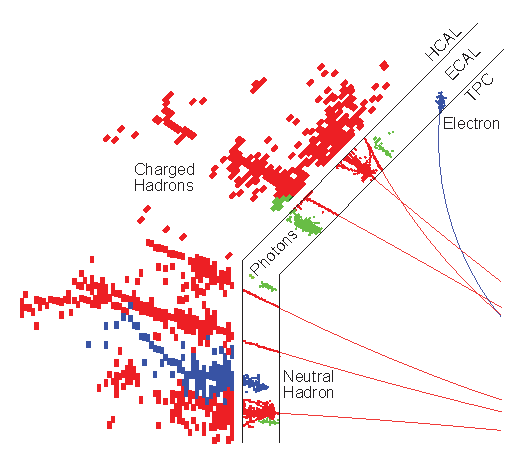
\includegraphics[width=0.45\textwidth]{{ILD/jetCLIC_ILD}}
\caption[A typical topology of a 250\,GeV jet.]
{A typical topology of a 250\,GeV jet, simulated with \CLICILD detector concept, taken from \cite{Marshall:2012ry}.}
\label{fig:detectorJetCLICILD}
\end{figure}


\FIGURE{fig:detectorJetCLICILD} is a typical topology of a 250\,GeV jet, simulated with \CLICILD detector concept. The particles with the calorimeter hits and tracks are labelled with different colours. Clusters of calorimeter hits in the highly granular \ECAL and \HCAL are associated with tracks from the inner tracking detector, \TPC. Photons are identified using the characteristics longitudinal and transverse electromagnetic shower profiles. Hadronic showers are separated from electromagnetic showers due to the small transverse spread of the electromagnetic shower.  Therefore, the inner tracking detector should be highly efficient and has very little material. For the calorimeter, the \ECAL and \HCAL, both should be highly granular. The material of the calorimeter should be dense and has a large ratio of interaction length to radiation length.

\subsection{Other requirements on the detector design}

Other physics requirement for the detectors for the \ILC and the \CLIC are summarised from \cite{Baer:2013cma,Linssen:2012hp}.

The requirement of tracking momentum resolution is driven by the Higgs boson mass resolution via Higgsstrahlung process, \eeTo{\PZ \PHiggs}. Higgs mass can be reconstructed precisely as the recoil mass against the \PZ momenta, which is obtained via \HepProcess{\PZ \to \APmuon \Pmuon}. For the \ILC operating at \rootSGeV{250}, the momentum resolution needs to be  $\sigma_{\pT} / \pT^2 \lesssim 5 \cdot 10^{-5} GeV^{-1}$. For the \CLIC at high \sqrtS, the momentum resolution needs to be  $\sigma_{\pT} / \pT^2 \lesssim 2 \cdot 10^{-5} GeV^{-1}$.

The performance requirement of the vertex detector is determined by efficient b-quark and c-quark tagging. The ability to identify secondary vertices and tracks, which are not originated from the interaction point, is the prerequisite for the flavour tagging. The impact parameter resolution can be written as
\begin{equation}
\sigma_{d_0}^2 = a^2 + \frac{b^2}{p^2\sin^2\left(\theta\right)}
\end{equation}
where $a$ is related to the point resolution and $b$ is related to multiple scattering. The requirements for both the \ILC and the \CLIC detectors are $a \lesssim 5 \mu{m}$ and $b \lesssim 15 \mu{m}GeV$

The lepton identification are should be over 95\% for effective lepton tagging. The forward converge of the detector should be down to a very low angle. This is more critical for the \CLIC as particles are boosted at high \sqrtS.

\section{International Large Detector}

Two detectors concepts have been designed for the \ILC to deliver the physics program. Precision tests for Standard Model requires an excellent jet energy resolution and di-jet mass reconstruction. Particle Flow Algorithms based event reconstruction meets the requirement and motivates the detector designs. For the best performance of the PFA, high granular calorimeter systems and highly efficient tracking systems are designed. The requirement to separate \PW and \PZ bosons in di-jet final states requires a jet energy resolution below 3.5\%. The momentum resolution of $5\times10^{-5}$\,GeV is motivated by the Higgs boson recoil reconstruction in the Higgs-strahlung.

Motivation for two detectors is to have multiple independent measurements within one collider for cross-checking, complementary measurements and competition between collaborations. Two detectors are both general purpose detectors. Silicon Detector, \SiD, is a compact detector with a large magnetic filed of 5\,T. It uses silicon tracking modules. The International Large Detector, \ILD, is a larger detector with a time projection chamber as the main tracking unit. Both detectors have high granular calorimeters optimised for the particle flow. A view of both detector concepts can be seen in \Figure{fig:detectorILDSiD}


The International Large Detector, \ILD, is a detector concept at the International Linear Collider, \ILC. The \ILD detector concept has been optimised in the view of the particle flow techniques. Particle flow approach to event reconstruction has shown to deliver the best possible jet reconstruction with proof-of-principle implementation such as \pandora {\Chapter{chap:Reconstruction}}. Each individual particles are reconstructed with the particle flow approach. For charged particles, calorimeter hits are associated with the tracks. The measurement of charged particle relies on the excellent tracking system resolution. Neutral particle reconstruction require fine spatial resolution of the calorimeters. These form the requirements for the detector designs and optimisations.

The particle flow paradigm requires topological information for individual particle reconstruction. The sub-detector systems need to have the spatial resolution to separate charged particles from neutral particles. The result is a highly granular calorimeters with a central tracking system with excellent momentum resolution. Longitudinal cross section of top quadrant of the \ILD detector concept, taken from \cite{Brau:2007zza}, is shown in \Figure{fig:ILD} From interaction point (\IP) outwards, there is a tracking system compromising a large time projection chamber (\TPC) augmented with silicon tungsten layer, highly granular electromagnetic calorimeters (\ECAL) and hadronic calorimeters (\HCAL), muon chambers, forward calorimeters (\FCAL), magnetic coils and iron yokes. Numbers are in units of mm.

This section will describe the sub-systems of the \ILD detector concept in the \ILD technical design report\cite{}, the ILD\_o1\_v05 option in \Mokka simulation. This detector concept has been used in studies described in subsequent chapters. The \ILD detector concept has been optimised and documented in previous documents, such as the letter of intent\cite{}. The \CLICILD detector concept for the \CLIC in the conceptual design report\cite{Linssen:2012hp} is a modified version of the \ILD, adapted to the \CLIC colliding environment. The differences between \ILD and \CLICILD can be seen in \Figure{fig:detectorILD} and \Table{tab:ILDvsCLICILD}, and are addressed in the discussion below.



\begin{figure}[tdbph]
\centering
  \begin{subfigure}[b]{0.45\textwidth}
    \includegraphics[width=\textwidth]{ILD/ILDview}
    \caption{}
    \label{fig:ILDview}
  \end{subfigure}
  \begin{subfigure}[b]{0.45\textwidth}
    \includegraphics[width=\textwidth]{ILD/SiD}
    \caption{}
    \label{fig:SiDview}
  \end{subfigure}
\caption[International Large Detector and the Silicon Detector for the International Linear Collider.]
{\FIGURE{fig:ILDview} and \Figure{fig:SiDview} show the view of the International Large Detector and the Silicon Detector for the International Linear Collider, taken from \cite{Baer:2013cma}.}
\label{fig:detectorILDSiD}
\end{figure}

\begin{comment}
The ILC has been designed to enable two experiments (SiD and ILD) sharing one interaction region using
a push-pull approach. This two-detector design is motivated by the enhanced scientific productivity of
past collider facilities which benefited from independent operation of multiple experiments, providing
complementary strengths, cross-checking and confirmation of results, reliability, insurance against
mishaps, competition between collaborations, as well as increased number of involved scientific
personnel. Figure 4.1 shows the arrangement of the two detectors in the detector hall.
Both detector designs are conceived as multi-purpose detectors, optimised for the broad range
of physics opportunities at the ILC. SiD is a compact, cost-constrained detector made possible
with a 5 Tesla magnetic field and silicon tracking. Silicon enables time-stamping on single bunch
crossings to provide robust performance, derived from immunity to spurious background bursts. The
highly granular calorimeter is optimised for particle-flow analysis. The ILD group has designed a
large detector with robust and stable performance over a wide range of energies. The concept uses
a tracking system based on a continuous-readout time-projection chamber combined with silicon

In order to realise the physics program, the ILC detectors face challenges requiring significant advances
in collider detector performance. The machine environment is benign by LHC standards, enabling
designs and technologies that are unthinkable at the LHC. However, the ILC environment poses its
own set of background issues that must be overcome. The ��Detailed Baseline Design�� of the SiD and
ILD detectors have been developed to achieve the requirements for all considered physics programs,
over the full range of centre-of-mass energies from 200 GeV up to 1TeV, as well as the possibility of
special running at the Z-pole.
The ILC physics opportunities place a premium on high-resolution jet energy reconstruction and
di-jet mass performance. Event reconstruction techniques based on the Particle Flow Algorithm (PFA)
have been developed to meet this challenge. This motivates highly granular electromagnetic and hadron
calorimeters and highly efficient tracking systems. New detector technologies and new reconstruction
algorithms based on the PFA approach achieve the needed precision in the reconstruction of jets of 3
to 4 percent for 100 GeV jets, set by the requirement to separate W and Z di-jet final states. The
requirements on momentum resolution for charged tracks (p/p2 of 5 �� 10.5 (GeV/c).1) are driven
by reconstruction of a Higgs boson recoiling from the associated Z boson decaying to a lepton pair in
the Higgs-strahlung process. Flavour and quark-charge tagging will be available at an unprecedented
level of performance as a result of the development of a new generation of vertex detectors. Particle
identification is achieved by the highly granular calorimeters and muon identification is aided by the
instrumented iron return yoke.
A very important element of the detector design work has been the common effort to develop and
apply simulation tools to realise realistic detector-performance estimates. A small group of experts
from both SiD and ILD have cooperated closely on this critical work.
To preserve this unprecedented performance, the inner detectors must accommodate very lowmass
detectors and supports. This is a significant challenge. The detector designs have achieved the
required light-weight support structures with minimal dead spaces. This was greatly simplified by the
ILC time structure of 1 millisecond bunch trains at 5 Hertz. This very sparse filling allows power for
many of the detector subsystems to be switched off between bunch trains (so-called power pulsing),
reducing the heat load and the need for cooling. The design of these power-pulsed systems presents a
significant challenge, including the need for quiescent currents.
27
\end{comment}


\section{Overview of \ILD sub-detectors}

The \ILD detector concept is designed as a general purpose detector. Closest to the interaction points are the precision a vertex detector and a tracking system. The tracking system consists of silicon tracking with a time projection chamber. Surrounding the tracking system is a high granular calorimeter system. The outer solenoid provides a magnetic field of 3.5\,T. The most outer iron return yoke acts as a muon calorimeter.


\subsection{Vertex Detector}

The pixel-vertex detector(\VTX) needs to be close to the interaction point to reconstruct secondary vertex. As the \TPC is the main tracking  detector, the \VTX mainly measures the impact parameter of tracks. The structure is three double layers with a barrel geometry. Double layer lowers the material budget and improves the impact parameter measurements. The first double layer is half length of the other two to avoid the high occupancy region of direct low omentulum hits from the incoherent pair background.



\subsection{Tracking Detectors}

The hybrid  tracking system is consists of a large volume time projection chamber (\TPC), a Silicon Inner Tracker (\SIT), a Silicon External Tracker (\SET) in the barrel region, a end cap tracking component (\ETD) behind the endplate of the \TPC, and a silicon forward tracker (\FTD) in the forward region. The \SIT, \SET, and \ETD are made up two single-sided strip layers tilted by a small angle. The \FTD is a system of two silicon-pixel disks and five silicon-strip disks.  The silicon envelope tracking system and the \TPC are shown in \Figure{fig:detectorTracking}.


The main part of the tracking system, the \TPC, can measure a large number of three dimensional spatial points. Continuous tracking allows precise reconstruction of non-pointing tracks. The \TPC is optimised for point resolution and minimum material, as required for the best calorimeter and particle flow performance.

The barrel silicon trackers improve the overall momentum resolution. They provide additional high precision space points and additional redundancy between the \TPC, the \VTX, and the calorimeters. The \FTD provide the low angle coverage which is not covered by the \TPC.


\begin{comment}
A system of silicon strip and pixel detectors surrounds the VTX detector. In the barrel, two
layers of silicon strip detectors (SIT) are arranged to bridge the gap between the VTX and the TPC.
In the forward region, a system of two silicon-pixel disks and five silicon-strip disks (FTD) provides
low angle tracking coverage.

The barrel silicon parts SIT and SET provide precise space points before and after the TPC; this
improves the overall momentum resolution, helps in linking the VTX detector with the TPC, and
in extrapolating from the TPC to the calorimeter. The coverage of the TPC with silicon tracking
is completed by the ETD, located within the gap separating the TPC and the end-cap calorimeter.
Together these systems help in calibrating the overall tracking system, in particular the TPC. The
good timing resolution of the silicon detectors relative to the time between bunches in the ILC together
with the high spatial precision helps in time-stamping tracks and assigning them to a given bunch
within an ILC bunch train.
\end{comment}


\begin{figure}[tdbph]
\centering
\includegraphics[width=0.45\textwidth]{ILD/Tracking}
\caption[A top quadrant view of the \ILD silicon envelope system]
{A top quadrant view of the \ILD silicon envelope system, \SIT, \SET, \FTD, and \ETD as included in MOKKA full simulation, adapted from the figure in \cite{Baer:2013cma}.}
\label{fig:detectorTracking}
\end{figure}


\subsection{Electromagnetic Calorimeter}

The Silicon-Tungsten sampling electromagnetic calorimeters in the \ILD consist of a nearly cylindrical barrel and two end cap systems, optimised for particle flow. The \ECAL measures photon energies and separates photons from other particles. The fine granular \ECAL also sits inside the \HCAL, which hosts the first part of the hadronic showers and greatly helps to separate hadronic showers.

The particle flow paradigm has a large impact on the \ECAL design with many requirements. In addition for the \ECAL to measure and separate photons, it also needs to reconstruct detail shower profiles to separate electromagnetic showers from hadronic showers, as approximately 50\% of hadronic showers starts in the \ECAL. These requirements can be fulfilled with an excellent three dimensional granular \ECAL.

From test beam data and simulation studies, a sampling calorimeter with longitudinal and transverse segmentation below one Moli\`{e}re radius and below one radiation length at the front the calorimeter is needed. The most compact design is realised with Tungsten as absorber material and silicon pad diodes as active material. A cross section of the \ECAL is shown in \Figure{fig:detectorILDECAL}. Tungsten is a dense material with a large ratio of interaction length to radiation length. This helps to separate electromagnetic showers from hadronic showers by making electromagnetic showers transversely narrow. Silicon pad size of 5.1 by 5.1 \,mm cover large areas. They are simple and reliable to operate. The choice of thin silicon layers offers a great spatial resolution at a cost of the energy resolution in favour of the particle flow.

The longitudinal segregation is a compromise between the cost and the performance. The total 30 layers, which is about 20\,cm, provides about 24 radiation lengths. The first 20 layers use 2.1\,mm thick absorber plates, which is twice finer sampling than the last 10 layers with 4.2\mm thick absorber plates. The test beam data with electron shows the energy resolution of the \ECAL concept to be $16.6/\sqrt{E(\ GeV)}\oplus1.1\%$, which is compatible with the values assumed for the full \ILD detector simulation.



\begin{figure}[tdbph]
\centering
\includegraphics[width=0.45\textwidth]{ILD/ILD_ECAL}
\caption[A cross section through electromagnetic calorimeter layers.]
{A cross section through electromagnetic calorimeter layers, taken from \cite{Baer:2013cma}.}
\label{fig:detectorILDECAL}
\end{figure}

\begin{comment}
The particle flow paradigm has a large impact on the design of the electromagnetic calorimeter system.
A key requirement is the capability of the system to separate overlapping showers from each other.
A calorimeter for particle flow thus needs to be able to do pattern recognition in the shower. The
electromagnetic section has a number of tasks to fulfill. It should be able to reconstruct photons
in the presence of close-by particles. It should be able to reconstruct the detailed properties of the
shower, such as shower shape, starting point and energy to distinguish early starting electromagnetic
showers from hadronic ones. It should be noted that about half of the hadronic showers start inside
the electromagnetic calorimeter. Thus an excellent three-dimensional granularity of the device is of
utmost importance.

The transverse and longitudinal segmentation of both calorimeters has been optimised based on
detailed simulation and test beam data. It has been shown that the granularity must be of the order
of X0 in all three dimensions. This implies that a sampling calorimeter is the best option for both
ECAL and HCAL. For the ECAL the most compact design can be realised with tungsten as absorber
material. For the HCAL iron is chosen as this allows an excellent energy resolution for hadrons at
manageable granularity.
For the ECAL, silicon pad diodes lead to the highest possible compactness (and effective Moli`ere
radius) and exhibit excellent stability of calibration. As an option scintillating strips with silicon
photo-sensor readout are studied, which provide a similar effective segmentation. The two technologies
can be combined in order to reach a cost-performance optimum.

In order to have a better separation of close-by showers in the calorimeter, a system with a
small Moli`ere radius is advantageous. Further help in the separation between electromagnetic and
hadronic showers can come from a large ratio between interaction length and radiation length. A
small radiation length will move the start of the electromagnetic shower earlier in the calorimeter,
while a large interaction length will reduce the fraction of hadronic showers starting in the ECAL.

The particle flow approach requires that the calorimeters are placed inside the magnetic coil,
see Sec. 1.2. This has a major impact on the layout of the detector, and on the cost. Therefore, a
compact calorimeter is preferred in order to minimise the overall physical thickness, which in turn
reduces the size of the coil. For the ECAL tungsten is a good choice for the radiator as it is dense, and
has a large ratio of interaction length to radiation length. The final system layout is a compromise
between performance and cost. The energy resolution scales with OT, where T is the individual
absorber plate thickness, while the cost scales linearly with the surface area of the readout layers. For
ILD a solution with 30 readout layers and a thickness of the ECAL of 24X0 has been chosen as the
baseline. The optimisation of the layout is ongoing.

For a chosen pad size of 5 . 5mm2 silicon pin diodes are a good choice. They can cover large
areas, are reliable and simple to operate, allow for a thin readout layer and can operate in the 3.5 T
strong central magnetic field. While the very thin silicon layers offer excellent performance for the
tracking capabilities of the calorimeter, the energy resolution is somewhat degraded. Here a less
compact device, with a thicker readout layer, will show better performance.

The requirements on granularity, compactness and particle separation lead to the choice of a
sampling calorimeter with tungsten (radiation length X0 = 3.5 mm, Moliere Radius RM = 9 mm and
interaction length = 99 mm) as absorber material. This allows for a compact design with a depth
of roughly 24 X0 within 20 cm and, compared to e.g. lead, a better separation of electromagnetic
showers generated by near-by particles. To achieve an adequate energy resolution, the ECAL is
longitudinally segmented into 30 layers, possibly with varying tungsten thicknesses. In order to
optimise the pattern recognition performance, the active layers (either silicon diodes or scintillator)
are segmented into cells with a lateral size of 5 mm.
\end{comment}

\subsection{Hadronic Calorimeter}

The requirements of sampling hadronic calorimeter is, again, driven by the need of the particle flow. The need of three dimensional granularity in transverse and logistically direction is satisfied by a sampling calorimeter.



The principle role of the \HCAL is to separate neutral hadron showers from other particles, and to measure neutral hadron energies. The neutral hadron contribution of  the jet energy is around 10\% on average. A moderate fine  granular \HCAL is a good balance between cost and performance. The chosen layout is 48 longitudinal layers with 3 by 3\cm scintillator tiles, using an analogue read out system. The layout of a technological prototype, the "EUDET prototype" is shown in \Figure{fig:detectorAHCAL} \cite{Collaboration:2011jka}.

The longitudinal system provide about 6 radiation lengths including the \ECAL, which is sufficient to contain the hadronic showers. The transverse cell sizes has been optimised for the best jet energy resolution. It is found that no substantial gain below 3\,cm and performance degradation above 3\,cm. Hence 3\,cm cell size is chosen for the \HCAL. The jet energy resolution as a function of \HCAL scintillator cell size with different jet energies is shown in \Figure{fig:detectorHCALoptimise}.

For the absorber material, stainless steel is chosen for mechanical and calorimetric reasons. Steel allows a self-supporting structure without auxiliary supports. Also steel has a moderate ratio of interaction length to radiation length.




\begin{figure}[tdbph]
\centering
  \begin{subfigure}[b]{0.45\textwidth}
    \includegraphics[width=\textwidth]{ILD/ILD_AHCAL}
    \caption{}
    \label{fig:detectorAHCAL}
  \end{subfigure}
  \begin{subfigure}[b]{0.45\textwidth}
    \includegraphics[width=\textwidth]{ILD/HCALoptimise}
    \caption{}
    \label{fig:detectorHCALoptimise}
  \end{subfigure}
\caption[CALICE AHCAL technological prototype module and  jet energy resolution.]
{\FIGURE{fig:detectorAHCAL} shows the schematic view of a CALICE AHCAL technological prototype module. \FIGURE{fig:detectorHCALoptimise} shows the jet energy resolution as a function of the hadronic calorimeter scintillator cell sizes, with different energies. Both figures are taken from \cite{Baer:2013cma}.}
\label{fig:detectorHCAL}
\end{figure}


\begin{comment}
The role of the HCAL is to separate the deposits of charged and neutral hadrons and to precisely
measure the energy of the neutrals. Their contribution to the jet energy, around 10% on average,
fluctuates over a wide range from event to event, and the accuracy of the measurement is the
dominant contribution to the particle flow resolution for jet energies up to about 100 GeV. For higher
energies, the performance is dominated by confusion, and both topological pattern recognition and
energy information are important for correct track cluster assignment.


This is followed by a highly segmented hadronic calorimeter (HCAL) with up to 48 longitudinal
samples and small transverse cell size. Two options are considered, both based on a Steel-absorber
structure. One option uses scintillator tiles of 3 . 3 cm2, which are read out with an analogue
system. The second uses a gas-based readout which allows a 1.1 cm2 cell geometry with a binary or semi-digital readout of each cell.


The HCAL is optimized to measure neutral hadrons
well and thus has to provide the topological resolution power for separating them from the showers of
the much more abundant charged hadrons which must be matched with tracks.


The transverse and longitudinal segmentation of both calorimeters has been optimised based on
detailed simulation and test beam data. It has been shown that the granularity must be of the order
of X0 in all three dimensions. This implies that a sampling calorimeter is the best option for both
ECAL and HCAL. For the ECAL the most compact design can be realised with tungsten as absorber
material. For the HCAL iron is chosen as this allows an excellent energy resolution for hadrons at
manageable granularity.



The role of the HCAL is to separate the deposits of charged and neutral hadrons and to precisely
measure the energy of the neutrals. Their contribution to the jet energy, around 10% on average,
fluctuates over a wide range from event to event, and the accuracy of the measurement is the
dominant contribution to the particle flow resolution for jet energies up to about 100 GeV. For higher
energies, the performance is dominated by confusion, and both topological pattern recognition and
energy information are important for correct track cluster assignment.




The HCAL is conceived as a sampling calorimeter with steel absorber and scintillator tiles
(analogue HCAL) or gaseous devices (semi-digital HCAL) as active medium. Due to the rigidity of
stainless steel, a self-supporting structure without auxiliary supports (dead regions) can be realised.
Moreover, in contrast to heavier materials, iron with its moderate ratio of hadronic interaction length
(.I = 17 cm) to electromagnetic radiation length (X0 = 1.8 cm) allows a fine longitudinal sampling
in terms of X0 with a reasonable number of layers in a given total hadronic absorption length, thus
keeping the detector volume and readout channel count at an acceptable level. This fine sampling is
beneficial both for the measurement of the sizeable electromagnetic energy part in hadronic showers
and for the topological resolution of shower substructure, needed for particle separation and weighting.
Two baseline technology options have been developed, the scintillator-tile based AHCAL and the
Glass Resistive Plate Chamber (GRPC) based SDHCAL.
\end{comment}

\subsection{Solenoid}

A large superconducting solenoid outside the calorimeters produces a nominal  3.5\,T magnetic field. 


\subsection{Yoke and Muon system}

An iron yoke instrumented with scintillator strips active layers returns the magnetic flux, and acts as a muon detector and tail catcher calorimeter at the same time. The layout is shown in \Figure{fig:detectorILDMuon}. The agreed maximum magnetic field at 15\,m radial distance from the detector is 50 Gauss to ensure safety \cite{Parker:21354}. A highly efficient muon detector is provided by the 3 by 3\,cm scintillator strips. As a tail catcher calorimetry, the first layer of the muon detector, catches the energy leakage from the \HCAL and the \ECAL. It has been shown a 10\% improvement of single particle energy resolution is possible with the tail catcher \cite{CALICE:2012aa}.



\begin{figure}[tdbph]
\centering
\includegraphics[width=0.45\textwidth]{ILD/ILD_Muon}
\caption
{Sensitive Layers of the \ILD muon system, taken from \cite{Baer:2013cma}.}
\label{fig:detectorILDMuon}
\end{figure}

\begin{comment}
the iron Yoke has been instrumented with scintillator based active layers. At the
moment tiles with 3 . 3 cm2 granularity are used, for muon detection and serving as a tail
catcher for the HCAL; this is different than the detector baseline which uses 3 cm wide and 1
m long strips;

During beam operation the IR hall has to be accessible due to the push-pull concept. Since all
activities in a high magnetic field are very cumbersome and potentially dangerous, a field limit of 50 G
at 15 m radial distance from the beam line was agreed upon [354]. Two- and three-dimensional FEM
field calculations were done using the CST EM Studio program, varying the thickness and geometry
of the iron in the barrel and end-caps until the goal of less than 50 G at 15 m radial distance was
achieved.



An iron yoke, instrumented with scintillator strips or resistive plate chambers (RPCs), returns
the magnetic flux of the solenoid, and, at the same time, serves as a muon filter, muon detector and
tail catcher calorimeter

A stable, highly efficient muon identification system with excellent hadron rejection is an important
requirement to meet the physics goals of the ILD detector. The ILD muon system provides a number
of measurement stations outside the solenoid coil, which supplement the measurements taken with
the calorimeter system and the tracker. It is used to identify the muons and to act as a tail catcher, to
recover energy which is leaking out of the back of the calorimeter. However, the barrel part location
behind the coil limits its role to fairly high momentum particles.
The muon system/ tail catcher instruments the iron return yoke in the barrel and in the forward
region. The yoke barrel part is equipped with one sensitive layer in front of the iron yoke, 10 layers
spaced 14 cm apart, followed by three sensitive layers spaced by 60 cm apart. The forward part of the
yoke is equipped with 10 layers spaced by 14 cm, followed by two sensitive layers spaced by 60 cm.
The overall layout of the muon system/ tail catcher is shown in Figure

The first layers of the muon system serve as a tail catcher, measuring the energy which leaks through
the end of the calorimeter system. Figure III-4.5 shows the effect of an ideal tail catcher (no dead
material between the calorimeter and the tail catcher) and the realistic scenario at ILD, with two
interaction lengths of material in front of the tail catcher, as a function of the total depth of the
calorimeter system. For 6 ., the value for the ILD calorimeter system, a roughly 10% improvement is
possible with the tail catcher [348].
A prototype of the muon system/tail catcher was successfully tested during the 2007-2012
CALICE test beam campaign with ECAL and analogue HCAL. A tail catcher was placed behind the
HCAL instrumented with scintillator strips and readout with SiPMs [348]. Results from the tests
show that the proposed system delivers the anticipated performance and thus validates the technology
needed to built a muon system for ILD.
\end{comment}

\subsection{Very Forward Calorimeters}

The forward region detectors provide luminosity measurements and forward coverage of calorimeters. A system of precision and radiation resistent calorimeters are required. The luminosity calorimeter counts  Bhabha scattering to measure the luminosity to precision of $10^{-3}$ at 500\,GeV centre-of-mass energy. The beam calorimeter (\BeamCAL) extend the forward coverage, which are hit by many beamstrahlung pairs after each bunch corssing. \BeamCAL estimates a bunch-by-bunch luminosity. An additional hadron calorimeter, \LHCAL, at the forward region extends the angular coverage of the \HCAL to that of the \LumiCAL. Electron tagging is possible with the very forward calorimeters\cite{sailer2012radiation}, which aids event reconstruction at high centre-of-mass energy.


\begin{figure}[tdbph]
\centering
\includegraphics[width=0.45\textwidth]{ILD/ILD_forward}
\caption[The forward calorimeters of the \ILD.]
{The forward calorimeters of the \ILD, taken from \cite{Baer:2013cma}. \LumiCAL, \BeamCAL, and \LHCAL are the luminosity calorimeter, beam calorimeter, and forward hadronic calorimeter.}
\label{fig:detectorILDForward}
\end{figure}

\begin{comment}

At very forward angles, below the coverage provided by the ECAL and the HCAL, a system of
high precision and radiation hard calorimetric detectors (LumiCAL, BeamCAL, LHCAL) is foreseen.
These extend the calorimetric coverage to almost 4fi, measure the luminosity, and monitor the quality
of the colliding beams

Two special calorimeters are foreseen in the very forward regions of the detector [324], denoted
hereafter as LumiCal and BeamCal. LumiCal will measure the luminosity with a precision of better
than 10��3 at 500 GeV centre-of-mass energy1, and BeamCal will perform a bunch-by-bunch estimate
of the luminosity and, supplemented by a pair monitor, assist beam tuning when included in a fast
feedback system [325]. Both calorimeters extend the detector coverage to low polar angles, important
e.g. for new particle searches with missing energy signature [326]. The additional low angle hadron
calorimeter LHCAL extends the coverage of the hadron calorimeter to the polar angle range of
LumiCal. A sketch of the design is shown in Figure III-3.24.
LumiCal is positioned in a circular hole of the end-cap electromagnetic calorimeter ECAL.
BeamCal is placed just in front of the final focus quadrupole. LumiCal covers polar angles between
31 and 77 mrad and BeamCal between 5 and 40 mrad.
Due to the high occupancy originating from beamstrahlung and two-photon processes, both
calorimeters need a fast readout. In addition, the lower polar angle range of BeamCal is exposed to a
large flux of low energy electrons, resulting in radiation depositions up to one MGy per year. Hence,
radiation hard sensors are needed.

\end{comment}


%This section will describe sub-systems from small to large radius.



\begin{comment}
The International Large Detector (ILD) is a concept for a detector at the International Linear Collider,
ILC [198]. In a slightly modified version, it has also been proposed for the CLIC linear collider [199].
The ILD detector concept has been optimised with a clear view on precision. In recent years
the concept of particle flow has been shown to deliver the best possible overall event reconstruction.
Particle flow implies that all particles in an event, charged and neutral, are individually reconstructed.
This requirement has a large impact on the design of the detector, and has played a central role in
the optimisation of the system. Superb tracking capabilities and outstanding detection of secondary
vertices are other important aspects. Care has been taken to design a hermetic detector, both in
terms of solid-angle coverage, but also in terms of avoiding cracks and non-uniformities in response.
The overall detector system has undergone a vigorous optimisation procedure based on extensive
simulation studies both of the performance of the subsystems, and on studies of the physics reach
of the detector. Simulations are accompanied by an extensive testing program of components and
prototypes in laboratory and test-beam experiments.
Figure III-1.1
View of the ILD detector
concept.
The ILD detector concept has been described in a number of documents in the past. Most
recently the letter of intent [198] gave a fairly in depth description of the ILD concept. The ILD
concept is based on the earlier GLD and LDC detector concepts [200, 201, 202]. Since the publication
of the letter of intent, major progress has been made in the maturity of the technologies proposed for
ILD, and their integration into a coherent detector concept
\end{comment}




\section{\CLIC versus \ILC}


The two main differences between \CLIC and \ILC are the high centre-of-mass energy and the high bunch charge density leading to significant beam related backgrounds.  Within a bunch train, there is 0.5\,ns between bunch crossings at CLIC.  There are two main sources of beam induced backgroun: incoherent electron pairs from  photon (real or virtual) interactions with individual particles of the other beam, and interactions of two photons from the colliding beams. These differences leads to a modification in the detector design and the reconstruction software for the \CLIC. A comparison of \CLICILD and \ILD longitudinal cross sections can be seen in \Figure{fig:detectorILD}. A comparison of key parameters of the \ILD and \CLICILD detector concepts is shown in \Table{tab:ILDvsCLICILD}.

\begin{table}[htbp]
\centering
\smallskip
\begin{tabular}{l  r  r }
\hline
Concept &  \ILD & \CLICILD \\
\hline
Tracker & TPC/Silicon & TPC/Silicon \\
Solenoid Field (T) & 3.5 & 4 \\
Solenoid Field Bore (m) & 3.3 & 3.4 \\
Solenoid Length (m) & 8.0 & 8.3 \\
\VTX Inner Radius (mm) & 16 & 31 \\
\ECAL $r_{min}$ (m) & 1.8 & 1.8 \\
\ECAL $\Delta{r}$ (mm) & 172 & 172 \\
\HCAL Absorber B / E & Fe & Fe / W \\
\HCAL Interaction Length & 5.5 & 7.5 \\
Overall Height (m) & 14.0 & 14.0 \\
Overall Length (m) & 13.2 & 12.8 \\
\hline

\hline
\end{tabular}

\caption[A comparison of key parameters of the \ILD and \CLICILD detector concepts.]
{ A comparison of key parameters of the \ILD and \CLICILD detector concepts. \ECAL $r_{min}$ is the smallest distance from the calorimeter to the main detector axis. \HCAL Absorber B / E indicates the absorber material for the barrel (B) and the endcap (E). The table is adapted from \cite{Linssen:2012hp}.}
\label{tab:ILDvsCLICILD}
\end{table}

\begin{figure}[tdbph]
\centering
  \begin{subfigure}[b]{0.45\textwidth}
    \includegraphics[width=\textwidth]{ILD/ILD}
    \caption{}
    \label{fig:ILD}
  \end{subfigure}
  \begin{subfigure}[b]{0.35\textwidth}
    \includegraphics[width=\textwidth]{ILD/CLIC_ILD}
    \caption{}
    \label{fig:CLIC_ILD}
  \end{subfigure}
\caption[Longitudinal cross section of top quadrant of the \ILD and the \CLICILD detector concepts.]
{\FIGURE{fig:ILD} and \FIGURE{fig:ILD} shows longitudinal cross section of top quadrant of the \ILD and the \CLICILD detector concepts, taken from \cite{Baer:2013cma} and \cite{Linssen:2012hp} respectively. From interaction point (\IP) outwards, there is a tracking system compromising a large time projection chamber (\TPC) augmented with silicon tungsten layer, highly granular electromagnetic calorimeters (\ECAL) and hadronic calorimeters (\HCAL), muon chambers, forward calorimeters (\FCAL), magnetic coils and iron yokes. Numbers are in units of mm.}
\label{fig:detectorILD}
\end{figure}



\subsection{\CLICILD versus \ILD}



There are two detector concepts studied in the \CLIC conceptual design report \cite{Linssen:2012hp}, \CLICILD and \CLICSiD. The \CLICILD detector concept is based on the \ILD design. They share similarities due to similar physics motivations. Only differences are highlighted here.

For the vertex detector, the first layer is moved outwards by 15\,mm due to a larger high occupancy region with higher centre-of-mass energy. The detector is also required to provided time stamping at nanoseconds level, which would be a different detector.

For the tracking detector, the same silicon-\TPC hybrid structure is used. The outer silicon tracking system is more important at the \CLIC to achieve a high momentum resolution at high centre-of-mass energy, as it is challenging using a \TPC to sperate two tracks in high energy jets and to identify events in the collection of 312 bunch crossings in 156\,ns. The solid angle coverage of the tracking detector is $12\degree \lesssim \theta \lesssim 168\degree$

The same \ECAL from the \ILD is assumed, as the requirements of a \CLIC detector are satisfied. The increased centre-of-mass energy results in extra energy leakage. But only a small fraction of particles are affected and the leakage is controlled by the \HCAL.

For the \HCAL, extra layers are added to contain the hadronic shower at high energy. The increased thickeners is justified by the simulation studies, where the jet energy resolution degrades quickly for a thinner \HCAL. To sustain the same inner bore radius, a more dense material, Tungsten, is chosen as the absorber material in the \HCAL barrel. 

The magnetic filed is increased to 4\,T  for a better performance at a high centre-of-mass energy. Due to the different magnetic field strength, the iron yoke thickness increase to 230\,cm.

The \CLICILD adopted a similar very forward calorimetry system as that of the \ILD. Dimension of the elements are changed due to a difference in the crossing angle (20\,mrad for \CLIC and 14\,mrad for \ILC). A comparison of \LumiCAL and \BeamCAL at \ILD and \CLICILD is shown in \Table{tab:detectorForwardILDvsCLICILD}.

Modifications to the design due to \CLIC 3\,TeV centre-mass-of energy can be found in \cite{Linssen:2012hp}.

\begin{table}[htbp]
\centering
\smallskip
\begin{tabular}{l l r  r }
\hline
 & &  \ILD & \CLICILD \\
\hline
\LumiCAL & geometrical acceptance (mrad)& 31 - 77 & 38 - 110 \\
& fiducial acceptance (mrad) & 41 - 67 & 44 - 80 \\
& z (start) (mm) & 2450 & 2654 \\
& number of layers (W + Si) & 30 & 40 \\
\hline
\BeamCAL & geometrical acceptance (mrad)& 5 - 40 & 10 - 40 \\
& z (start) (mm) & 3600 & 3281 \\
& number of layers (W + sensor) & 30 & 40 \\
& graphite layer thickness (mm) & 100 & 100 \\
\hline
\hline
\end{tabular}
\caption[Comparison of \LumiCAL and \BeamCAL at \ILD and \CLICILD .]%
{Comparison of \LumiCAL and \BeamCAL at \ILD and \CLICILD . The table is adapted from \cite{Linssen:2012hp}. }
\label{tab:detectorForwardILDvsCLICILD}
\end{table}

%Beam Calorimeter acceptance is defined as \absCosTheta is between  0.01 and 0.04\,rad and length in z direction is between 3181 and 3441\,mm. Luminosity Calorimeter acceptance is defined as \absCosTheta is between  0.038 and 0.11\,rad and length in z direction is between 2539 and 2714\,mm.




  \chapter{Simulation and Reconstruction}
\label{chap:Reconstruction}

\chapterquote{How to open a pandora box?}%
{A wise Chinese}%: Blackwood's Magazine May 1830

%As previously stated, this document focus on the \ILD and \CLICILD detectors. Due to the similarity, we often only discuss one detector to avoid the repetition. The difference in detectors will be stated if applicable.

In previous chapters, overviews of the theory and the future linear collider experiments have been described. Since the work presented in this document is for future collider, simulation and monte carlo method is used throughout the document. In this chapter, the simulation and event reconstruction chain are discussed, with emphasis on the \pandora event reconstrcution, which provides the background for the photon reconstruction algorithms in \Chapter{chap:Reconstruction}.

Simulation and reconstruction of events for the future Linear Colliders, \ILC and \CLIC, share common software framework. The noticeable difference will be discussed.

\section{Monte Carlo event generation}

For the simulated study, Monte Carlo (MC) event generation is the first step. Most events, electron-positron interaction, are generated with WHIZARD software, \cite{whizard,Moretti:2001zz}, with no polarisation of the electron and positrons. Some simple events are generated with HEPEVT. PYTHIA \cite{Sjostrand:1995iq} is used to describe parton showering, hadronisation and fragmentation. The parameters for PYTHIA are tuned to OPAL data from the LEP \cite{Alexander:1995bk}. TAUOLA \cite{Jadach:1993hs} debrides the tau lepton decay with correct spin correlations of the day products. The Initial State Radiation (\ISR) is simulated in WHIZARD with the \ISR photons being collinear with the beam direction. The Final State Radiation (\FSR) is simulated with default parameters in PYTHIA.

For the \CLIC simulated samples, the luminosity spectrum, which is generated with GUINEAPIG \cite{Schulte:1999tx}, is simulated in WHIZARD. The \ggHad background events are hadronised with PYTHIA, and superimposed on the physics process simulations to save computational resources.

TODO
\ggHad simulation -5 to 25ns etc


\section{Event Simulation}

The event simulation software is GEANT4 \cite{Agostinelli:2002hh}, and the detector geometry description is provided by MOKKA \cite{MoradeFreitas:2002kj}.  QGSP\_BERT physics list is used to describe the hadronic showers decay in the detector.


%Simulation and reconstruction of events for the future Linear Colliders share common software framework. Simulated events are generated with Whizard software \cite{}. Pythia describes hadronisation and Tauola simulates correct spins of tau lepton decay products.  Whizard allows events simulation without initial state radiation, and can simulate electron beam interaction. For the \CLIC detector, electron beam induced background events are simulated and reconstructed. These events are superimposed on the physics process to save computational resources.


\section{Event Reconstruction}

Reconstruction software runs in Marlin framework \cite{Gaede:2006pj}, as a part of the \ilcsoft. Event reconstruction contains following steps: digitisation of simulated calorimeter hits, reconstruction of tracks in the tracking system using pattern recognition algorithms, and particle flow objects (\PFOs)reconstruction with \pandora\cite{Thomson:2009rp,Marshall:2012ry}. Reconstruction does not include calorimeters hits in the forward calorimeters, due to computational reasons  (see \Section{sec:doubleHiggsForwardElectron}).

For the \CLIC detector simulations, suppression of \ggHad background is performed.

Details of the reconstruction can be found in \cite{Brau:2007zza,Linssen:2012hp}. Particle flow reconstruction via \pandora will be discussed in details, which provides the background for the photon reconstructions in \pandora in \Chapter{chap:Reconstruction}.



\section{\pandora}
\label{sec:pandoraPandoraPFA}
Tradition calorimetric approach is unable to meet the mass and energy requirements for the future linear collider. The particle flow approach with \pandora has a proof-of-principle demonstration of its capability to reach required resolution. The particle flow approach also put stringent requirements on the detector design, which is described in \Chapter{chap:Detector}. By associating calorimeter hits to the tracks, around 60\% of the jet energy from charged particles is measured by the tracker, which has a much better resolution than the calorimeter. Small cell sizes of the calorimeters are required to identify hits from different particles. The traditional sum of calorimeter cell energies is replaced by particle flow reconstruction algorithms, a complex pattern recognition problem.  The \pandora algorithm has been developed and used in the \ILC and \CLIC simulation studies.

Started with the \ILD detector concept, \pandora has been adapted to the \CLIC condition and shows its ability to deliver required energy resolutions \cite{Linssen:2012hp}. Recent the code base of the \pandora has been restructured. The core base codes for basic object and memory managements are factorised in the Pandora C++ Software Development Kit\cite{Marshall:2015rfa}. There are over 60 linear collider specific reconstruction algorithms, each aims to address a particular topological in the reconstruction.

In the subsequent paragraphs, the main steps in the \pandora reconstructions are described. The details of the reconstruction can be found in cite{Thomson:2009rp,Marshall:2012ry,Marshall:2015rfa}.

Inputs of \pandora are digitised calorimeter hits and reconstructed tracks. The output are reconstructed particles with four-momenta, Particle Flow Objects (\PFOs).

\subsection{Track selection}
\label{sec:pandoraPandoraTrack}
Tracks from the tracking system are selected based on their topological properties, how likely they are from physical processes, and whether they are consistent with the tracker resolution. Tracks passed the selection are used for the subsequent reconstruction.  Special topologies of tracks are identified, such as when a neutral particle decays or converts into a pair of charged tracks, leaving a ``V0''  shape tracks. This is identified by searching for a pair of tracks originated from a single point. Another topologies include ``kinks'' , when a charged particle decays to a single charged particles with neutral particles, and ``prongs'', when a charged particles decays to multiple charged particles. This information are stored and passed on to the subsequent reconstruction, along side with the helical track fit (using last 50 reconstructed hits) and the track projection to the front of the \ECAL.

\subsection{Calorimeter selection}

The input information of a calorimeter hit is the position, the layer in the calorimeter and the energy response from the calorimeter.

Calorimeter hits are selected based on a series of criterion. The selected hits need to have energies above the threshold, using the conversion of a minimum ionising particle (MIP) equivalent, and using directly the converted energy. Similar to tracks, only calorimeter passed the selection are used in later steps.

Geometry information and likelihood of the hit originated from a minimum ionising particle (MIP) are calculated.

Isolated hits, often originated from low energy neutrons in a hadronic shower, are difficult to associate to the correct hadronic shower. They are identified and not used in the clustering. But their energy is added in the very last particle flow object (PFO) creation step.

\subsection{Cone Clusters Algorithm}
\label{sec:pandoraConeCluster}
Before discussing the rest of the \pandora reconstruction, it is necessary to introduce the cone based clustering algorithm, which is widely used in the calorimeter in \pandora. The clustering algorithm produces basic working objects, \clusters.


\begin{figure}[tbph]
\centering
{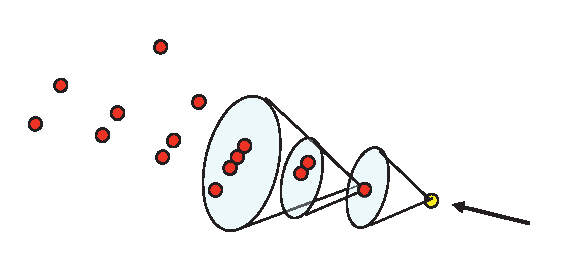
\includegraphics[width=0.5\textwidth]{pandora/coneClustering}}%
\caption{Illustration of the cone clustering algorithm, taken from \cite{Marshall:pandoraLC}}
\label{fig:pandoraConeClustering}
\end{figure}

There are two main types of clustering algorithms: cone based and sequential combination (see \Section{}). The main clustering scheme \pandora is cone clustering, for grouping calorimeter hits. Illustrated in \Figure{fig:pandoraConeClustering}, cone clustering has a specified opening angle of the seed hit. Because the direction of particle flows is largely unchanged from the originated particle, whether it is a electromagnetic shower, QCD radiation or hadronisation, these cone clusters have similar direction and energy to the originated particle. Therefore it is applicable to use cone based clustering algorithms for building clusters.

The seed for the cone clustering is typically the projection of a energetic track to the front of the \ECAL. A high  energy calorimeter hit can also be used as a seed. A cone with a specified opening angle and depth will be formed around the seed. The \fourMomentum of calorimeter hits sum to the cone's \fourMomentum.

TODO
Build from inner to outer, then every layer outer in inner see Mark's paper

\subsection{Particle Identification}
\label{sec:particleID}

Dedicated particle identification algorithms aim to identify muons and photons before associating calorimeter hits to tracks. The details of the photon reconstruction algorithms and photon related algorithms are described in \Chapter{chap:Reconstruction}. By removing the hits from muons and photons, the reconstruction of charged particles is improved as it reduce the pattern recognition problem. Identified muons and photons do not participate in the clustering and re-clustering stages, but re-entre the construction at the fragment removal stage (see \Section{sec:pandoraFragmentRemoval}).

\subsection{Clustering}

The cone clustering algorithm described in \Section{sec:pandoraConeCluster} is used to group calorimeter hits from innermost to outmost pseduo-layer. The output \clusters are further processed, merged or split based on their topological properties.

\subsection{Topological cluster association}

Initial clustering scheme is aggressive at splitting clusters. Small clusters are merged  based on clear topological signatures. These merging signatures include combining track segments, connecting tack segments with gaps, connecting track segment to a hadronic shower, and merging clusters when they are within close proximity.

\subsection{Track-cluster association}

Clusters are associated to tracks, according to the proximity of the first layer of the cluster and the track projection to the front of the \ECAL.


\subsection{Re-clustering}

The cluster association scheme work well for low energy (less than 50\,GeV) jet. For a high energy jet, particles and the subsequent hadronic showers are more boosted and more likely to overlap each other. Therefore, it is important to re-cluster based on the compatibility of the cluster energy and the associated track momentum. A cluster may be split into two. Two clusters maybe be re-clustered based on the track-cluster association. The re-clustering algorithm is applied iteratively to find a more correct clustering of calorimeter hits.

\begin{comment}
\subsection{Photon identification}

The neutral clusters are tested against an expected photon electromagnetic shower profile. The longitudinal shower profile for a photon cluster is required to be similar to a expected electromagnetic shower profile, with the discrepancy being smaller than a threshold.
\end{comment}

\subsection{Fragment removal}
\label{sec:pandoraFragmentRemoval}
The late stage of the reconstruction will focus on merging low energy clusters, especially non-photon neutral clusters. These neutral clusters are likely to be fragments of charged clusters, instead of being a physical particle. The merging criterion are mostly based on the proximity and the energy comparison.

One algorithm will attempt to split up photon clusters, where each is originated from two close by photons. Photon related algorithms are described in details in \Chapter{chap:Reconstruction}.



\subsection{Particle Flow Object Creation}
\label{sec:pandoraPFOcreation}

% double counting taking care in pandora
Particle Flow Objects (PFOs) are created at the last step. Tracks are associated to the clusters based on the proximity. Simple but effective particle identification for electrons, muons are applied. Photon identifications have been applied at various stages of the reconstruction.

PFOs are the output of the \pandora reconstruction. The four-momentum of these PFOs are  used heavily for the downstream analysis. The electron, muon and photon identification are  also used in physics analysis, such as one described in \Chapter{chap:Tau}.

\section{MC truth linker}
Hits contribution to MC particle.
Main contributed MC particle from energy weighted hits
Main contributed Jets etc. from hits
\section{\CLIC specific simulation and reconstruction}



\section{Luminosity spectrum}



\section{Suppression of \ggHad backgrounds}
\label{sec:pandoraggHad}


For the CLIC, significant \ggHad background is present. It is crucial to remove the beam induced background as they don't represent the underlying physics process.

Two Marlin process has been developed to suppress these background, a track selector and a PFO selector\cite{Marshall:2012ry}.

The track selector aims to remove poor quality and fake tracks. It places simple quality cut and a simple time of arrival cut. If the arrival time of the track at the front of the \ECAL, using the helical fit, differs more than 50\,ns from using a straight line fit, the track will be rejected.

The PFO selector utilise the high spatial resolution from the high granular calorimeter. PFOs from \ggHad often have low \pT and have a range of time. PFOs from physics processes have a range of \pT, and have time close to the brunch crossing time. These two distinctive features allow \ggHad background to be separated. The optimal suppression uses different \pT and time cuts for the central part of the detector, and for the forward part of the detector, and uses different cuts for photons, neutral PFOs and charged PFOs. Three configurations of these cuts are developed, namely ``loose'', ``normal'', and ``tight'' selections. As the name suggested, ``loose'' selection corresponds to a looser cut of \pT and time. The optimal configuration depends on the \sqrtS of the collision, and the physics process to study.

The background suppression is used in analysis described in \Chapter{chap:DoubleHiggs}
TODO add efficiency table pandora
TODO add timing pT cut and table of energies

\section{\CLIC simulated particle masses} 

\section{Reconstruction Processors}

Automated analysis is the only way to deal with the vast amount of data generated in the high energy physics. In the last chapter we described the automated reconstruction tools in details. This chapter is dedicated to the common automated analysis tools and techniques, which will be used in the analysis described in subsequent chapters.

For the linear collider, thanks to the high granular calorimeter, the starting point for analysis would be individual Particle Flow Objects, as well as individual tracks. Each of the PFOs encodes four-momentum and position information. For tracks, they would have momentum and position information.

However, sometimes it is interesting to group PFOs and tracks into jets, where a jet is the result of hadronisation process from high energy particles like quarks or gulons.

\section{Jet algorithm}

A jet is typically a visually obvious structure in a event display. The momentum and the direction of a jet tend to resemble the originated particle. Despite the relative easiness of identifying jets visually, it presents a challenge for a pattern recognition program to identify jets effectively and efficiently.

Early work on jet finding started in 1977 \cite{Sterman:1977wj}, where later development can be found in reviews \cite{Moretti:1998qx,Salam:2009jx,Ali:2010tw}.

There are two large families of jet finding algorithm, cone based algorithms, and sequential combination algorithms. Cone based algorithm is briefly discussed in \Section{sec:pandoraConeClustering} in the context of the \pandora user case.

Sequential combination algorithms typically calculate a pair-wise distance metric. Pairs with the smallest metric will be combined. The metric will be calculated and updated after a combination. This procedure will be repeated until some stopping criterion are satisfied.
%, and a pair with smallest metric will be combined.

The chosen jet algorithm implementation is FastJet C++ software package \cite{Cacciari:2011ma,Cacciari:2005hq}, providing a wide range of jet finding algorithms. The implementation in Marlin software package is called MarlinFastJet. The symbols in the subsequent discussion follow the convention in \cite{Cacciari:2011ma}
\paragraph{\kt algorithm}

longitudinally-invariant \kt algorithm \cite{Catani:1993hr,Ellis:1993tq} is one of the common sequential combination algorithms for \pp collider experiment. In the inclusive variant, the symmetrical pair-wise distance metric between particle $i$ and $j$, and the beam distance, are defined as
\begin{equation}
&d_{ij} = d_{ji} = \min\!\parenths{\pT_{i}^{2},\!\pT_{j}^{2}}\frac{\DeltaOf{R_{ij}^{2}}}{R^{2}}, \\
&d_{iB} = \pT_{i}^2,
\end{equation}
where $\pT_{i}$ is the transverse momentum of particle $i$ with respect to the beam ($z$) direction, and $\DeltaOf{R_{ij}^{2}}$ is the measurement of angular separation of particle $i$ and $j$, defined as $\DeltaOf{R_{ij}^{2}} = \parenths{y_i - y_j}^2 + \parenths{\phi_i - \phi_j}^2$, where $y_i = \frac{1}{2}\ln\!\frac{E_i + {p_z}_i}{E_i - {p_z}_i}$ and $\phi_i$ are particle $i$'s rapidity and azimuthal angle. $R$ is a free parameter controlling the jet radius.

If $d_{ij} < d_{iB}$, particle $i$ and $j$ are merged, with the \fourMomentum of particle $i$ updated as the sum of the two particles. Otherwise, particle $i$ is set to be a final jet, and deleted from the particle list. The above procedure is repeated until no particle left.

The exclusive variant is similar. First difference is that when  $d_{iB} < d_{ij}$, the particle $i$ is discarded and part of the beam jet. The second difference is that when both $d_{ij}$ and $d_{iB}$ are above some threshold, $d_{cut}$, the clustering will stop. In practise, exclusive mode allows a specified number of jets to be found, which will automatically choose the $d_{cut}$. The inclusive mode would find as many jets as the algorithm allows.



\subsection{Durham algorithm}

Durham algorithm \cite{Catani:1991hj}, also known as \ee \kt algorithm, is commonly used \ee collider experiment. It has a single distance metric:
\begin{equation}
d_{ij} = 2\min\!\parenths{E_i^2,\!E_j^2}\!\parenths{1 - \cosOf{\theta_{ij}}},
\end{equation}
where $E_i$ is the energy of particle $i$. $\theta_{ij}$ is the polar angle difference between particle $i$ and $j$. Durham algorithm can only be run at exclusive mode, which means that the clustering will stop when $d_{ij}$ is above some threshold, $d_{cut}$.

Comparing to \kt algorithm, it uses energy instead of \pT in the distance metric, and it did not have a beam jet. This is because that for the \ee collider in the past, the beam induced background was not severe and collisions energy is known, \sqrtS.

\paragraph{Jet algorithm for the \CLIC}

Although \CLIC is a \ee collider, the significant beam-induced background adds a large amount of energy from \ggHad process (see \Section{}). Therefore, traditional \ee jet algorithms, like Durham algorithm (see \Section{}), is not suitable for the \CLIC environment. Studies has shown that jet algorithms for \pp collider have better performance \cite{Linssen:2012hp,LCD-Note-2010-006}.

A more recent attempt at marrying merits from both Durham and \kt algorithms has resulted in Valencia jet algorithm \cite{Boronat:2014hva}. It had shown promising improvement comparing to \kt algorithm, which is used in the parallel  \eeToHHbbbb  sub-channel analysis.

\begin{comment}
Why extra C++ implementation
speed reduce O(n^3) to NlgN
y, phi space, 2D KNN problem
\end{comment}

\subsection{\y{} parameter}
A commonly used variable for number of jets is the \y{} parameter. \y{} parameter describes the transition of exclusive jet algorithm going from $N$ clustered jets to $N\!+\!1$ clustered jets. For example, $\y{23}$ would be the $d_{cut}$ value for a exclusive jet algorithm, above which the jet algorithm returns 2 jets, below which the jet algorithm returns 3 jets (see \Section{sec:doubleHiggsJetAlgorithm} for jet algorithm). Numerically \y{} parameter is often much smaller than one. A typically way to convert the small number to a human acceptable range is to take the minus logarithm of the number.


\subsection{\lcfiplus}

The \lcfiplus software package is based on the LCFIVertex package, which was used in the simulation studies for \ILCloi \cite{Abe:2010aa,Aihara:2009ad} and \CLICcdr \cite{Linssen:2012hp}. Current software is built in mind of a future \ee collider. Although the software is modular and can be used in any order, here it will be described in the order used in a physics analysis.

The input are \PFOs. The vertex finding algorithms perform vertex fitting and identify primary and secondary vertex. There is a ``V0'' particle rejection step, which is neutral particles decaying or converting into a pair of charged tracks. The topology is similar to the decay of \Pbottom or \Pcharm hadrons. Hence it is important to remove the V0 particles to improve the heavy quark flavour tagging (see \Section{sec:pandoraPandoraTrack} for a similar V0 rejection).

Once the primary and secondary vertices are found, \PFOs are clustered in to jets. This jet clustering scheme ensures that the secondary vertices and the muons identified from semileptonic decay fall in the same jet. Therefore, it is consistent with the hadronic decay. Jet algorithms used are Durham and Durham modified algorithms(see \Section{}).

The next step is to refine vertices finding to improve the \Pbottom jet identification from \Pcharm jet. Since the existence of two close by vertices is strongly correlated to a \Pbottom jet, the vertices refining step will reconstruct as many secondary vertices correctly as possible.

The last step is to gather the information about vertices and jets, and deploy a multivariate analysis. The multivariate classier used, Boosted Decision Tree,  is implemented in TMVA software package \cite{Hocker:2007ht}, which is discussed later in \Section{}. A series of flavour sensitive variables are calculated, and the classification is divided into four subset: jet with zero, one, or two properly reconstructed vertices, or a single-track pseudovertex. For each subset, a jet can either be classified to a \Pbottom jet, a \Pcharm jet, or a light flavour quark jet (\Pup, \Pdown or \Pstrange). The multiclass classifier's response is normalised across different subset, and they will be referred in the subsequent physics analysis as the tag value. See \Section{} for a discussion on multiclass classifier.

The samples for training the multiclass classifier are \HepProcess{\Pep \Pem \to \PZ \APnu \Pnu} at \rootS{1.4}, where \PZ decays to \HepProcess{\Pbottom\APbottom}, \HepProcess{\Pcharm\APcharm}, or \HepProcess{\Pup\APup/\Pdown\APdown/\Pstrange\APstrange}.

The flavour tagging is performed after the initial jet reconstruction, and all the \PFOs in the reconstructed jets are the input to the \lcfiplus flavour tagging processor. Therefore, the classifier in the \lcfiplus processor is trained for a specific \PFO collection and a specific jet reconstruction algorithm. In this analysis, the classifier is trained with the optimal jet reinstruction choice, discussed in \Section{sec:doubleHiggsJetOptimisation}. The output of the processor for a jet is three values, corresponding to the likelihood of the jet being a \Pbottom jet, a \Pcharm jet, or a light flavour quark jet.  The selection efficiency of b-jets and c-jets with training samples is shown in \Figure{fig:doubleHiggs1.4Btag}.

\section{MVA}
Multivariate analysis  has become increasingly common in high energy physics. MVA can be viewed as an advanced tool for regression or classification. Comparing to the traditional cut based method, modern machine learning technique offers much improvement in data analysis. Software package for MVA used throughout this document is TMVA \cite{Hocker:2007ht}.

A typical machine learning MVA classification involves two classes, also known as signal and background. A machine learning model, also known as a classifier in TMVA, needs to be trained with training data. The model requires a set of discriminative variables, which separate the signal from background. The trained model will be applied onto the testing data for signal extraction. Response of the model could be a classification of signal or background, or could  a response in a continuous spectrum, where the user decides the value to separate signal from background.

Strictly, there should be three statistically independent samples for the MVA. One sample is for the training. Another sample for the validation, including optimisation and checking for overfitting. The last sample is for testing. However, due to technical reason (TMVA only natively supports two samples), sometimes the same sample is used for the validation and the testing, which is acceptable with large statistics.

This classification scheme can be easily extended to multiple classes, implemented in TMVA with multiclass class. The multiclass class is used in the tau decay mode classification in \Section{} and in the flavour tagging classifier in \Section{sec:doubleHiggsFlavourTagging}.

\subsection{Optimisation and overfitting}

The optimisation of the model refers to selecting the optimal free parameters of the model. One could build a complex model which fits the training samples very well, but it would not be optimal for another testing sample. A simple model is less prone to statistical fluctuation of samples, however, it might be too simple to achieve the optimal modeling. The former case is known as overfitting, or overtraining. The latter case is called underfitting, or undertraining.

The compromise is clear. The optimal model is one between overfitting and underfitting. In practice, this involves building the model with increasing complexity, and finding the point where overfitting occurs.

\begin{figure}[!tbp]
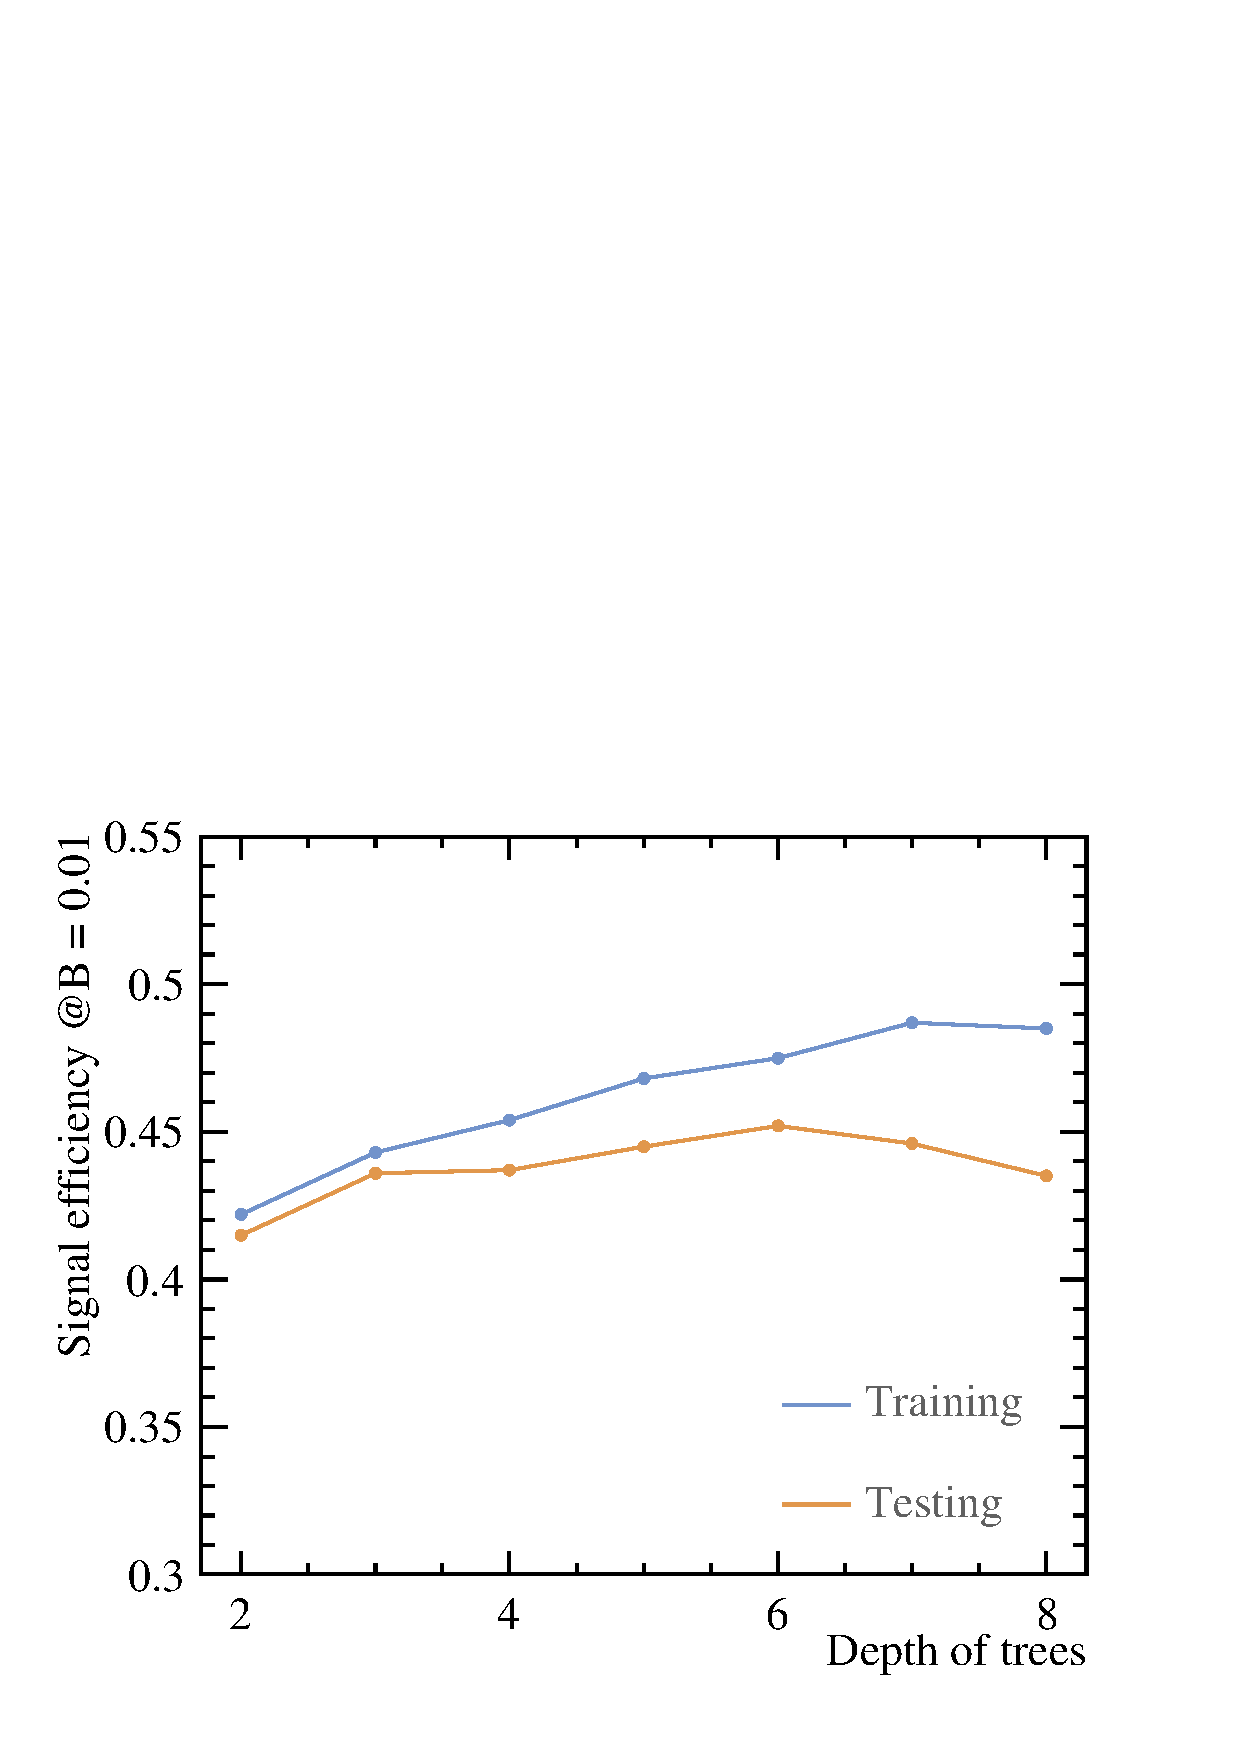
\includegraphics[width=0.45\textwidth]{doubleHiggs/DepthOfTrees.pdf}
\caption{Example of MVA overtraining}
\label{fig:doubleHiggsMVAovertraining}
\end{figure}

\FIGURE{fig:doubleHiggsMVAovertraining} shows a typical overfitting plot. Overfitting is defined when the efficiency of signal selection in the training samples increases, but the efficiency in the testing sample decreases. Here the example is chosen from double Higgs analysis at \rootS{3}, using Boosted Decision Tree model. The efficiency of signal selection is defined as the signal fraction when background fraction is 1\%, report by the TMVA training process. In \Figure{fig:doubleHiggsMVAovertraining} , the depth of the tree, or the number of layers in the tree, reflects the complexity of the model. From tree depth 2 to 5, the efficiency for both testing and training samples increases. From tree depth 6 onwards, the overfitting occurs. In this particular example, one should choose a tree depth fewer than 7 to avoid overfitting.

There are methods to assign the error on the selection efficiency. Thus one can make a better choice of parameters to avoid overfitting. These methods were not implemented due to the technical capacity provided by the TMVA.

\subsection{Choice of models}

The model, also known as the classifier in TMVA, can be as simple as cut based, likelihood or linear regression. It can also be as complicated as non linear tree, non linear neutral network or support vector machine. Regardless of model complexity, the choice of most optimal classifier is often data driven. Also, given the free parameters in each model, the comparison between different models without individual tuning is not rigourous. Nevertheless, as researchers in the machine learning suggested, the boosted decision tree is probably the best out-of-the-box machine learning method. Neutral network could potentially be better than the boosted decision, but it requires more tuning, and it is less intuitive to interpret the model. For these reasons, boost decision tree (BDT) is often the choice of machine learning model in the high energy physics. And it is used in various physics analysis in this document.

Before describing BDT in detail, we will first visit some simple models.

%the traditional rectangular cut model, and the Projective Likelihood method, which is used in the photon ID in the \pandora in \Section{}.



\subsubsection{Rectangular Cut}

Probably the most intuitive model, the rectangular cut method optimise cuts to maximise some specific metric. The metric could be the signal efficiency for a particular background efficiency. Alternatively, the metric can be the significance, $\frac{S}{\rootOf{S\!+\!B}}$, where $S$ and $B$ are signal and background numbers, respectively.

Discriminative variables gives better separation power when they are gaussian-like and statistically independent. Therefore it is common to decoorelate  the variables and gaussian transform them before using the rectangular cut MVA.

Because its simplicity, the cut method is often performed manually, much more often in the time pre-date the wide spread of machine learning methods. It is still commonly used for the pre-selection step before the MVA (see \Section{sec:doubleHiggsPreSelection}), and other simple cases. Unless specified, the optimal cuts proposed in this document for various physics analysis are found using the rectangular cut method manually.

\subsubsection{Projective Likelihood}

Projective likelihood model (PDE) is used in \pandora for the photon ID  due to its simplicity and low requirement on computing resources. It is discussed in details in \Section{sec:photonPDE}

\begin{comment}
\subsection{Projective Likelihood}

Projective likelihood model (PDE) is used in \pandora for the photon ID due to its simplicity and low requirement on computing resources.

PDE implemented in the TMVA calculates the probability density for each discriminative variable, for signal and background. The overall signal and background likelihood are defined as products of the individual probability density. The likelihood ratio, $R$, is then defined as the signal likelihood over signal plus background likelihood.

TMVA implementation also fits an underlying function to the probability density. The \pandora implementation simply uses binned likelihood ratio, $R$, as the output, due to the simplicity. The sub-categories for the \pandora implementation are determined by the cluster energy.

Similarly to the rectangular cut method, PDE works better with decorrelated, gaussian like variables. The \pandora implementation did not decorrelate nor transform the variables, to keep implementation fast.
\end{comment}

\subsubsection{Boosted decision tree}
\label{sec:analysisBDT}

Boost decision tree (BDT) is a non linear tree based model. Its rather complex nature requires a careful explanation of many concepts within the BDT.

\paragraph{Decision tree}
Decision tree is a binary tree, where each node, the splitting point, uses a single discriminative variable to decide whether a event is signal-like (``goes down by a layer to the left''), or background-like (``goes down by a layer to the right''). At each node, samples are divided into signal-like and background-like sub-samples. The tree growing starts at the root node, and stops at certain criterion, which could be the minimum number of events in a node, the number of layers of the tree, or a minimum/maximum signal purity.

The training of the decision tree is to determine the optimal cut at the node by minimising the metric. The probability of the cut producing the signal is $p$. Three commonly used metrics for two-class classification are
\begin{enumerate}
\item Misclassification error:  $1 - \max\parenths{p\!,\!1\!-\!p}$,
\item Gini index: $2p\parenths{1\!-\!p}$,
\item Cross-Entropy or deviance: $-p\log{p}-\parenths{1\!-\!p}\log\parenths{1\!-\!p}$.
\end{enumerate}

The using of a trained decision tree is to transverse along the tree. The event is classified as signal or background depending on whether it falls in the signal-like or background-like end node.

\begin{figure}[!tbp]
\includegraphics[width=0.45\textwidth]{doubleHiggs/mva/BDTcomic}
\caption{Example of a decision tree}
   \label{fig:doubleHiggsMVAdecisionTree}
\end{figure}

\FIGURE{fig:doubleHiggsMVAdecisionTree} illustrate a simple example of a decision tree. The signal is the PhD student and the background is the undergraduate student. The depth of this imbalance binary  tree is 2. A node is represented by a diamond.  The signal-like node is the red rectangle and the background-like nodes are blue rectangles. The tree is constructed with two possible cut, ``Party ends before 1am'' and ``Know where free pizza is''. The attribute of samples is listed in \Table{tab:doubleHiggsDecisionTreeComic}. To demonstrate the choice of the first layer cut, the Gini index metric is used. If the first cut is ``Party ends before 1am'', the probability of the cut producing the signal, $p$, is $\frac{10}{13}$. Gini index is $2p\parenths{1\!-\!p} \backsimeq 0.36 $. If the first cut is ``Know where free pizza is'', $p=\frac{10}{15}$. Gini index is $2p\parenths{1\!-\!p} \backsimeq 0.44 $. Therefore, the first cut is ``Party ends before 1am''.

The simple tree in \Figure{fig:doubleHiggsMVAdecisionTree} is grown fully as each end node contains signal or background only. To use the trained decision tree, if there is student who ends party before 1am and knows where free pizza is, then the student is classified as a PhD student.

\begin{table}[!tbp]\centering
\small
\begin{tabular}{lrr}
\hline \hline
Number & Party ends before 1am  & Know where free pizza is\\
\hline
PhD student & 10 & 10 \\
Undergrad student & 3 & 5 \\
\hline \hline
\end{tabular}
\caption
{The attribute of samples for the decision tree example.}
\label{tab:doubleHiggsDecisionTreeComic}
\end{table}

\paragraph{Improve decision tree}

Decision tree has a low bias, but high variance. This means it is very easy to construct a tree that fits the training data very well, but the tree would not be optimal for the testing sample. To overcome the instability of the decision tree, many methods have been developed. The most successful one is boosting.

Boosting: it is a technique where the misclassified events receives a higher weight than the correctly classified events. Therefore, when the training is iterated, the misclassified events would receive higher and higher wights and more likely to classify correctly. The boosting is done at every iteration, which can be few hundred or few thousand time. This will create a ``forest'' of many trees. The final output could be a majority vote, by transversing the event to the end node for each tree in the forest.

Bagging: also known as boot-strap, it is a method that select a simple random sub-set of the training sample, and apply the model. In this case, every boosting iteration takes a bagged sample, rather than the whole sample.

TMVA implementation of the BDT for the output is using a likelihood estimator, depending on how often a event is classified as signal in the forest. The likelihood number is later used to select signal from background.


\subsection{Optimisation of Boosted Decision Tree}

Many parameters of the BDT can be tuned. The tuned parameters are described below. The optimal values are obtained by choosing the best performance without overfitting with samples at \rootS{3}. The same values are used \rootS{1.4 analysis}.

The most important parameter is the depth of a tree, which determines how many end nodes a tree has, or the degrees of freedom of a tree. The related parameter is the number of trees. Experience shows that using many small trees yields the best result. The performance as a function of the depth is shown in \Figure{fig:doubleHiggsMVAovertraining}. The chosen value is 4.

The number of tree is another important parameter. Intuitively large number of trees leads to overfitting. However, it has been shown that a large number does not lead to overfitting, using the definition above. There is a debate on how to determine the optimal number of tree. The chosen value is 4000.

The minimum number of events in a node, which is a stopping criteria for tree growing, affects the size of the tree. But it is less influential than the depth of the tree. The chosen value is 0.25\% of the total events.

The boosting has two variant, adaptive boost and gradient boost. For all the BDT used in this document, adaptive boost is used.

The learning rate of the adaptive boost, which controls how fast the weight changes for events in each boosting iteration. Experience shows small learning rate with many trees work better than large learning rate with few trees. The chosen value is 05.

The usual choice of the metric for the optimal cuts is either Gini index or cross-entropy. Gini index metric is chosen. It makes little difference to performances, comparing to the cross-entropy metric.

Number of bins per variables for the cut is necessary to make tree growing efficient. Discrete binned variables are faster to computer than continuous variables. The parameter does not impact the performance much. However, variables should be pre-processed before going into the model. For example, the variable should be limited to a sensible range to avoid the extremes. The variable should also be transformed to obtain a more uniform distribution, if the original distribution is highly skewed. The chosen value is 40.

For the end node, it is determined as either signal-like or background-like, based on the majority for the training event in the end node. Numerically, it corresponds to 1/0. However, the end node could also use signal purity as the output, resulting in a continues spectrum of [0,1]. The chosen method is the continuous response.

\subsection{Multiple classes}
% ATTN used in tau chapter

The above discussion is done assuming two classes - signal and background. The argument can be easily extended to multiple classes. There are two ways for the training. "One v.s. one" is each class is trained against each other class. And the overall likelihood is normalised. The second way to train is called "one v.s. all", which is when each class is trained against all other classes.

Using a three-class example, A, B and C, "one v.s. one" scheme trains A against B, B against C, and C against A. Then the likelihood is normalised. "One v.s. all" would train A against B plus C, B against A plus C, and C against A plus B.

TMVA multiclass implementation uses "one v.s. all" scheme. Multiclass is used in falvour tagging of jets, \Section{sec:theoryFalvourTagging}, and in the tau lepton final state separation study, \Section{}.

\section{Event shape varaibles}

% ATTN used in tau chapter

Event shape variables are some useful global variables to describe the shape of the event, for example whether it is back-to-back, or homogenous in the solid angle.

The classical event shape thrust\cite{PhysRevLett.39.1587}, is defined as
\begin{equation}
T = \max_{\hat{t}}\!\frac{\sum_{i}\absOf{\hat{t}\!\cdot\!\vec{p_{i}}}}{\sum_{i}\absOf{\vec{p_{i}}}}
\end{equation}
where $\vec{p_{i}}$ is the momentum vector of the particle $i$. Summation is over all particles in the event. Thrust axis, $\hat{t}$, is a unit vector. (Principle) Thrust value, $T$, is 1 for a perfect pencillike back-to-back two-jet event, and 0.5 for a perfect spherical event. The thrust value is useful in picking out back-to-back two-jet event. Thrust axis is useful to separate each jet in a back-to-back two-jet event.

It is  derived from the sphericity tensor \cite{PhysRevLett.35.1609}, defined as
\begin{equation}
\bm{S^{\alpha\beta}} = \frac{\sum_{i}p^{\alpha}_{i}p^{\beta}_{i}}{\sum_{i}\absOf{\vec{p_{i}}}^2},
\end{equation}
where $\vec{p_{i}}$ is the momentum vector of the particle $i$. Summation is over all particles in the event. $\alpha$ and $\beta$ refer to the x, y, z coordinate axis. Eigenvalues of tensor $\bm{S}$ can be found, or in this case diagonalisation of the matrix $\bm{S}$, denoted with $\lambda_{1}$, $\lambda_{2}$, $\lambda_{3}$. The normalisation condition requires $\lambda_{1}\!\geqslant\! \lambda_{2} \! \geqslant \! \lambda_{3}$ and $ \lambda_{1} \! + \! \lambda_{2} \! + \! \lambda_{3} \! = \! 1 $. Sphericity, $S$, is defined in terms of $\lambda$,
\begin{equation}
\sphericity = \frac{3}{2}\parenths{\lambda_{1} \! + \! \lambda_{2}}.
\end{equation}
\sphericity, is 0 for a perfect pencil-like back-to-back two-jet event, and 1 for a perfect spherically symmetric event.

Sphericity tensor \cite{PhysRevLett.35.1609}, is defined as
\begin{equation}
\bm{S^{\alpha\beta}} = \frac{\sum_{i}p^{\alpha}_{i}p^{\beta}_{i}}{\sum_{i}\absOf{\vec{p_{i}}}^2},
\end{equation}
where $\vec{p_{i}}$ is the momentum vector of the particle $i$. Summation is over all particles in the event. $\alpha$ and $\beta$ refer to the x, y, z coordinate axis. Eigenvalues of tensor $\bm{S}$ can be found, or in this case diagonalisation of the matrix $\bm{S}$, denoted with $\lambda_{1}$, $\lambda_{2}$, $\lambda_{3}$. The normalisation condition requires $\lambda_{1}\!\geqslant\! \lambda_{2} \! \geqslant \! \lambda_{3}$ and $ \lambda_{1} \! + \! \lambda_{2} \! + \! \lambda_{3} \! = \! 1 $. Sphericity, $S$, is defined in terms of $\lambda$,
\begin{equation}
S = \frac{3}{2}\parenths{\lambda_{1} \! + \! \lambda_{2}}.
\end{equation}
$S$, is 0 for a perfect pencillike back-to-back two-jet event, and 1 for a perfect spherically symmetric event.

Aplanarity is another event shape varaible that distinguishes spherical symmetrical events from planar and linear events. The definition is
\begin{equation}
S = \frac{3}{2}\parenths{\lambda_{1}},
\end{equation}
where $\lambda_{1}$ is the largest eigenvalue in the diagonalised sphericity tensor.

\section{Miscellaneous}

An event in a collider experiment refers to one collision and the subsequent energy deposition in the detector. An event corresponds to a certain type of physics process.

Often we are dealing with extracting a type of events, from a large number of other events. The signal, or signal events refer to events of interests. Other events are referred to as the background, or background events.

Typical metrics of signal selection is efficiency and purity. This toy example illustrates definitions of efficiency and purity.

\begin{table}[!tbp]
\begin{tabular}{lrr}
\hline
\hline
Event Number  &  True Signal & True Background  \\
\hline
Selected Signal & $N_S$ & $N_1$ \\
Selected Background & $N_2$ & $N_B$ \\
\hline
\hline

\end{tabular}
\caption[A toy example to demonstrate definitions of efficiency and purity.]%
    {A toy example to demonstrate definitions of efficiency and purity.}
\label{tab:analysisToyExample}
\end{table}
Signal selection efficiency is defined as $\frac{N_S}{N_S \! + \! N_2}$. Signal selection purity is defined as $\frac{N_S}{N_S \! + \! N_1}$.
Significance is a quantity that is similar to purity, $\frac{N_S}{\rootOf{N_S \! + \! N_1}}$

When we are describing particles, light lepton, \llight, refer to electrons, \Pem, and muons, \Pmuon. Light quarks, \qlight, refer to up quark, \Pup, down quark, \Pdown, and strange quark, \Pstrange.

Computational intensive jobs are processed either on the Cambridge High Energy Physics grid, or the \CLIC computing grid.
%Thanks computing resources. i.e. ILC VO, CLIC grid, etc. 
  \chapter{Photon Reconstruction in PandoraPFA}
\label{chap:Reconstruction}

\chapterquote{Photons have mass? I didn��t even know they were Catholic.}%
{Woody Allen}

\section{Introduction}

Why photon reconstruction important.

\begin{comment}


Since the discovery of a particle consistent with being the SM Higgs boson in LHC at 2012 \cite{Aad:2012tfa,Chatrchyan:2012ufa}, our understanding of Standard Model has improved greatly. Yet limited by the underlying QCD interaction from proton-anti-proton collision, one has great difficulty to measure the properties of the Higgs precisely. Next generation electron-positron linear collider could hopefully make precision measurements of the Higgs sector and the Top quark sector \cite{Abramowicz:2013tzc}.

The leading candidates for next generation electron-positron linear collider are the International Linear Collider (ILC) \cite{Brau:2007zza}, and the Compact Linear Collider (CLIC) \cite{Linssen:2012hp}. The ILC has developed two detector models, namely the International Large Detector (ILD) \cite{Abe:2010aa} and the Silicon Detector (SiD) \cite{Aihara:2010zz}. The CLIC has developed two slightly modified detector models based on ILD and SiD \cite{Linssen:2012hp}. One key common feature of these next generation electron-positron linear colliders is the high granular calorimeter, which provides a great spatial resolution at the cost of the energy resolution. Particle flow algorithms (PFA) benefit from the spatial resolution from calorimeters, together with tracking information, to provide excellent a jet energy resolution. PandoraPFA, the most complicated and the best performing one, provides a jet energy resolution of less than 3.5\%, which is required for W/Z separation \cite{Thomson:2009rp,Marshall:2013bda}.

\begin{figure}[tbph]
\centering
{\includegraphics[width=0.5\textwidth]{images/tautauMod}}%

\caption{An event display of a simulated $\Pem\Pep\to \Ptauon\APtauon$ event. The blue region is the cross section of the Electromagnetic Calorimeter barrel region. The top $\Ptau$ decays into a charged $\Ppi$, two photons and neutrinos. The bottom $\Ptau$ decays into a muon and neutrinos.}
\label{fig:Tautau}
\end{figure}

Photon reconstruction is an important part of particle reconstruction. For many physics processes involving particles decaying into photons, such as $\Ptau$ lepton and $\Ppizero$, a good photon reconstruction, which provides a good single photon completeness and purity, as well as a good photon separation resolution, is crucial for reconstructing these particles.

\end{comment}
\section{Overview of photon reconstruction in PandoraPFA}

PandoraPFA provides a framework for particle reconstruction \cite{}, as described in \Section{}. In the linear collider content, it has a vast library of algorithms developed through years by many people. Each algorithm addresses one topological issue in the particle reconstruction \cite{}. The essential part of the PandoraPFA is track-cluster association and reclustering to find the best track-cluster pair. Algorithms that removes trackless clusters, such as removing muon clusters or photon clusters, would provide a clean environment for the track-cluster association, hence improving the jet energy resolution.

Photon identification in the PandoraPFA has two main mechanisms. The basic mechanism tests trackless clusters, the after track-cluster association and the reclustering processes. The second more sophisticated photon identification is performed before the track-cluster association and reclustering process. This algorithm identifies photon electromagnetic shower cores carefully in the dense jet environment.

Second mechanism improves jet energy resolution by correctly identifying photon electromagnetic shower cores and leaving a cleaner environment for the track-cluster association. However, the peripheral calorimeter hits to the shower cores may be left as fragments, and reconstructed as separate particles. This lowers the reconstructed photon completeness and makes the number of reconstructed photons a less useful physical quantity. Also, the second mechanism leaves rooms for improvement of photon separation resolution, illustrated in \Figure{}.

This section presents a solution to the photon fragments issue. The introduced PandoraPFA algorithms also improves the photon separation resolution. Algorithms related to photon reconstruction, fragmental removal and photon splitting, which are written or introduced by authors, will be discussed below.

%Three algorithm will be discussed: a rewritten sophisticated photon reconstruction algorithm, a photon fragment removal algorithm and a photons splitting algorithm.

%The testing simulated data in this paper are generated either by WHIZARD \cite{whizard} or by the simple HepEvt generator. Events are simulated with GEANT4 \cite{Agostinelli:2002hh} in MOKKA \cite{MoradeFreitas:2002kj}. Jet fragmentation was performed with PYTHIA \cite{Sjostrand:1995iq} and the particle reconstruction was done by PandoraPFA \cite{Marshall:2015rfa} in MARLIN reconstruction framework \cite{Gaede:2006pj}, in ILD\_o1\_v6 detector model. The iLCSoft v17-01-07 was used. Different versions of PandoraPFA were used for the comparison purpose.

\section{Overview of photon reconstruction algorithm}
\label{sec:photonRecostrcution}
The photon reconstruction algorithm refers to the more sophisticated photon identification of the two main identification mechanisms, before the track-cluster association and reclustering process. The algorithm has the following steps: coarsely forming photon clusters, reconstructing photon candidate, photon ID test, and optional fragment removals.

\subsection{Form photon clusters}

This step finds large potential photon clusters. All calorimeter hits in the \ECAL, which are not used in previous algorithms, are grouped into clusters using a cone based clustering algorithm. To find photon clusters, which do not deposit energies in the tracking system, the cone clustering algorithm is seeded with energetic hits. The parameters for the cone clustering are generous, allowing potentially two or three photons in one cluster.

\subsection{Reconstruct photon candidates}
\label{sec:photonCandiate}

The large photon clusters are split into smaller photon candidates, using two-dimensional shower profiles. The candidates close to a track projection are deemed as non-photons. Identifying photon candidates within a large photon cluster relies on the characteristic electromagnetic showers, in particular the transverse distribution. A energetic photon or electron hits the absorber layers of the \ECAL, it initiates an electromagnetic shower, where electron pair production and bremsstrahlung produce more low-energy photons and electrons. The transverse distribution is characterised by a narrow cone, widening while the shower develops.

To view the transverse shower distribution, a two-dimensional energy deposition projection is constructed in the plane perpendicular to the direction of the cluster. \Figure{fig:photonPeakFinding} shows the energy deposition projection of two photons candidates. U and V axis are two arbitrary orthogonal axis in the transverse plane perpendicular to the direction of photons. Z axis shows the sum of the calorimeter hit energy in GeV. The bin size corresponds to the square \ECAL cell size.

\begin{figure}[tbph]
\centering
{\includegraphics[width=0.5\textwidth]{photon/peakFinding}}%

\caption{Two 500\,GeV photons (yellow and blue), just resolved in the transverse plane perpendicular to the direction of the flight, of their energy deposition in electromagnetic calorimeter. U and V axis are two arbitrary axis perpendicular to each other in the plane. Z axis is the sum of the calorimeter hit energy in each particular bin in 2D plane in GeV.}
\label{fig:photonPeakFinding}
\end{figure}

By using the two-dimensional energy deposition projection, separating photons translates to separating peaks in the projection. Therefore a high performance two dimensional peak finding algorithm is the key to identify multiple photons. The peak finding algorithm will be discussed in \Section{sec:peakFinding}

The output of this step is a collection of photon candidates from a photon cluster, which will be fed to the photon ID test.

\subsection{Photon ID test}
\label{sec:photonIDtest}

Photon ID test decides if a a candidate is a photon. If a candidate is not a photon, the calorimeter hits of the candidate will be passed on to the next stage of the reconstruction.  The photon ID test is a multidimensional likelihood classifier. The classifier is trained with discriminating variables, which exploit features electromagnetic showers. The classifier will be discussed in \Section{}

\subsection{Photon Fragment removal}
\label{sec:photonRecoFragRemoval}
The optional photon fragment removal aims to merge small photon fragment to main photons. Since this step shares the same logic as the algorithm in \Section{}, only differing in the cut-off values for merging metrics, this step be discussed in \Section{}.

This step marks the end of the photon reconstruction algorithm. The output are a collection of reconstructed photons, separated from non-photon calorimeter hits.
%The candidate passed the test will be kept in a separate container for photons only

\section{Two dimensional peaking find algorithm for photon candidate}
\label{sec:peakFinding}

As discussed in \Section{sec:photonCandiate}, separating photon candidates from a cluster is same as identifying peaks in a two dimensional histogram. An example of two photons is shown in the \Figure{fig:photonPeakFinding}. The basic algorithm treats all clusters as potential photon clusters. Since charged hadrons would deposit tracks in the tracking system, extra care is taken when a cluster is close to the projection of the track in the front of the \ECAL. The basic peak finding algorithm has two main functions: identifying peaks, and assigning bins to peaks.

A local peak is defined as a bin where its height is above all eight neighbouring bins. After all peak bins are found, non-peak bins are associated to one peak bin, by choosing the peak bin that minimise the metric
\begin{equation}
\frac{d}{\sqrt{E_{peak}}}
\end{equation}
where $d$ is the Euclidean distance between a non-peak bin and a peak bin, and $E_{peak}$ is the energy or the height of the peak bin. Alternative metrics provided in the algorithm include $d$, $\frac{d}{{E_{peak}}}$, and $\frac{d}{{E_{peak}^2}}$. The default metric is chosen due to a good balance between distance and energy of the peak.

\subsection{Candidate close to track projection}

If a cluster or a photon candidate is close to the projection of the track in the front of the \ECAL, it is likely that the cluster or the candidate is a charged hadron. Misidentifying a charged hadron as a photon leads to significant degradation in reconstruction performance. However, if a photon next to a charged hadron is carefully reconstructed, the overall reconstruction is improved. Hence this step aims to carefully identifies photon candidate next to charged hadrons, by using track information and features of the electromagnetic shower. Photon induced electromagnetic shower in the \ECAL typically start in the first few layers. As the shower develops, the direction of the shower core does not change much.

If a peak bin is within the eight neighbouring bins of the track projection onto the two dimensional plane, the peak and its associated bins are flagged as non-photons. Furthermore, the \ECAL is sliced longitudinally to help identify photon candidates. For example, the default three slices will result in three \ECAL fiducial spaces, each contains space from the front of the \ECAL to a third, two thirds and the back of the \ECAL, respectively. The peaking finding algorithm is repeated for the same cluster divided in each \ECAL fiducial space. The peak is only preserved as a photon candidate if the peak exists in every fiducial space, and if its position is shifted by no more than one neighbouring bin between fiducial spaces.


\subsection{Peak filtering}

The performance of the two dimensional peaking finding algorithm is improved by clever programming and physics arguments. For a given two dimensional histogram, such as the one in \Figure{fig:photonPeakFinding}, major peaks most likely correspond to physical photons, while the minor peaks more likely come from fluctuations in energy deposition. To select major peaks, every time after non-peak bins are associated with peak bins, minor peaks with fewer than three bins associated (including the peak bin) are discarded. These bins are then associated with non-discarded peaks.  The algorithm also allows bins with height below a critical value to not participate in the peak finding. The default value is set such that only empty bins are not used.

\subsection{Inclusive mode}
\label{sec:photonPeakFindingInclusive}

The two dimensional histogram is iterated a few times during the algorithm. The time complexity is $O(n^2)$ for a $n \times n$ histogram (Default $n = 41$). Therefore, for the purpose of speed, it is undesirable to have a very large histogram. However, since the histogram has a finite size, only energy deposition projected on the histogram would be considered for peak finding.  This behaviour is suitable for photon reconstruction (\Section{sec:photonCandiate}) and test for photon fragment removal (\Section{sec:photonFragRemoval}). However, for photon splitting (\Section{sec:photonSplitting}), there should be no calorimeter hits loss from splitting a photon. Hence inclusive mode of the peak finding algorithm is developed, and it allows energy deposition projected outside the histogram to be associated with identified peaks.


\section{Likelihood classifier for photon ID}
\SECTION{sec:photonLikelihood}

\SECTION{sec:photonIDtest} outlines the photon ID test in the photon reconstruction algorithm. This section describes the multidimensional likelihood classifier in details, including discriminating variables. For each photon candidate, a set of kinematic variables are calculated. The classifier training typically uses simulated jet events.


%Photon ID test decides if a a candidate is a photon. If a candidate is not a photon, the calorimeter hits of the candidate will be passed on to the next stage of the reconstruction.  The photon ID test is a multidimensional likelihood classifier. The classifier is trained with discriminating variables, which exploit features electromagnetic showers. The classifier will be discussed in \Section{}


Kinematic variables exploit the differences between a characteristic electromagnetic shower and a hadronic shower, and the fact that a photon is more likely to be isolated from other showers and charged tracks. Two variables use the longitudinal shower distribution: the first \ECAL layer of the shower, and the difference between a expected longitudinal distribution and the observed. Two variable uses the transverse shower distribution: in the transverse plane with two orthogonal axes, the r.m.s. distance of associated bins to the peak bin, and the smallest ratio of the two r.m.s. distances in each axis direction. One variable is the ratio between the photon candidate energy to the photon cluster energy. The last kinematic variable is the distance between the photon candidate and the closest track projection. The distributions of kinematic variables are normalised to probability distribution, stored in binned histograms.


Furthermore, the classifier is improved by realising the kinematic variable distributions depend on the photon energy. Thus these distributions are divided by bins of photon candidate energy. The numbers of photon and non-photon candidates in each energy bin are also different, which helps the ID test. The default energy bins edges are 0.2, 0.5, 1, 1.5, 2.5, 5, 10, 20\,GeV, which covers a good range of photon energies. Candidate with energy below 0.2\,GeV would not be examined in this step, as it is very unlikely to be a photon.
%Beyond 20\,GeV, most candidates are photon candidate.

For a given candidate, which falls in a energy bin, the likelihood classifier output is given by

\begin{equation}
pid = \frac{N\prod{P_i}}{N\prod{P_i} + N'\prod{P'_i}}
\end{equation}
where $P_i$ and $P'_i$ are the probability of $i^{th}$ kinematic variable of photon and non-photon candidates. $N$ and $N'$ are the number photon and non-photon candidates. These are obtained during classifier training.

During classification, a candidate passes the photon id test if
\begin{equation}
\begin{cases}
  pid > 0.6, & \text{if}\ 0.2 < E < 0.5\,GeV\\
  pid > 0.4, & \text{if}\ E \geqslant 0.5\,GeV
\end{cases}
\end{equation}
where $E$ is the candidate energy. Two values of the $pid$ cuts reflect the confidence of the id test with different candidate energy. The test is more cautious with low energy candidate.

\section{Overview of photon fragment removal algorithm}
\label{sec:photonFragRemoval}
During the reconstruction, it is possible that a core of the photon electromagnetic shower is identified as a photon (the main photon). The outer part of the shower is reconstructed as a separate particle, and wrongly identified as a photon or a neural hadron (the photon/neutral fragment). \Figure{fig:photonEvtDspPhotonFrag} shows a typical creation of such a photon fragment. The fragment does not have the electromagnetic shower structure, and typically it is has much lower energy than the main photon. If a photon-fragment pair is merged, the pair should be consistent with a one-particle profile. These characteristics are used to merge fragments to main photons.

\begin{figure}[tbph]
\centering

  \begin{subfigure}[b]{0.3\textwidth}
    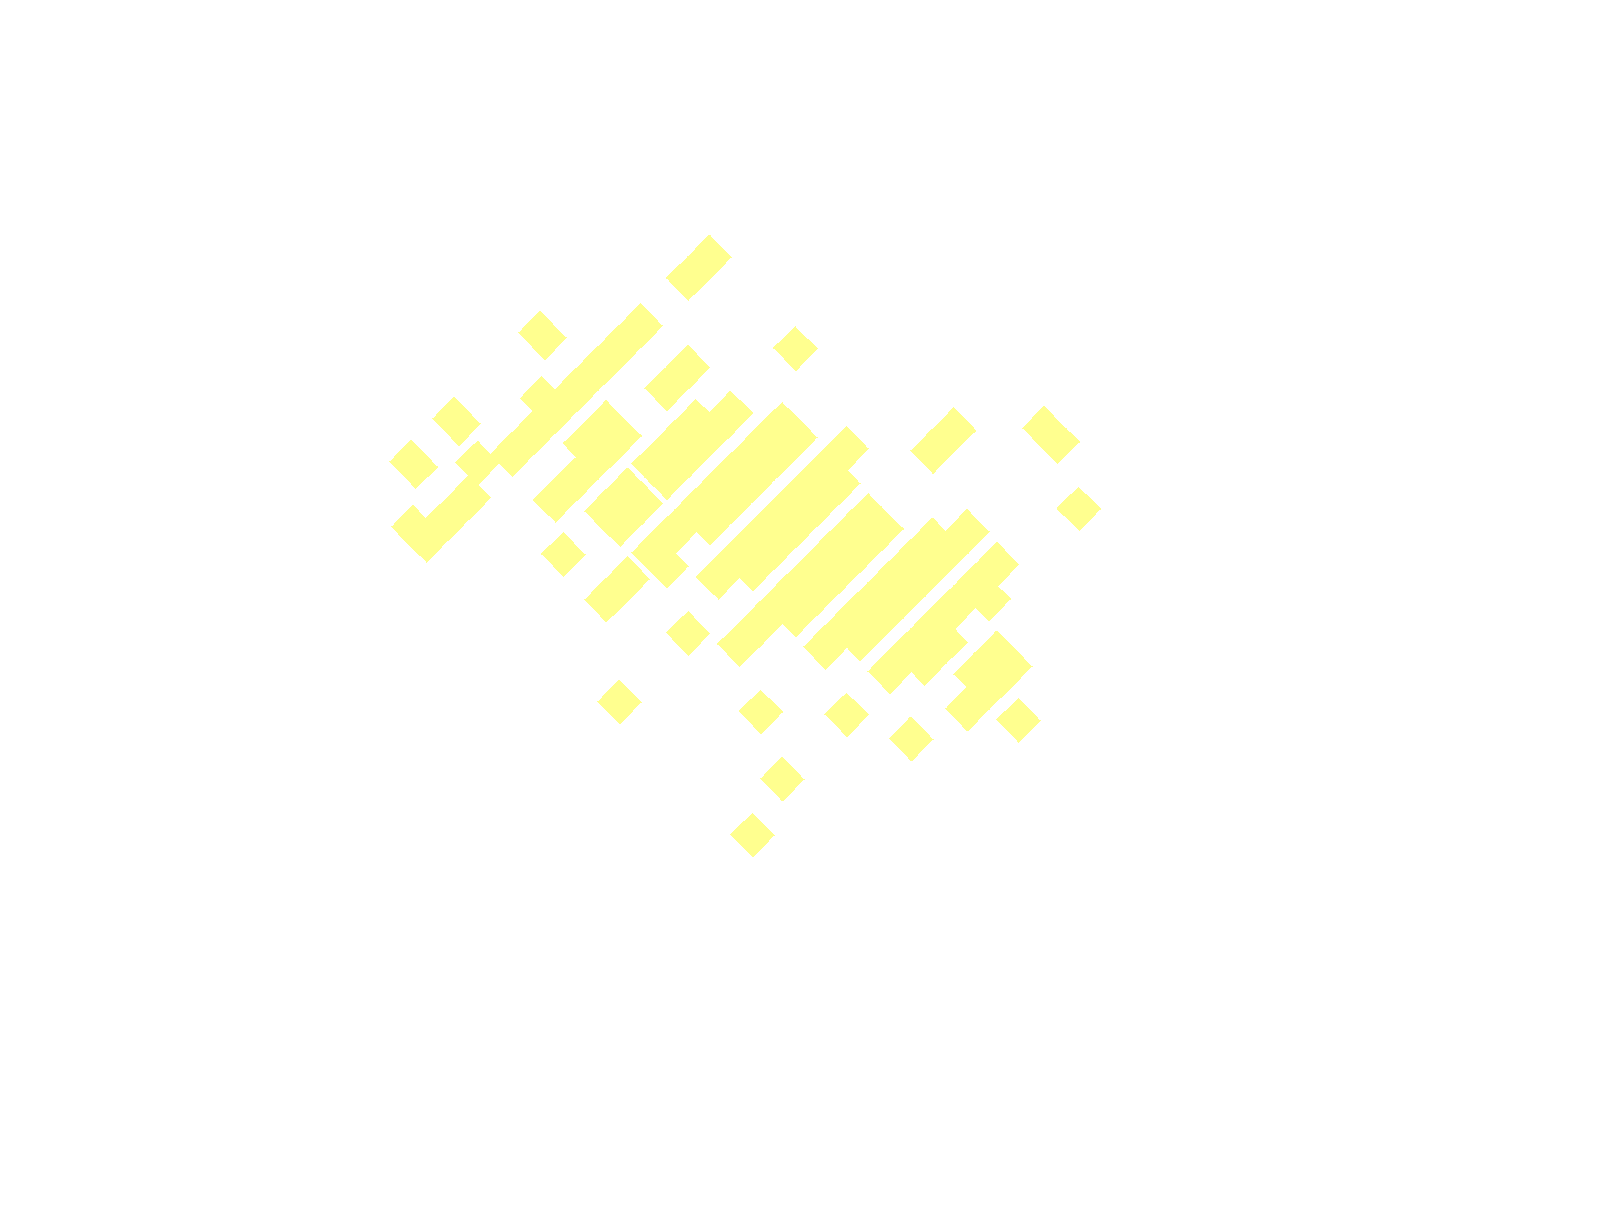
\includegraphics[width=\textwidth]{photon/allPhoton}
    \caption{}
    \label{fig:photonEvtDspPhotonFragAll}
  \end{subfigure}
  \begin{subfigure}[b]{0.3\textwidth}
    \includegraphics[width=\textwidth]{photon/big}
    \caption{}
    \label{fig:photonEvtDspPhotonFragBig}
  \end{subfigure}
  \begin{subfigure}[b]{0.3\textwidth}
    
\includegraphics[width=\textwidth]{photon/small}
    \caption{}
    \label{fig:photonEvtDspPhotonFragSmall}
  \end{subfigure}

\caption[]
{An event display of a typical 10\,GeV photon (\Figure{fig:photonEvtDspPhotonFragAll}), reconstructed into a main photon (\Figure{fig:photonEvtDspPhotonFragBig}) and a photon fragment (\Figure{fig:photonEvtDspPhotonFragSmall}). }
\label{fig:photonEvtDspPhotonFrag}
\end{figure}


Photon fragment removal algorithms can exist in multiple step in the reconstruction, at the end of the photon reconstruction (see \SECTION{sec:photonRecoFragRemoval}), or at the end of the reconstruction. Since these algorithms share the same base class, the latter one will be discussed. The former differs mostly in the default cut-off values for merging metrics.


A photon and a potential fragment form a pair of particles (photon-fragment pair), if they are spatially close. Kinematic and topological properties of the photon-fragment pair are examined. The pair is merged when the properties pass a set of cuts, developed by comparing true photon-fragment pairs and non photon-fragment pair. This merging test is iterated over all possible  photon-fragment pairs. If multiple photon-fragment pairs pass the merging test, the pair with closest distance metric, $d$, will be merged.

The photon-fragment pairs is classified into photon-photon-fragment pairs and photon-neutral-hadron-fragment pairs, because they have different kinematic and topological distributions. The pairs are further classified into low energy and high energy pair, depending on whether the fragment energy ($E_p$) above 1\,GeV. The cuts for merging pairs, are classified which will be explained later, are listed in \Table{tab:photonFragRemovalCuts}.

\begin{table}[htbp]
\centering

\smallskip
\small
\begin{tabular}{l  r  r }
\hline
Low $E_f$ &  Photon-photon & Photon-neutral-hadron \\
\hline
\multicolumn{1}{L{0.3\textwidth}}{transverse shower comparison} & \multicolumn{1}{R{0.3\textwidth}}{$d < 30 $, $\frac{E_{p1}}{E_m + E_f} > 0.9 $, $\frac{E_{p2}}{E_f} < 0.5 $, $E_{p1} > E_m$}  & \multicolumn{1}{R{0.3\textwidth}}{-} \\
\multicolumn{1}{L{0.3\textwidth}}{close proximity} & \multicolumn{1}{R{0.3\textwidth}}{-}  & \multicolumn{1}{R{0.3\textwidth}}{$d < 20 $, $d_c < 40 $} \\
\multicolumn{1}{L{0.3\textwidth}}{low energy fragment} & \multicolumn{1}{R{0.3\textwidth}}{$d < 20 $, $E_p < 0.4 $}  & \multicolumn{1}{R{0.3\textwidth}}{-} \\
\multicolumn{1}{L{0.3\textwidth}}{small fragment 1} & \multicolumn{1}{R{0.3\textwidth}}{$d < 30 $, $N_{calo} < 40 $, $d_c < 50 $}  & \multicolumn{1}{R{0.3\textwidth}}{$d < 50 $, $N_{calo} < 10 $, $d_h < 50$} \\
\multicolumn{1}{L{0.3\textwidth}}{small fragment 2} & \multicolumn{1}{R{0.3\textwidth}}{$d < 50 $, $N_{calo} < 20 $}  & \multicolumn{1}{R{0.3\textwidth}}{-} \\
\multicolumn{1}{L{0.3\textwidth}}{small fragment forward region} & \multicolumn{1}{R{0.3\textwidth}}{$N_{calo} < 40$, $d_c < 60$, $E_f < 0.6$, $\absCosTheta > 0.7$}  & \multicolumn{1}{R{0.3\textwidth}}{-} \\
\multicolumn{1}{L{0.3\textwidth}}{relative low energy fragment} & \multicolumn{1}{R{0.3\textwidth}}{$d < 40$, $d_h < 20$, $\frac{E_{f}}{E_m} < 0.01$}  & \multicolumn{1}{R{0.3\textwidth}}{$d < 40$, $d_h < 15$, $\frac{E_{f}}{E_m} < 0.01$} \\
\hline
High $E_f$ &  Photon-photon & Photon-neutral-hadron \\
\hline
\multicolumn{1}{L{0.3\textwidth}}{transverse shower comparison} & \multicolumn{1}{R{0.3\textwidth}}{$\frac{E_{p1}}{E_m + E_f} > 0.9 $, $E_{p2} = 0$ or ($\frac{E_{p2}}{E_f} < 0.5 $, $E_{p1} > E_m$)}  & \multicolumn{1}{R{0.3\textwidth}}{$\frac{E_{p1}}{E_m + E_f} > 0.9 $, $E_{p2} = 0$ or ($\frac{E_{p2}}{E_f} < 0.5 $, $E_{p1} > E_m$)} \\
\multicolumn{1}{L{0.3\textwidth}}{relative low energy fragment 1} & \multicolumn{1}{R{0.3\textwidth}}{$d < 40$, $d_h < 20$, $\frac{E_f}{E_m} < 0.02$} & \multicolumn{1}{R{0.3\textwidth}}{$d < 40$, $d_h < 20$, $\frac{E_f}{E_m} < 0.02$} \\
\multicolumn{1}{L{0.3\textwidth}}{relative low energy fragment 2} & \multicolumn{1}{R{0.3\textwidth}}{-}  & \multicolumn{1}{R{0.3\textwidth}}{$d < 40$, $d_h < 20$, $\frac{E_f}{E_m} < 0.1$, $E_f > 10$} \\
\multicolumn{1}{L{0.3\textwidth}}{relative low energy fragment 3} & \multicolumn{1}{R{0.3\textwidth}}{-}  & \multicolumn{1}{R{0.3\textwidth}}{$d < 20$, $d_h < 20$, $\frac{E_f}{E_m} < 0.2$, $E_f > 10$} \\
\hline

\hline
\end{tabular}

\caption[]%
{The cuts for merging photon-photon-fragment pairs and photon-neutral-hadron-fragment pairs for both low energy and high energy fragments. $d$, $d_c$ and $d_h$ are the mean energy weighted intra-layer distance of the pair, the distance between centroids, the minimum distance between calorimeter hits of the pair. $E_m$ and $E_f$ are the main photon energy and the fragment energy. $E_{p1}$ and $E_{p2}$ are the two largest peaks, found by peak finding algorithm, ordered by descending energy. $N_{calo}$ is the number of the calorimeter hits in the fragment. $\absCosTheta$ is the absolute cosine of the polar angle, where beam direction is the z-axis.}
\label{tab:photonFragRemovalCuts}
\end{table}

\TABLE{tab:photonFragRemovalCuts} lists cuts for merging photon-photon-fragment pairs and photon-neutral-hadron-fragment pairs for both low energy and high energy fragments. $d$, $d_c$ and $d_h$ are the mean energy weighted intra-layer distance between  each \PFO in the pair, the distance between centroids, the minimum distance between calorimeter hits of each \PFO in the pair, respectively. $E_m$ and $E_f$ are the main photon energy and the fragment energy. $E_{p1}$ and $E_{p2}$ are the two largest peaks and associated calorimeter hits, found by the two dimensional peak finding algorithm (\Section{sec:peakFinding}), ordered by descending energy, using the pair as input. $N_{calo}$ is the number of the \ECAL hits in the fragment. $\absCosTheta$ is the absolute cosine of the polar angle of the main photon, where beam direction is the z-axis.

Three distance measurements have subtle difference. $d_c$ gives the distance between centroids of each \PFO in the pair, which is a quick but crude measurement. $d_h$ is the minimum distance between calorimeter hits of each \PFO in the pair. For a true photon-fragment, $d_h$ should be close to zero as the pair should be spatially close. $d$ is the mean energy weighted intra-layer distance between  each \PFO in the pair:
\begin{equation}
d = \frac{\sum_{i}^{layers}d_{l,i}\ E_{f,i}}{\sum_{i}^{layers}E_{f,i}}
\end{equation}
where $i$ indicates $i^{th}$ pseudo-layer of the \ECAL. $d_{l,i}$ is the minimum distance between calorimeter hits of the pair in the $i^{th}$ pseudo-layer. $E_{f,i}$ is the energy of the fragment in the the $i^{th}$ pseudo-layer. $d$ is a better measurement of the closeness of the pair. Similar to $d_h$, $d$ will be very small for a true photon-fragment pair.

One logic for merging is when the fragment is small with low energy and is close to the main photon. The other logic is when the pair looks like one photon in two-dimensional energy deposition projection (see \Section{sec:photonCandiate} and \Figure{fig:photonPeakFinding}). Comparing low $E_f$ and high $E_f$ cut, the cuts are similar. High $E_f$ cuts are more relaxed on the energy comparison for small fragment test. Comparing photon-photon-fragment pair and photon-neutral-hadron-pair, cuts for photon-neutral-hadron-pair are more conservative for low $E_f$, but more relaxed for high $E_f$. This reflects that the neutral hadron fragments originated from charged particles are more likely to be low energy.


Since all possible photon-fragment pairs are compared, this is a costly cooperation with $O(n^2)$ time complexity for $n$ particles. The speed is improved by considering only the pairs with $d<80\text{mm}$. The algorithm occurs at the end of the reconstruction.


\section{High energy photon fragment recovery algorithm}

\SECTION{sec:photonFragRemoval} descried effective algorithms to removal photon fragments that are peripheral to the main photon, or the electromagnetic shower core. An example of such fragment is shown in \Figure{fig:photonEvtDspPhotonFrag}. There is another type of fragment which is the leakage effect of the \ECAL. When the high energy photon shower is not fully contained in the \ECAL, shower deposits energy in the \HCAL, which often forms a neutral hadron in the \HCAL. Photon reconstruction, as described in \Section{sec:photonRecostrcution}, considers only calorimeter hits in the \ECAL.  An example of a 500\,GeV photon reconstructed into a main photon in the \ECAL (yellow) and a neutral hadron fragment in the \HCAL (blue) is shown in \Figure{fig:photonEvtDspHCalFrag}. For the \ILD detector, this \ECAL leakage effect appears when the photon energy is above 50\,GeV.





\begin{figure}[tbph]
\centering
{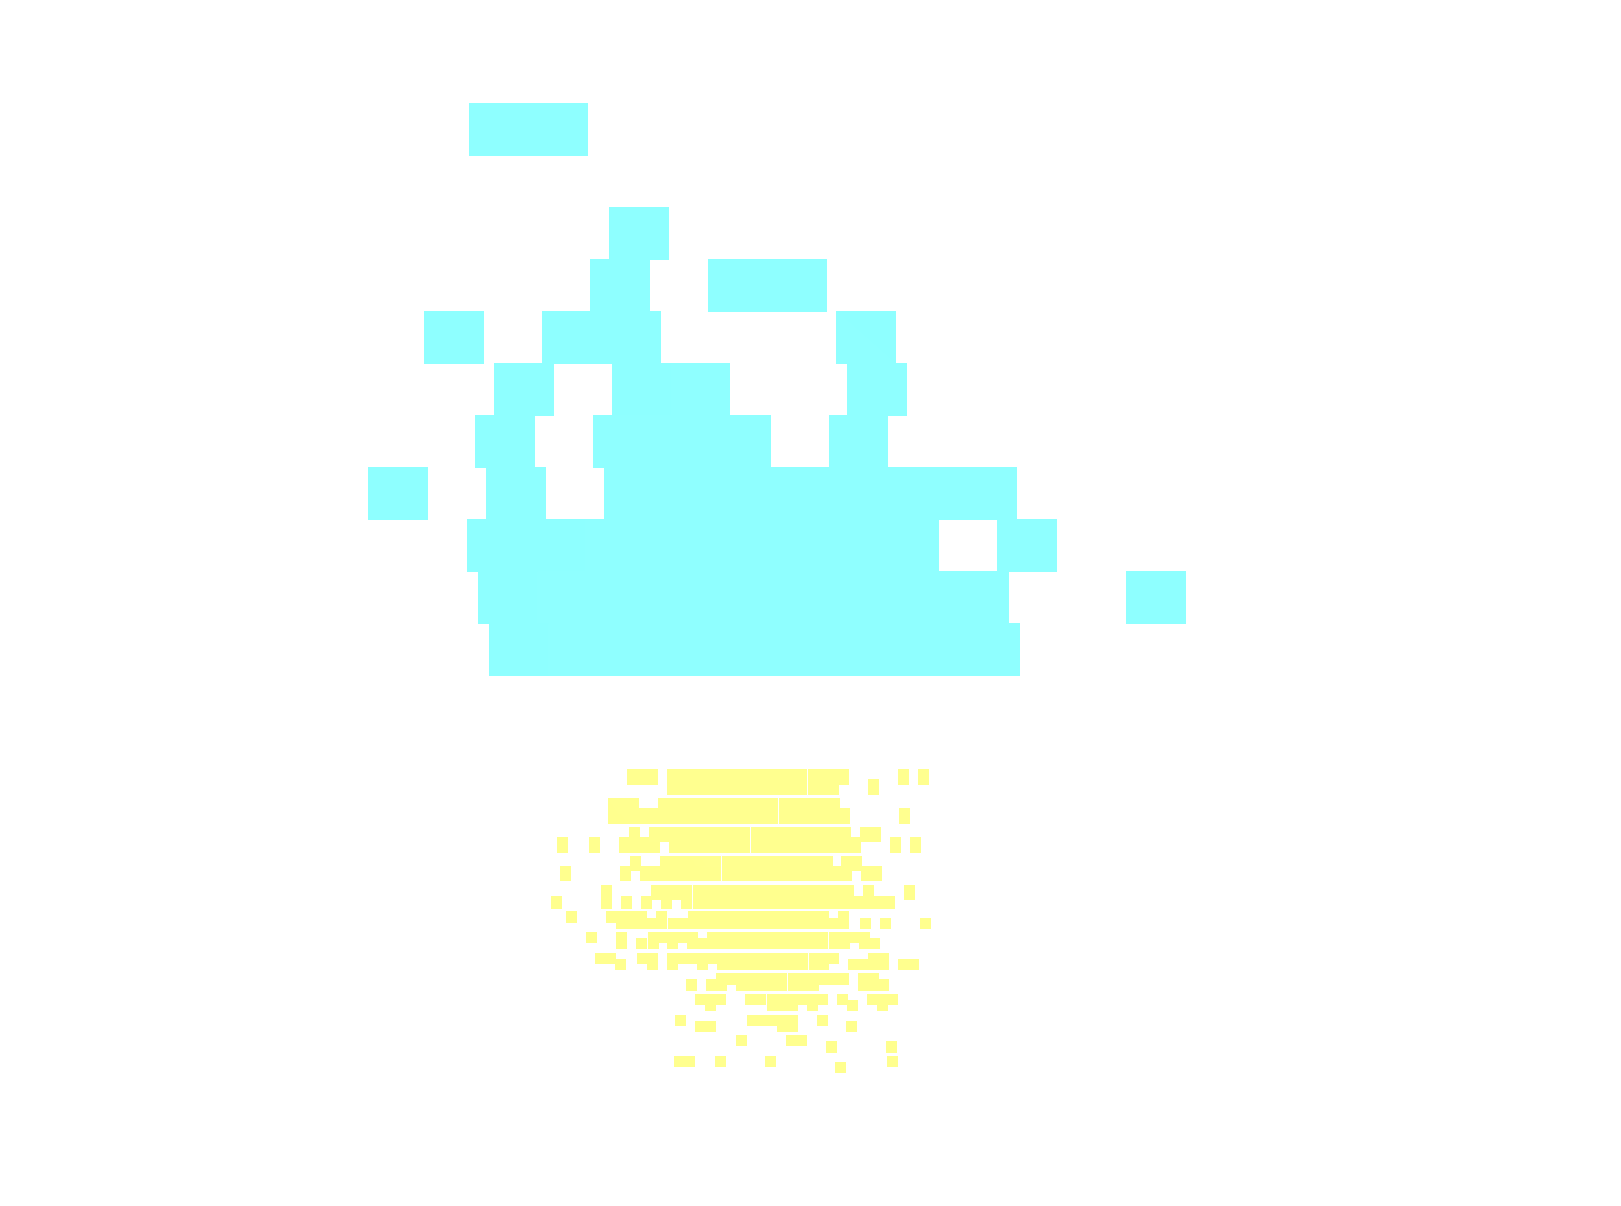
\includegraphics[width=0.5\textwidth]{photon/hcalfrag}}%
\caption{An event display of a typical 500\,GeV photon, reconstructed into a main photon in the \ECAL (yellow) and a neutral hadron fragment in the \HCAL (blue).}
\label{fig:photonEvtDspHCalFrag}
\end{figure}

With \Figure{fig:photonEvtDspHCalFrag} as an example, high energy fragments in the \HCAL is spatially close to the main photon. A fitted cone from the main photon covers most of the fragment if extended to the \HCAL. These features allow a set of cuts developed to merge high energy fragments, listed in \Table{tab:photonHighEnergyFragCuts}

This algorithm would collect the photons and neutral hadrons in the \HCAL as inputs. It occurs after the first pass of topological association in the reconstruction, which connects tracks to clusters in the \ECAL and the \HCAL. The algorithm would iterate over all pairs of reconstructed photons and neutral hadrons in the \HCAL. For each pair, a set of variables are calculated and compared to a set of cuts (\Table{tab:photonHighEnergyFragCuts}). Photon-fragment pairs passing the cuts will be merged.

\begin{table}[htbp]
\centering

\smallskip
\small
\begin{tabular}{l r }
\hline
High energy fragment recovery&  Cuts\\
\hline
\multicolumn{1}{L{0.3\textwidth}}{distance comparison} & \multicolumn{1}{R{0.3\textwidth}}{$d^l_c \leqslant 173\ \text{mm}$, $d^l_{cone} \leqslant 100\ \text{mm}$, $d_{cone} \leqslant 100\ \text{mm}$} \\
\multicolumn{1}{L{0.3\textwidth}}{shower width comparison} & \multicolumn{1}{R{0.3\textwidth}}{$  0.3 \leqslant \frac{w^l_f}{w^l_m} \leqslant 5$} \\
\multicolumn{1}{L{0.3\textwidth}}{projection comparison} & \multicolumn{1}{R{0.3\textwidth}}{$ r_f \leqslant 45\ \text{mm}$} \\
\multicolumn{1}{L{0.3\textwidth}}{energy comparison} & \multicolumn{1}{R{0.3\textwidth}}{$ \frac{E_f}{E_m} \leqslant 0.1$} \\
\multicolumn{1}{L{0.3\textwidth}}{cone comparison} & \multicolumn{1}{R{0.3\textwidth}}{$ \%{N_{calo,cone}} \geqslant 0.5$} \\
\hline

\hline
\end{tabular}

\caption[]%
{The cuts for merging high energy photon fragment in the \HCAL to the main photon in the \ECAL. $d^l_c$ is the distance between centroids of the last outer layer of the main photon and the first inner layer of the fragment. $d^l_{cone}$ is the distance between fitted cones using the last outer layer of the main photon and the first inner layer of the fragment. $d_{cone}$ is the distance between fitted cones using the main photon and the fragment. $w^l_m$ and $w^l_f$ are the r.m.s. width of the last outer layer of the main photon and the first inner layer of the fragment. $r_f$ is the r.m.s. mean energy weighted distance of a calorimeter hit in the fragment to the direction of the main photon. $E_m$ and $E_f$ are the main photon energy and the fragment energy. $\%{N_{calo,cone}}$ is the fraction of the calorimeter hits in the fragment in the extended fitted cone of the main photon.}
\label{tab:photonHighEnergyFragCuts}
\end{table}

Fragment in the \HCAL should be spatially close to the main photon, measured by three metrics. $d^l_c$ is the distance between centroids of the last outer layer of the main photon and the first inner layer of the fragment. $d^l_{cone}$ is the distance between fitted cones using the last outer layer of the main photon and the first inner layer of the fragment. $d_{cone}$ is the distance between fitted cones using the main photon and the fragment.

The direction of the fragment should be similar to that of the main photon. $r_f$, the r.m.s. mean energy weighted distance of a calorimeter hit in the fragment to the direction of the main photon, has to be small for merging.

Another feature of the fragment and the main photon is that the shower width should be similar. $w^l_m$ and $w^l_f$ are the r.m.s. width of the last outer layer of the main photon and the first inner layer of the fragment. The ratio $\frac{w^l_f}{w^l_m}$ needs to be in the range of 0.3 to 5. The generous upper bound is due to the \HCAL is coarser than the \ECAL.

When a fitted cone from the main photon is extended to the \HCAL, the cone should contain a significant amount of the fragment. $\%{N_{calo,cone}}$, the fraction of the calorimeter hits in the fragment in the extended fitted cone of the main photon, has to be no less than 0.5 for the merging.

The last criteria is the fragment should has low energy relative to the main photon. $E_m$ and $E_f$ are the main photon energy and the fragment energy. The ratio, $\frac{E_f}{E_m}$, has to be less than 0.1 for the merging.

If multiple photon-fragment pairs pass the cuts with the same fragment, the pair with highest $\%{N_{calo,cone}}$ will be merged.


\section{Photon splitting algorithm}
\label{sec:photonSplitting}

Algorithms described above deal with forming photons from calorimeter hits in the \ECAL, merging photon fragments in the \ECAL and the \HCAL. Another aspect in photon reconstruction is splitting accidentally merged photons. During the particle reconstruction, it is possible that photons are accidentally merged if they are spatially close. Hence another algorithm at the end of the particle reconstruction addresses this issue and tries to split merged photons.

Merged photon is typically energetic. The merged photon should be consistent with topologies of a spatially closed photon pair. Extra care should be taken if the photon is close to a charged \PFO. Many \pandora algorithms deal with track clusters association and there is a greater confidence in clusters associated with tracks. These features form logics behind the algorithm.

\begin{table}[htbp]
\centering

\smallskip
\small
\begin{tabular}{l r }
\hline
Photon splitting&  Cuts\\
\hline
\multicolumn{1}{L{0.3\textwidth}}{Cuts} & \multicolumn{1}{R{0.3\textwidth}}{$E > E_{c1}$, $E_{p2} > E_{c2}$, $N_{p} < 5$} \\
\hline
$E_{c1}$ and $E_{c2}$ values &  \\
\hline
\multicolumn{1}{L{0.3\textwidth}}{0 nearby charged \PFO} & \multicolumn{1}{R{0.3\textwidth}}{$E_{c1} = 10$, $E_{c2} = 1$} \\
\multicolumn{1}{L{0.3\textwidth}}{1 nearby charged \PFO} & \multicolumn{1}{R{0.3\textwidth}}{$E_{c1} = 10$, $E_{c2} = 5$} \\
\multicolumn{1}{L{0.3\textwidth}}{> 1 nearby charged \PFO} & \multicolumn{1}{R{0.3\textwidth}}{$E_{c1} = 20$, $E_{c2} = 10$} \\
\hline

\hline
\end{tabular}

\caption[]%
{The cuts for splitting photons, and the values for energy cut-off points. $E$ is the photon energy. $E_{p2}$ is  energy if the second largest peak from the two dimensional peak finding. $N_{p}$ is the number of peaks identified by the peak finding. $E_{c1}$ and $E_{c2}$ are the energy cut-off values, determined by the number of nearby charged \PFO{s}.}
\label{tab:photonPhotonSplitting}
\end{table}

The \Table{tab:photonPhotonSplitting} shows values for the splitting a photon. $E$ is the photon energy. $E_{p2}$ is  energy if the second largest peak from the two dimensional peak finding. $N_{p}$ is the number of peaks identified by the peak finding. $E_{c1}$ and $E_{c2}$ are the energy cut-off values, determined by the number of nearby charged \PFO{s}. When a energetic photon is identified, and a energetic second peak can be found by the peak finding, the photon is likely from a photon pair. $N_{p}$ cut is because a reconstructed photon is unlikely from more than four photons. The values of $E_{c1}$ and $E_{c2}$ allow more conservative approach when a photon is close to charged \PFO{s}. 



\section{Figures of merit}
\begin{figure}[tbph]
\centering
    \begin{subfigure}[b]{0.45\textwidth}
        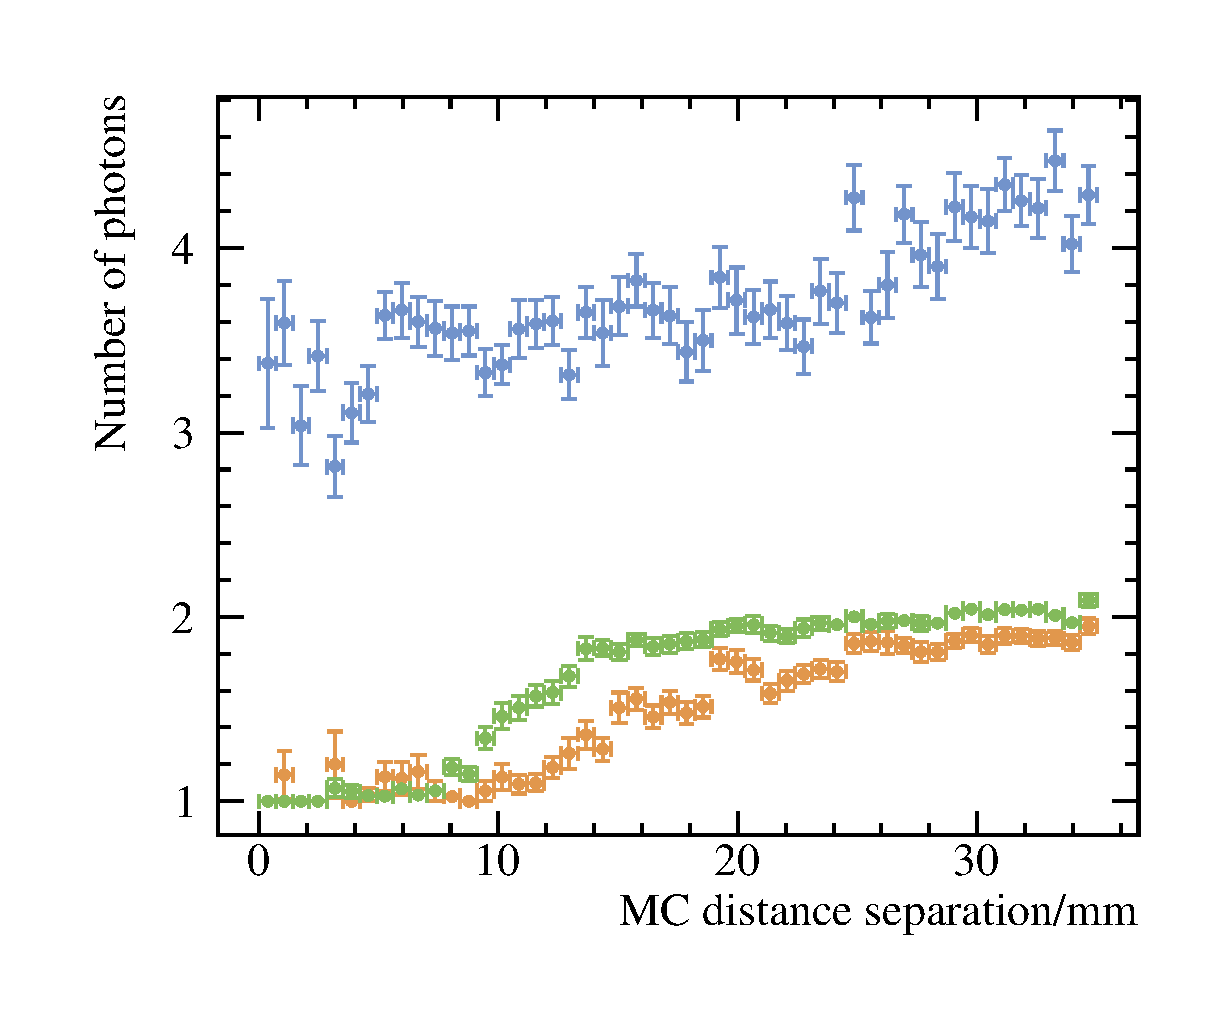
\includegraphics[width=\textwidth]{photon/n_p}
        \caption{}
        \label{fig:photonNumberOfPhoton}
    \end{subfigure}
    \begin{subfigure}[b]{0.45\textwidth}
        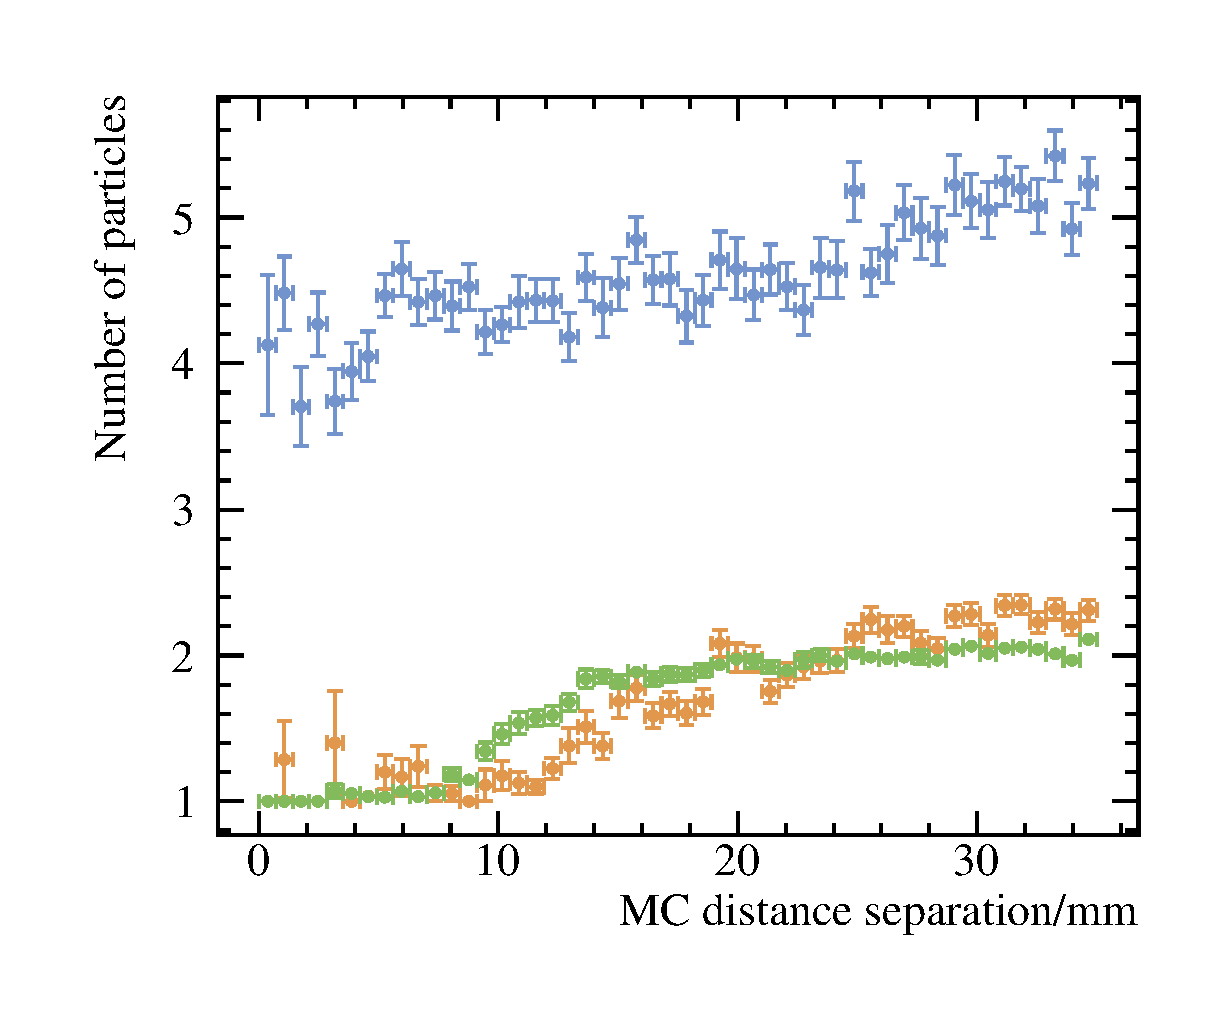
\includegraphics[width=\textwidth]{photon/n_all}
        \caption{}
        \label{fig:photonNumberOfParticle}
    \end{subfigure}

\caption[]
{\Figure{fig:photonNumberOfPhoton} shows the number of reconstructed photons as a function of their true distance separation for a two photons per event sample. \Figure{fig:photonNumberOfParticle} shows the number of reconstructed particle as a function of their true distance separation for a two photons per event sample. The top blue line is reconstructed with PandoraSettingsDefault.xml with iLCSoft v01-17-07. The bottom orange line is reconstructed with PandoraSettingsDefault.xml plus two fragment merging algorithm (RecoPhotonFragmentMergingAlgorithm and PhotonFragmentMergingAlgorithm). The middle green line is is reconstructed with PandoraSettingsDefault.xml plus all algorithms described above.
}
\label{fig:photonNPhoton}
\end{figure}





%The number of nearby charged \PFO{s} is defined by the number of charged \PFO{s}

\begin{comment}
Another type of photon fragment is caused when a highly energetic photon, typically more than 50GeV, goes through the ECal and deposits energy in the hadronic calorimeter (HCal), illustrated in \Fig{fig:evtDspHCalFrag}. Since the photon identification in PandoraPFA implicitly assumes that all photons are contained in the ECal, the energy deposited in the HCal either becomes neutral hadron fragments or part of a hadronic shower if a hadronic shower of another particle is nearby.

Similar to the treatment of fragments in the ECal, we merge the fragments in the HCal by calculating various quantities and place selection cuts. The important quantities are the distance between centroid for main photon and fragments, the distance of closest approach of the directions of the flights for main photon and fragments, and the fraction of energy in a fitted cone in HCal by extending the fitted cone from main photon in the ECal, where for main photon-fragment pairs, the distance metrics are small and the fraction of the energy in a fitted cone in HCal are large.

We implemented the algorithm in PandoraPFA (HighEnergyPhotonRecovery), after the standalone photon reconstruction algorithm, which successfully remove most of photon fragments in the HCal for high energy photons, as shown in \Fig{fig:n_all}.
\end{comment}

%To merge photon fragments to the main photon, we carefully compare distributions of various quantities for main photon-fragment pairs and main photon-other particles pairs, and choose cuts that would merge fragments to main photons and not merge other particles to main photons. The most useful distances related parameters are the simple distance between centroids of the pair, and the mean intra-layer distance weighted over energy between the pair, where the main photon-fragment pairs should have a small distance metric and main photon-non-photon particles pairs would have larger ones. The other useful method is the energy deposition of the pair in a transverse plane perpendicular to the direction of the flight, where the main photon-fragment pairs produce a single peak in the two dimensional shower, and the main photon-non-photon particles pairs produce two peaks in the two dimensional shower.

%Based on this, two algorithms have been carefully implemented to merge fragments in electromagnetic calorimeter to the main photons. One algorithm (RecoPhotonMergingAlgorithm) is placed immediately after the standalone photon identification. The other one (PhotonMergingAlgorithm) is placed at the end of the reconstruction chains in PandoraPFA. The two algorithms provide an excellent reduction in the number of fragments created, as shown in \Fig{fig:nPhoton}.




%Discriminating variables of each candidate are calculated. The variables are used for trainning the classifier and for the classification.



The default histogram size is 41 by 41 bins.



The input of the two dimensional peak finding algorithm is a two dimensional histogram.













\begin{comment}
When a high-energy electron or photon is incident on a thick absorber, it initiates
an electromagnetic cascade as pair production and bremsstrahlung generate more
electrons and photons with lower energy.

The longitudinal development is governed by
the high-energy part of the cascade, and therefore scales as the radiation length in the
material. Electron energies eventually fall below the critical energy, and then dissipate
their energy by ionization and excitation rather than by the generation of more shower
particles.

The distributions
are characterized by a narrow core, and broaden as the shower develops. They are often
represented as the sum of two Gaussians,
\end{comment}
%The core part of the standalone photon reconstruction algorithm is to identify peaks in a 2D plane, the energy deposition of a transverse 2D plane perpendicular to the direction of the flight. Each identified peak will form a cluster. The cluster will be identified as a photon if it passes the photon likelihood test. The key to improve photon separation resolution is to improve the 2D peak finding algorithm. We have implemented a new peak finding algorithm, which finds all possible local maxima. Other cells in the 2D plane are associated to each peak by minimising the metric $d/\sqrt(E)$, where $d$ is the distance in 2D plane from the cell to the peak, and $E$ is the energy or height of that particular peak. \Fig{fig:peakFinding} shows two energetic photons just resolved with the new 2D peak finding algorithm.


%The standard reconstruction reconstructs muons before this step. Hence ideally the hits in the \ECAL belong to photons or charged hadrons.


  \chapter{Tau Lepton Decay Modes Classification}
\label{chap:Tau}

\chapterquote{Give a man a fish and you feed him for a day; teach a man to fish and you feed him for a lifetime.}%
{}%: Blackwood's Magazine May 1830

The tau lepton has been studied extensively in the past at the Large Electron Positron Collider (LEP)\cite{Schael:2005am}. The tau lepton spin state, which can be derived from kinematic properties of its decay products, can be used to measure the CP (the product of charge conjugation and parity symmetries) of the Higgs, via \HiggsToTauTau channel\cite{Berge:2015nua}.  The polarisation correlation of the tau pairs can be used to infer the spin of the parent boson, differentiating \HiggsToTauTau from \ZToTauTau.

\begin{comment}
\FIGURE{fig:tauTheorySpin} shows an example of  difference in distributions for the two channels.
\begin{figure}[!htbp]
\centering
% \begin{center}/\end{center} takes some additional vertical space
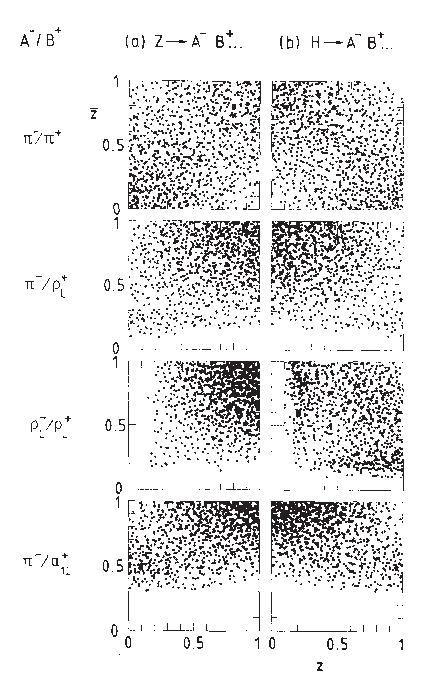
\includegraphics[width=.45\textwidth]{tau/theory}
\caption[An example of  difference in distributions for \HiggsToTauTau and \ZToTauTau.]
{
The two-dimensional distribution of (a) \HepProcess{\PZ \to \APtauon \Ptauon \to A^- B^+ \Pnut \APnut } (b) \HepProcess{\PHiggs \to \APtauon \Ptauon \to A^- B^+ \Pnut \APnut } events shown as functions of the energy fractions of $z = E_{A} / E_{\Ptauon}$ and $\overline{z} =  E_{B} / E_{\APtauon}$. In descending order the four sets of plots are for the (\APtauon, \Ptauon) pair decaying into (\Ppiminus, \Ppiplus), (\Ppiminus, $\rho_L^+$), ($\rho_L^-$, $\rho_L^+$) and finally (\Ppiminus, $a_{1L}^+$), each together with a \Pnut \APnut neutrino-pair. Plot is taken from \cite{Bullock:1991my}.
}
\label{fig:tauTheorySpin}
\end{figure}
\end{comment}

The ability to identify tau decay mode can also a benchmark for detector performance. Since tau lepton has a very short lifetime of 290\,fs \cite{Abreu:1991jn,Agashe:2014kda}, only its decay products can be detected with the tracking detectors and calorimeters. Therefore the performance of the calorimetric and track systems determines the ability to reconstruct the tau lepton decay products and identify different tau decay modes.


The main challenge in the tau lepton decay modes  classification is to reconstruct and separate spatially close photons. Many final states of the tau decay involves \Ppizero, where \HepProcess{\Ppizero \to \Pphoton \Pphoton}. For some final states, the one difference in the topology is the number of photons. At high centre-of-mass energy, the decay product of the tau decay are often boosted.  To reconstruct two photons from \Ppizero decay  separate entities requires good pattern recognition algorithms for photons and a \ECAL spatial resolution. Hence the photon reconstruction dedicated in \Chapter{chap:Photon} is used in this study to identify photons.

This chapter is organised as follows. Firstly, the analysis chain to identify tau decay modes will be described. The performance of the tau decay mode classification will be given, followed by the \ECAL optimisation study using the decay mode classification as a benchmark. Lastly, the  tau decay mode classification is further used in a proof-of-principle analysis to demonstrate the ability to identify \PHiggs from \PZ using  tau pair decay channel.

%
%The impact of the \ECAL transverse spatial resolution on the tau decay classification is demonstrated as well.



\section{Overview of the analysis}

The analysis starts with defining the samples for study in \Section{sec:tauDecayModes}. The seven major tau lepton decay modes are chosen for the classification. The simulation and reconstruction of these tau lepton decay are described in \Section{sec:tauSim}.  Pre-selection of the events, discussed in \Section{sec:tauPreSel}, are such that the reconstruction and detector effect, which do not vary with the \ECAL cell sizes, are not included in this analysis. After defining discriminative variables in \Section{sec:tauVar}, the classification is performed with a multivariate classifier. Since one decay mode needs to be classified into one of the seven decay modes, a multiclass classicisation is used to allow simultaneous classification between  multiple final states, which is presented in \Section{sec:tauMVA}.

The classification of the tau lepton decay modes are then  repeated for different energies of tau lepton decay to access the impact of the energy on classification. The classification is also used to study the effect of the \ECAL cell size on the classification performance. The impact of the tau energy and the \ECAL cell size on the classification performance is discussed in \Section{sec:tauECAL}. Lastly, the classification is utilised to demonstrate the ability to separate \PHiggs from \PZ using  tau pair decay channel in a proof-of-principle analysis, described in the \Section{sec:tauHZ}.

% The difference in the spin of the boson reflects in the different spin correlation of the tau pair. By extracting the spin correlation, parent bosons can be separated.
%This classification is repeated for different energies of tau lepton decay to access the impact of energy on classification. The impact of the \ECAL design is studied afterwards, where the \ECAL square cell size is varied. An overall tau hadronic decay classification efficiency is constructed to allow direct and easy comparison between different detector design and different energies of the tau decay.

% The study of the tau final state classification in the context for the  \ECAL optimisation allows the analysis to discard reconstruction and detector issue that do not vary with the \ECAL design. For example, the early photon conversion that happens in the tracking detector would complicate the event topology. But since it is affected by the tracker design, it can be ignored in this analysis. \SECTION{sec:tauSim}  and \Section{sec:tauPreSel} discuss the pre-selection cuts to choose the signal samples and events for this analysis.

%The classification is performed with a multivariate classifier. Discriminating variables are calculated before feeding into the classifier.  A multiclass classicisation is used to allow simultaneous classification between  multiple final states, described in \Section{}.


%A proof-of-principle analysis to demonstrate the ability to identify \PHiggs from \PZ using  tau pair decay channel is presented in the \Section{}. The difference in the spin of the boson reflects in the different spin correlation of the tau pair. By extracting the spin correlation, parent bosons can be separated.

%The follow sections on the analysis use the a 50\,GeV tau lepton decaying sample, reconstructed with nominal the \ILD detector model.

\section{Samples for the analysis}
\label{sec:tauDecayModes}

%\section{Select single tau decay}
Simplest tau lepton decay channel in a \ee collider is chosen: \eeToTauTau, with centre-of-mass energy of 100\,GeV.  An example of the simulated \eeToTauTau event is shown in \Figure{fig:tauEvtDsp}. The \eeToTauTau channel contains two tau leptons travelling in opposite directions. Since the tau decay final state separation is applicable to a single tau lepton, particles in one event are divided into two collections. Each collection corresponds  to the decay products of one tau lepton.

The principle thrust axis vector is used to separation particles into two collections. Two collections are obtained based on the sign of the scalar product between the principle thrust axis vector  and the particle momentum vector. The classical event shape thrust, $T$,  \cite{PhysRevLett.39.1587}, is defined as
\begin{equation}
T = \max_{\hat{t}}\!\frac{\sum_{i}\absOf{\hat{t}\!\cdot\!\vec{p_{i}}}}{\sum_{i}\absOf{\vec{p_{i}}}}
\end{equation}
where $\vec{p_{i}}$ is the momentum vector of the particle $i$;   $\hat{t}$, is a unit principle thrust axis vector; and the summation is over all particles in an event. Thrust axis is useful to separate each jet in a back-to-back two-jet event.
%Thrust value, $T$, is 1 for a perfect pencillike back-to-back two-jet event, and 0.5 for a perfect spherical event. The thrust value is useful in picking out back-to-back two-jet event.


\begin{figure}[tbph]
\centering
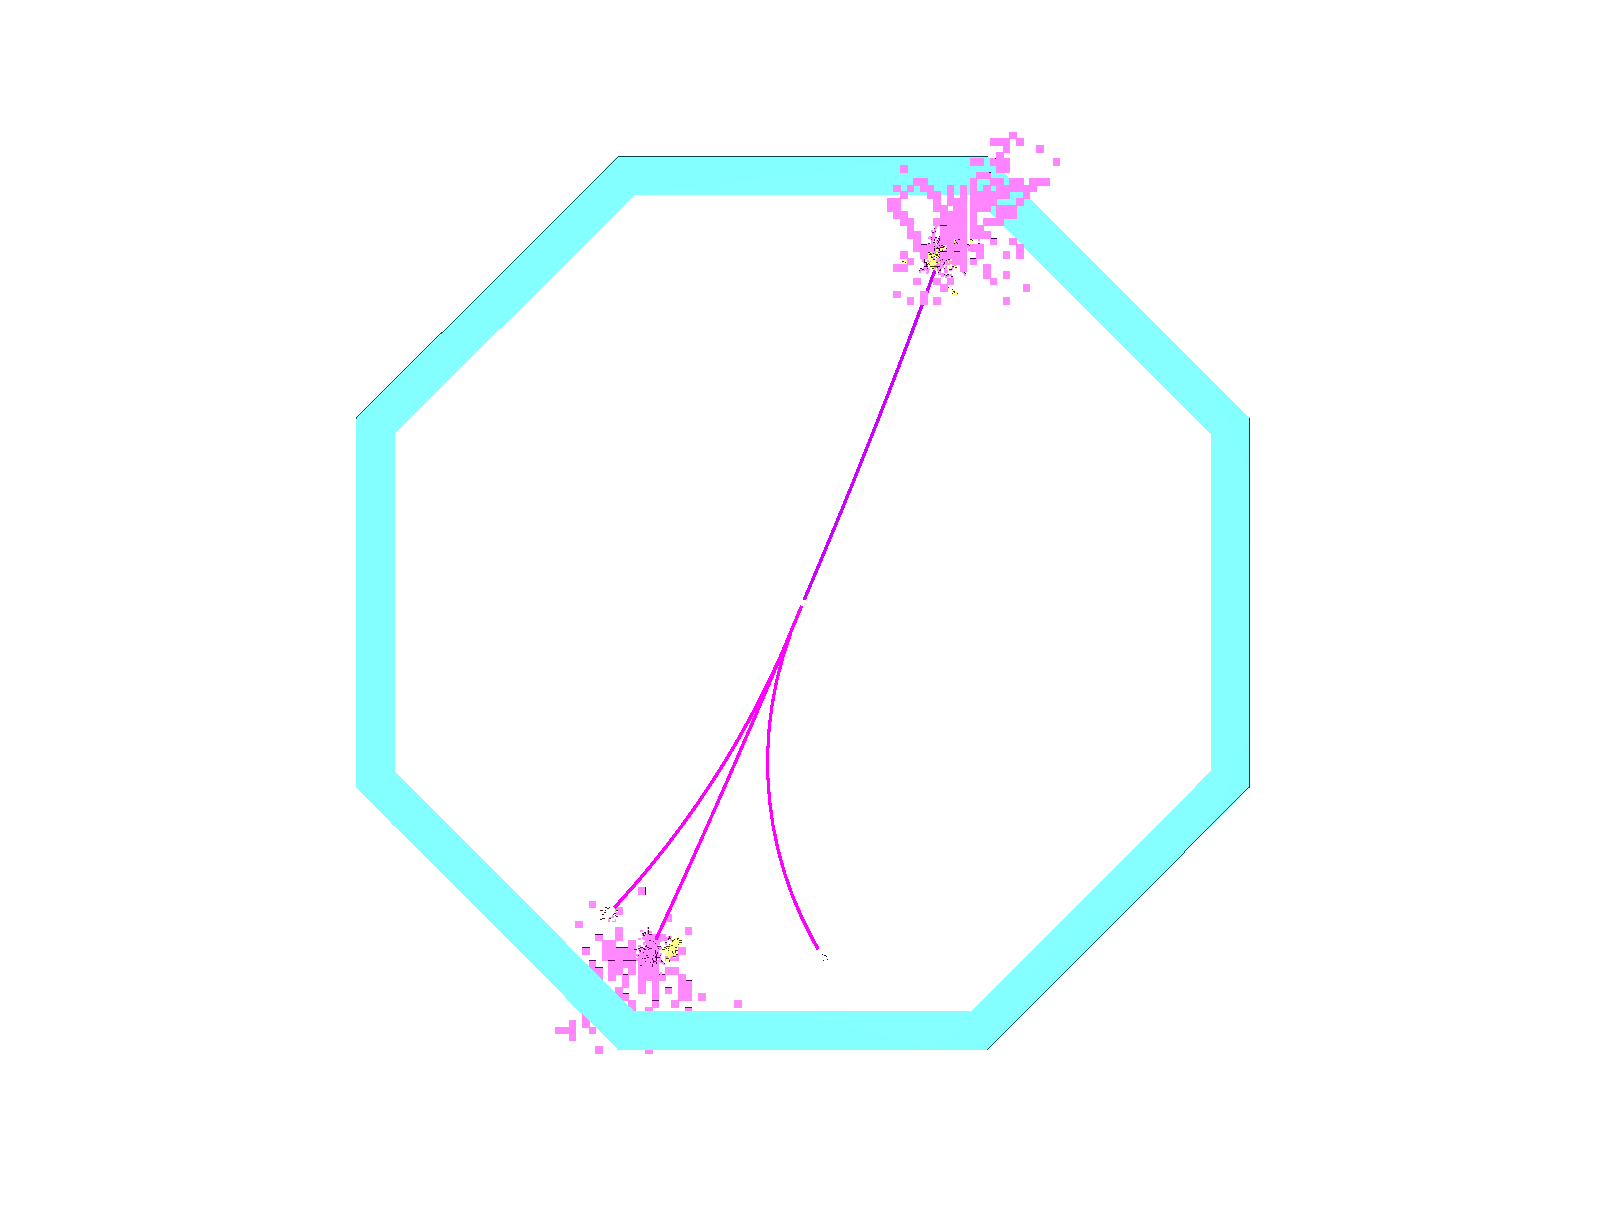
\includegraphics[width=0.65\textwidth]{tau/tau_evt_dsp2}
\caption{ An example event display of a simulated \eeToTauTau event using a \ILD detector model. The top half of the event is a tau lepton decaying into \decayRhoFinalStateShort final state and the bottom half of the event is a tau lepton decaying into  \decayThreePionPhotonShort final state. The purple lines are the tracks left by \Ppipm in the tracking detector. The purple clusters are the energy deposition by \Ppipm and the yellow clusters are the energy deposition by photon from \HepProcess{\Ppizero \to \Pphoton \Pphoton}. The blue region is the transverse cross section of the \ECAL barrel along the beam line direction.}
\label{fig:tauEvtDsp}
\end{figure}

\subsection{Tau lepton decay modes}

Tau lepton decays into a numerous number of final states. To study the predominant effect of the tau lepton decays, decay modes with branching ratio above 2\% are studied. This results in seven tau lepton decay modes. Their branching ratios, along with decay modes and final states are  shown in \Table{tab:TauDecayMode}. The seven tau lepton decay modes, which cover 92.58\,\% of all tau decay, are chosen to study in this analysis

% The most difficult final states to separate are \decayRhoFinalStateShort and \decayAiPhotonFinalStateShort, where photons from boosted \Ppizero are very challenging to reconstruct correctly.

\begin{table}[htbp]\centering
\smallskip
\begin{tabular}{l l r}
\hline
\hline
Decay modes & Detectable final states & Branching ratio\\
\hline
\decayElectron   &  \decayElectronShort  & $17.83\%_{\pm0.04\%}$   \\
\decayMuon &	\decayMuonShort & $17.41\%_{\pm0.04}$  \\
\decayPion  &   \decayPionShort	& $10.83\%_{\pm0.06}$   \\
\decayRho   & \decayRhoFinalStateShort& $25.52\%_{\pm0.09\%}$ \\
\decayAi   & \decayAiPhotonFinalStateShort	& $9.30\%_{\pm0.11\%}$    \\
\decayAi  &	\decayAiPionFinalStateShort    & $8.99\%_{\pm0.06\%}$  \\
\decayThreePionPhoton  &	\decayThreePionPhotonShort    & $2.70\%_{\pm0.08\%}$  \\
\hline
\hline
\end{tabular}
\caption[Decay modes, detectable final state particles and branching ratios of the seven major \Pgtm decays.]
{Decay modes, detectable final state particles and branching ratios of the seven major \Pgtm decays, taken from \cite{Agashe:2014kda}. \Pgtp decays similarly to \Pgtm.}
\label{tab:TauDecayMode}
\end{table}

\section{Simulation and reconstruction}
\label{sec:tauSim}

Two million \eeToTauTau events are simulated and reconstructed. The \ILD detector model was used. As the study is aimed for optimisation study of the \ECAL cell sizes, the beam specific effects does not vary with the \ECAL cell sizes are not simulated.  These effects include the initial state radiation (ISR) and the beam induced background.


The software used for simulation and reconstruction is described in \Chapter{chap:Reconstruction}. Events are reconstructed with  \ilcsoft version v01-17-07 \cite{Gaede:82475} and \pandora version 3 \cite{Marshall:2015rfa}, where the photon reconstruction is discussed in \Chapter{chap:Photon}.


\section{Event pre-selection}
\label{sec:tauPreSel}

Since the analysis is aimed for the optimisation of the \ECAL cell sizes, pre-selection cuts that are not affected by the \ECAL cell sizes are used. These cuts also allow the analysis to focus on the events with clear topologies. The pre-selection cuts are listed in \Table{tab:tauPreSel}. The fraction of events passing each pre-selection cut for individual decay mode are listed in \Table{tab:tauPreSelEff}.

One of the pre-selection cuts is to demand that the event does not have photons converted to electron pairs in the tracking detector. These discarded events would have few photons and more electrons in the final states, which changes the topologies of the final states. Shown in \Table{tab:tauPreSelEff}, only decay modes with photons in the final states are affected by this cut, as expected.


Another pre-selection cut is the total energy of the non-neutrinos tau decay products, $E_{vis,MC}$, > 5\,GeV, based on the truth information. If most energy of the tau lepton is carried by the neutrinos, it is difficult to identify the low-energy non-neutrino tau decay products. Hence these events with low energy of the non-neutrinos tau decay products are not used in the analysis. Decay modes with only one non-neutrino particle in the final states are mostly affected by this cut, indicated in \Table{tab:tauPreSelEff}.

The last pre-selection cut is to avoid events with energy deposition in the gap region between barrel and the end cap part of the calorimeter. As the reconstruction   does not attempt to recover reconstruction in the gap region, threw is a significant drop in the particle reconstruction efficiency. The cut demands the absolute value of the polar angle of tau lepton,  $\absOf{\theta_{Z,MC}}$, based on the truth information, is between 0.3 and 0.6\,rad to be contained in the end cap region, or is between 0.8 and 1.57 to be contained in the barrel region. All decay modes are affected almost equally by this cut, suggested by the numbers in \Table{tab:tauPreSelEff}.


\begin{table}[htbp]\centering
\smallskip
\begin{tabular}{l r}
\hline
\hline
Cuts & Values\\
\hline
\multicolumn{1}{L{0.4\textwidth}}{Photon conversion in the tracking detector}& No \\
\multicolumn{1}{L{0.4\textwidth}}{Total energy of non-neutrino decay products} & $E_{vis,MC} > 5\,GeV$ \\
Polar angle acceptance & \multicolumn{1}{R{0.5\textwidth}}{$0.6 > \absOf{\theta_{Z,MC}} > 0.3$ or $1.57 > \absOf{\theta_{Z,MC}} > 0.8$} \\
\hline
\hline
\end{tabular}
\caption[Pre-selection cuts for tau lepton decay final state classification.]
{Pre-selection cuts for tau lepton decay modes classification.}
\label{tab:tauPreSel}
\end{table}


\begin{table}[htbp]\centering
\smallskip
\begin{tabular}{ l r r r}
\hline
\hline
 \multicolumn{1}{R{0.2\textwidth}}{Detectable final state}   & \multicolumn{1}{R{0.25\textwidth}}{No photon conversion in the tracking detector} & \multicolumn{1}{R{0.25\textwidth}}{Total energy of non-neutrino decay products acceptance} &\multicolumn{1}{R{0.25\textwidth}}{Polar angle acceptance} \\
\hline
\decayElectronShort& 100.0\% & 84.7\%& 66.2\%\\
\decayMuonShort &100.0\%& 85.2\%&66.7\%\\
\decayPionShort &100.0\%& 88.3\%&60.9\%\\
\decayRhoFinalStateShort &77.1\%&76.9\%&61.9\%\\
\decayAiPhotonFinalStateShort &61.3\%&61.2\%&50.5\%\\
\decayAiPionFinalStateShort &100.0\%&100.0\%&78.0\%\\
\decayThreePionPhotonShort &77.0\%&77.0\%&61.8\%\\
\hline
\hline
\end{tabular}
\caption
{The fraction of events passing each pre-selection cut for individual decay mode. Cuts are presented in a ``flow'' fashion, where each column contains all the cuts to its left.}
\label{tab:tauPreSelEff}
\end{table}

%The no photon early conversion cuts only effective against final states with \Ppizero, as \Ppizero decays to a photon pair. For final states with one \Ppizero, about 77\% events survived. For final states with two \Ppizero, about 61\% events survived, which is roughly $0.77^2$. For the visible angle acceptance, final states with only one particle are affected the most, whilst final states with more than one particles typically have more visible energies. The polar angle acceptance efficiencies depend on the final states, as light final states are boosted and more likely in the forward region.



%An low visible energy event is discarded if the total energy of the tau lepton visible decay products is below 5\,GeV. Requirement of the tau decay in the barrel or the end cap part of the calorimeter is defined as the polar angle of the tau is $ 17.2\degree < |\theta_{Z}| < 34.4\degree$ or $ 45.8\degree < |\theta_{Z}| < 90\degree$.





\section{Variables used in the MVA}
\label{sec:tauVar}


Having pre-selected events, discriminating variables are carefully developed for the multivariate analysis (MVA). The full list of the variables are shown in \Table{tab:tauVaraibles}. The distribution of the four most power variables are shown in \Figure{fig:tauVar}.

\subsection{\PFOs number variables}

The most crucial variables are the number of \PFOs of different particles. There are five \PFOs number variables used in MVA event selection: the number of charged particles (${N}_{\charge}$); the number of muons (${N}_{\Pmu}$); the number of electrons (${N}_{\Pe}$); the number of photons (${N}_{\Pgg}$); and the number of charged pions (${N}_{\Pgpm}$).

\FIGURE{fig:tauVarNCharge} shows the distributions of the number of charged particles for selected tau decay modes. Whilst over 98\% 1-prong final states have one track reconstructed, around 95\%  3-prong final states have three tracks reconstructed. The distributions of the number of photons are shown in \Figure{fig:tauVarNPhoton}. The overlap between the distribution for \decayPionShort and \decayRhoShort decay modes is about 10\% of the \decayPionShort events and 20\% of the \decayRhoShort events.

% and the overlap between \decayRhoShort and \decayAiPhotonShort is around 15\%. ${N}_{\Pgg}$ can also separate two 3-prong final states.
%${N}_{\Pmu}$, ${N}_{\Pe}$, ${N}_{\Pgpm}$ are useful to identify two leptonic final states, and further separate 3-prong final states from 1-prong final states.
%This is an excellent variable to separate 1-prong and 3-prong final states.  An orthogonal measurement is the number of reconstructed photons,  ${N}_{\Pgg}$, shown in \Figure{fig:tauVarNPhoton}.

\subsection{Invariant mass variables}

Five invariant mass variables participate the MVA event selection: the invariant mass of all visible decay products ($m_{vis}$); the invariant mass of all charged particles ($m_{\charge}$); the invariant mass of all neutral particles ($m_{\neutral}$); the invariant mass of all photons ($m_{\Pgg}$); and the invariant mass of all charged pions ($m_{\Pgpm}$). \FIGURE{fig:tauVarMVis} shows distribution of the invariant mass of all visible decay products for selected tau decay modes. Reasonable structures can be seen for \Prho and \Pai decay modes.

%Invariant masses of different particles are good at characterising different final states. \FIGURE{fig:tauVarMVis} shows the invariant mass of the system. Clear reasonable peaks can be seen for \Prho and \Pai. The mass peak of  \decayAiPionFinalStateShort are much higher. $m_{\charge}$ and $m_{\neutral}$ are invariant masses of charged and neutral particles respectively. They separate final states with neutral particles from those without neutral particles. Similarly, $m_{\Pgg}$ and $m_{\Pgpm}$ identify final states with photons and with \Pgpm respectively.

\subsection{Energy variables}

Energy information further separate different final states. Six energy variables are used in the MVA event selection: the normalised total energy of all visible decay products ($\tilde{E}_{vis}$); the normalised total energy of the charged particles ($\tilde{E}_{\charge}$); the normalised total energy of the muons ($\tilde{E}_{\Pmu}$); the normalised total energy of the electrons ($\tilde{E}_{\Pe}$); the normalised total energy of the photons ($\tilde{E}_{\Pgg}$); and the normalised total energy of the charged pions ($\tilde{E}_{\Pgpm}$). All variables are normalised with respect to the energy of the associated tau lepton.

\subsection{Calorimetric information variable}


Two calorimetric information variable are used in the MVA event selection: the fraction of the  deposited in the \ECAL over the total energy in the calorimeters for all charge particles ($\% E_{\charge}$) and the fraction of the  deposited in the \ECAL over the total energy in the calorimeters for all particles ($\% E$). Calorimetric information is used to identify electron and muon. An electron deposits most energy in the \ECAL and a muon deposits 5 to 20\% energy in the \ECAL. The difference between two variables is that the contribution from photons, which also deposit most energy in the \ECAL like electrons, do not participate in the calculation of $\% E_{\charge}$.



\subsection{\texorpdfstring{\decayRhoShort and \decayRhoShort} \, resonances reconstruction variables}
\label{sec:tauResonance}
\decayRhoShort and \decayAiPhotonShort are identified further using their resonance structure. For example, \decayRhoShort decay mode contains a \Pgpm and a \Ppizero decaying into two photons. By selecting \Pgpm and photons consistent with \Prho decay pattern, \decayRhoShort decay mode could be identified. The  \decayRhoShort decay mode hypothesis test performed by minimising a  $\chi^{2}$ function:
\begin{equation}
\chi^{2} = {\left(\frac{m_{tot} -  m^{MC}_{\Prho}}{\sigma^{MC}_{\Prho}}\right)}^{2} + {\left(\frac{m_{\Pphoton \Pphoton} -  m^{MC}_{\Ppizero}}{\sigma^{MC}_{\Ppizero}}\right)}^{2} \,,
\end{equation}
where $m_{\Pphoton \Pphoton}$ is the invariant mass of two photons; $m_{tot}$ is the invariant mass of the  two photons and one \Pgpm; $m^{MC}_{\Prho}$ and $m^{MC}_{\Ppizero}$ are expected masses of \Prho and \Ppizero, respectively, taken from \cite{Agashe:2014kda}; and $\sigma^{MC}_{\Prho}$ and $m^{MC}_{\Ppizero}$ are the half width of the invariant mass distribution of reconstructed \Prho and \Ppizero, respectively , obtained using the truth information. All combinations of photons and \Pgpm are tested. Two variables obtained in this minimisation and used in the MVA event selection are the invariant mass of the two photons in the fit ($m_{\Pgpz}\parenths{\rho}$) and  the invariant mass of the  two photons and one \Pgpm ($m_\rho$).


Similarly, \decayAiPhotonShort decay mode can be identified using a extended minimisation $\chi^{2}$ with two extra photons:
\begin{equation}
\chi^{2} = {\left(\frac{m_{tot} -  m^{MC}_{\Pai}}{\sigma^{MC}_{\Pai}}\right)}^{2} + {\left(\frac{m_{\Pphoton1 \Pphoton2} -  m^{MC}_{\Ppizero}}{\sigma^{MC}_{\Ppizero}}\right)}^{2}  + {\left(\frac{m_{\Pphoton3 \Pphoton4} -  m^{MC}_{\Ppizero}}{\sigma^{MC}_{\Ppizero}}\right)}^{2} \,,
\end{equation}
where \Prho has been replace by \Pai and other variables are defined in the same way as in the previous $\chi^2$ function. Two photon pairs and one \Pgpm are needed for this minimisation. Both photon pairs are required to be consistent with \HepProcess{\Ppizero \to \Pphoton \Pphoton}. Three variables obtained in this minimisation and used in the MVA event selection are the invariant mass of the first two photons in the fit ($m_{\Pgpz}\parenths{\Pai}$); the invariant mass of the last two photons in the fit ($m^*_{\Pgpz}\parenths{\Pai}$); and the invariant mass of the four photons and one \Pgpm ($m_{\Pai}$). The first photon pair is defined to have a invariant mass closer to the invariant mass of the \Ppizero than the second photon pair.  \FIGURE{fig:tauVarMA1} shows the distributions of the invariant mass of the four photons and one \Pgpm under \decayAiPhotonShort hypothesis test for selected tau decay modes. Only the distribution for \decayAiPhotonShort decay mode has a resonance peak at \Pai mass.

%Comparing to simple invariant mass distribution in \Figure{fig:tauVarMVis}, \decayAiPhotonShort mass peak is enhanced.
%\decayAiPhotonShort reconstruction &  \multicolumn{1}{R{0.6\textwidth}}{  $m_{\Pgpz}\parenths{\Pai}$, $m^*_{\Pgpz}\parenths{\Pai}$, $m_{\Pai}$} \\

The $\chi^{2}$ functions for both hypothesis test are adapted for events where reconstruction fails to reconstruct enough photons. Relevant photon terms are dropped from the expression if there are fewer photons reconstructed  than required in the $\chi^{2}$ functions.

\subsection{Separate \decayElectronShort from \decayPionShort}

The Particle ID reported from \pandora is used extensively to reconstruct variables. \pandora uses a wide range of information to determine electron the ID. However, extra information is used in this analysis to help identifying electrons, which could be mistaken as \Pgpm by \pandora reconstruction.

An electron leaves a characteristic electromagnetic  (EM) shower in the \ECAL (see \Section{sec:photonEMshower}), whilst \Pgpm doesn't. Variables defining the  EM shower helps to identify \Pem, taken from photon reconstruction in \Section{sec:photonLikelihood}. Three variables are used in the MVA event selection: the start layer of the longitudinal shower ($t_0$); the fractional difference between observed and expected longitudinal shower profile describe the longitudinal EM shower ($\delta{l}$); and $\langle{w}\rangle$, a measure of the EM shower transverse width.

Another type of information to differentiate an EM shower from a \Pem and a early hadronic shower from a \Pgpm is the calorimeter hit information. Two variables used in the MVA event selection are: the average energy of a calorimeter hit ($\bar{E}_{hit}$) and the fraction of possible minimum ionising particles for all particles ($\%MIP$)

Last information used to separate \Pem from \Pgpm is the track-momentum-calorimeter-energy consistency check. The variable used in the MVA event selection is the calorimeter energy divided by the track momentum for all particles ($\Delta E/P$).

%This variable is found to help to differentiate \decayElectronShort from \decayPionShort final state.


%EM shower profile & $\delta{l}$, $t_0$, $\langle{w}\rangle$ \\
%Calorimeter hit info. & $\bar{E}_{hit}$, $\%MIP$ \\
%Track info. & $\Delta E/P$ \\




\begin{figure}[htbp]
\centering
% \begin{center}/\end{center} takes some additional vertical space
\begin{subfigure}[b]{0.45\textwidth}
 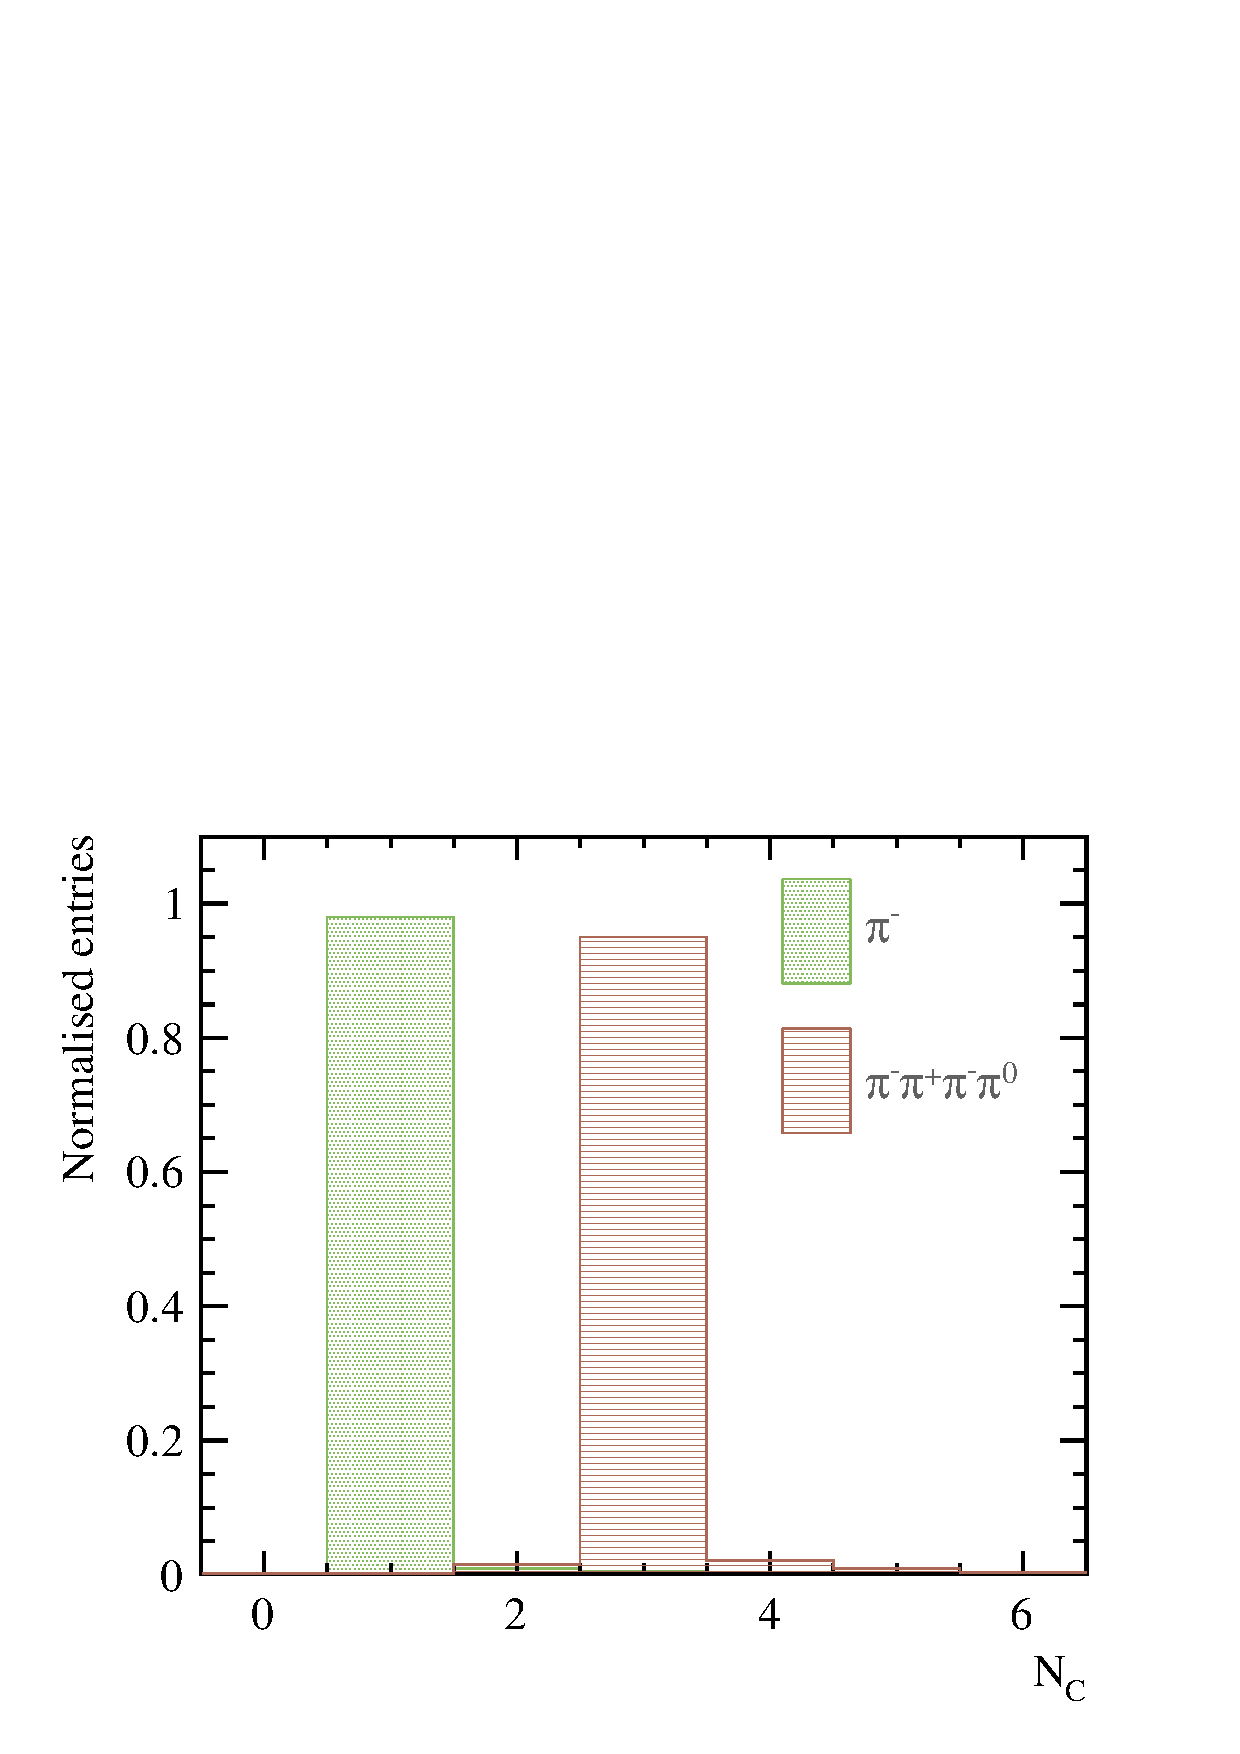
\includegraphics[width=\textwidth]{tau/var2/nCharge_100GeV_improved.pdf}
  \caption{}
  \label{fig:tauVarNCharge}
\end{subfigure}
\begin{subfigure}[b]{0.45\textwidth}
 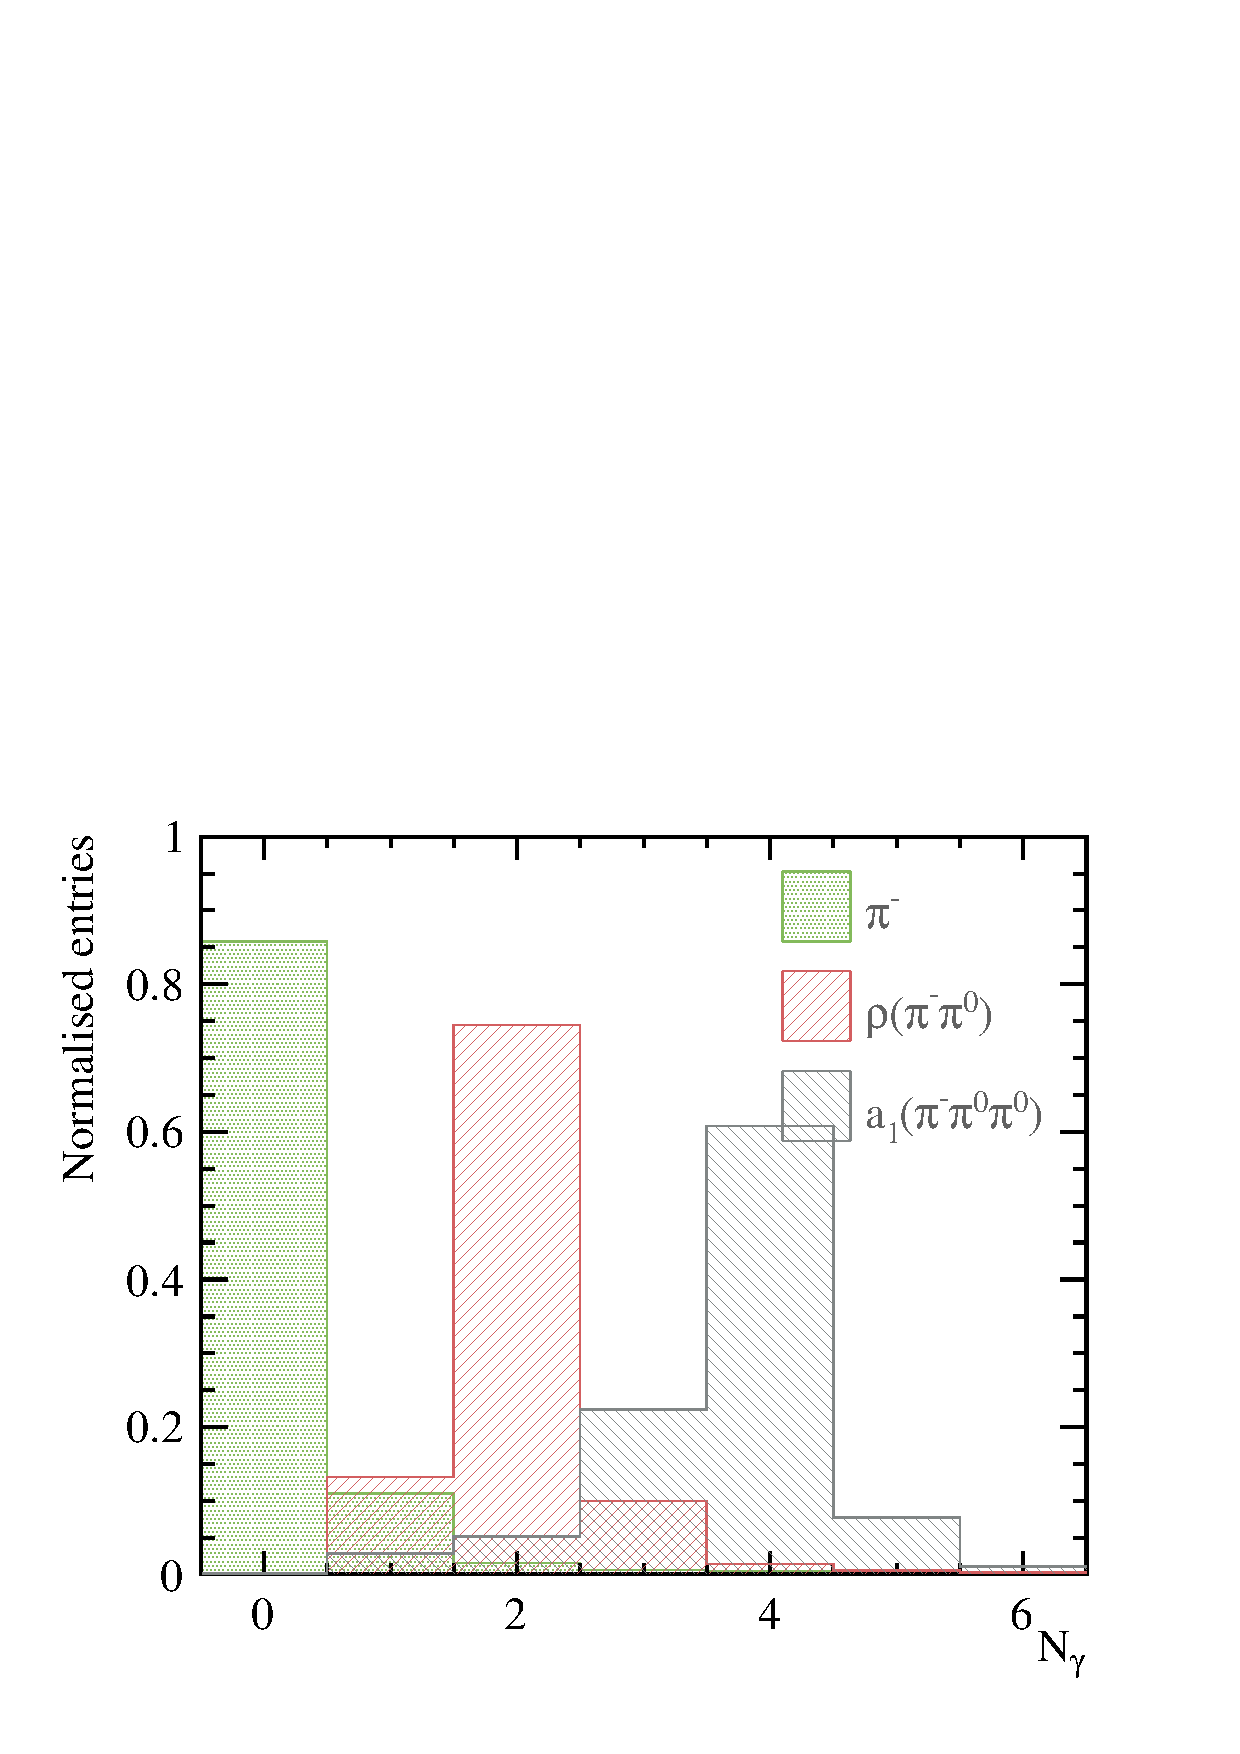
\includegraphics[width=\textwidth]{tau/var2/nPhoton_100GeV_improved.pdf}
  \caption{}
  \label{fig:tauVarNPhoton}
\end{subfigure}
\begin{subfigure}[b]{0.45\textwidth}
 \includegraphics[width=\textwidth]{tau/var2/mVis_100GeV_improved_zoom.pdf}
  \caption{}
  \label{fig:tauVarMVis}
\end{subfigure}
\begin{subfigure}[b]{0.45\textwidth}
 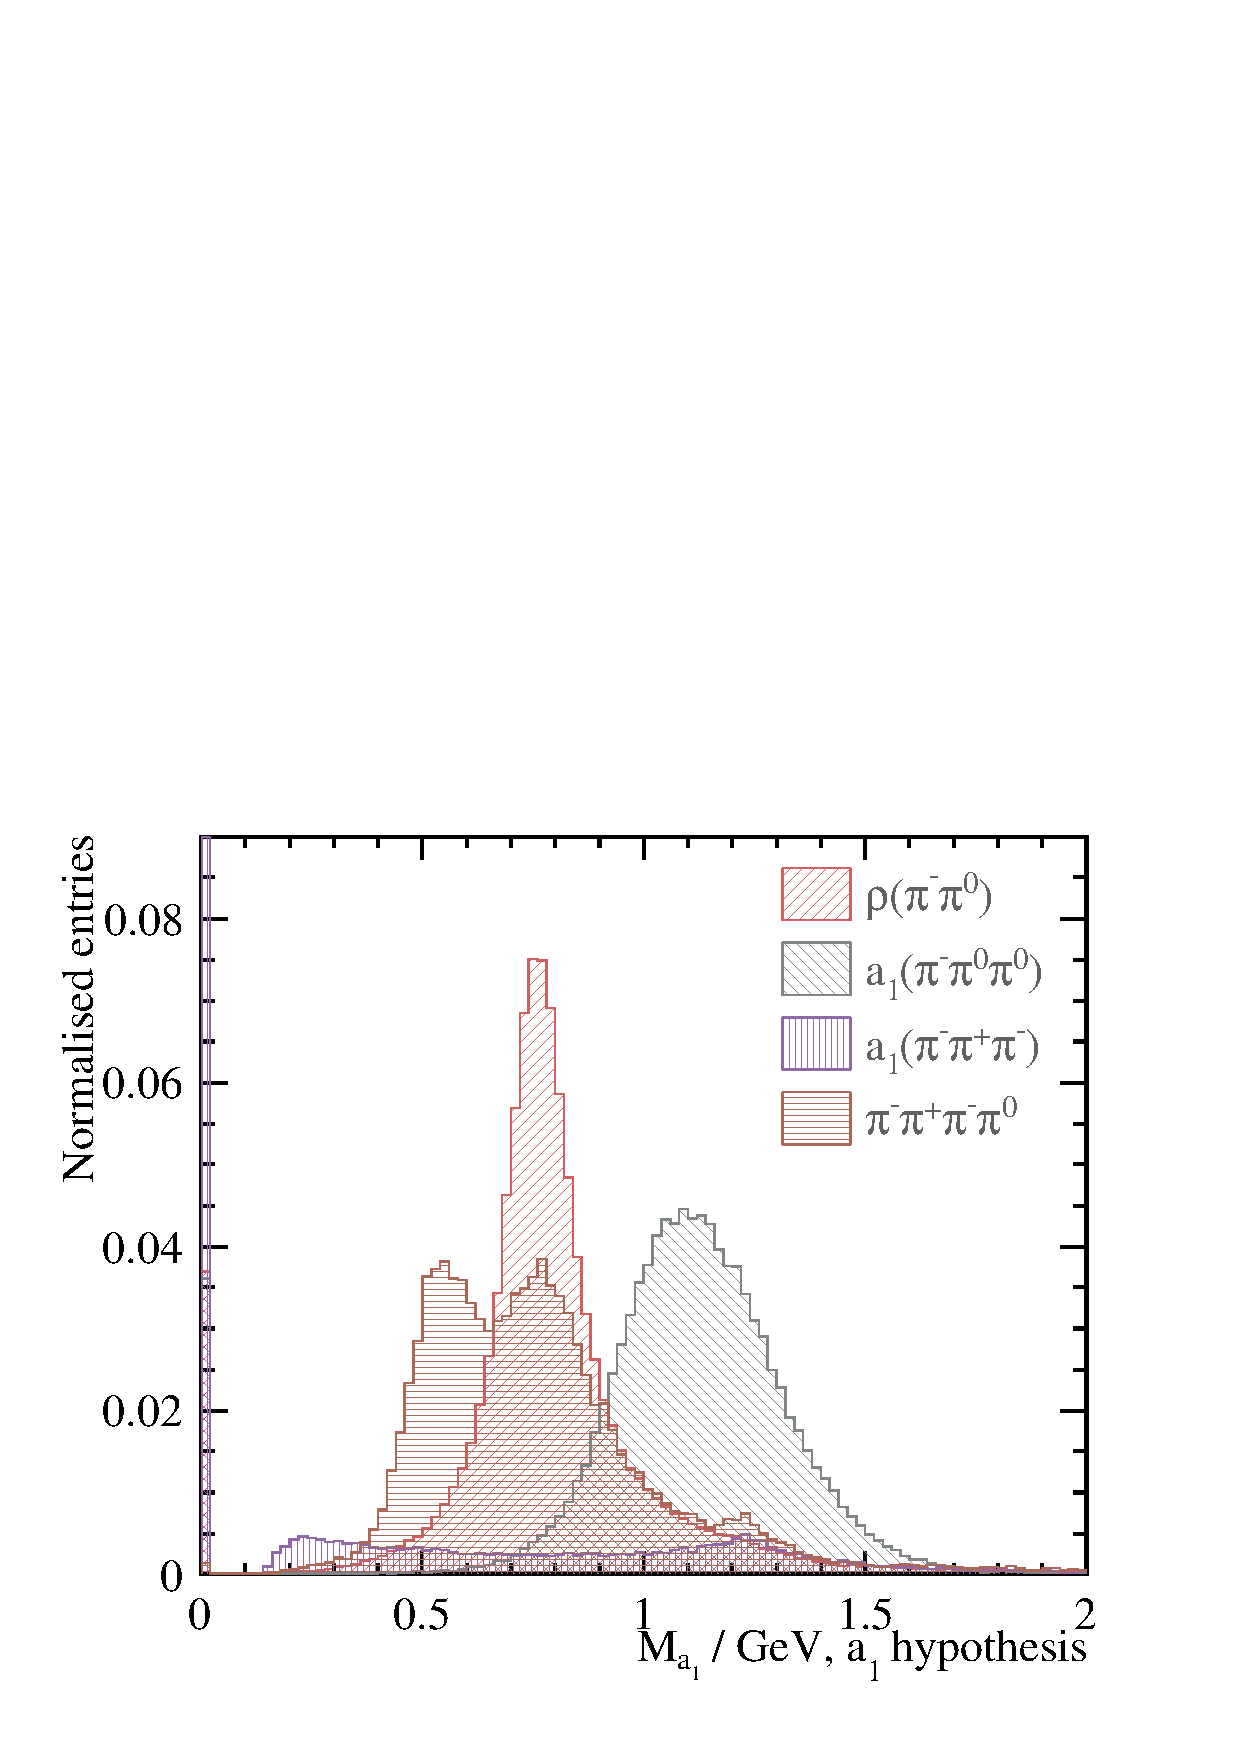
\includegraphics[width=\textwidth]{tau/var2/mA1A1Fit_100GeV_improved_zoom.pdf}
  \caption{}
  \label{fig:tauVarMA1}
\end{subfigure}

\caption
{Normalised distribution for a) the number of charged particle (${N}_{\charge}$); b) the number of photons (${N}_{\Pgg}$); c) the invariant mass of all visible decay products ($m_{vis}$); and d) the invariant mass of the \Pai, reconstructed with \decayAiPhotonShort hypothesis. Decay modes in all plots are selected with truth information.}
\label{fig:tauVar}
\end{figure}

\begin{table}[!htbp]\centering
\begin{tabular}{lr}
\hline
\hline
Category &  Variable \\
\hline
\PFOs number  & \multicolumn{1}{R{0.6\textwidth}}{  ${N}_{\charge}$, ${N}_{\Pmu}$, ${N}_{\Pe}$, ${N}_{\Pgg}$,  ${N}_{\Pgpm}$} \\
Invariant mass &  \multicolumn{1}{R{0.6\textwidth}}{$m_{vis}$, $m_{\charge}$, $m_{\neutral}$, $m_{\Pgg}$, $m_{\Pgpm}$} \\
Energy & \multicolumn{1}{R{0.6\textwidth}}{ $\tilde{E}_{vis}$,  $\tilde{E}_{\charge}$, $\tilde{E}_{\Pmu}$, $\tilde{E}_{\Pe}$, $\tilde{E}_{\Pgg}$,  $\tilde{E}_{\Pgpm}$} \\
Calorimetric info. &   \multicolumn{1}{R{0.6\textwidth}}{ $\% E_{\charge}$,  $\% E$ } \\
\decayRhoShort reconstruction & \multicolumn{1}{R{0.6\textwidth}}{  $m_{\Pgpz}\parenths{\rho}$, $m_\rho$} \\
\decayAiPhotonShort reconstruction &  \multicolumn{1}{R{0.6\textwidth}}{  $m_{\Pgpz}\parenths{\Pai}$, $m^*_{\Pgpz}\parenths{\Pai}$, $m_{\Pai}$} \\
EM shower profile & $\delta{l}$, $t_0$, $\langle{w}\rangle$ \\
Calorimeter hit info. & $\bar{E}_{hit}$, $\%MIP$ \\
Track info. & $\Delta E/P$ \\
\hline
\hline
\end{tabular}
\caption
{Variables used in the MVA event selection for the tau lepton decay mode classification.}
\label{tab:tauVaraibles}
\end{table}

\section{Multivariate Analysis}
\label{sec:tauMVA}
For the multivariate analysis, the multiclass class of the TMVA package \cite{Therhaag:2009dp} was used to perform a multiclass classification, which trains seven tau lepton decay final states simultaneously. The multiclass class is an extension of the standard two-class signal-background classifier. The discussion on multivariate analysis can be found in \Section{sec:pandoraMVA}. In particular the multiclass classifier is discussed in \Section{sec:pandoraMVAmulticlass}.

The multiclass classifier used is Boosted Decision Tree with Gradient boost (BDTG). The optimisation of the BDTG classifier follows the strategy in \Section{sec:pandoraMVAoptimisation}. The optimised parameters are listed in \Table{tab:tauBDTparameters}. An explanation of the variables can be found in \Section{sec:pandoraMVAbdtVar}.  Half of the randomly selected samples were used in the training process and the other half were used for testing.

\begin{table}[!tbp]\centering
%\small
\begin{tabular}{lr}
\hline \hline
 Parameter &  Value \\
\hline
Depth of tree & 5 \\
Number of trees & 3000 \\
Boosting & gradient boost \\
learning rate of the gradient boost & 0.1 \\
metric for the optimal cuts & Gini Index \\
bagging fraction & 0.5 \\
Number of bins per variables & 100 \\
End node output & yes/no \\
\hline \hline
\end{tabular}

\caption
{Optimised parameters for the Boosted Decision Tree with Gradient boost multiclass classifier. See \Section{sec:pandoraMVAbdtVar} for a detailed explanation of variables.}
\label{tab:tauBDTparameters}
\end{table}


\section{Classification Efficiency}

The Classification efficiencies for the seven tau decay modes are shown in \Table{tab:TauSelExample}. Bold numbers show the correct classification probability.

%For example, 99.8\% events of true \decayElectronShort decay mode are reconstructed correctly.

For the \decayElectronShort decay mode,   99.8\%  correct classicisation efficiency is achieved, due to variables dedicated to separation between \Pem and \Ppiminus. For \decayMuonShort decay mode,  99.5\% correct classicisation efficiency is achieved, due to efficient tracking detector and muon reconstruction algorithm.

For the \decayPionShort decay mode, 3.4\% events were classified as \decayRhoShortest decay mode. If the reconstruction is unable to reconstruct the photon pair from \Ppizero decay in \decayRhoShortest decay mode, the \decayPionShort and \decayRhoShortest decay modes would appear to  similar and misclassification is caused.

%The confusion with \decayElectronShort is at percent level, which is low due to the usage of EM shower variables. The percent level confusion with \decayAiPionShortest is because the tracking efficiency is at 98\%, where 2\% \decayPionShort events have more than one track reconstructed.

 %confusion with \decayRhoShortest decay mode  is to due to differentiate two event topologies. Around 15\% of \decayPionShort events have at least one photon reconstructed, mostly due to the FSR.

For the \decayRhoShortest decay mode, most misclassification comes from \decayAiPhotonShortest decay mode.  If the reconstruction is unable to resolve the all photon pair from \Ppizero decay in \decayRhoShortest and \decayAiPhotonShortest decay mode, the two decay modes would have similar topologies.

For the \decayAiPhotonShortest decay mode, the correct classification rate is the lowest among seven decay modes, as the \decayAiPhotonShortest decay final state is the most challenging to reconstruct correctly: two photon pairs and  one \Ppipm. The 9.5\% confusion with \decayRhoShortest is due to the same photon reconstruction failure issue. It should be noted that \Figure{fig:tauVarNPhoton} suggests that 30\% of \decayAiPhotonShortest events have fewer than four photons reconstructed, which overlaps with \decayRhoShortest distribution. The \decayAiPhotonShortest resonance reconstruction (\Section{sec:tauResonance}) and the multiclass classifier reduce the confusion between two final states  from 30\% to  9.5\%.

For the \decayAiPionShortest decay mode, the biggest source of misclassification  \decayThreePionPhotonShort decay, due to inability to resolve photons. The misclassification of  \decayThreePionPhotonShort decay mode  as \decayAiPionShortest decay mode is caused by the same reason.

%And the reason is the same for

%The unprecedented high classification rate has been achieved. The improvement of photon reconstruction described in \Section{} improved the ability to separate 1-prong final state. Most notably,  \Figure{} shows number of photons have a high correct reconstruction efficiency.


\begin{table}[htbp]
\centering
\small
\smallskip
\begin{tabular}{ l   r  r  r  r  r  r  r }
\hline
\hline
Reco$\downarrow$ Truth$\to$& \decayElectronShort & \decayMuonShort &\decayPionShort & \decayRhoShortest &\decayAiPhotonShortest &\decayAiPionShortest &\decayThreePionPhotonShort \\
\hline

{\decayElectronShort}&\textbf{99.7}\%&-&0.9\%&0.6\%&0.4\%&-&-\\
{\decayMuonShort}&-&\textbf{99.5}\%&0.6\%&-&-&-&-\\
{\decayPionShort}&-&0.3\%&\textbf{94.0}\%&0.8\%&-&0.4\%&-\\
{\decayRhoShort}&-&-&3.4\%&\textbf{93.6}\%&9.5\%&0.6\%&2.3\%\\
{\decayAiPhotonShort}&-&-&-&4.5\%&\textbf{89.7}\%&-&0.6\%\\
{\decayAiPionShort}&-&-&0.9\%&-&-&\textbf{96.8}\%&6.4\%\\
{\decayThreePionPhotonShort}&-&-&-&0.3\%&-&2.0\%&\textbf{90.6}\%\\

\hline
\hline
\end{tabular}

\caption[Classification efficiency for tau decay modes.]
{ Classification efficiency in percentage for tau decay modes using the nominal ILD detector model , for \rootSGeV{100}. Bold numbers show the correct classification probability. Numbers below 0.25\%, and \Pgngt are not shown in decay modes, for display purposes. Statistical uncertainties are less than 0.25\%.}
\label{tab:TauSelExample}
\end{table}




\section{Electromagnetic calorimeter  optimisation}
\label{sec:tauECAL}
In the above section, an analysis on tau decay mode classification is presented. Events used in the analysis are \eeToTauTau event at \rootSGeV{100} with nominal \ILD detector model. The analysis is repeated with varying \ECAL square cell sizes at 3, 5, 7, 10, 15 and 20\,mm, at four  \sqrtS = 100, 200, 500, 1000\,GeV. The multivariate classifier is trained for each cell size and each \sqrtS. Other \ECAL dimensions are kept the same as the \ILD nominal detector. Because the lepton reconstruction mostly relies on the tracking system, which is not varied in this study, only the  hadronic tau decays were investigated and compared between different \ECAL square cell sizes. In this way, the impact of the centre-of-mass energy and the \ECAL cell sizes on the classification efficiencies are studied. The correct classification efficiencies for  tau hadronic decay final states  as a function of the \ECAL square cell sizes for different centre-of-mass energies are shown in \Figure{fig:TauPionEfficiency}.


%The analysis is repeated with varying \ECAL square cell sizes at 3, 5, 7, 10, 15 and 20\,mm, at four  \sqrtS = 100, 200, 500, 1000\,GeV.


As \pandora is optimised for the nominal \ILD detector, a re-optimisation is required when changing the \ECAL square cell sizes. In particular, fragment removal algorithms have a large dependence on the \ECAL cell sizes. In particular, the \PhotonFragmentRemoval algorithm which merges photon fragments uses a distance metric. The optimised distance metrics as a function of the \ECAL square cell sizes are shown \Table{tab:TauPhotonFragmentRemovalParameter}. As cell sizes become larger, the distance cut for merging photons become larger.

\begin{table}[htbp]
\centering
%\small
%\smallskip
\begin{tabular}{ l   r  r  r  r  r  r  }
\hline
\hline
\ECAL square cell size & 3\,mm & 5\,mm & 7\,mm & 10\,mm & 15\,mm & 20\,mm  \\
\hline
ClosestHitDistance & 5 & 10 & 10 & 10 & 20 & 20 \\
\hline
\hline
\end{tabular}

\caption[Optimised parameters of \PhotonFragmentRemoval algorithm as a function of \ECAL square cell size.]
{Optimised parameters of \PhotonFragmentRemoval algorithm as a function of \ECAL square cell size.}
\label{tab:TauPhotonFragmentRemovalParameter}
\end{table}

The increase in the centre-of-mass energies  would boost photons. The photon pair would be more collimated, and therefore be more challenging to separate. The inability to separate photon pairs will degrade the classicisation performance.

The change in the \ECAL cell size will change the transverse spatial resolution. Hence a large cell size will result in a low transverse spatial resolution, and leading to inability to separate photon pairs. Consequently, a worse classification performance is expected for a larger \ECAL cell size.


In general,  tau decay mode correct classification efficiencies generally decreases with increase of \sqrtS and increase of \ECAL cell sizes, as expected. This trend is observed for almost all tau decay modes. As the centre-of-mass energy increases, tau decay products are often boosted. It is increasingly difficult to separate decay products. For example, the photon pair from \Ppizero decay becomes very challenging to separate at a high centre-of-mass energy. Increase of the \ECAL cell sizes has a similar effect. With a bigger cell size, multiple photons may deposit energy in a same cell, making separating these photons  almost impossible.

For the \decayPionShort decay mode, the general trend is followed. The efficiency for \rootSGeV{200} is slightly better than that of the \rootSGeV{100} for small cell sizes.

For the \decayRhoShort decay mode,the efficiency for  \rootSGeV{500} increases as the cell sizes increases. This is because the multivariate classifier optimises for the overall classification efficiency, which may compensate one decay mode for another. In this case, the small increase in efficiency for \decayRhoShort at \rootSGeV{500} is compensated by the drastic decrease in efficiency for \decayAiPhotonShort at  \rootSGeV{500}.

For the \decayAiPhotonShort decay mode, the loss of efficiency with an increasing  cell size and increasing centre-of-mass energy is most significant comparing to other decay modes. With most number of particles in the final state, it is the most challenging decay channel to reconstruct and thus most sensitive to the change in cell sizes and centre-of-mass energy.

For the \decayAiPionShort decay mode, the efficiencies are similar to that of the \decayPionShort. Both final states contain charged particles only. Therefore it is most sensitive to the tracking performance, which is not affected by varying the \ECAL cell sizes.

For the \decayThreePionPhotonShort decay mode, the decrease in efficiencies are more significant for \rootS{500} and 1000\,GeV.

The leptonic decay  correct reconstruction efficiency is not used as a metric as they are similar across different \ECAL cell sizes. This is because the \Pepm and \Pgmpm identifications mostly rely on the tracking system, which was not varied in this study. The energy deposited in the calorimeter are used for the association to the tracks but it has a small impact on the lepton identification.
%This classification can be applied for different  \sqrtS and with different detector models. The main reconstruction issue is to separate boosted photon pair from \Ppizero decay. High \sqrtS The \ECAL cell size is crucial in separating the EM showers from photons. As discussed in previous chapter, separating photons requires a high transverse spatial resolution. Therefore, the \ECAL square cell size is expected to affect the classification efficiency.

%The main difficulty in the classification is to classify 1-prong final states.  These final states involves \Ppizero, where two photons from \Ppizero decay could be poorly reconstructed. At high energy, \Ppizero is boosted making the reconstruction more challenging. The ability to reconstruct the two photons as separate entities requires good pattern recognition algorithm for photons and \ECAL spatial resolution. Hence the improved photon reconstruction in \Chapter{chap:Photon} is used in this study. The impact of the \ECAL transverse spatial resolution on the tau decay classification is demonstrated as well.





%\FIGURE{fig:TauPionEfficiency} shows the correct classification efficiencies for  tau hadronic decay final states  as a function of the \ECAL square cell sizes. For example, plotted values for 5\,mm cell size at \rootSGeV{100} are the same as the bold numbers in \Table{tab:TauSelExample}.




\begin{figure}[htbp]
\centering % \begin{center}/\end{center} takes some additional vertical space
\begin{subfigure}[b]{0.45\textwidth}
  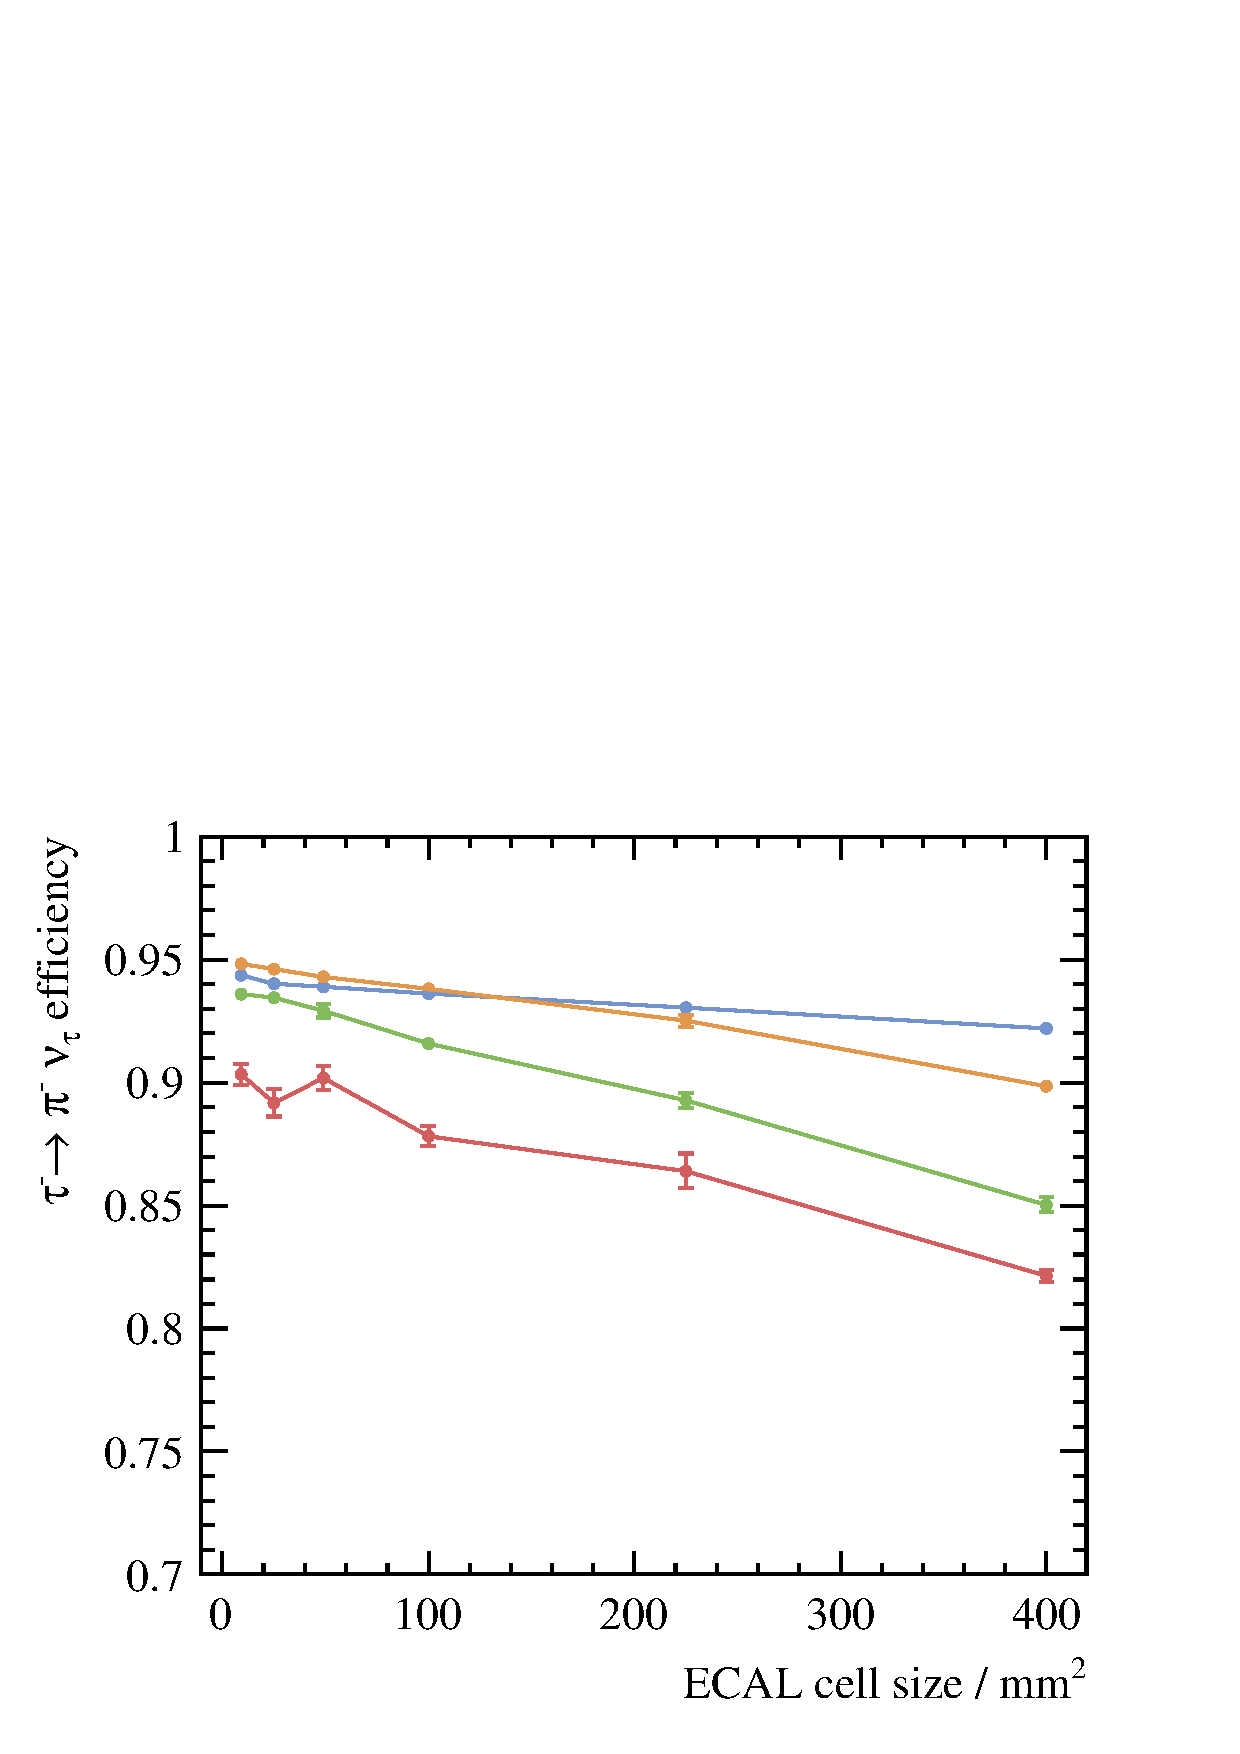
\includegraphics[width=\textwidth]{tau/plots3/decayMode2.pdf}
  \caption{}
  \label{fig:tauDecayMode2}
\end{subfigure}
\begin{subfigure}[b]{0.45\textwidth}
  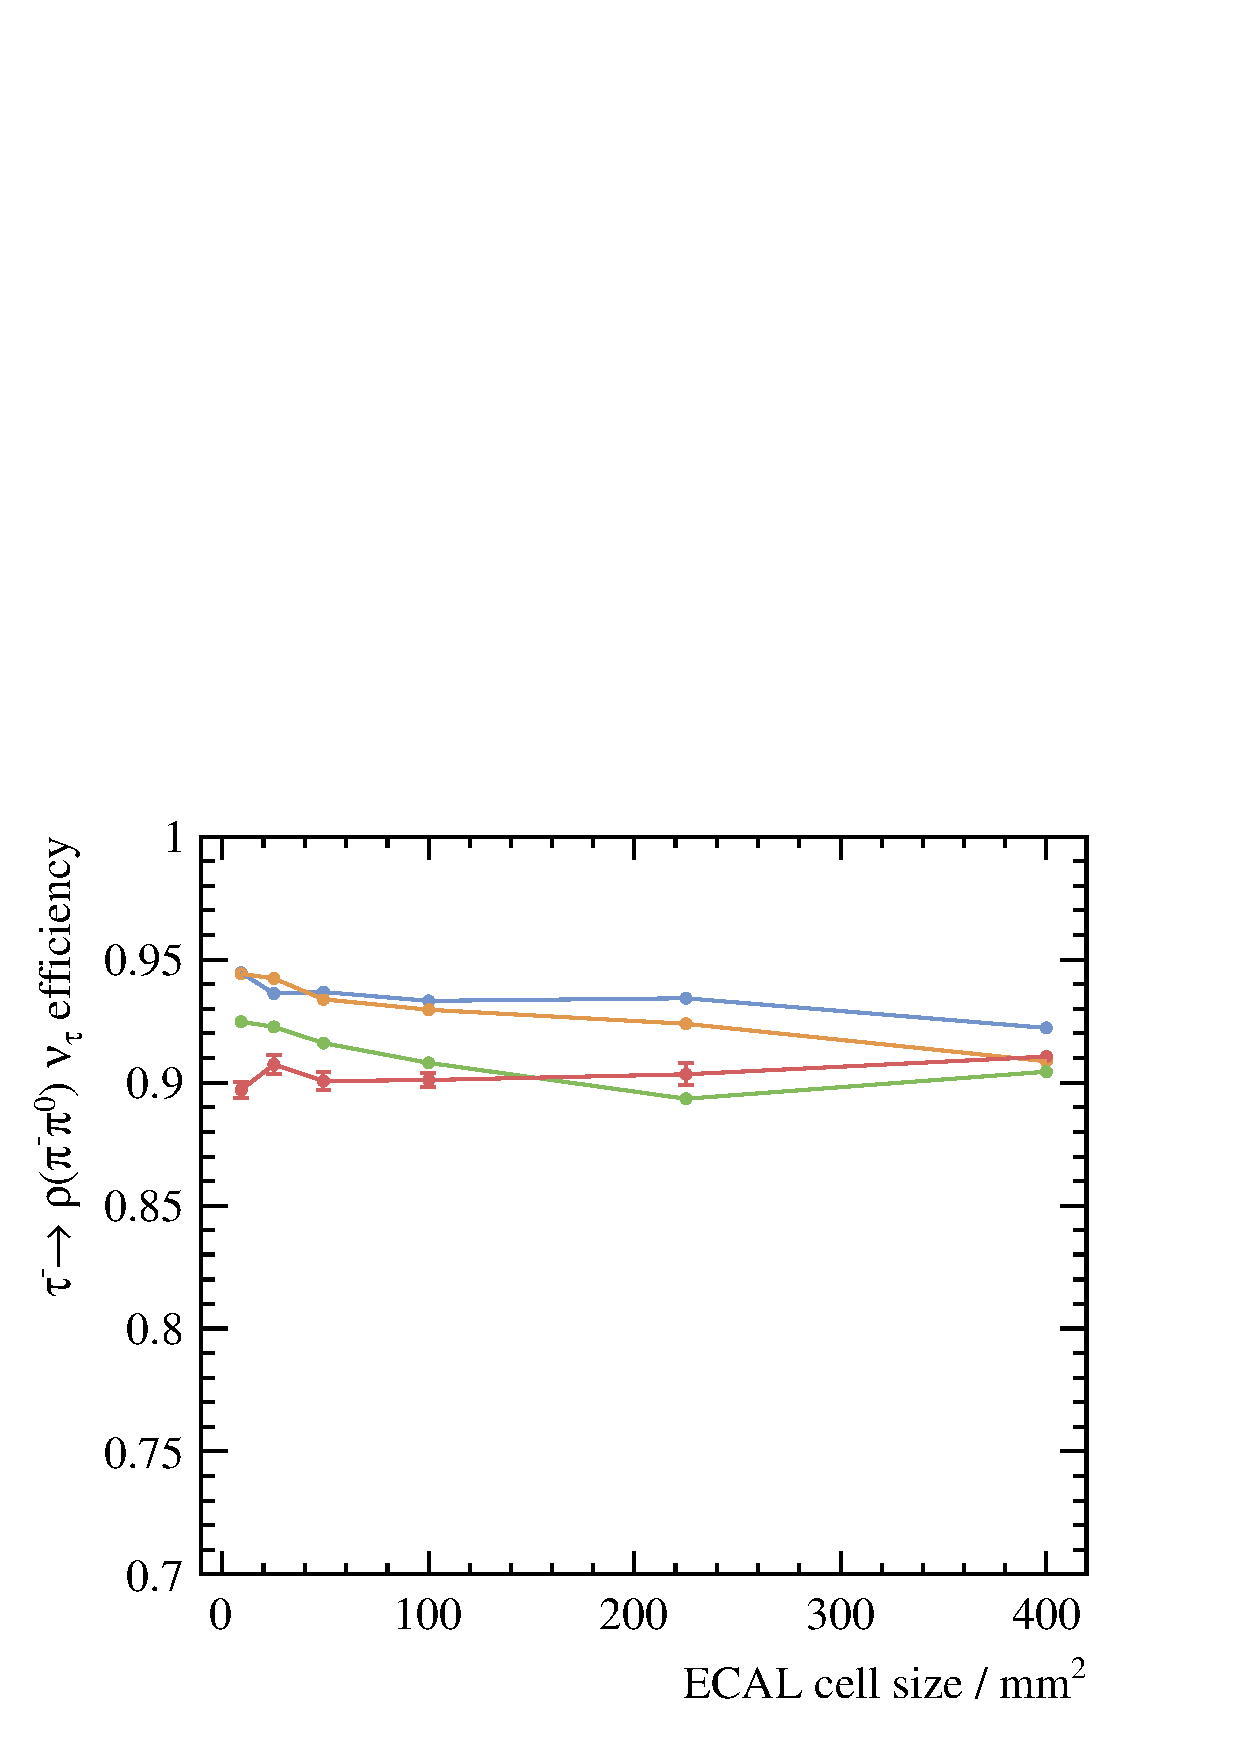
\includegraphics[width=\textwidth]{tau/plots3/decayMode3.pdf}
  \caption{}
  \label{fig:tauDecayMode3}
\end{subfigure}
\begin{subfigure}[b]{0.45\textwidth}
  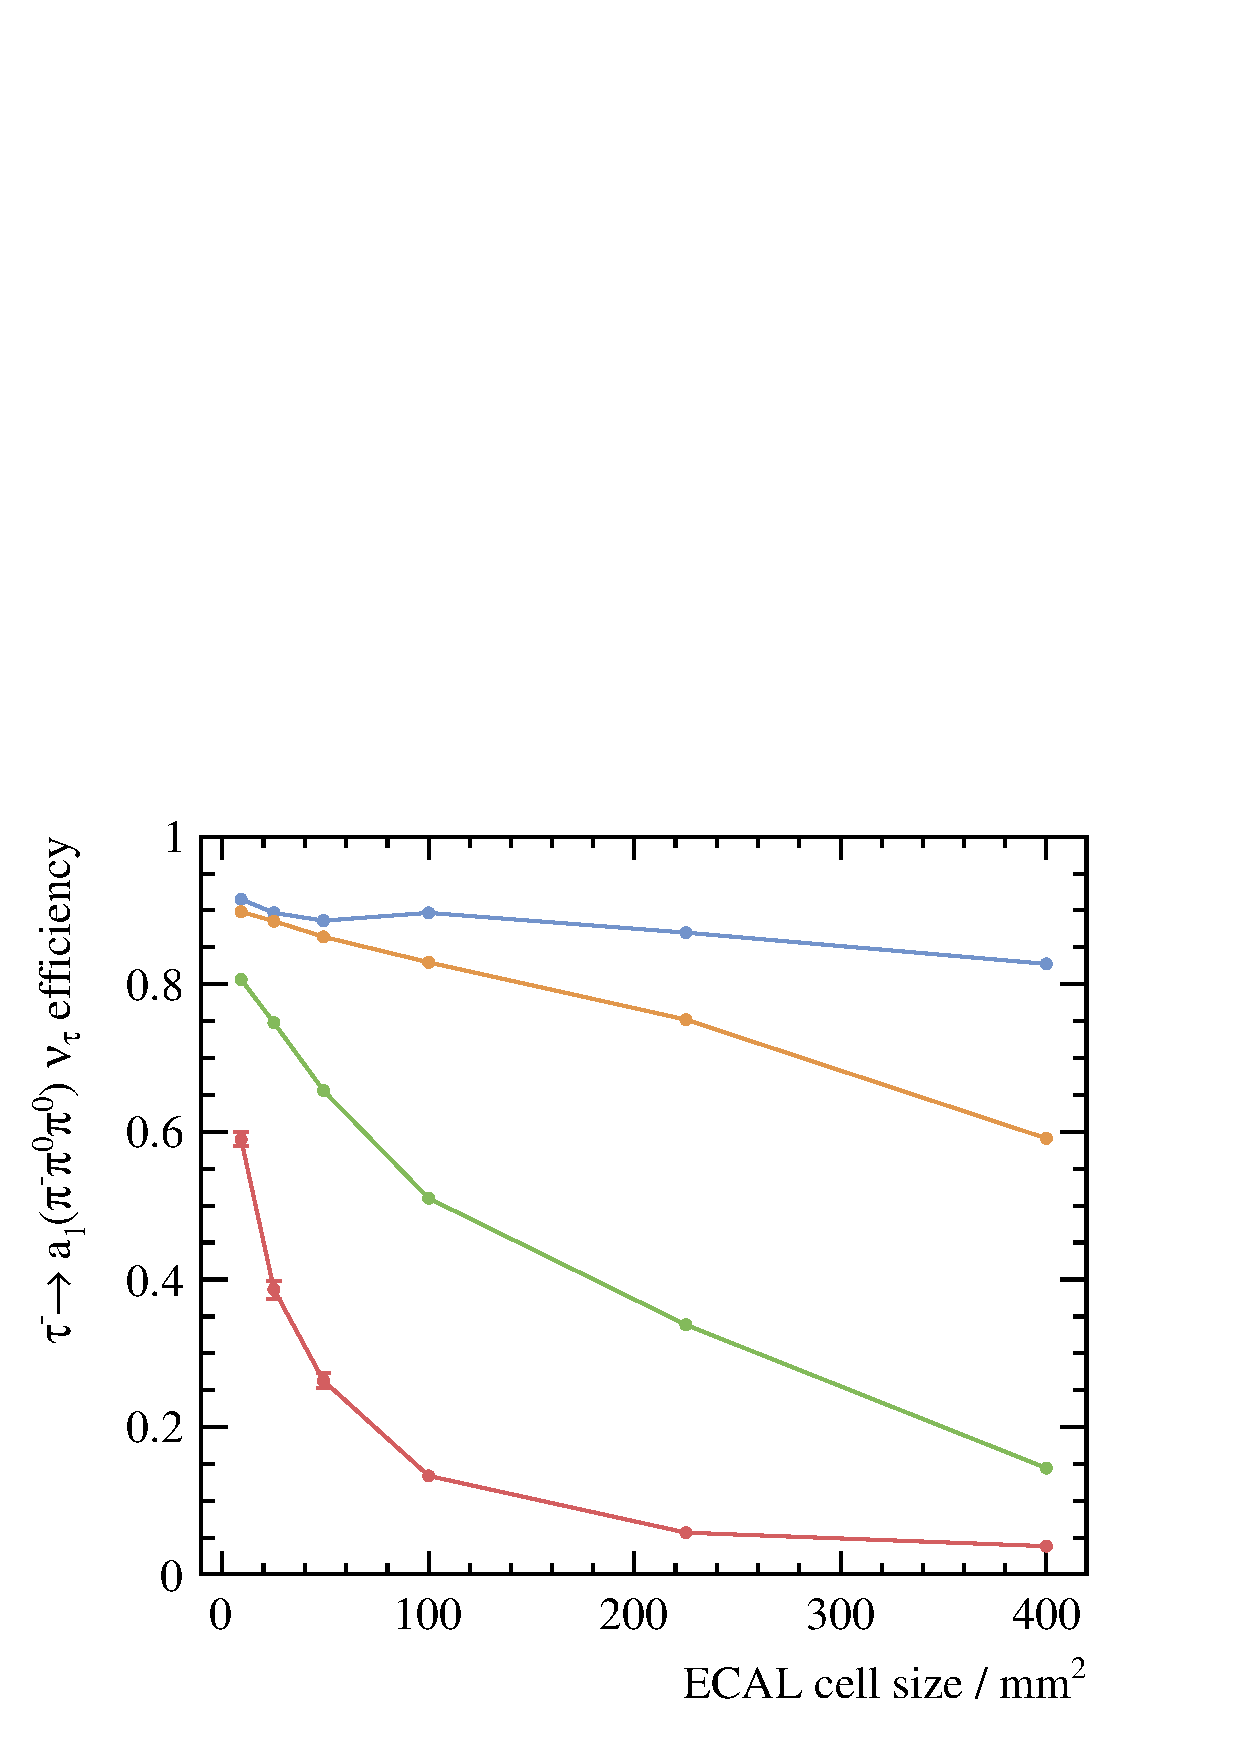
\includegraphics[width=\textwidth]{tau/plots3/decayMode4.pdf}
  \caption{}
  \label{fig:tauDecayMode4}
\end{subfigure}
\begin{subfigure}[b]{0.45\textwidth}
  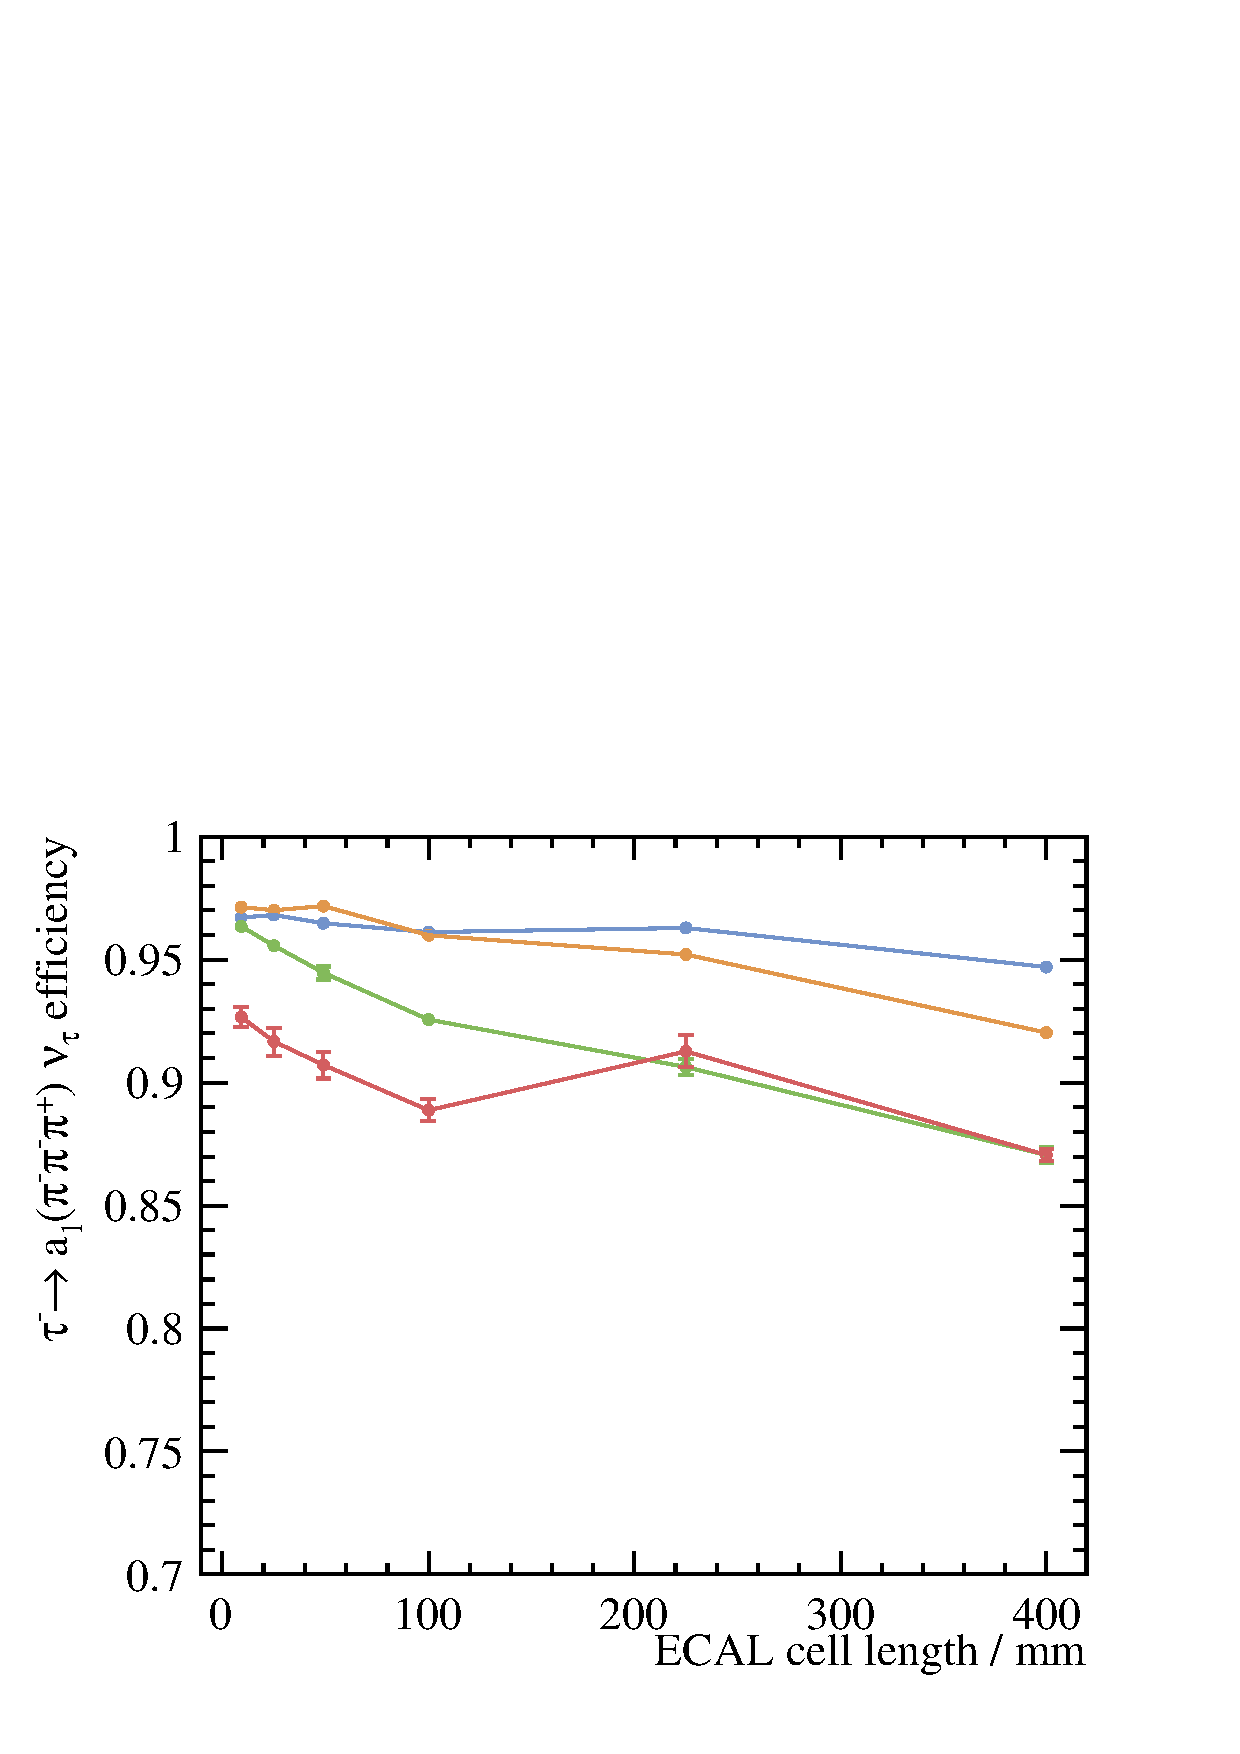
\includegraphics[width=\textwidth]{tau/plots3/decayMode5.pdf}
  \caption{}
  \label{fig:tauDecayMode5}
\end{subfigure}
\begin{subfigure}[b]{0.45\textwidth}
  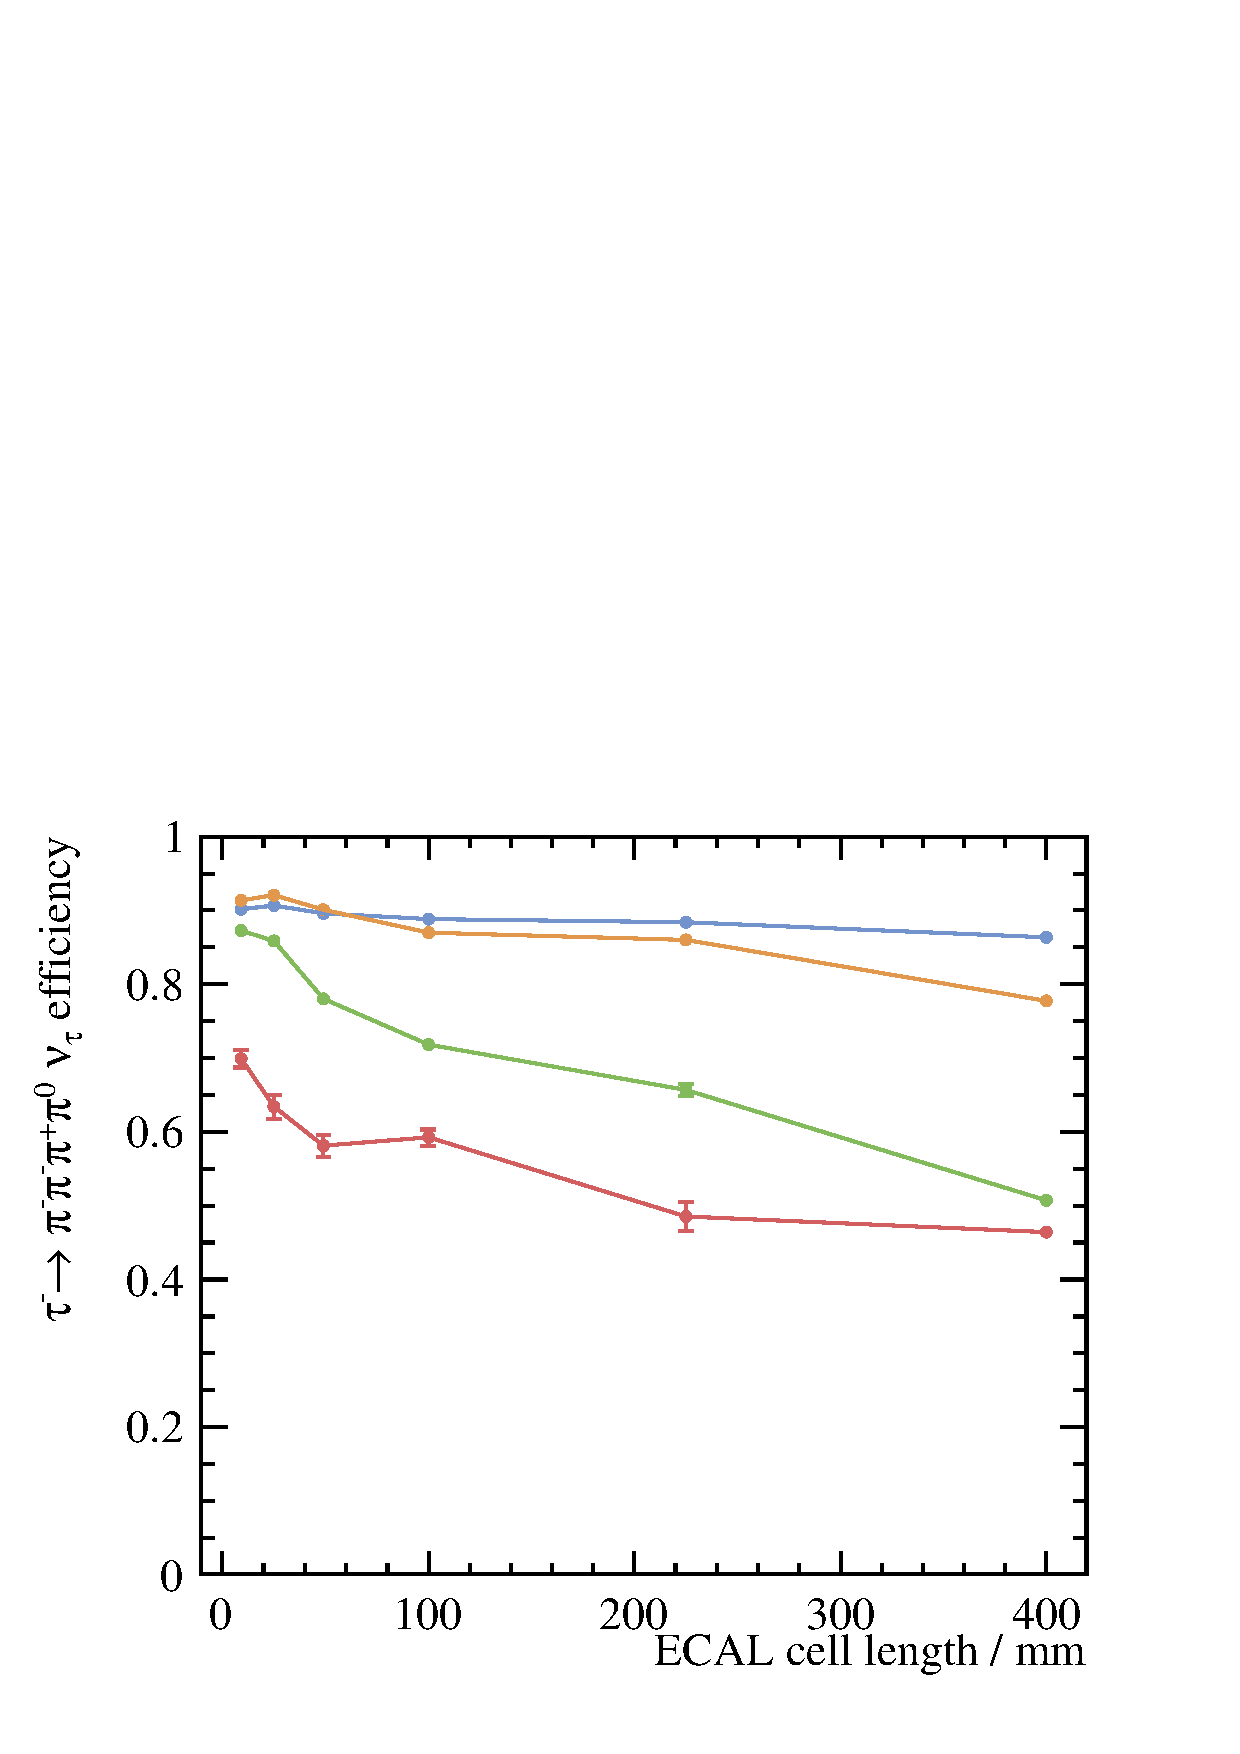
\includegraphics[width=\textwidth]{tau/plots3/decayMode6.pdf}
  \caption{}
  \label{fig:tauDecayMode6}
\end{subfigure}
\begin{subfigure}[b]{0.45\textwidth}
  \includegraphics[width=\textwidth]{tau/plots3/legend.pdf}
  \caption{}
  \label{fig:tauDecayLegend}
\end{subfigure}
\caption[The correct classification efficiency for  tau hadronic decay final states  as a function of the \ECAL square cell sizes]
{ The correct classification efficiencies for  tau hadronic decay final states  as a function of the \ECAL square cell sizes for a) \decayPionShort decay mode, b) \decayRhoShortest decay mode, c) \decayAiPhotonShortest decay mode, d) \decayAiPionShortest decay mode, and e) \decayThreePionPhotonShort decay mode. The legend is shown in f). All plots are produced using  the \ILD detector model with \sqrtS = 100, 200, 500 and 1000\,GeV.}
\label{fig:TauPionEfficiency}
\end{figure}


\subsection{Tau hadronic decay correct classification efficiency}

There are two reasons for constructing a single parameter for the overall Tau decay efficiency. Firstly the multivariate classifier is trained to optimised to achieve the best the overall classification efficiency. Secondly it is easier to compare the impact of different detector models and different \sqrtS. The choice of neglecting the tau leptonic  decay  is because reconstructing hadronic decays is sensitive to the \ECAL cell sizes, which is relevant for this study.

The constructed tau hadronic decay correct classification efficiency, \tauHad, is a weighted classification efficiency for all hadronic decay modes:
\begin{equation}
\label{eq:had}
\tauHad = \frac{\sum_{i}^5 {Br}_{i}\varepsilon_{i}}{\sum_{i}^5 {Br}_{i}}  \,,
\end{equation}
where $Br_{i}$ is the branching fraction of the hadronic decay mode $i$  after the generator level cut (\Section{sec:tauPreSel}); $\varepsilon_{i}$ is the correct reconstruction efficiency of the decay mode $i$; and $i$ is summing over five tau hadronic decay modes.

\FIGURE{fig:TauHadronicEfficiency} shows \tauHad as a function of \ECAL cell sizes with increasing centre-of-mass energies. The general trend for the \tauHad is that \tauHad decreases with increase of \sqrtS and increase of \ECAL cell sizes for the same reasons stated in the previous section. 

%As the \sqrtS increases, tau decay products are boosted and it is challenging to separate identical decay products. Similarly,  increasing \ECAL cell sizes makes particle separation more difficult.

For \tauHad at \rootSGeV{100}, the efficiency decreases from 94\% at 3\,mm cell size, to 91\% at 20\,mm cell size. The decrease is approximately proportional to the increase in the cell size.

For \tauHad at \rootSGeV{200}, the efficiency decreases from 94\% at 3\,mm cell size, to 86\% for a \ECAL cell size of  20\,mm.
%There is a large decrease from 15\,mm to 20\,mm cell size.

For \tauHad at \rootSGeV{500}, the efficiency decreases from 92\% at 3\,mm cell size, to 78\% at 20\,mm cell size. Most significant decrease occurs at this \sqrtS.

For \tauHad at \rootSGeV{1000}, the efficiency decreases from 85\% at 3\,mm cell size, to 75\% at 20\,mm cell size.
%From 10\,mm cell size onwards, the \tauHad decrease slows down.

The increase in \ECAL cell sizes has a larger impact at high centre-of-mass energies. With decay products spatially close at high centre-of-mass energies, it is more beneficial to have a smaller \ECAL cell size to reconstruct individual particle.

\begin{figure}[htbp]
\centering % \begin{center}/\end{center} takes some additional vertical space
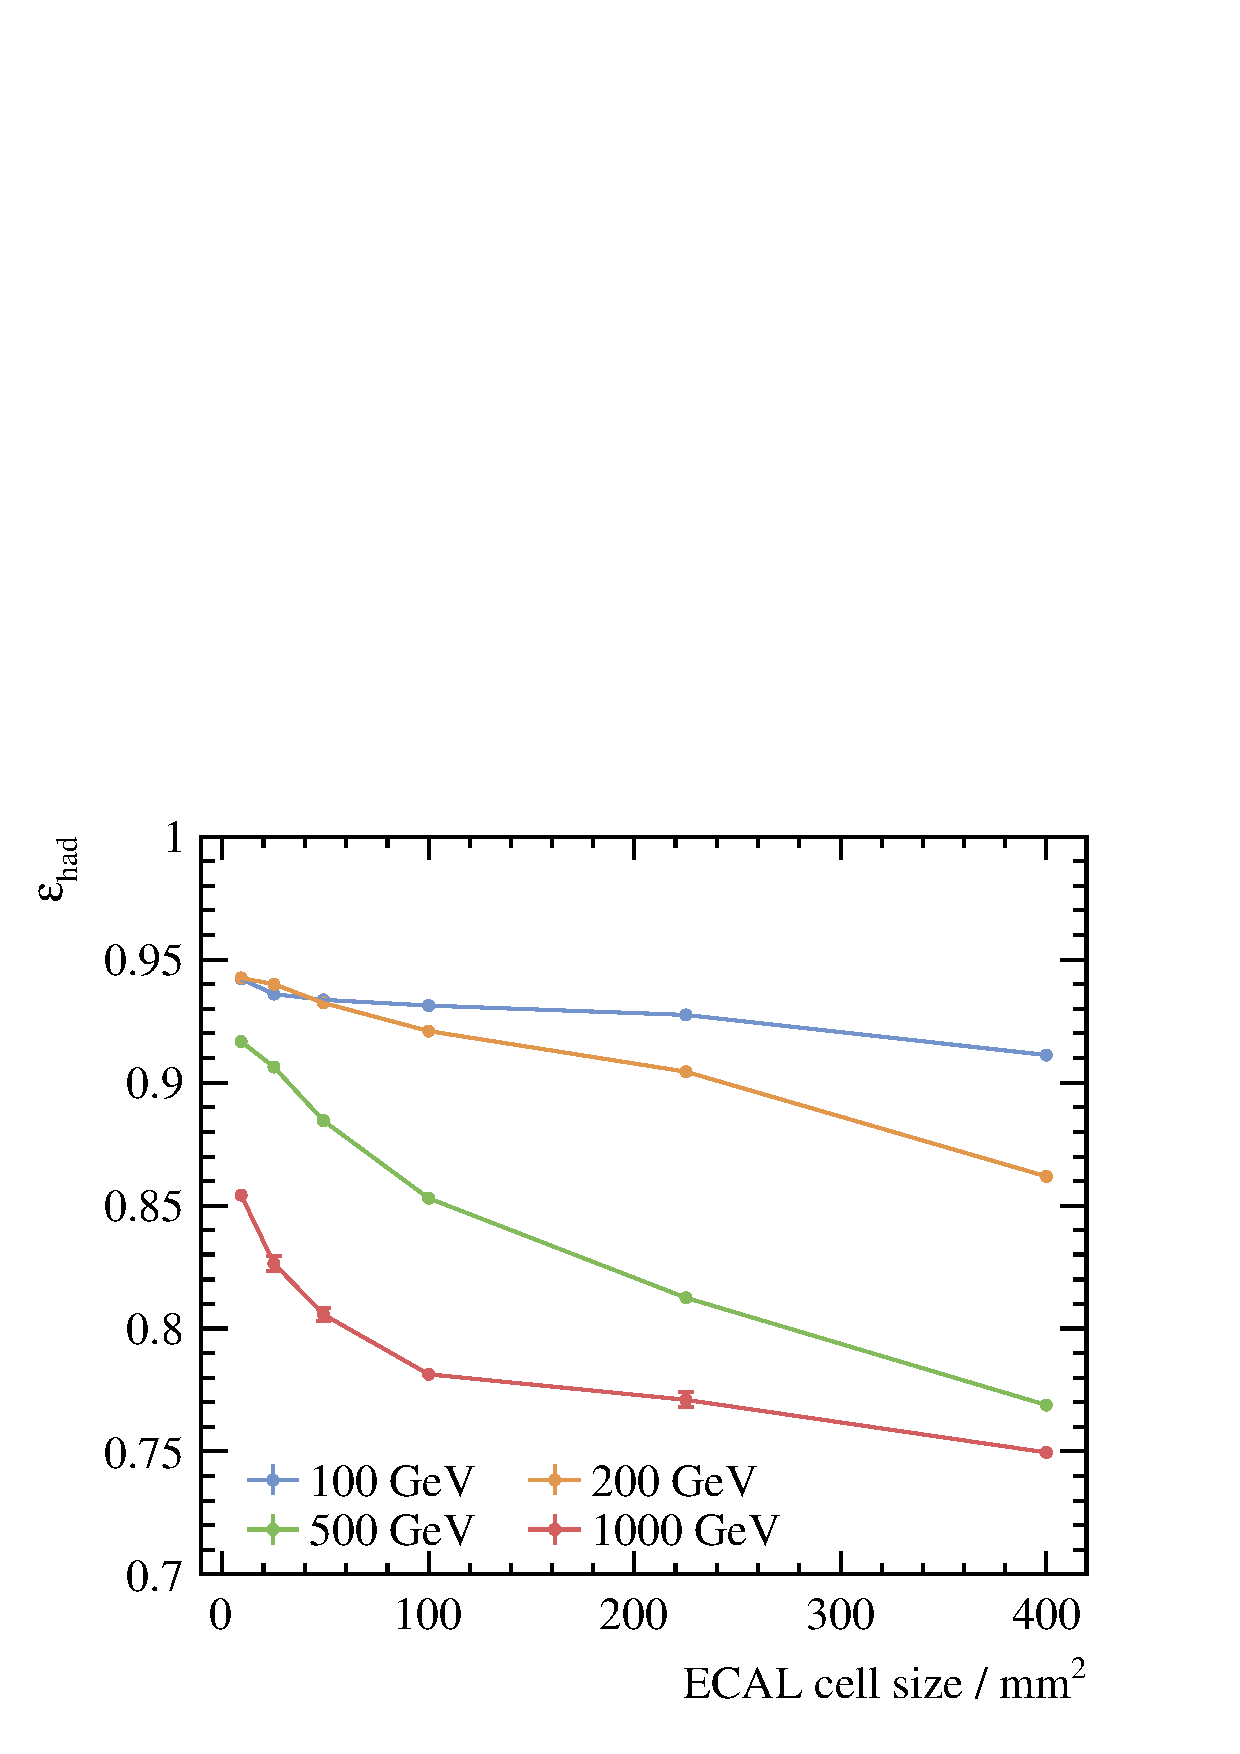
\includegraphics[width=.85\textwidth]{tau/plots3/hadronicEff.pdf}
\caption[The tau hadronic decay efficiency as a function of  the \ECAL cell sizes at different \sqrtS with the \ILD detector model.]
{The tau hadronic decay efficiency, \tauHad, as a function of  the \ECAL cell sizes at different \sqrtS with the \ILD detector model. The blue, orange, green and red lines are representing the analysis at \sqrtS = 100, 200, 500 and 1000\,GeV respectively.}
\label{fig:TauHadronicEfficiency}
\end{figure}


\section{Separating \PHiggs from \PZ with tau pair decay}
\label{sec:tauHZ}
\PHiggs can be separated from  \PZ using  tau pair decay channel.  The difference in the spin of the boson reflects in the different polarisation correlation of the tau pair. By extracting the polarisation correlation, parent bosons can be separated. A proof-of-principle analysis is presented to demonstrate the usage of the tau decay mode classification, motivated by theoretical studies such as in \cite{Bullock:1991my}. The theoretical motivation is described in \Section{sec:theoryTauPair}. The subsequent sections discuss the ability to reconstruct the polarisation correlation of the \PZ using tau pair decay, and to match with the truth information.

The analysis largely follows the same procedure for the tau decay mode classification. Differences are highlighted in sections below.

The channel is \HepProcess{\Pep \Pem \to \PZ \PZ}, where one \PZ decays hadronically and the other \PZ decays to a tau lepton pair. The samples were generated at \rootSGeV{350} without \ISR contribution for this proof-of-principle study.

\subsection{Event pre-selection}

The same seven tau decay modes in \Section{sec:tauDecayModes} are studied. The \tauToPion decay mode is selected to demonstrate tau pair polarisation correlation, and to complete the proof-of-principle analysis of \PHiggs / \PZ separation with tau pair decay channel.

The event pre-selection is similar to that in \Section{sec:tauPreSel}. The cut on the visible energy of decay products is not used, because a large fraction of \ZToTauTau events, where \tauToPion, have two low-energy charged pions. Therefore, the cut on the visible energy of decay products would bias the distribution.


\subsection{Identifying tau pairs}

The final state of \HepProcess{\Pep \Pem \to \PZ \PZ} channel contains two tau leptons and two quark jets. Therefore, tau decay products can either be found by direct tau searching, or by finding two jets and assigning the recoil momenta to the two tau system. If a tau lepton decays into a few particles, then the direct tau searching would work better. If a tau lepton decays into many particles, finding tau decay products as a jet has a better performance, as jet clustering works better with more particles. Hence, two approaches are combined for the best tau pair identification.

\subsubsection{Direct tau search}
Tau finder processer, \BonoTauFinder is a modified version of the one in \Section{sec:doubleHiggsBonoTauFinder}. The basic idea is to find tau decay products consistent with decay topologies, and requires the tau  decay products to be isolated from the rest of the particles in an event. Parameters chosen are set to find as many as possible tau candidates. 
%The filtering of the candidates is via kinematic constraints.
The modified \BonoTauFinder works as following. Particles with transverse momentum less than 0.5\,GeV are not considered. A seed particle is chosen and a search cone is formed around the seed, which requires one or three tracks with the invariant mass  of all particles inside the search cone less than 3\,GeV. The isolation criteria states that the opening angle between the search cone  and the $2^{nd}$ closest track is larger than 0.6\,rad. If the criteria is satisfied,  the search cone with the tau seed is identified as a tau lepton.

\begin{table}[!htbp]
\begin{tabular}{lr}
\hline
\hline
Modified \BonoTauFinder  & Selection \\
\hline
Veto low \pT &  $\pT < 0.5$\,GeV\\
Seed particle & $\pT > 1$\,GeV \\
Maximum search cone opening angle  & $\theta_S \leqslant \cos^{-1}(0.99)$\\
Tau candidate rejection & $N_{X^+} \neq 1,3$, $m_{PFO} > 3$\,GeV   \\
Isolation & $\theta_{cone,2^{nd}X^+} > 0.6$\,rad\\
\hline
\hline
\end{tabular}
\caption
{Optimised parameters of modified \BonoTauFinder.}
\label{tab:tauBonoTauFinderProcessor}
\end{table}

\subsubsection{Jet clustering}

Tau hadronically decay can be also identified as a small jet. The Durham algorithm \cite{Catani:1991hj} was used to jet clustering, also known as the \ee \kt algorithm. (see \Section{sec:pandoraJetDurham}). The jet algorithm runs in the exclusive mode to find four jets.

\subsubsection{Select tau candidates}

The best tau pair candidates are selected using kinematic constraints. In the \HepProcess{\Pep \Pem \to \PZ \PZ}, the energy of the \PZ is half of the centre-of-mass energy. The invariant mass of two quarks from \PZ should be close to \PZ mass. Therefore, the minimisation function is
\begin{equation}
\chi^2 = \frac{\parenths{m_{\Pquark\Pquark} - m_{\PZ}}^2}{\sigma_{m_{\Pquark\Pquark}}^2} + \frac{\parenths{E_{\Pquark\Pquark} - \frac{\sqrtS}{2}}^2}{\sigma_{E_{\Pquark\Pquark}}^2},
\label{eq:tauMinimiser}
\end{equation}
where $m_{\PZ}$ is the mass of \PZ from reference \cite{Agashe:2014kda}; $\sigma_{m_{\Pquark\Pquark}}$ and $\sigma_{E_{\Pquark\Pquark}}$ are the reconstructed mass resolution  and energy resolution of the \PZ, respectively; and $m_{\Pquark\Pquark}$ and  $E_{\Pquark\Pquark}$ are defined differently for the direct tau searching and the jet clustering method. For the direct tau search method, $m_{\Pquark\Pquark}$ and  $E_{\Pquark\Pquark}$ are defined as the recoil momenta against two tau candidates by iterating over all  tau candidates, assuming collision at \sqrtS. For the jet clustering method,  $m_{\Pquark\Pquark}$ and  $E_{\Pquark\Pquark}$ are defined as the mass and energy of two jets by iterating over all possible jets.

The $\chi^2$ minimiser is repeated for the direct tau search method and the jet clustering method. Each method choose a best tau pair candidate with a smallest $\chi^2$. Hence two tau pair candidates with $\chi^2$ are obtained. To find the overall best tau candidate, a set of conditions is used. If the best tau pair candidate for both methods satisfies the kinematic constraint:
\begin{equation}
\absOf{m_{\Pquark\Pquark} - m_{\PZ}} < \sigma_{m_{\Pquark\Pquark}}\ , \absOf{E_{\Pquark\Pquark} - \frac{\sqrtS}{2}} < \sigma_{E_{\Pquark\Pquark}},
\label{eq:tauMinimiserSelector}
\end{equation}
the  tau pair candidate  with smallest $\chi^2$ is selected. Otherwise, if only one candidate satisfies the constraint in \Equation{eq:tauMinimiserSelector}, that candidate is chosen. If none of the candidates satisfies the constraint, and if one jet from the jet clustering is close to the beam pipe and there are exactly two tau leptons from \BonoTauFinder, then these two tau leptons are chosen. This is due to the fact that if one jet is close to the beam pipe, it is likely that some particles close to the jet are undetected, which leads to a failure in the kinematic constraint. Lastly, if all conditions above are not satisfied, two smallest jets by the number of \PFOs are chosen to be tau leptons decay products.

\subsection{Boost to \PZ decay rest frame}

The previous section describes the method to identify the tau pair decay products.  To use the tau decay mode classifier, it is necessary to know the tau lepton energy. For the channel \HepProcess{\PZ \to \APtauon \Ptauon}, the  energy of the tau lepton can be calculated in \PZ decay rest frame, which is half of the \PZ energy in the rest frame. The next step is to calculate the energies of tau decay products in the rest frame. The decay products are boosted to the \PZ decay rest frame, which requires the \fourMomentum of the \PZ.

The \fourMomentum of the \PZ decaying to tau pair is calculated from the recoil momenta of non tau-decay-products:
\begin{equation}
p^{\mu}_{\Ptau\Ptau} =
  \begin{pmatrix}
    \sqrtS\\   \sqrtS\times\sin\parenths{\theta_{beam}}\\  0   \\       0 \\
  \end{pmatrix}
  - \sum_{i}^{non-\Ptau}p^{\mu}_{i},
\end{equation}
where $\theta_{beam}$ is the beam crossing angle and index $i$ is summing over all non-tau-decay-product \PFOs. Extra kinematic constraint fixes the energy of the $p^{\mu}_{\Ptau\Ptau}$ to be half of \sqrtS:
\begin{equation}
p^{\mu}_{\Ptau\Ptau,correct} \equiv p^{\mu}_{\Ptau\Ptau} \times \frac{\frac{1}{2}\sqrtS}{E_{\Ptau\Ptau}}.
\end{equation}
$p^{\mu}_{\Ptau\Ptau,correct} $ is used as the boost vector to boost tau decay products in the rest frame. The calculation of the variables for the MVA classifier are performed in the \PZ decay rest frame.

\subsection{Variables used in the MVA}

Variables used in  the MVA classifier are a subset as the ones used in the previous analysis, listed in \Table{tab:tauVaraibles}. Variables regarding EM shower profiles, calorimeter hit information and track information are not used (last three rows in \Table{tab:tauVaraibles}) as the study focuses on the overall tau decay mode separation.

%Also for the computational reason, it was not feasible to use these variables for the MVA. \Pep and \Ppiplus separation could be improved if these extra variables are included.


\subsection{Multivariate analysis}

Half of the sample is used to train the multivariate classifier,  which follows the procedure in  \Section{sec:tauMVA}. The same classifier as in the previous analysis  is used .   In the classifier applying stage, \tauToPion decay mode is selected with an additional criteria that at least one \Ppipm is identified in the tau decay products.

\subsection{Result}

\FIGURE{fig:TauSpin2D} shows the two-dimensional plot of tau pair polarisation correlations from \PZ decay,  using \tauToPion decay mode, with \eeZZ channel where one \PZ decays to a tau pair and the other \PZ decays hadronically. The energy fractions are the appropriate kinematic variables, motivated in \Section{sec:theoryTauPair}. \FIGURE{fig:TauSpin2DMC} shows the distribution obtained with the MC particles. \FIGURE{fig:TauSpin2Dreco} shows the distribution using full detector simulation. In the \ZToTauTau decays, an energetic \Ppipm is likely to be associated with an energetic \Ppipm, shown in both \Figure{fig:TauSpin2DMC} and \Figure{fig:TauSpin2Dreco}. Comparing the two figures, some events in the top right quadrant, resembling both \Ppipm being energetic, are not reconstructed correctly. This is due to the incorrect identification of the tau pair decay products.

This proof-of-principle analysis shows the tau polarisation correlations with \ZToTauTau decay where \tauToPion can be observed. With a similar study of \HiggsToTauTau,  the tau polarisation correlations can be used to separate \PHiggs from \PZ.


\begin{figure}[htbp]
\centering % \begin{center}/\end{center} takes some additional vertical space
\begin{subfigure}[b]{0.45\textwidth}
  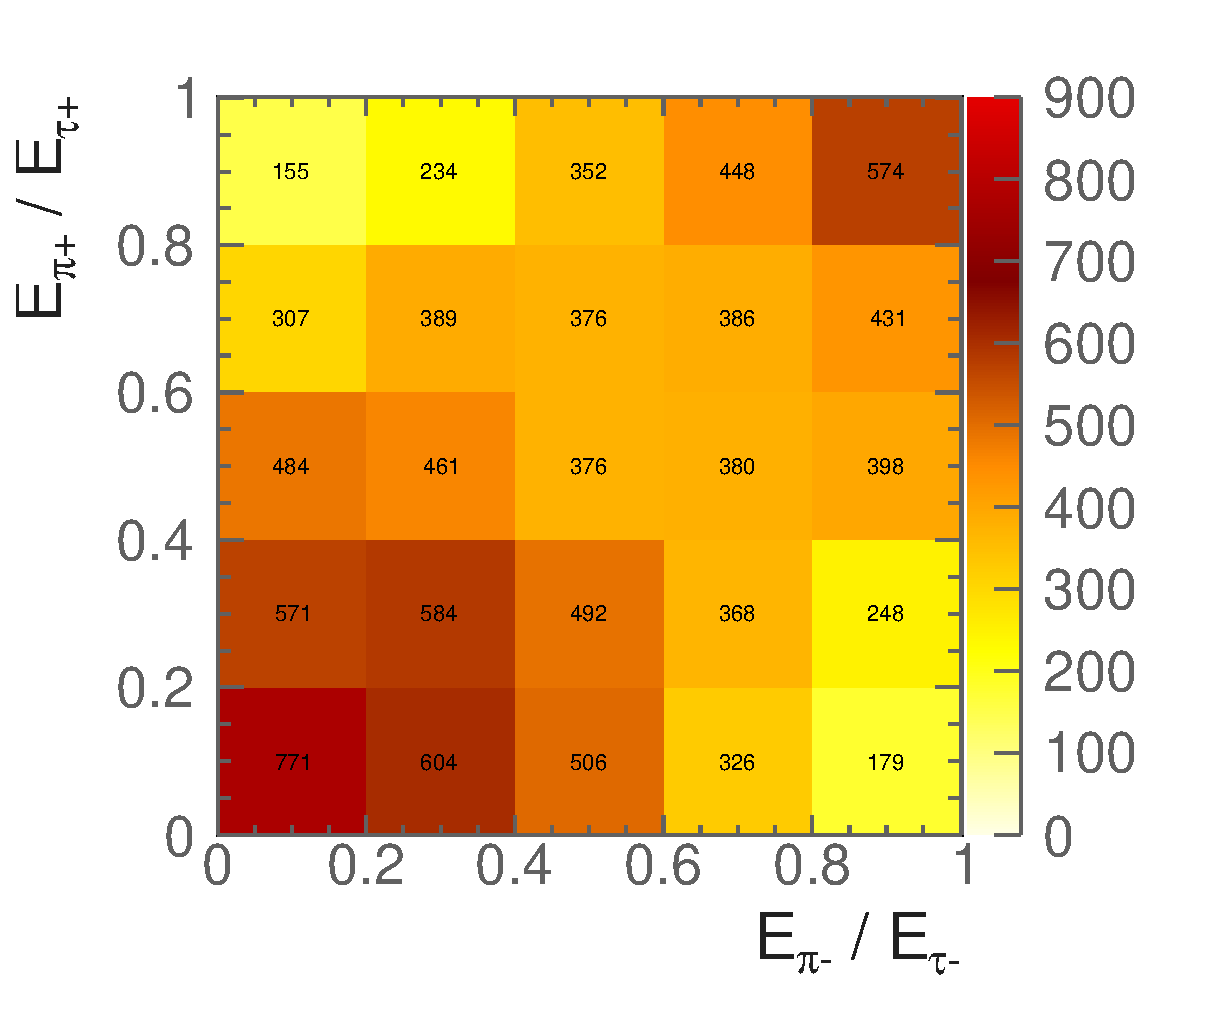
\includegraphics[width=\textwidth]{tau/NoTimeAnalysis/2DMC}
  \caption{Truth info.}
  \label{fig:TauSpin2DMC}
\end{subfigure}
\begin{subfigure}[b]{0.45\textwidth}
  \includegraphics[width=\textwidth]{tau/NoTimeAnalysis/2Dreco}
  \caption{Reconstructed}
  \label{fig:TauSpin2Dreco}
\end{subfigure}
\caption
{Two-dimensional plot of tau pair polarisation correlations from \PZ decay, using \tauToPion decay mode, for a) MC particles, and b) simulated and reconstructed particles.}
\label{fig:TauSpin2D}
\end{figure}
\begin{comment}
\begin{figure}[htbp]
\centering % \begin{center}/\end{center} takes some additional vertical space
\begin{subfigure}[b]{0.45\textwidth}
  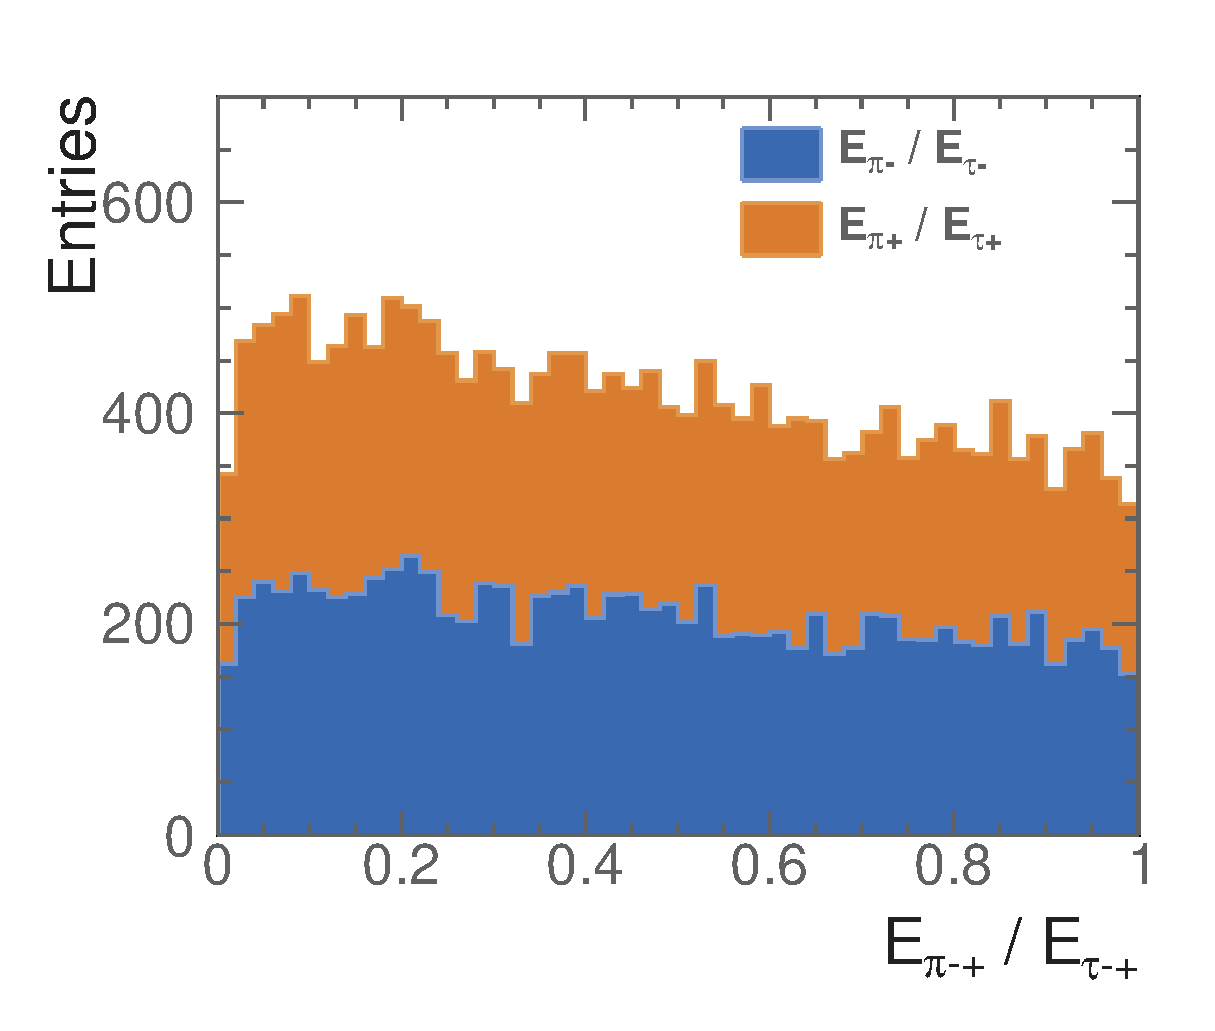
\includegraphics[width=\textwidth]{tau/NoTimeAnalysis/1DMC}
  \caption{Truth info.}
  \label{fig:TauSpin1DMC}
\end{subfigure}
\begin{subfigure}[b]{0.45\textwidth}
  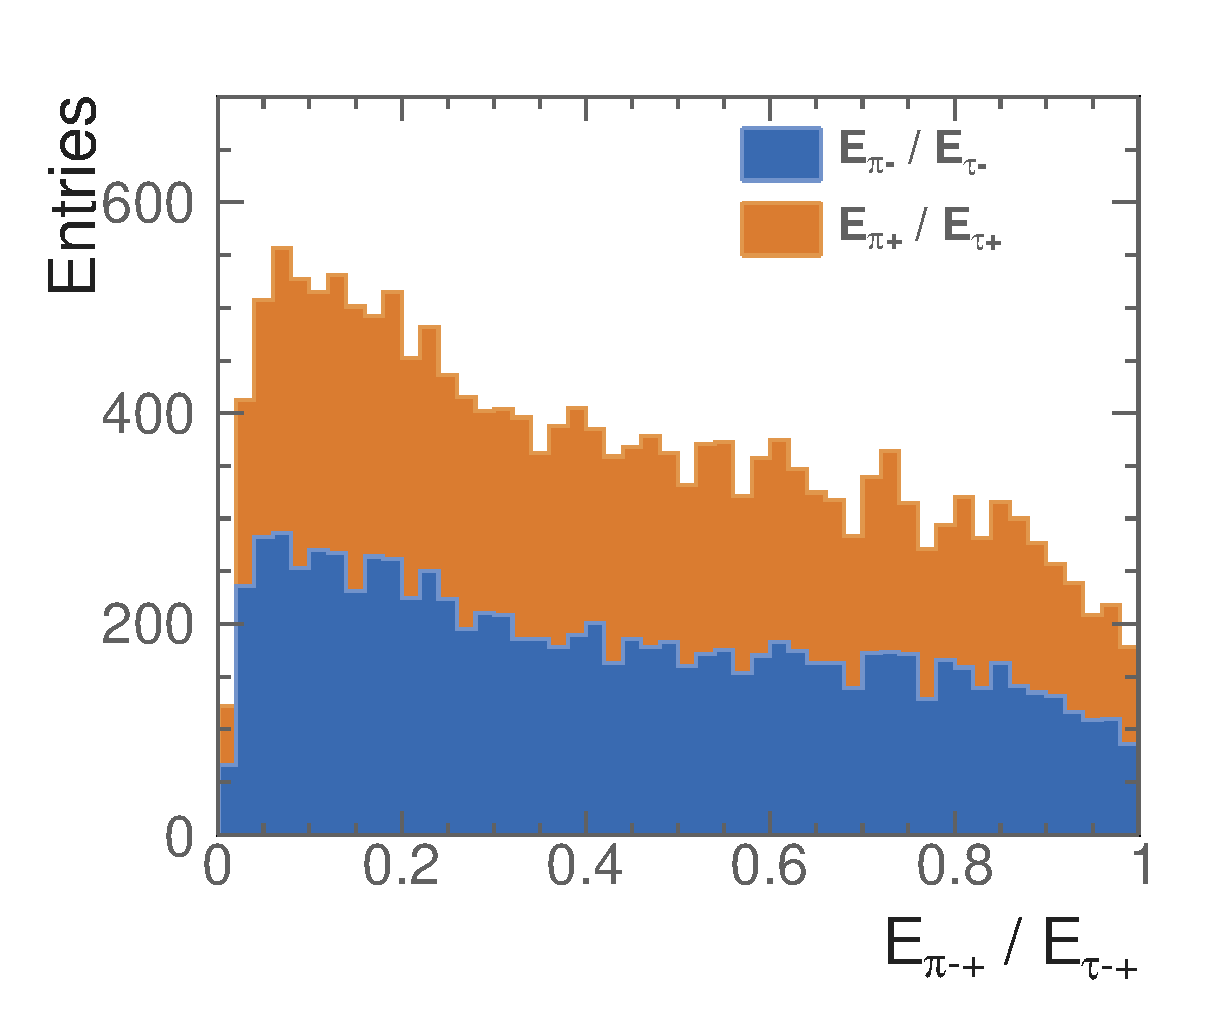
\includegraphics[width=\textwidth]{tau/NoTimeAnalysis/1DrecoNoOverflow}
  \caption{Reconstructed}
  \label{fig:TauSpin1Dreco}
\end{subfigure}
\caption[One-dimensional plot of spin correlations of the tau lepton pair from \PZ decay, using \decayPionShort decay mode.]
{One-dimensional plot of spin correlations of the tau lepton pair from \PZ decay, using \decayPionShort decay mode.}
\label{fig:TauSpin1D}
\end{figure}

\end{comment} 
  \chapter{Double Higgs Bosons Production Analysis}
\label{chap:DoubleHiggs}

\chapterquote{I believe it is impossible to be sure of anything.}%
{Han Fei Zi, 280 BC-233 BC}%: Blackwood's Magazine May 1830

Since the discovery of Higgs boson at the \LHC in 2012\cite{Aad:2012tfa,Chatrchyan:2012ufa}, it is crucial to understand the properties of the Higgs boson and test if it is a Standard Model Higgs. A number of theories beyond the Standard Model may be tested via the double Higgs production in an electro-positron collider (see \Section{sec:theoryHiggsBSM}). Generator level studies have shown that the precision reached by a multi-TeV linear collider, such as the Compact Linear Collider (\CLIC), is superior to that of the Large Hadron Collider (\LHC) and high luminosity upgraded \LHC  \cite{Contino:2013gna}.

%The Higgs mechanism and the Higgs boson in the Standard Model have been explained in \Chapter{chap:Theory}. even with 3000$fb^{-1}$ of data

The first challenge for the double Higgs bosons production analysis is the cross section(0.149\,fb at \rootS{1.4} and 0.588\,fb at \rootS{3}) is very small compared to background processes, making it difficult to select signal events. The second challenge is that at high centre-of-mass energies, events are boosted and many final-state particles are in the forward region of the detector, where the reconstruction performance is inferior to the barrel region and particles can escape detection.

In this chapter, a full \CLICILD detector simulation study has been performed for the double Higgs production, \eeToHH, via \WW fusion. Event generation and simulation will be discussed first. An overview of the analysis, including lepton finding and jet reconstruction, is presented, followed by an optimised multivariate analysis to distinguish signal from background processes. The optimised event selection is used to derive an estimate of the potential for the \CLIC. The results of this analysis have been publish in \Reference{Abramowicz:2016zbo}.
%The results of the signal selection are interpreted in the context of the Higgs self coupling.

\section{Analysis Straggly Overview}

Leading-order Feynman diagrams for double Higgs production via \WW fusion are shown in \Figure{fig:doubleHiggsFeynman}. The diagram shown in the \Figure{fig:doubleHiggsFeynman1} contains a triple Higgs vertex, which is sensitive to Higgs triple self coupling \gHHH. The diagram in the \Figure{fig:doubleHiggsFeynman2} is sensitive to quartic coupling \gWWHH. \FIGURE{fig:doubleHiggsFeynman3} and \Figure{fig:doubleHiggsFeynman4} show the Feynman diagrams of irreducible background processes for the study of \gHHH and \gWWHH.


\begin{figure}[!htbp]
  \begin{subfigure}[b]{0.22\textwidth}
    \includegraphics[width=\textwidth]{{{doubleHiggs/Feynman/1}}}
    \caption{}
    \label{fig:doubleHiggsFeynman1}
  \end{subfigure}
  \hfill
  \begin{subfigure}[b]{0.22\textwidth}
    \includegraphics[width=\textwidth]{{{doubleHiggs/Feynman/2}}}
    \caption{}
    \label{fig:doubleHiggsFeynman2}
  \end{subfigure}
  \begin{subfigure}[b]{0.22\textwidth}
    \includegraphics[width=\textwidth]{{{doubleHiggs/Feynman/3}}}
    \caption{}
    \label{fig:doubleHiggsFeynman3}
  \end{subfigure}
  \hfill
  \begin{subfigure}[b]{0.22\textwidth}
    \includegraphics[width=\textwidth]{{{doubleHiggs/Feynman/4}}}
    \caption{}
    \label{fig:doubleHiggsFeynman4}
  \end{subfigure}
\caption
   {The main Feynman diagrams for the leading-order \eeToHH processes at the \CLIC.}
   \label{fig:doubleHiggsFeynman}
\end{figure}

Double Higgs production can be also produced via {\HepProcess{ \Pep \Pem \to \PZ \PHiggs \PHiggs}\xspace}, where \PZ decays to \HepProcess{\Pnu \APnu}. This \HepProcess{\PZ \PHiggs \PHiggs} channel has also been used to study at future \ee colliders, for example, the \ILC at \rootSGeV{500} \cite{Baer:2013cma}. However, for the relevant \CLIC energies at \rootS{1.4} and 3\,TeV, its contribution to the \HepProcess{\PHiggs \PHiggs \Pnu \APnu} final state is small compared to that of the \WW fusion, and can be neglected at the centre-of-mass energies in this thesis.

%The cross section of {\HepProcess{ \Pem \Pep \to \PZ \PHiggs \PHiggs}\xspace} is one order of magnitude smaller than \eeToHH via the \WW fusion,  shown in \Figure{fig:theoryHiggsCrossSection},. Therefore, the effect of {\HepProcess{ \Pem \Pep \to \PZ \PHiggs \PHiggs}\xspace} present in \eeToHH channel at \rootS{1.4} and 3\,TeV is negligible.


%However, {\HepProcess{ \Pem \Pep \to \PZ \PHiggs \PHiggs}\xspace} can be easily identified via the recoil mass. Hence {\HepProcess{ \Pem \Pep \to \PZ \PHiggs \PHiggs}\xspace} is not considered in this studied.

From an experimental prospective, \eeToHH production has several distinct final-state topologies. In this chapter, \eeToHHbbWW sub-channel  is investigated. Firstly the hadronic decay mode of the \eeToHHbbWW channel is chosen to study because the hadronic decay has the largest cross section and does not produce primary neutrinos, which allows each \PW to be reconstructed. The semi-leptonic final state is also considered. However, the neutrinos produced at the final states make it  difficult to reconstruct the two Higgs bosons, as some momenta of one Higgs boson is missing. This channel is discussed briefly and its analysis strategy is adapted from the hadronic decay analysis.
%The double Higgs production, \eeToHH, is divided into two sub-channel: \eeToHHbbWW and \eeToHHbbbb to target the specific kinematic properties if each final state, which provides cross-validation between two sub-channels and an improvement in signal selection when combined.


%However, hadronic decay final state of the \eeToHHbbWW has a very low cross section. The signal selection is challenging and aggressive background rejection methods are deployed.
The analysis of the \eeToHHbbbb  sub-channel has been studied independently by collaborators. In this thesis, two analyses are combined for the final couplings extractions.
%The    is studied independently by collaborators. However, there is collaboration between the two studies. The two analyses are combined on the final couplings extractions.

%Combining with the low cross section, results for these two final states are not reported. The analysis can be easily (and have been) adapted for the semi-leptonic and leptonic final states.

The process, \eeToHHbbWWHadFull, results in a six quark final state with missing momentum. The high number of quarks requires an efficient jet reconstruction and a jet pairing algorithm to select the signal. The two \Pbottom quarks in the final states can be identified statistically with \Pbottom jet tagging. %Since the final state does not contain leptons, event-level lepton finding - typically for energetic isolated leptons -  would improve the signal selection efficiency.

A proof-of-principle generator-level study has already been performed using the \CLICILD detector model for \rootS{1.4} and 3\,TeV\cite{Linssen:2012hp}. In this chapter a full \CLICILD detector simulation study is presented. Firstly, suitable signal and background channels are identified. In order to select the signal, events with primary lepton identified are vetoed.  Vertex information is used to identify \Pbottom quark jets. \PFOs in an event are then clustered into jets depending on the number of quarks in the final states. Events selected based on this jet assignment are then used for pre-selection and multivariate analysis. This analysis is optimised independently for \rootS{1.4} and \rootS{3}.

% The \eeToHHbbWW hadronic decay will be presented first, followed by the semi-leptonic sub-channel analysis.




\section{Monte Carlo Sample Generation}


% TODO
% Understand beamsstrahlung and EPA
This section describes the Monte Carlo samples used in this simulation analysis. A full list of generated samples with their cross sections can be found in \Table{tab:doubleHiggsMCSamples}. Software used for sample generation is described in \Section{sec:pandoraMC}.


%Background samples considered in this analysis are listed in Table \ref{tab:doubleHiggsMCSamples}. The signal channel is \eeToHHbbWWFull where both \PW 's decay hadronically.
%W's decay hadronically? Does this make sense from a physics point of view?
%The analysis is performed with \CLICILD detector concept at \rootS{1.4} and 3\,TeV, and the semi-leptonic channel. Unless specified, the

Background processes with many quarks with missing momentum in the finial states would be challenging to reject, as the topologies are similar to that of the signal. Two example processes are \eeTo{ \Pquark \Pquark \Pquark \Pquark \Pnu \APnu} and \HepProcess{\Pepm\Pphoton \to \Pnu \Pquark \Pquark \Pquark \Pquark}. For the same reason, single Higgs boson production, such as \eeTo{\Pquark \Pquark \PHiggs \Pnu \APnu}, has a similar final state to the signal and it would also be difficult to reject. Therefore, a series of analysis tools are deployed to remove these background processes.

Some processes are not considered in this analysis because they either have very different event topologies, or they have very small cross sections. For example,  \HepProcess{\Egamma   \to \Pquark \Pquark \PHiggs \Plepton} is neglected  as the cross section is very small - even at \rootS{3}.

%For example, six-quark final states were not simulated due to constraints of the simulating software.
At high centre-of-mass energies, electron-photon and photon-photon interactions are important as their interactions become significant. These photons are produced due to the high electric field generated by the colliding beams. Processes involving real photons from beamsstrahlung (BS) and ``quasi-real'' photons are generated separately. For the ``quasi-real'' photon initiated processes, the Equivalent Photon Approximation (EPA) has been used \cite{lyth:jpa00215525}.

To separate Higgs production from other processes, all background processes are generated with a Higgs boson mass of 14\,TeV to ensure a negligible Higgs production. Processes involving Higgs production are simulated with a Higgs boson mass of 126\,GeV. The cross section of the signal, \eeToHHbbWW, is scaled according to \cite{Dittmaier:2012vm}.

%Multi-quark final state background samples could, in principle, contain higgs production. Therefore, they are generated with a Higgs mass of 14\,TeV. This will

% ATTN need to rewrite
The simulation and reconstruction chain is described in \Chapter{chap:Reconstruction}. For most background processes, events are generated requiring total invariant mass of quarks above 50\,GeV or 120\,GeV, because the invariant masses of the signal events are mostly above 150\,GeV.

%   For electron-photon interaction with $\Pquark\Pquark\Pquark\Pquark\Pnu$ final state at \rootS(1.4), events are simulated requiring invariant mass of quarks above 120\,GeV.

% These generator level cuts requires  limits are necessary to generate a large amount of background samples in a feasible timeframe, without losing significant signal samples.

Finally, the beam induced background \ggHad is simulated and overlayed on all samples. Details can be found in \Section{sec:pandoraggHad}.
% according to the integration time of each subdetector

\begin{table}[!tbp]\centering
% TODO fix lumi correction for e gamma, gamma e
% TODO change some of sample cross section for  electron-photon interaction with four quarks and a neutrino final state
\small
%{
\begin{tabular}{lr}
\hline \hline
Channel  &  $\sigma(\rootS{1.4})$ / fb   \\
\hline
\eeToHH & 0.149 \\
\hline
\eeToHHbbWWFull,hadronic & 0.018  \\
\eeToHHbbbbFull & 0.047 \\
\eeToHHotherFull & 0.085 \\
\hline
\eeTo{\qlight \qlight \PHiggs \Pnu \APnu}  & 0.86 \\
\eeTo{\Pcharm \APcharm \PHiggs \Pnu \APnu}  & 0.36 \\
\eeTo{\Pbottom \APbottom \PHiggs \Pnu \APnu}  & 0.31 \\

\eeTo{ \Pquark \Pquark \Pquark \Pquark}   &   1245.1\\
\eeTo{ \Pquark \Pquark \Pquark \Pquark \Plepton \Plepton}& 62.1* \\
\eeTo{ \Pquark \Pquark \Pquark \Pquark \Plepton \Pnu}& 110.4*\\
\eeTo{ \Pquark \Pquark \Pquark \Pquark \Pnu \APnu} & 23.2* \\

\eeTo{ \Pquark \Pquark} &  4009.5\\
\eeTo{ \Pquark \Pquark \Plepton \Pnu} &  4309.7\\
\eeTo{ \Pquark \Pquark \Pl \Pl} &  2725.8 \\
\eeTo{ \Pquark \Pquark \Pnu \Pnu} & 787.7  \\
\hline
\egamma{\Pepm}{\Pphoton}{BS}{\Pepm \Pquark \Pquark \Pquark \Pquark} & 2317  \\
%\egamma{\Pem}{\Pphoton}{BS}{\Pem \Pquark \Pquark \Pquark \Pquark} & 1160.7  \\
%\egamma{\Pep}{\Pphoton}{BS}{\Pep \Pquark \Pquark \Pquark \Pquark} & 1156.3 \\
\egamma{\Pepm}{\Pphoton}{EPA}{\Pepm \Pquark \Pquark \Pquark \Pquark} & 574 \\
%\egamma{\Pem}{\Pphoton}{EPA}{\Pem \Pquark \Pquark \Pquark \Pquark} & 287.1 \\
%\egamma{\Pep}{\Pphoton}{EPA}{\Pep \Pquark \Pquark \Pquark \Pquark}  & 286.9 \\
\egamma{\Pepm}{\Pphoton}{BS}{\Pnu \Pquark \Pquark \Pquark \Pquark}& 159.1\myDagger \\
%\egamma{\Pem}{\Pphoton}{BS}{\Pnu \Pquark \Pquark \Pquark \Pquark}& 79.8\myDagger \\
%\egamma{\Pep}{\Pphoton}{BS}{\APnu \Pquark \Pquark \Pquark \Pquark}& 79.3\myDagger \\
\egamma{\Pepm}{\Pphoton}{EPA}{\Pnu \Pquark \Pquark \Pquark \Pquark}& 34.7\myDagger  \\
%\egamma{\Pem}{\Pphoton}{EPA}{\Pnu \Pquark \Pquark \Pquark \Pquark}& 17.4\myDagger  \\
%\egamma{\Pep}{\Pphoton}{EPA}{\APnu \Pquark \Pquark \Pquark \Pquark}& 17.3\myDagger  \\
\egamma{\Pepm}{\Pphoton}{BS}{\Pquark \Pquark \PHiggs \Pnu} & 31.5* \\
%\egamma{\Pem}{\Pphoton}{BS}{\Pquark \Pquark \PHiggs \Pnu} & 15.8* \\
%\egamma{\Pep}{\Pphoton}{BS}{\Pquark \Pquark \PHiggs \Pnu} & 15.7* \\
\egamma{\Pepm}{\Pphoton}{EPA}{\Pquark \Pquark \PHiggs \Pnu} & 6.78* \\
%\egamma{\Pem}{\Pphoton}{EPA}{\Pquark \Pquark \PHiggs \Pnu} & 3.39* \\
%\egamma{\Pep}{\Pphoton}{EPA}{\Pquark \Pquark \PHiggs \Pnu} & 3.39*   \\
\hline
\gammagamma{\Pphoton}{BS}{\Pphoton}{BS}{ \Pquark \Pquark \Pquark \Pquark}& 21406.2*  \\
\gammagamma{\Pphoton}{BS}{\Pphoton}{EPA}{ \Pquark \Pquark \Pquark \Pquark}& 4018.7* \\
\gammagamma{\Pphoton}{EPA}{\Pphoton}{BS}{ \Pquark \Pquark \Pquark \Pquark}& 4034.8* \\
\gammagamma{\Pphoton}{EPA}{\Pphoton}{EPA}{ \Pquark \Pquark \Pquark \Pquark}& 753.0* \\
\hline \hline
\end{tabular}

\caption[Signal and background samples with the corresponding cross sections at \rootS{1.4}.]{List of signal and background samples with the corresponding cross sections at \rootS{1.4}. \Pquark can br \Pup, \Pdown, \Pstrange, \Pbottom or \Ptop. Unless specified, \Pquark, \Plepton and \Pnu represent particles and its corresponding anti-particles. \Pphoton(BS) represents a real photon from beamstrahlung (BS). \Pphoton(EPA) represents a ``quasi-real'' photon, simulated with the Equivalent Photon Approximation. For processes labeled with * and $\myDagger$, the generator-level cut requires invariant mass of quarks greater than 50 and 120\,GeV, respectively.}
\label{tab:doubleHiggsMCSamples}
\end{table}
%Simulated \PW has invariant mass of 80.385\,GeV.

\section{Lepton identification}
\label{sec:doubleHiggsLepton}

The event reconstruction was performed using the Marlin framework and reconstruction package in \ilcsoft v01-16. Separate software packages (processors) were optimised for lepton identification and for jet reconstruction. %New processors have been developed and existing processors have been optimised for signal selection and background rejection.
%The reconstruction is done via Marlin in \ilcsoft v01-16. The latest functioning flavour tagging processor exist in \ilcsoft v01-16. Thus newer versions of  \ilcsoft can not be used in this analysis.


For the signal channel, \eeToHHbbWWHad, there is no primary lepton in the final state, whilst many background  processes, such as \HepProcess{\Pquark \Pquark \Pquark \Pquark \Plepton \Pnu}, contain primary leptons in final states. Hence, effectively rejecting events with primary leptons is an important step in the event selection. Primary leptons deposit energies in the tracking calorimeter. The start of the energy deposition is typically within 0.05\,mm to the interaction point. These primary leptons are also typically energetic and often isolated from other particles. Whilst electrons and muons are stable enough to deposit energies in calorimeters, tau leptons are very short lived. With a typical decay length of 87\,$\mu{m}$, it decays before reaching vertex detector. Therefore, only decay products of the tau leptons can be reconstructed.

\subsection{Electron and muon identification}
\label{sec:doubleHiggsLeptonID}

Two Marlin reconstruction for processors for light lepton(\Pe, \Pmu) tagging are used and optimised. As it is important to identify primary light leptons to help to select signal events, two additional light lepton tagging processors are developed and optimised.

 %described followed by their performances. As the signal is very rare comparing to the background, it is necessary to develop high performance isolated lepton finder to veto events with leptons and improve the signal selection efficiency. An existing lepton finder is optimised in \Section{sec:doubleHiggsIsolatedLeptonFinder} and a separate lepton finder is developed by the author in \Section{sec:doubleHiggsBonoLeptonFinder}.

\subsubsection{\IsolatedLeptonFinderProcessor}
\label{sec:doubleHiggsIsolatedLeptonFinder}
\IsolatedLeptonFinderProcessor reconstruction package is used, modified, and optimised. This processor identifies high energy electrons and muons that are isolated from other particles. Optimal parameters are chosen and tested using the signal channel and the \eeTo{ \Pquark \Pquark \Pquark \Pquark \Plepton \Pnu} channel, which is multi quark final state with a primary lepton.

Electron induced electromagnetic showers are mostly contained in the \ECAL. The primary electrons and muons from the electron-positron interaction leaves primary tracks in the tracking detector, which start typically less than 0.05\,mm from the interaction point. The isolation criteria requires the lepton to be spatially separated from other high energy particles.

Optimal values of the processor are listed in \Table{tab:doubleHiggsIsolatedLeptonFinder}. $E$ is the energy of the lepton. $E_{\ECAL}$ is the energy of the lepton deposited in the \ECAL. $E_{cone}$ is the total energy within a cone of an opening angle of $\cos^{-1}(0.995)$ around the lepton. $d_0$, $z_0$, and $r_0$ are the Euclidean distance of the lepton track starting point to the interaction point in x-y plane, in z direction, and in x-y-z three dimensional space, respectively. Performance of the processor is shown in \Table{tab:doubleHiggsIsoLepPerformance}.

\begin{table}[!htbp]
\begin{tabular}{lr}
\hline
\hline
\IsolatedLeptonFinderProcessor  & Selection \\
\hline
High Energy (GeV) &  $E > 15$  \\
\Pepm ID & $\frac{E_{\ECAL}}{E} > 0.9$ \\
\Pmupm ID &  $ 0.25> \frac{E_{ECAL}}{E} > 0.05$\\
Primary Track (mm) & $d_0 < 0.02, z_0 < 0.03, r_0 < 0.04$ \\
Isolation (GeV)& $E_{cone}^2 \leqslant 5.7 \times E - 50$ \\
\hline
\hline

\end{tabular}
\caption
{Optimised parameters of \IsolatedLeptonFinderProcessor}
\label{tab:doubleHiggsIsolatedLeptonFinder}
\end{table}

\subsubsection{\BonoLeptonFinder}
\label{sec:doubleHiggsBonoLeptonFinder}

A complimentary light lepton finder, \BonoLeptonFinder is developed to further identify energetic isolated light leptons. Comparing to the \IsolatedLeptonFinderProcessor, the main difference is that the \BonoLeptonFinder utilises particle ID information provided by \pandora to identify leptons.

%\IsolatedLeptonFinderProcessor has strict criterion to find high-energy isolated leptons to avoid mistakes. However, since the signal cross section is low in this analysis, it would be beneficial to reject more events with leptons identified to improve the signal to background ratio. Hence another isolated lepton finder is developed. The main feature of the \BonoLeptonFinder is that it utilises calorimetric information provided by \pandora.


The processor uses two sets of cuts to identify energetic isolated light leptons. If a lepton passes either set of cuts, it will be identified by the processor. The first set of cuts uses the particle ID information from \pandora, demanding a \pandora electron or muon with high \pT and a primary track. The identified lepton should either have a very high transverse momentum or be isolated. The second set of cuts uses \ECAL energy fraction to determine the light lepton ID. The rest of the cuts are very similar to the first cuts. The second cuts contain stricter isolation criterion to reduce fake rate.
%Not sure the last sentence above makes sense

\begin{table}[!htbp]
\begin{tabular}{lr}
\hline
\hline
\BonoLeptonFinder  & Selection \\
\hline
High Energy (GeV) &  $E > 10$  \\
\Pepm ID & \pandora reconstructed \& $\frac{E_{\ECAL}}{E} > 0.95$ \\
\Pmupm ID &  \pandora reconstructed\\
Primary Track (mm) & $r_0 < 0.015$ \\
a) High Transverse Momentum (GeV) &  $\pT > 40$  \\
b) Isolation (GeV)& $E \geqslant 23 \times \sqrt{E_{cone1}} + 5$ \\
\hline
High Energy (GeV) &  $E > 10$  \\
\Pepm ID & $\frac{E_{\ECAL}}{E} > 0.95$ \\
\Pmupm ID & $0.2 > \frac{E_{\ECAL}}{E} > 0.05$ \\
Primary Track (mm) & $r_0 < 0.5$ \\
a) High Transverse Momentum (GeV) &  $\pT > 40$  \\
b) Isolation (GeV)& $ E \geqslant 28 \times \sqrt{E_{cone2}} + 30$ \\
\hline
\hline

\end{tabular}
\caption[Optimised parameters  of \BonoLeptonFinder.]
{Optimised parameters  of \BonoLeptonFinder. A lepton needs to pass either sets of cuts to be identified. Within a set, the lepton needs to satisfy either condition a) or b).}
\label{tab:doubleHiggsBonoLeptonFinder}
\end{table}

\TABLE{tab:doubleHiggsBonoLeptonFinder} lists the  selection cuts for \BonoLeptonFinder. Variables are defined same to those for \IsolatedLeptonFinderProcessor. \pT is the transverse momentum. $E_{cone1}$ and $E_{cone2}$ are the total energy of PFOs within a cone of an opening angle of $\cos^{-1}(0.995)$ and $\cos^{-1}(0.99)$ respectively around the lepton. The performance of the processor is shown in \Table{tab:doubleHiggsIsoLepPerformance}.


\subsubsection{Comparison: \IsolatedLeptonFinderProcessor versus \BonoLeptonFinder}

The two processors share similar criterion for light lepton identification. The main difference is that the \BonoLeptonFinder uses particle identification from \pandora, which takes into account extra calorimetric information to determine the particle ID than simple \ECAL energy fraction. \BonoLeptonFinder also allows high \pT light leptons to be identified in a non-isolated environment.
%aggressive nature of the \BonoLeptonFinder. %The performance of two processors on the signal and selected background samples is shown in \Table{tab:doubleHiggsIsoLepPerformance}.

\subsection{Tau lepton identification}

Tau leptons have a short life-time. With a typical decay length of 87\,$\mu{m}$, tau lepton decays before reaching the vertex detector and can only be identified through the reconstruction of their decay products. The leptonic decay of tau lepton can be identified using the isolated lepton finder processors described above. Therefore in this section, tau identification will focus on the tau lepton hadronic decay.

\TauFinderProcessor reconstruction package is optimised. In addition, \BonoTauFinder is developed to provide additional tau lepton identification.

%To improve signal selection, a tau lepton identifier is developed by the author in \Section{sec:doubleHiggsBonoTauFinder}.



\subsubsection{\TauFinderProcessor}

% TODO check tau stuff

\TauFinderProcessor \cite{LCD-Note-2010-009} reconstruction package has been optimised.

Tau finder forms a tau search cone, containing tau lepton decay products, using a cone clustering algorithm (see  \Section{sec:pandoraConeCluster}). A high energy track is selected as a seed and a small cone is formed around it. The \PFOs inside the cone are required to be consistent with a tau hadronic decay: no more than 3 charged particles, invariant mass close to tau mass and few \PFOs in the cone. The cone is required to be isolated from other particles. To reduce fake rate, low momentum and very forward particles do not participate in the tau finding, as they more likely come from \ggHad background.


The optimised parameters are listed in \Table{tab:doubleHiggsTauFinderProcessor}. Variables are defined in the same way as in previous sections. $\theta_Z$ is the polar angle w.r.t. the beam axis. $N_{X^+}$ and $N_{tau}$ are the number of charged particles and the number of \PFOs respectively in the tau cone. $m_{tau}$ is the invariant mass of the sum of the PFOs in the tau candidate. $E_{cone}$ is the total energy of \PFOs within a cone of an opening angle between 0.03 and 0.33\,rad  around the tau seed. The performance of the processor is shown in \Table{tab:doubleHiggsIsoLepPerformance}.

\begin{table}[!htbp]
\begin{tabular}{lr}
\hline
\hline
\TauFinderProcessor  & Selection \\
\hline
Veto \ggHad (GeV) &  $\pT < 1$, $\absOf{\cos\left(\theta_Z\right)} > 1.1$  \\
Seed particle (GeV) & $\pT > 10$ \\
Tau candidate cone opening angle (rad) & 0.03 \\
Tau candidate rejection & $N_{X^+} > 3$, $N_{tau} > 10$, $m_{tau} > 2$   \\
Isolation (GeV)&  $ E_{cone} < 3$\\
\hline
\hline
\end{tabular}
\caption
{Optimised parameters of \TauFinderProcessor.}
\label{tab:doubleHiggsTauFinderProcessor}
\end{table}

\subsubsection{\BonoTauFinder}
\label{sec:doubleHiggsBonoTauFinder}

\BonoTauFinder, developed by the author, identifies high momentum particles as tau seeds. Particles are iteratively added to the search cone in the order of the ascending opening angle to the seed. After each particle addition, the temporary search cone is then considered as a temporary  tau candidate and tested for isolation and consistency  with tau hadronic decay signature. The temporary tau candidate only needs to pass one of the isolation conditions to be identified as a tau candidate. The iterative particle addition procedure stops when the cone opening angle is larger than a threshold. If multiple temporary tau candidates of the same tau seed pass the selection, the one with smallest opening angle is chosen to form the final tau candidate. To reduce fake tau decay products from \ggHad background, low energy particles do not participate.

This tau finder has different isolation criterion for tau 1-prong decay and 3-prong decay, reflecting different topologies of different tau decay final states.

%tau hypothesis singular or tau hypotheses plural?


\TABLE{tab:doubleHiggsTauFinderProcessor} lists the optimised parameters  for \BonoTauFinder. Variables are defined in the same wasy as those in previous sections. $\theta_S$ is the opening angle of the search cone. $cone1$ and $cone2$ are defined as a cone of an opening angle of $\cos^{-1}(0.95)$, and $\cos^{-1}(0.99)$ respectively around the tau seed. $r_0$ is referring to tau seed particle. The performance of the processor is shown in \Table{tab:doubleHiggsIsoLepPerformance}.

\begin{table}[!htbp]
\begin{tabular}{lr}
\hline
\hline
\BonoTauFinder  & Selection \\
\hline
Veto \ggHad (GeV) &  $E < 1$\\
Seed particle (GeV) & $\pT > 5$ \\
Maximum search cone opening angle (rad) & $\theta_S \leqslant \cos^{-1}(0.999)$\\
Tau candidate rejection & $N_{X^+} \neq 1,3$, $m_{PFO} > 3$   \\
Isolation (GeV) 1& $N_{cone1} = 0$, $ \pT_{cone} \geqslant 10$\\
Isolation (GeV) 2& $N_{X^+} = 1$, $N_{cone1} = 1$, $r_0 > 0.01$\\
Isolation (GeV) 3& \multicolumn{1}{R{0.4\textwidth}}{{$N_{X^+} = 3$, $N_{cone1} = 1$, $ \pT_{cone} \geqslant 10$, $\theta_S < \cos^{-1}(0.9995)$}}\\
Isolation (GeV) 4& \multicolumn{1}{R{0.4\textwidth}}{$N_{X^+} = 1$, $N_{cone2} = 0$, $r_0 > 0.01$, $ \pT_{cone} \geqslant 10$}\\
Isolation (GeV) 5& \multicolumn{1}{R{0.4\textwidth}}{{$N_{X^+} = 3$, $N_{cone2} = 0$, $ \pT_{cone} \geqslant 10$, $\theta_S < \cos^{-1}(0.9995)$}}\\
\hline
\hline

\end{tabular}
\caption
{Optimised parameters of \BonoTauFinder}
\label{tab:doubleHiggsBonoTauFinderProcessor}
\end{table}


\subsubsection{Comparison: \TauFinderProcessor v.s. \BonoTauFinder}

The main difference is that the \BonoTauFinder has an iterative approach to build up a tau candidate, which allows a dynamic tau search cone size. The \BonoTauFinder also has smaller cut values on minimum \pT and invariant mass, but stricter isolation criterions. The performances of processors are shown in \Table{tab:doubleHiggsIsoLepPerformance}.
%I've reworded the first sentence in this para - does it make sense?
%looser cut - is this the accepted term? if not, maybe replaced the word looser with something else

\subsection{Very forward electron identification}
\label{sec:doubleHiggsForwardElectron}

At high \sqrtS, particles are boosted and it is important to extract information in the forward calorimeters to aid signal selection. Certain background channels, for example photon-electron interactions, can have energetic primary  electrons in  the forward calorimeters, the \LumiCAL and the \BeamCAL. The signal selection will benefit if these primary electrons in the forward calorimeters are identified.

It is challenging to identify electrons in these forward calorimeters. As forward calorimeters have very low angular acceptances, most particles in these forward detector would be very forward particles from beam induced background. However,  \cite{sailer2012radiation} shows that sufficiently high energy electrons can be efficiently identified in the \BeamCAL and \LumiCAL.

For the \CLICILD detector concept, energies deposited in the \LumiCAL and the \BeamCAL are not reconstructed in simulation. This is because the thousands of beam induced background particles per bunch crossing requires expensive computational resources. However, previous studies \cite{Sailer:2017onh,Lukic:forwardElectron} using parameterise the particle ID efficiency using MC particles give equivalent performance to the full detector simulation approach.


%The current simulation software could not handle the simulation in a feasible time. Therefore, the adopted approach is to parameterise the background particle energy deposition leading to electron tagging algorithms.
%I changed 'and leads to' to 'leading to'. Is that what you meant? The original text was mixing tenses

For the \BeamCAL, \cite{Sailer:2017onh} describes an electron tagging algorithm developed using \rootS{3} collision environment by comparing the simulated electron and background energy distributions. An electron is tagged if the energy is significantly larger than the expected background energy distributions. Events are overlaid with background energy deposition integrated over 40 bunch crossing. The tagging efficiency for electrons with energy 500 to 1500\,GeV are binned in histograms at an interval of 100\,GeV. There is no tagging for electrons with energy below 500\,GeV or about 1500\,GeV. In addition, this efficacy tagging approach  most likely underestimates efficiencies due to the coarse binning of energies. I.e. a 650\,GeV particle is treated the same as a 600\,GeV particle. An indicative performance plot of 500\,GeV electron tagging efficiency as a function of polar angle is shown in \Figure{fig:doubleHiggsForwardBCAL}.

%A C++ code library has been developed and used in this analysis.

The input of the \BeamCAL electron tagging algorithm is the four momenta of the MC electron. Since the algorithm assumes collisions at \rootS{3}, for the \rootS{1.4} user case, the momenta of the MC electron is scaled down by a factor of $\frac{3}{1.4}$.

\begin{figure}[!tbp]
  \begin{subfigure}[b]{0.45\textwidth}
    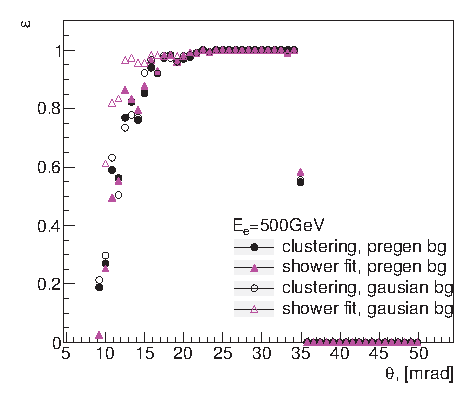
\includegraphics[width=\textwidth]{{{doubleHiggs/forward/ForwardBCAL}}}
    \caption{}
    \label{fig:doubleHiggsForwardBCAL}
  \end{subfigure}
  \hfill
  \begin{subfigure}[b]{0.45\textwidth}
    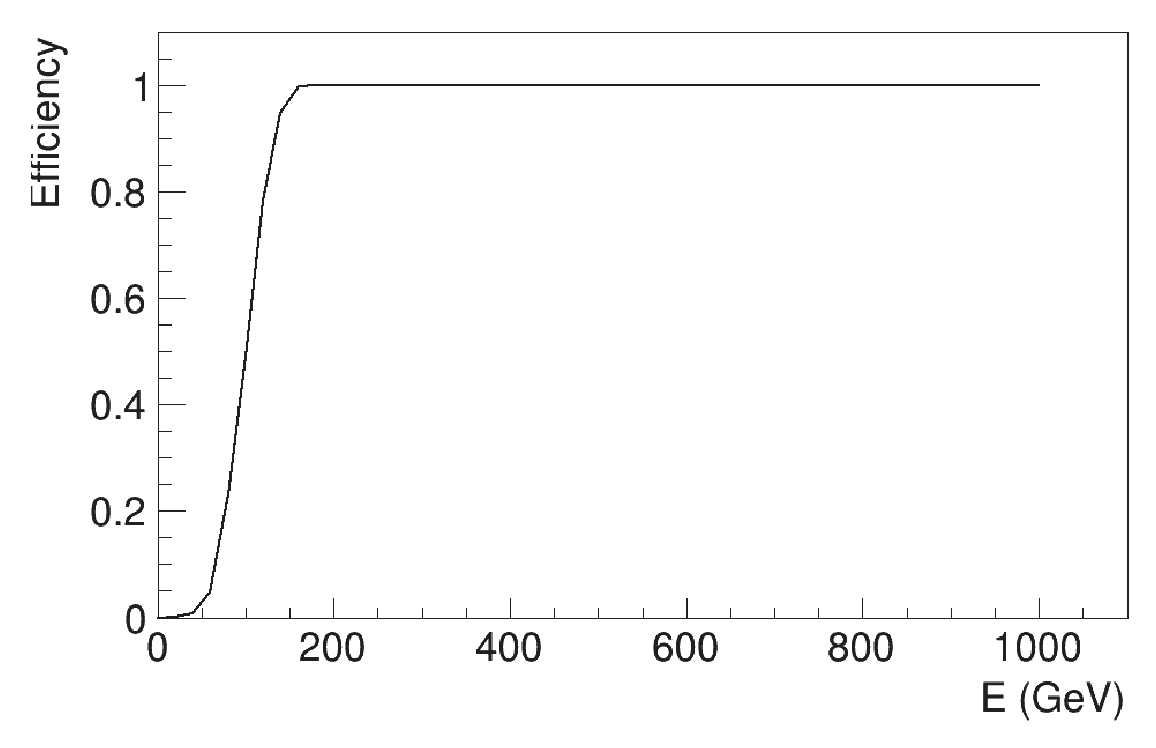
\includegraphics[width=\textwidth]{{{doubleHiggs/forward/ForwardLCAL}}}
    \caption{}
    \label{fig:doubleHiggsForwardLCAL}
  \end{subfigure}
\caption[\BeamCAL and \LumiCAL electron tagging efficiency.]%
   {\FIGURE{fig:doubleHiggsForwardBCAL} shows \BeamCAL 500\,GeV electron tagging efficiency as a function of polar angle with different methods to model backgrounds and fittings, taken from \cite{Sailer:2017onh}. \FIGURE{fig:doubleHiggsForwardLCAL} shows the \LumiCAL  electron tagging efficiency as a function of the electron energy, for polar angle $\theta = 50\,mrad$, taken from \cite{Lukic:forwardElectron}. }
   \label{fig:doubleHiggsForwardCAL}
\end{figure}

For the \LumiCAL,  \Figure{fig:doubleHiggsForwardCAL} shows the \LumiCAL  electron tagging efficiency as a function of the electron energy for polar angle $\theta = 50\,mrad$ where events are overlaid with background energy deposition integrated over 100 bunch crossings. Assuming that the \LumiCAL electron tagging efficiency in this analysis is the same as in \Figure{fig:doubleHiggsForwardCAL} for all polar angles and for \rootS{1.4} and 3\,TeV, \LumiCAL electron tagging efficiency, $\varepsilon$, is parameterised as

%The \LumiCAL electron tagging in this analysis is based on the performance plot in \Figure{fig:doubleHiggsForwardCAL}.

%the \HepProcess{\PHiggs \to \Pmu \Pmu} analysis in \cite{Milutinovic-Dumbelovic:2014uta,Grefe:2012rt} has developed an algorithm for electron tagging in the \LumiCAL with similar logic to the algorithm for the \BeamCAL.
% as this is the only study available for comparison.


\begin{equation}
\varepsilon=
\begin{cases}
  0, & \text{if}\ E < 50\,GeV,\\
  0.99 \times \frac{(erf(E - 100) + 1 )}{2}, & \text{otherwise},
\end{cases}
\end{equation}
where $E$ is the energy of the electron or the photon and $erf$ is the error function. For each MC electron in the \LumiCAL a random number between 0 and 1 is generated. If the random number is less than \varepsilon the MC electron is tagged.

%(see \Table{tab:detectorForwardILDvsCLICILD} for detector coverage)
Due to lack of tracking ability in the forward region, electrons and photons can not be differentiated in forward calorimeters. Therefore, both photons and electrons are tagged by the above algorithms.

%appear indistinguishable to the \BeamCAL and \LumiCAL and both photons and electrons are tagged by the above algorithms.


 %Due to the lack of tracking in these region, electrons and photons would have the same electromagnetic shower profile, with the given calorimeter resolution. MC photons and electrons are checked if they fall in the LCal or the BCal, and checked against the known detection efficiency.


%With the increase of the centre-of-mass energy, more  As discussed before, veto events with leptons help the signal selection. Hence the goal is to identify leptons in the forward region.

%These forward calorimeters were not simulated due to computational limitation.
% For \rootS(3), the BeamCal detection efficiency is provided by a software package \cite{}. For \rootS(1.4), the same software for the BeamCal is used, by scaling the energy of the MC particle by a factor of $\frac{3}{1.4}$. For the LumiCal, the identification efficiency is defined as


\subsection{Lepton identification performance}

The performance of all lepton finding processors on the signal and selected background process is shown in \Table{tab:doubleHiggsIsoLepPerformance}. The percentages represent the events without identified primary leptons.  \BonoLeptonFinder and \BonoTauFinder reject more background events than the \IsolatedLeptonFinderProcessor and \TauFinderProcessor. By combining the processors, 86.6\% signal events remain and 16.8\% of \HepProcess{\Pep \Pem \to \Pquark\Pquark\Pquark\Pquark\Plepton\Pnu} events survive after rejecting events where leptons are identified.
%Second sentence: can you say "" becase this would read better

\begin{table}[!tbp]
\begin{tabular}{lrr}
\hline
\hline
Efficiency (1.4\,TeV)  &  Signal & \HepProcess{\Pep \Pem \to \Pquark\Pquark\Pquark\Pquark\Plepton\Pnu} \\
\hline
\IsolatedLeptonFinderProcessor & 99.3\% & 50.3\%  \\
\BonoLeptonFinder & 99.1\% & 39.9\%  \\
\TauFinderProcessor & 97.5\% & 52.3\%  \\
\BonoTauFinder & 89.7\% & 38.5\%  \\
Forward Finder Processors & 98.9\% & 95.1\%  \\
\hline
Combined & 86.6\% & 16.8\%  \\
\hline
\hline

\end{tabular}
\caption{Isolated lepton finder processors performance on the signal and selected background events at \rootS{1.4}.}
\label{tab:doubleHiggsIsoLepPerformance}
\end{table}


The forward lepton finders are most effective at rejecting background events with primary leptons in the forward region. \TABLE{tab:doubleHiggsForwardPerformance} shows the performance of the processors with the signal and the  \egamma{\Pem}{\Pphoton}{BS}{\Pem \Pquark \Pquark \Pquark \Pquark} background events. 53.6\% of \egamma{\Pem}{\Pphoton}{BS}{\Pem \Pquark \Pquark \Pquark \Pquark} background events survive after rejecting events with primary leptons identified.


\begin{table}[!tbp]
\begin{tabular}{lrr}
\hline
\hline
Selection / Efficiency (1.4\,TeV)  &  Signal & \egamma{\Pem}{\Pphoton}{BS}{\Pem \Pquark \Pquark \Pquark \Pquark}  \\
\hline
Combined light lepton finder & 87.6\% & 67.5\%  \\
Forward Finder Processors & 98.9\% & 53.6\%  \\
\hline
Combined & 86.6\% & 30.8\%  \\
\hline
\hline

\end{tabular}
\caption{Very forward electron and photon finder performance on the signal and selected background events at \rootS{1.4}.}
\label{tab:doubleHiggsForwardPerformance}
\end{table}


\subsection{Other lepton identification processors}


Other isolated lepton identification processors have been tested, including IsolatedLeptonTagging and TauJetClustering. They either performed poorly comparing to the processors above, or became redundant after using the processors above. Therefore, these lepton identification processors are not used in this analysis.
%ATTN: does calibration/optimisation work better than tuning parameters?

\section{Jet reconstruction}

For the signal channel, \eeToHHbbWWHad, one Higgs boson decays to two \Pbottom quarks, resulting in two jets from quark hadronisation. Similarly the other Higgs boson decays to two \PW bosons, where each \PW boson decays into two quarks. Therefore, the expected number of jets is six.  Physical bosons,  \PW and \PHiggs, can be reconstructed from jets. Therefore, it is important to have efficient jet reconstruction to reconstruct physical bosons and the signal events. In this section, the optimisation of the jet reconstruction is discussed.

% A useful technique for the analysis is to reconstruct the multi-jet final state using jet algorithms. This allows discriminative variables to be calculated. A brief discussion about jet algorithms and its relevance for the \CLIC and this analysis are provided.

\subsection{Jet reconstruction optimisation}
\label{sec:doubleHiggsJetOptimisation}
Jet reconstruction algorithms group particles into jets. An overview of the jet algorithms can be found in \Section{sec:pandoraJetAlg}. Longitudinal invariant, \kt, jet algorithm is chosen for the jet clustering. The free parameters for \kt algorithm are the $R$ parameter, which controls the radius of the jet, and the choice of the \PFO collection, which incorporates different level of timing and \pT cuts to reduce beam induce background (see \Section{sec:pandoraggHad}).
%Both parameters are optimised for \rootS{1.4} and \rootS{3}.

The metric for optimising the $R$ parameter, and the \PFO collection, is the invariant mass and mass resolution of \PHiggs and \PW. An optimised jet reconstruction is chosen such that invariant masses of \PHiggs and \PW are close to their true masses, and invariant mass widths are small.

%For the jet reconstruction optimisation, only signal events are used and jets are paired to using MC truth information (see \Section{sec:pandoraMCtruthLink}).

%The sample for the optimisation is \eeToHH.

The signal channel, hadronic decay of \eeToHHbbWWHad, is used for the jet reconstruction optimisation. The signal events  are processed through \kt jet algorithm  in the 6-jet exclusive mode. The six jet are paired using the MC truth information (see \Section{sec:pandoraMCtruthLink}) by examining the decay chain of MC particles. Four invariant mass distributions are obtained: two Higgs masses, $m_{\Hbb}$, $m_{\HWW}$, and two \PW masses $m_{\PW}$, $m_{\W*}$. \W* indicates the off-mass-shell \PW boson because when a Higgs boson decays into two \PW bosons, one \PW is off the mass shell, as the Higgs mass is less than the sum two \PW masses (see \Section{sec:theoryHiggsBoson}).
%The six jets are paired up using  MC truth information to the corresponding Higgs and \PW boson.
%I'm not sure this last sentence is worded correctly. Doesn't make sense to me but I'm not a physicist!

\paragraph{Mass resolution fit}
Three invariant mass distributions are compared for optimising jet reconstruction:  $m_{\Hbb}$, $m_{\HWW}$, and $m_{\PW}$. The optimal jet reconstruction should produce a sharp mass peak around the particle's simulated mass (see \Section{sec:pandoraCLICsimMass}). An example of $m_{\Hbb}$ invariant mass distribution is shown in \Figure{fig:doubleHiggsFitMCMass}. An analytical functional form is fitted to quantitatively describe the shape. The basic fitting function is a Gaussian function. Although the underlying mass distribution of particles like $m_{\PW}$ is a Breit-Wigner distribution, the overall mass distribution is Gaussian like, as the overall mass distribution is a convolution of a narrow \PW Breit-Wigner distribution and a wide Gaussian distribution for the detector resolution. The $m_{\Hbb}$  mass distribution is gaussian like but with asymmetrical width, due to \Pbottom quarks decaying to neutrinos, leading to a loss of detectable particles.

As only the peak region of the mass distribution is Gaussian like, free parameters are used in the fitting function to fit the tail distribution. The fitting function takes the form of
\begin{equation}
f(m)=A e^{- \frac{(m - \mu)^2}{g}}
\end{equation}
\begin{equation}
g=
\begin{cases}
2\sigma_L + \alpha_L(m - \mu), & \text{if}\ m < \mu,\\
2\sigma_R + \alpha_R(m - \mu), & \text{if}\ m \geqslant \mu,
\end{cases}
\end{equation}
where $m$ is binned mass distribution with 50 bins in range [0, 200]\,GeV. $\mu$ is the fitted mass peak position in GeV. $\sigma_L$ and $\sigma_R$ allow asymmetrical width of the distribution. $\alpha_L$ and  $\alpha_R$  control the fit of tail distribution.  $A$ is the normalisation factor.


\begin{figure}[!htbp]
\includegraphics[width=\largefigwidth]{doubleHiggs/MCmassFit}
\caption[Example MC mass fit for jet optimisation in double Higgs analysis]%
   {A typical example of  $m_{\Hbb}$  mass distribution with the superimposed fitting function in red. The arrow shows the fitted mean peak position in GeV.}
   \label{fig:doubleHiggsFitMCMass}
\end{figure}

\paragraph{Optimal $R$ and \PFO collection}

%The mass fit is performed for $m_{\Hbb}$, $m_{\HWW}$, and $m_{\PW}$ distributions.  The optimal jet reconstruction should have the mass peak close to the particle's simulated mass and a narrow peak width.

Due to the asymmetrical functional fit, the overall relative width is defined as $\left(\sigma_L  + \sigma_R\right)/M$. Smaller width indicates better mass resolution. This mass fit is repeated for reconstruction with $R$ values of 0.5 to 1.3, at interval of 0.1, and with three \PFO collections: loose, normal, and tight (see \Section{sec:pandoraggHad}).

\FIGURE{fig:doubleHiggs1.4TeVMassFit} shows the mass peak and the relative width as a function of $R$ and \PFO collections, for $m_{\Hbb}$, $m_{\HWW}$, and $m_{\PW}$. The mass peak position, $\mu$, increases as $R$ increases. This is because more particles are included in jets with increasing jet radius. Hence a larger invariant mass is obtained. For the relative width, the values for \Hbb in \Figure{fig:doubleHiggs1.4Higgs1Sigma} increase with increasing jet radius, but the values for \HWW  in \Figure{fig:doubleHiggs1.4Higgs2Sigma} decrease  with increasing jet radius. This is due to a compensating effect. \HWW decays to 4 jets, which prefers a large jet radius, whilst \Hbb decays to 2 jets, which prefers a small jet radius. Similarly, \PW prefers a small jet radius and the relative width increases with increasing $R$.

The choice of \PFO collection impacts number of \PFOs in the event. The loose \PFO selection has the most \PFOs in the event and, therefore, the largest invariant mass and worst mass resolution. This trend is consistent when comparing three \PFO collections.

The optimal choice, \normalPFO with $R = 0.7$  gives good fitted mass peak positions for \Hbb, \HWW and \PW. The extracted fitted parameters of optimal jet reconstructions are summarised in \Table{tab:doubleHiggsFitParameters}.


\begin{figure}[!tbp]
  \begin{subfigure}[b]{0.45\textwidth}
    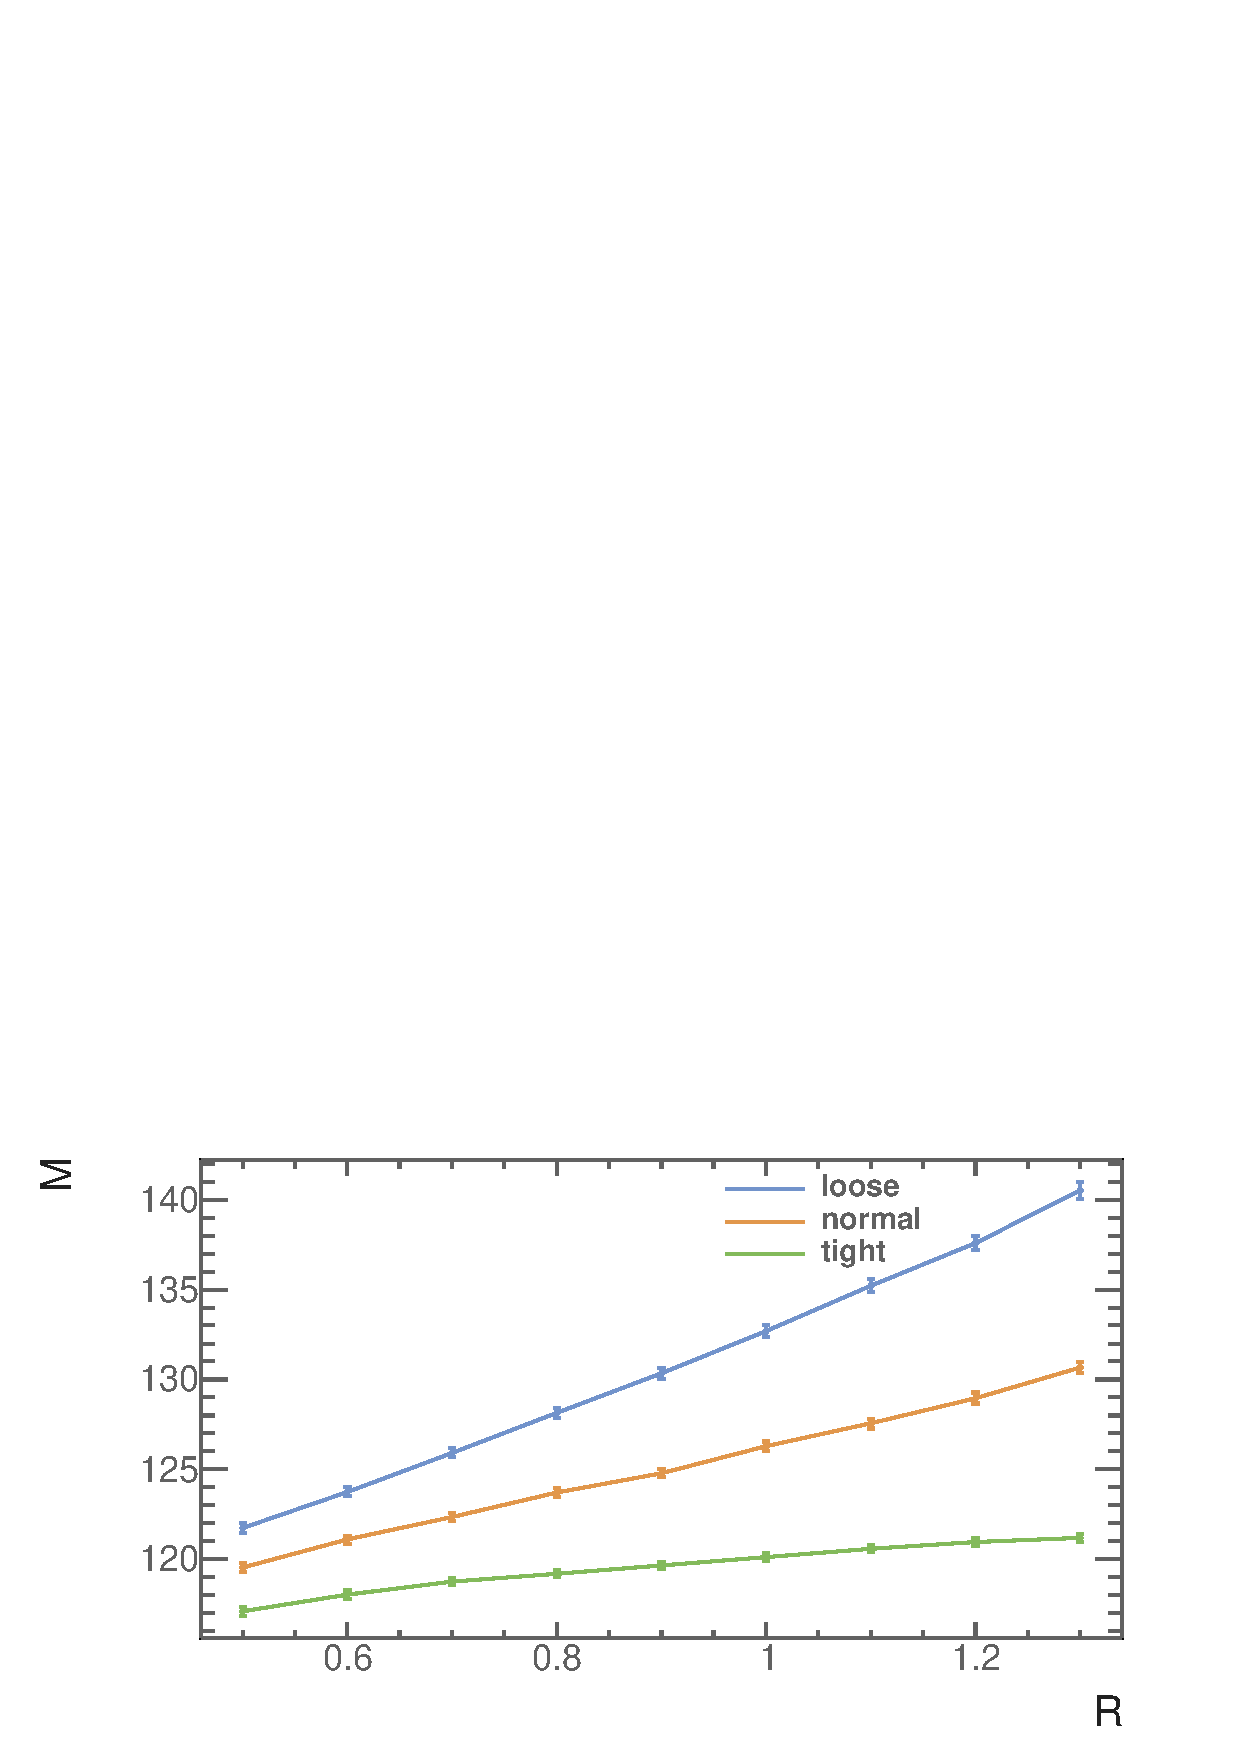
\includegraphics[width=\textwidth]{{doubleHiggs/resolution/ILD_1.4TeV_Higgs1_M_R}.pdf}
    \caption{}
    \label{fig:doubleHiggs1.4Higgs1M}
  \end{subfigure}
  \begin{subfigure}[b]{0.45\textwidth}
    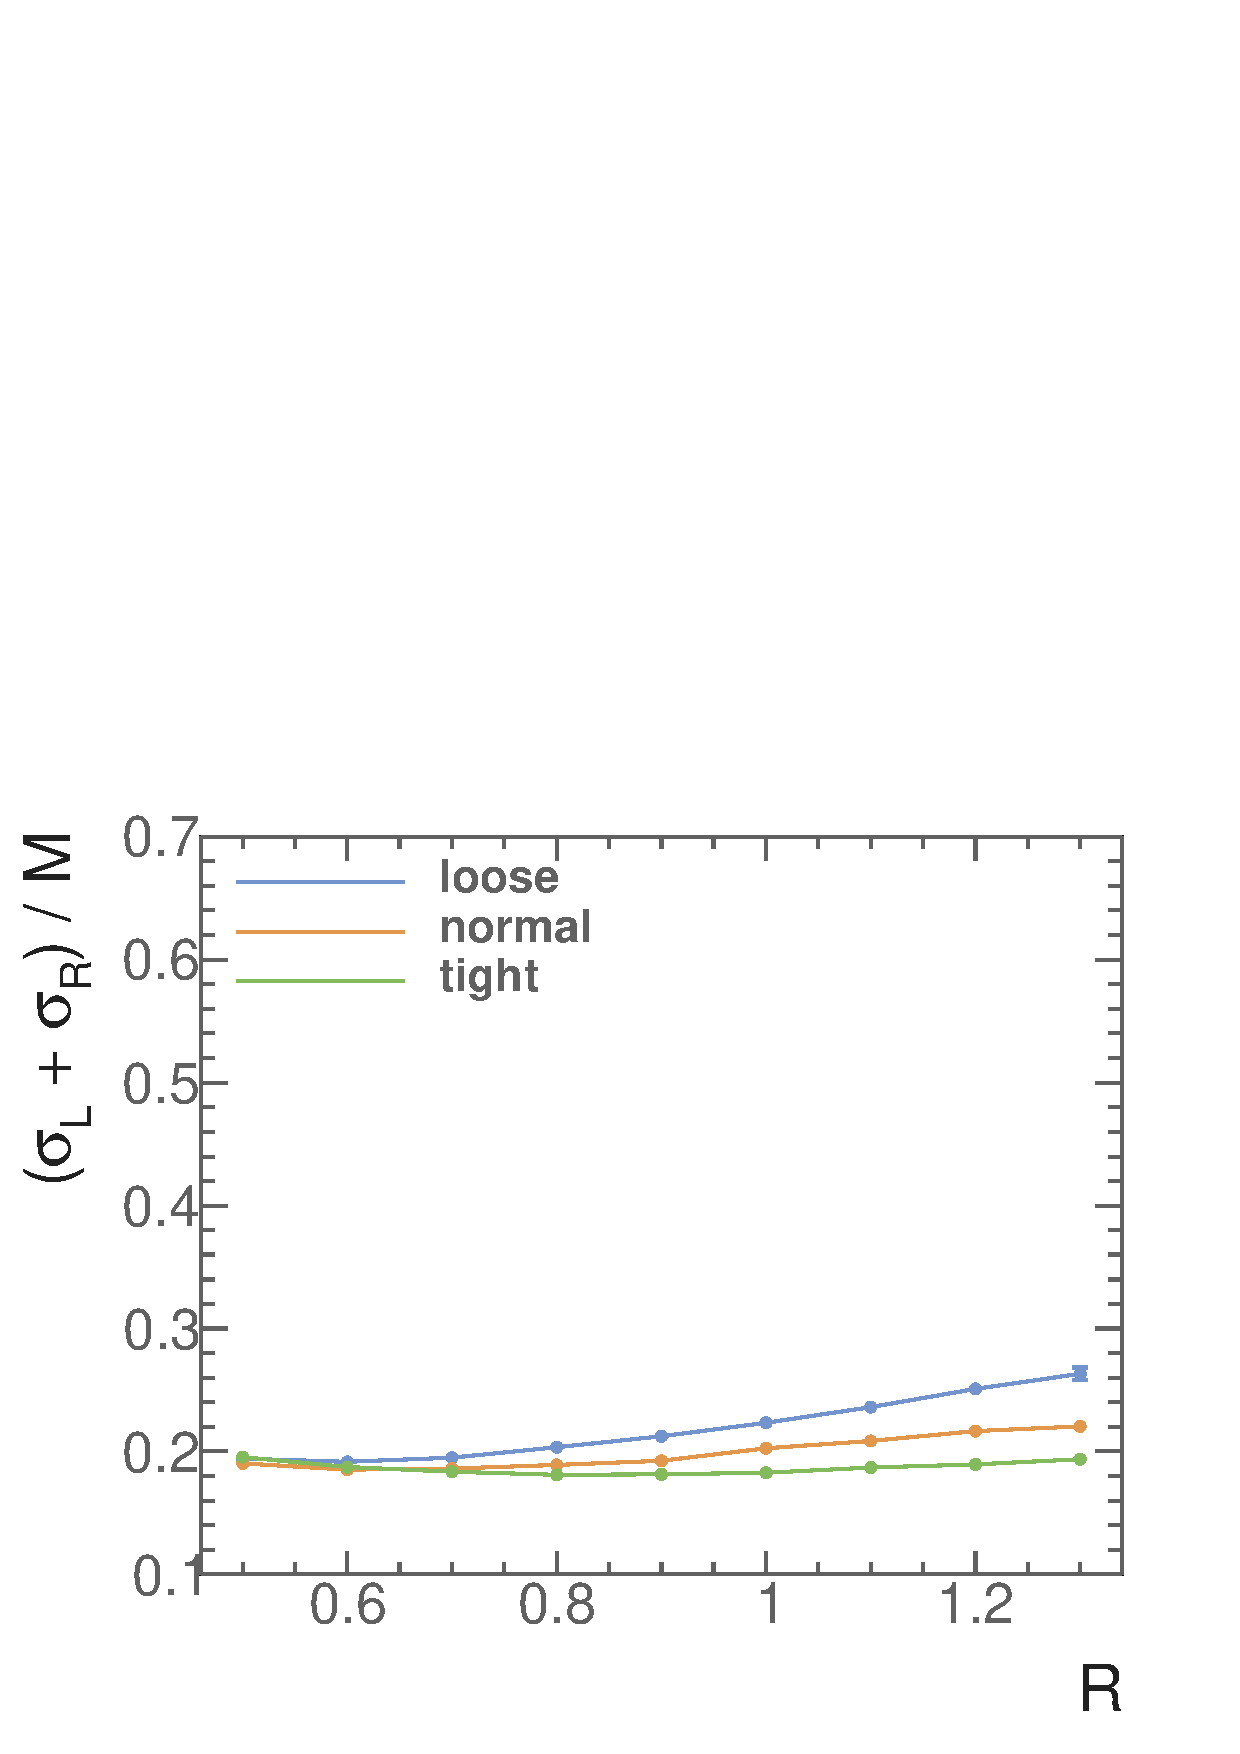
\includegraphics[width=\textwidth]{{doubleHiggs/resolution/ILD_1.4TeV_Higgs1_SigmaL_add_SigmaR_divide_M_testR}.pdf}
    \caption{}
    \label{fig:doubleHiggs1.4Higgs1Sigma}
  \end{subfigure}
  \begin{subfigure}[b]{0.45\textwidth}
    \includegraphics[width=\textwidth]{{doubleHiggs/resolution/ILD_1.4TeV_Higgs2_M_R}.pdf}
    \caption{}
    \label{fig:doubleHiggs1.4Higgs2M}
  \end{subfigure}
  \begin{subfigure}[b]{0.45\textwidth}
    \includegraphics[width=\textwidth]{{doubleHiggs/resolution/ILD_1.4TeV_Higgs2_SigmaL_add_SigmaR_divide_M_testR}.pdf}
    \caption{}
    \label{fig:doubleHiggs1.4Higgs2Sigma}
  \end{subfigure}
  \begin{subfigure}[b]{0.45\textwidth}
    \includegraphics[width=\textwidth]{{doubleHiggs/resolution/ILD_1.4TeV_W_M_testR}.pdf}
    \caption{}
    \label{fig:doubleHiggs1.4WM}
  \end{subfigure}
  \begin{subfigure}[b]{0.45\textwidth}
    \includegraphics[width=\textwidth]{{doubleHiggs/resolution/ILD_1.4TeV_W_SigmaL_add_SigmaR_divide_M_testR}.pdf}
    \caption{}
    \label{fig:doubleHiggs1.4WSigma}
  \end{subfigure}
\caption[Fitted mass, and resolution of \Hbb, \HWW and \PW at \rootS{1.4}]%
   {\FIGURE{fig:doubleHiggs1.4Higgs1M}, \ref{fig:doubleHiggs1.4Higgs2M}, and \ref{fig:doubleHiggs1.4WM}  show fitted mass peak positions of \Hbb, \HWW, and \PW as a function of $R$, for loose, normal and tight selected PFO collection at \rootS{1.4}. \FIGURE{fig:doubleHiggs1.4Higgs1Sigma}, \ref{fig:doubleHiggs1.4Higgs2Sigma}, and \ref{fig:doubleHiggs1.4WSigma} show relative mass peak width of \Hbb, \HWW, and \PW as a function of $R$  for loose, normal and tight selected \PFO collection at \rootS{1.4}.}
   \label{fig:doubleHiggs1.4TeVMassFit}
\end{figure}

\begin{table}[!htbp]
\begin{tabular}{lr}
\hline
\hline
Fitted jet parameters  &  \rootS{1.4}  \\
\hline
$\mu_{\Hbb}$ & $122.3_{\pm0.2}$  \\
$\sigma_{L,\Hbb}$ & $15.2_{\pm0.2}$   \\
$\sigma_{R,\Hbb}$ & $7.55_{\pm0.16}$   \\
\hline
$\mu_{\HWW}$ & $125.7_{\pm0.2}$   \\
$\sigma_{L,\HWW}$ & $29.4_{\pm0.3}$  \\
$\sigma_{R,\HWW}$ & $7.18_{\pm0.17}$ \\
\hline
$\mu_{\PW}$ & $80.5_{\pm0.2}$\\
$\sigma_{L,\PW}$ & $16.2_{\pm0.3}$  \\
$\sigma_{R,\PW}$ & $9.03_{\pm0.16}$  \\
\hline
\hline
\end{tabular}
\caption
[The fitted parameters of optimal jet reconstruction at \rootS{1.4}] %
{The fitted parameters of optimal jet reconstruction, \normalPFO with $R = 0.7$, at \rootS{1.4}.}
\label{tab:doubleHiggsFitParameters}
\end{table}

\section{Jet flavour tagging}
\label{sec:doubleHiggsFlavourTagging}

As the signal channel, \eeToHHbbWWHad,  has two \Pbottom quarks in the final state, identifying jets originated from \Pbottom quarks help to select signal events. To establish the likelihood of a \Pbottom jet, also known as \Pbottom tag value, \lcfiplus \cite{Suehara:2015ura} software package is used. An overview of the flavour tagging processor is provided in \Section{sec:pandoraLCFI}.

The flavour tagging is performed after the initial jet reconstruction using optimal jet reconstruction parameters.  \PFOs in the reconstructed jets are the inputs to the flavour tagging processor. \lcfiplus processor includes a multiclass classifier which needs to be trained. The samples for training the multiclass classifier are \HepProcess{\Pep \Pem \to \PZ \APnu \Pnu} at \rootS{1.4}, where \PZ decays to \HepProcess{\Pbottom\APbottom}, \HepProcess{\Pcharm\APcharm}, or \HepProcess{\Pup\APup/\Pdown\APdown/\Pstrange\APstrange}. At the training stage, the  jet clustering step is set to find two jets. The outputs for a jet is three values, corresponding to the likelihood of the jet being a b-jet, a c-jet, or a light flavour quark jet.  The selection efficiency of b jets and c jets with training samples is shown in \Figure{fig:doubleHiggs1.4Btag}.


\begin{figure}[!tbp]
    \includegraphics[width=0.45\textwidth]{{doubleHiggs/eval-lcfiweights_R0_7_2jets-test}.pdf}
    \caption
   {Performance of b-jet tagging with training samples at \rootS{1.4}.}
   \label{fig:doubleHiggs1.4Btag}
\end{figure}

To use the trained  multiclass classifier in the \lcfiplus processor, all the \PFOs in the initial reconstructed jet are fed into the processor. The jet clustering step in the \lcfiplus is set to find six jets. For each jet, values for the likelihood of a b-jet and a c-jet are obtained.

\section{Jet pairing}

Having optimised the jet reconstruction, and obtained the six jets from the jet clustering step in the \lcfiplus processor, the next step is to group jets according to event topology. Jets are paired up such that there are two jets for \HepProcess{\PHiggs \to \Pbottom \APbottom}, two jets for hadroinc decay of a \PW, two jets  for hadroinc decay  of a \W*, and the two $\PW{s}$ forming a  \PHiggs boson.
%off-mass-shell and off the mass shell? Is the "the" pertinent? Should they both be hyphenated?

The jet pairing scheme provides reconstructed invariant masses of \Hbb, \HWW, and \PW. The jet pairing metric states:
\begin{equation}
	\chi^2 = \left(\frac{m_{ij}-\mu_{\Hbb}}{\sigma_{\Hbb}^{\prime}}\right)^2 + \left(\frac{m_{klmn}-\mu_{\HWW}}{\sigma_{\HWW}^{\prime}}\right)^2  + \left(\frac{m_{kl}-\mu_{\PW}}{\sigma_{\PW}^{\prime}}\right)^2,
%\label{eqn:eq_chi2_HHWWbb}
\end{equation}

\begin{equation}
	\sigma_{\Hbb}^{\prime}=
    \begin{cases}
      \sigma_{L,\Hbb}, & \text{if}\ m_{ij} < \mu_{\Hbb}\\
     \sigma_{R,\Hbb}, & \text{otherwise} \\
   \end{cases}
\end{equation}

\begin{equation}
	\sigma_{\HWW}^{\prime}=
    \begin{cases}
      \sigma_{L,\HWW}, & \text{if}\ m_{klmn} < \mu_{\HWW}\\
     \sigma_{R,\HWW}, & \text{otherwise} \\
   \end{cases}
\end{equation}


\begin{equation}
	\sigma_{\PW}^{\prime}=
    \begin{cases}
      \sigma_{L,\PW}, & \text{if}\ m_{kl} < \mu_{\PW}\\
     \sigma_{R,\PW}, & \text{otherwise} \\
   \end{cases}
\end{equation}

where $i$ to $l$ indicate the one of the six jets with all possible combinations. $\mu$ and $\sigma$ are the fitted invariant mass and the fitted width from \Table{tab:doubleHiggsFitParameters}. The asymmetrical structure of the fitting function is reflected in the jet pairing metric. The paired jets with minimal $\chi^2$ is chosen with an additional requirement of at least one of two jets forming \Hbb having a \Pbottom-jet tag greater than 0.2.


\section{Pre-selection}
\label{sec:doubleHiggsPreSelection}
With reconstructed jets paired up, kinematic and topological variables can be calculated for the signal selection. A set of pre-selection cuts are placed to aid the multivariate analysis. The pre-selection cuts have three categories: discriminative pre-selection cuts, the mutually exclusive cuts with the \eeToHHbbqqqq sub-channel, and cuts to aid the MVA.

\subsection{Discriminative pre-selection cuts}

This set of  pre-selection cuts are designed to discard events that are dominated by background events. For the signal events, the double Higgs system have substantial invariant mass as both \PHiggs are on mass shell. The two \Pbottom jets in the signal final state are a clear signature. There is missing momentum as the final state contains neutrinos. The pre-selection cuts are listed in \Table{tab:doubleHiggsPreSel}. The distributions of variables used for discriminative pre-selection cuts are shown in \Figure{fig:doubleHiggs1.4TeVPreSelection}.

\FIGURE{fig:doubleHiggs1.4PreSelmHH} shows the distribution of the invariant mass of the two Higgs system, where the cut above 150\,GeV is effective against samples with two quark final states. \FIGURE{fig:doubleHiggs1.4PreSelbtag} shows the distribution of the second highest b-jet tag value, where the cut above 0.2 helps to reduce background events with no b-jets in final states. \FIGURE{fig:doubleHiggs1.4PreSelpT} shows the distribution of the transverse momentum  of the two Higgs system, where the cut above 30\,GeV  is extremely effective against background channels with no neutrinos in the final state.

\begin{table}[!htbp]
\begin{tabular}{lr}
\hline
\hline
Pre-selection  &  \rootS{1.4}  \\
\hline
Discriminative pre-selection & \multicolumn{1}{R{0.5\textwidth}}{$m_{\HH} > 150\,GeV$, $B_2 > 0.2$,  $\pT_{\HH} > 30\,GeV$} \\
Loose cuts for MVA &  \multicolumn{1}{R{0.5\textwidth}}{$m_{\Hbb} < 500\,GeV$, $m_{\HWW} < 800\,GeV$, $m_{\PW} < 200\,GeV$, $m_{\HH} < 1400\,GeV$} \\
Mutually exclusive & \sumBtag{4} < 2.3, \y{34} < 3.7 \\
\hline
\hline
\end{tabular}
\caption
{Pre-selection cuts at \rootS{1.4}.}
\label{tab:doubleHiggsPreSel}
\end{table}

\begin{figure}[!tbp]
  \begin{subfigure}[b]{0.45\textwidth}
    \includegraphics[width=\textwidth]{{doubleHiggs/preSel/nR0_7_6jet_btag2_Higgs_all_M_TMVA20161208R0_7_qq_btag2_prepare}.pdf}
    \caption{}
    \label{fig:doubleHiggs1.4PreSelmHH}
  \end{subfigure}
    \begin{subfigure}[b]{0.45\textwidth}
    \includegraphics[width=\textwidth]{{doubleHiggs/preSel/nR0_7_6jet_btag2_Higgs_all_Pt_TMVA20161208R0_7_qq_btag2_prepare}.pdf}
    \caption{}
    \label{fig:doubleHiggs1.4PreSelpT}
  \end{subfigure}
      \begin{subfigure}[b]{0.45\textwidth}
    \includegraphics[width=\textwidth]{{doubleHiggs/preSel/nR0_7_6jet_btag2_bTag2_TMVA20161208R0_7_qq_btag2_prepare}.pdf}
    \caption{}
    \label{fig:doubleHiggs1.4PreSelbtag}
  \end{subfigure}

\caption[Distributions of discriminative pre-selection variables for \rootS{1.4}.]%
   {Distributions of discriminative pre-selection variables for \rootS{1.4}. \Figure{fig:doubleHiggs1.4PreSelmHH},  \Figure{fig:doubleHiggs1.4PreSelpT}, and ,  \Figure{fig:doubleHiggs1.4PreSelbtag} show distributions for he invariant mass of the two Higgs system,  the second highest b-jet tag value, and the transverse momentum  of the two Higgs system respectively.}
   \label{fig:doubleHiggs1.4TeVPreSelection}
\end{figure}


\begin{table}[!tbp]\centering
% TODO fix lumi correction for e gamma, gamma e
% TODO change some of sample cross section for  electron-photon interaction with four quarks and a neutrino final state
%\small{
\small
\begin{tabular}{lrrrrr}
\hline \hline
 \multicolumn{1}{m{3.5cm}}{Channel / Efficiency \rootS{1.4}} &  \multicolumn{1}{m{2cm}}{Expected number of events}  & \multicolumn{1}{m{2cm}}{Lepton ID and jet pairing} & \multicolumn{1}{m{1.5cm}}{$m_{HH}>150\xspace{GeV}$} & \multicolumn{1}{m{1.5cm}}{$B_{2}>0.2$} & \multicolumn{1}{m{1.5cm}}{$\Pt>30\xspace{GeV}$}  \\
\hline
\eeToHH $\to$ \\
\HepProcess{ \Pbottom \APbottom \PWplus \PWminus \Pnue \APnue}, hadronic             &27.9& 85.8\% & 85.6\% & 73.7\%& 66.4\%\\
\hline
\eeToHH $\to$ \\
\HepProcess{ \Pbottom \APbottom \Pbottom \APbottom \Pnue \APnue}             &67.6& 90.8\% & 90.5\% & 90.1\% & 80.6\%\\
\eeToHH $\to$ other & 128.0 & 36.2\% & 35.3\% & 27.7\% & 24.7\%\\
\hline
\eeTo{\qlight \qlight \PHiggs \Pnu \APnu}  & 1304.0 & 60.7\% & 59.8\% & 44.9\%& 42.0\%\\
\eeTo{\Pcharm \APcharm \PHiggs \Pnu \APnu}  & 546.1 & 67.4\%& 57.7\%& 46.5\%& 43.4\%\\
\eeTo{\Pbottom \APbottom \PHiggs \Pnu \APnu}  & 463.0 & 73.9\%& 72.6\%& 68.7\%& 64.2\%\\

\eeTo{ \Pquark \Pquark \Pquark \Pquark}   &   1867650.0& 48.8\% & 46.1\%& 17.3\%& 4.7\%\\
\eeTo{ \Pquark \Pquark \Pquark \Pquark \Plepton \Plepton}& 93150.0 & 5.0\%& 4.9\%& 1.5\%& 0.3\%\\
\eeTo{ \Pquark \Pquark \Pquark \Pquark \Plepton \Pnu}& 165600.0 & 15.1\%& 15.1\%& 12.4\%& 11.4\%\\
\eeTo{ \Pquark \Pquark \Pquark \Pquark \Pnu \APnu} & 34800.0& 50.7\%& 50.0\%& 20.1\%& 18.8\%\\

\eeTo{ \Pquark \Pquark} &  6014250.0 & 54.5\%& 17.5\%& 8.4\%& 2.2\%\\
\eeTo{ \Pquark \Pquark \Plepton \Pnu} &  6464550.0 & 14.1\%& 5.3\%& 2.0\%& 1.6\%\\
\eeTo{ \Pquark \Pquark \Pl \Pl} &  4088700.0 & 13.0\%& 1.1\%& 0.6\%& 0.1\%\\
\eeTo{ \Pquark \Pquark \Pnu \Pnu} & 1181550.0 & 60.1\%& 12.3\%& 6.2\%& 5.8\% \\
\hline
\egamma{\Pepm}{\Pphoton}{BS}{\Pepm \Pquark \Pquark \Pquark \Pquark} & 2606625.5  & 23.3\%& 10.6\%& 4.4\%& 0.4\%\\
%\egamma{\Pem}{\Pphoton}{BS}{\Pem \Pquark \Pquark \Pquark \Pquark} & 1305787.5  & 23.3\%& 10.6\%& 4.4\%& 0.4\%\\
%\egamma{\Pep}{\Pphoton}{BS}{\Pep \Pquark \Pquark \Pquark \Pquark} & 1300837.5 & 23.4\%& 10.5\%& 4.3\%& 0.4\%\\
\egamma{\Pepm}{\Pphoton}{EPA}{\Pepm \Pquark \Pquark \Pquark \Pquark} & 861000.0 & 11.1\%& 5.4\%& 2.2\%& 0.3\%\\
%\egamma{\Pem}{\Pphoton}{EPA}{\Pem \Pquark \Pquark \Pquark \Pquark} & 430650.0 & 11.1\%& 5.4\%& 2.2\%& 0.3\%\\
%\egamma{\Pep}{\Pphoton}{EPA}{\Pep \Pquark \Pquark \Pquark \Pquark}  & 430350.0 & 11.1\% & 5.3\%& 2.1\%& 0.3\%\\
\egamma{\Pepm}{\Pphoton}{BS}{\Pnu \Pquark \Pquark \Pquark \Pquark}& 178987.5  & 58.0\%& 56.5\%& 30.7\%& 27.5\%\\
%\egamma{\Pem}{\Pphoton}{BS}{\Pnu \Pquark \Pquark \Pquark \Pquark}& 89775.0  & 58.3\%& 56.8\%& 31.0\%& 27.7\%\\
%\egamma{\Pep}{\Pphoton}{BS}{\APnu \Pquark \Pquark \Pquark \Pquark}& 89212.5 & 57.6\% & 56.1\%& 30.3\%& 27.3\%\\
\egamma{\Pepm}{\Pphoton}{EPA}{\Pnu \Pquark \Pquark \Pquark \Pquark}& 52050.0  & 29.4\% & 28.7\%& 15.2\%& 13.8\%\\
%\egamma{\Pem}{\Pphoton}{EPA}{\Pnu \Pquark \Pquark \Pquark \Pquark}& 26100.0  & 29.6\% & 28.9\%& 15.4\%& 13.9\%\\
%\egamma{\Pep}{\Pphoton}{EPA}{\APnu \Pquark \Pquark \Pquark \Pquark}& 25950.0  & 29.2\%& 28.5\%& 15.0\% & 13.7\%\\
\egamma{\Pepm}{\Pphoton}{BS}{\Pquark \Pquark \PHiggs \Pnu} & 35437.5  & 61.0\% & 59.9\%& 45.5\%& 34.6\%\\
%\egamma{\Pem}{\Pphoton}{BS}{\Pquark \Pquark \PHiggs \Pnu} & 17775  & 61.0\% & 59.8\%& 45.5\%& 34.6\%\\
%\egamma{\Pep}{\Pphoton}{BS}{\Pquark \Pquark \PHiggs \Pnu} & 17662.5  & 61.1\% & 60.0\% & 45.6\% & 34.6\%\\
\egamma{\Pepm}{\Pphoton}{EPA}{\Pquark \Pquark \PHiggs \Pnu} & 10170.0  & 31.8\% & 31.2\% & 23.7\%& 18.3\%\\
%\egamma{\Pem}{\Pphoton}{EPA}{\Pquark \Pquark \PHiggs \Pnu} & 5085  & 31.8\% & 31.2\% & 23.7\%& 18.2\%\\
%\egamma{\Pep}{\Pphoton}{EPA}{\Pquark \Pquark \PHiggs \Pnu} & 5085   & 31.9\% & 31.3\% & 23.8\% & 18.4\%\\
\hline
\gammagamma{\Pphoton}{BS}{\Pphoton}{BS}{ \Pquark \Pquark \Pquark \Pquark}& 2054951.5  & 56.3\%& 23.9\%& 9.6\%& 0.3\%\\
\gammagamma{\Pphoton}{BS}{\Pphoton}{EPA}{ \Pquark \Pquark \Pquark \Pquark}& 4521037.5  &33.6\%& 14.2\%& 5.7\%& 0.4\%\\
\gammagamma{\Pphoton}{EPA}{\Pphoton}{BS}{ \Pquark \Pquark \Pquark \Pquark}& 4539150.0 & 33.7\%& 14.2\%& 5.7\%& 0.4\%\\
\gammagamma{\Pphoton}{EPA}{\Pphoton}{EPA}{ \Pquark \Pquark \Pquark \Pquark}& 1129500.0 & 21.1\% & 9.1\% & 3.7\%& 0.4\%\\
\hline \hline
\end{tabular}

\caption[Pre-selection efficiencies at \rootS{1.4}.]%
{Pre-selection cut efficiencies for signal and background samples at \rootS{1.4}, assuming a luminosity of 1500\,$fb^{-1}$. The selection efficiencies are presented in a ``flow'' fashion. Every selection cut contains all the cuts to the left of it.}
\label{tab:doubleHiggs1.4TeVPreslection}
\end{table}

\subsection{Mutually exclusive cuts for \eeToHHbbWW and \eeToHHbbbb}
\label{sec:doubleHiggsMutualExclusive}
This set of cuts is designed to divide samples, both signal and background, into two mutually exclusive sets for the parallel analyses of  two sub-channels; \eeToHHbbWWHad and \eeToHHbbbb. This eases the difficulty of combining sub-channels as correlations between sub-channels need not to be considered where samples are mutually exclusive.

The most distinctive difference between the two sub-channels is the different number of jets and the different number of b-jets in the final state. Variables relating to the number of b-jets and number of overall jets are suitable for separating two sub-channels.

As demonstrated in \Figure{fig:doubleHiggsMutualPreselection}, two sub-channels can be clearly separated in the two dimensional parameter space. The optimal rectangular cuts were selected by scanning the two parameters and maximising a variant of Gini Index (see \Section{sec:pandoraDecisionTree}):
\begin{equation}
\varepsilon = P(subchannel_1|selection) \times P(subchannel_2|\neg{selection}),
\end{equation}
where $selection$ represents the phase space covered by the mutually exclusive cuts, $\neg{selection}$ indicates the phase space not covered by the $selection$.

Variables tested include \sumBtag{4}, \partialSumBtag{1}{3}{4}, \y{34}, \y{45}, \y{56}, \y{67}.  The \sumBtag{4} is the sum of the b-jet tag values when clustering an event into four jets. \y{} parameters measures the number of jets in an event (see \Section{sec:pandoraYparameter}). The performance of optimal  mutually exclusive cuts is summarised in \Table{tab:doubleHiggsMutualCuts}.

\begin{figure}[!tbp]
  \begin{subfigure}[b]{0.45\textwidth}
    \includegraphics[width=\textwidth]{{doubleHiggs/mutual6022bbWW}.pdf}
    \caption{\eeToHHbbWW, hadronic}
    \label{fig:doubleHiggs1.4MutualbbWW}
  \end{subfigure}
    \begin{subfigure}[b]{0.45\textwidth}
    \includegraphics[width=\textwidth]{{doubleHiggs/mutual6022bbbb}.pdf}
    \caption{\eeToHHbbbb}
    \label{fig:doubleHiggs1.4Mutualbbbb}
  \end{subfigure}
\caption[Sum of b-jet tag values as a function of $-\log\parenths{\y{34}}$ at \rootS{1.4}]%
   {[Sum of b-jet tag values as a function of $-\log\parenths{\y{34}}$ at \rootS{1.4}, shown for hadronic decay of \eeToHHbbWW and \eeToHHbbWW sub-channel. }
   \label{fig:doubleHiggsMutualPreselection}
\end{figure}

\begin{table}[!tbp]
\centering
\begin{tabular}{lrr}
\hline
\hline
Selection efficiency & \multicolumn{1}{R{0.4\textwidth}}{\eeToHHbbWW, hadronic} & \multicolumn{1}{R{0.3\textwidth}}{\eeToHHbbbb} \\
\sumBtag{4} < 2.3 and \y{34} < 3.7 & 86\% & 78\% \\
\hline
\hline
\end{tabular}
\caption[Mutually exclusive cuts at \rootS{1.4}.] %
{Events passed mutually exclusive cuts at \rootS{1.4} for hadronic decay of \eeToHHbbWW and \eeToHHbbbb sub-channels.}
\label{tab:doubleHiggsMutualCuts}
\end{table}

The selection efficiencies of signal and background events after mutually exclusive cuts are listed in \Table{tab:doubleHiggsPreslectionPart2}. As designed, the mutually exclusive cuts reject most \eeToHHbbbb events.

\begin{table}[!tbp]\centering
\small
\begin{tabular}{lrr}
\hline \hline
 \multicolumn{1}{L{0.3\textwidth}}{Channel} &  \multicolumn{1}{R{0.3\textwidth}}{Previous cuts and loose cuts}  & \multicolumn{1}{R{0.3\textwidth}}{Mutually exclusive} \\
\hline
\eeToHH $\to$ \\
\HepProcess{ \Pbottom \APbottom \PWplus \PWminus \Pnue \APnue}, hadronic             & 66.4\%& 59.7\% \\
\hline
\eeToHH $\to$ \\
\HepProcess{ \Pbottom \APbottom \Pbottom \APbottom \Pnue \APnue}             &80.6\%& 15.4\%  \\
\eeToHH $\to$ other & 24.7\% & 20.5\%  \\
\hline
\eeTo{\qlight \qlight \PHiggs \Pnu \APnu}  & 42.0\% & 39.5\% \\
\eeTo{\Pcharm \APcharm \PHiggs \Pnu \APnu}  & 43.4\% & 31.7\%\\
\eeTo{\Pbottom \APbottom \PHiggs \Pnu \APnu}  & 64.2\% & 25.2\%\\

\eeTo{ \Pquark \Pquark \Pquark \Pquark}   & 4.6\%  & 3.4\%\\
\eeTo{ \Pquark \Pquark \Pquark \Pquark \Plepton \Plepton}& 3.3\% & 3.1\%\\
\eeTo{ \Pquark \Pquark \Pquark \Pquark \Plepton \Pnu}& 11.4\%. & 9.8\%\\
\eeTo{ \Pquark \Pquark \Pquark \Pquark \Pnu \APnu} & 18.8\% & 16.6\%\\

\eeTo{ \Pquark \Pquark} &  2.0\% & 0.8\%\\
\eeTo{ \Pquark \Pquark \Plepton \Pnu} &  1.6\% & 0.9\%\\
\eeTo{ \Pquark \Pquark \Pl \Pl} &  0.1\% & 0.1\%\\
\eeTo{ \Pquark \Pquark \Pnu \Pnu} & 5.8\% & 4.0\%\\
\hline
\egamma{\Pepm}{\Pphoton}{BS}{\Pepm \Pquark \Pquark \Pquark \Pquark} & 0.4\%  & 0.3\%\\
%\egamma{\Pem}{\Pphoton}{BS}{\Pem \Pquark \Pquark \Pquark \Pquark} & 0.4\%  & 0.3\%\\
%\egamma{\Pep}{\Pphoton}{BS}{\Pep \Pquark \Pquark \Pquark \Pquark} & 0.4\% & 0.4\%\\
\egamma{\Pepm}{\Pphoton}{EPA}{\Pepm \Pquark \Pquark \Pquark \Pquark} & 0.3\% & 0.2\%\\
%\egamma{\Pem}{\Pphoton}{EPA}{\Pem \Pquark \Pquark \Pquark \Pquark} & 0.3\% & 0.2\%\\
%\egamma{\Pep}{\Pphoton}{EPA}{\Pep \Pquark \Pquark \Pquark \Pquark}  & 0.3\% & 0.3\% \\
\egamma{\Pepm}{\Pphoton}{BS}{\Pnu \Pquark \Pquark \Pquark \Pquark}& 27.5\%  & 25.6\%\\
%\egamma{\Pem}{\Pphoton}{BS}{\Pnu \Pquark \Pquark \Pquark \Pquark}& 27.7\%  & 25.3\%\\
%\egamma{\Pep}{\Pphoton}{BS}{\APnu \Pquark \Pquark \Pquark \Pquark}& 27.3\% & 24.9\% \\
\egamma{\Pem}{\Pphoton}{EPA}{\Pnu \Pquark \Pquark \Pquark \Pquark}&  13.8\% & 12.5\% \\
%\egamma{\Pem}{\Pphoton}{EPA}{\Pnu \Pquark \Pquark \Pquark \Pquark}&  13.9\% & 12.6\% \\
%\egamma{\Pep}{\Pphoton}{EPA}{\APnu \Pquark \Pquark \Pquark \Pquark}& 13.7\%  & 12.3\% \\
\egamma{\Pepm}{\Pphoton}{BS}{\Pquark \Pquark \PHiggs \Pnu} & 34.6\%  & 30.6\% \\
%\egamma{\Pem}{\Pphoton}{BS}{\Pquark \Pquark \PHiggs \Pnu} & 34.6\%  & 30.6\% \\
%\egamma{\Pep}{\Pphoton}{BS}{\Pquark \Pquark \PHiggs \Pnu} & 34.6\% & 30.6\%  \\
\egamma{\Pem}{\Pphoton}{EPA}{\Pquark \Pquark \PHiggs \Pnu} & 18.3\% & 16.0\%  \\
%\egamma{\Pem}{\Pphoton}{EPA}{\Pquark \Pquark \PHiggs \Pnu} & 18.2\% & 16.0\%  \\
%\egamma{\Pep}{\Pphoton}{EPA}{\Pquark \Pquark \PHiggs \Pnu} & 18.4\%   & 16.1\%  \\
\hline
\gammagamma{\Pphoton}{BS}{\Pphoton}{BS}{ \Pquark \Pquark \Pquark \Pquark}& 0.3\%  & 0.3\%\\
\gammagamma{\Pphoton}{BS}{\Pphoton}{EPA}{ \Pquark \Pquark \Pquark \Pquark}& 0.4\%  &0.3\%\\
\gammagamma{\Pphoton}{EPA}{\Pphoton}{BS}{ \Pquark \Pquark \Pquark \Pquark}& 0.4\% & 0.3\%\\
\gammagamma{\Pphoton}{EPA}{\Pphoton}{EPA}{ \Pquark \Pquark \Pquark \Pquark}& 0.4\% & 0.3\% \\
\hline \hline
\end{tabular}
\caption[List of signal and background samples after loose cuts and mutually exclusive cuts at \rootS{1.4}.]
{List of signal and background samples after loose cuts and mutually exclusive cuts at \rootS{1.4}. The selection efficiencies are presented in a ``flow'' fashion. Every selection cut contains all the cuts to the left of it.}
\label{tab:doubleHiggsPreslectionPart2}
\end{table}


\begin{comment}
    const TCut selectionCut3000 = "tR0_7_6jet_btag2_ChiSquared<20  && TightIsoLepTauAll_nPfo < 1 && BonoForwardElectronPhotons_nPfo < 1 && \
         tR0_7_6jet_btag2_Higgs_all_M>150  && \
       tR0_7_4jet_btag2_Higgs_all_bTag < 2.3 && tR0_7_6jet_btag2_minusLogY34 < 3.7 \
       && tR0_7_6jet_btag2_bTag1 > 0.7 &&\
        tR0_7_6jet_btag2_Higgs_all_M  < 3000 &&  tR0_7_6jet_btag2_Higgs1_M < 500 &&  tR0_7_6jet_btag2_Higgs2_M < 800 &&  tR0_7_6jet_btag2_W_Onshell_M < 200";

    const TCut selectionCut1400 = "nR0_7_6jet_btag2_ChiSquared<20  && IsoLepTauAll_nPfo < 1      && BonoForwardElectronPhotons_nPfo < 1 && nR0_7_6jet_btag2_Higgs_all_M>150 && \
        nR0_7_4jet_btag2_Higgs_all_bTag < 2.3  && nR0_7_6jet_btag2_minusLogY34 < 3.6 \
        &&  nR0_7_6jet_btag2_bTag2 > 0.2 && nR0_7_6jet_btag2_Higgs_all_Pt> 30 &&\
        nR0_7_6jet_btag2_Higgs_all_M  < 1400 &&  nR0_7_6jet_btag2_Higgs1_M < 500 &&  nR0_7_6jet_btag2_Higgs2_M < 800 &&  nR0_7_6jet_btag2_W_Onshell_M < 200";
\end{comment}

\subsection{Cuts to aid the MVA}

A set of physics-motivated cuts aims to reduce the range of invariant masses variables in order to increase the effectiveness of the MVA. (See \Section{sec:pandoraMVAbdtVar}). The invariant masses of physical bosons are required to be within a certain range to avoid the effect of extreme values on the MVA. The cuts are listed in \Table{tab:doubleHiggsPreSel} and the performance is shown in \Figure{tab:doubleHiggsPreslectionPart2}.


The selection efficiencies of all pre-selection cuts are shown in \Table{tab:doubleHiggs1.4TeVPreslection}. As the signal cross section is small compared to the background, only the signal events with very clear characteristic topologies would be selected by the MVA. Therefore, pre-selection cuts would not be detrimental to the final signal selection. On the contrary, pre-selection cuts improve the final signal selection efficiency as the MVA can focus on the difficult background events where their topologies are similar to the signal events.


\section{Discriminative variables for MVA}

A series of discriminative variables are calculated to differentiate the signal and background events. These variables are fed into MVA for signal selection. A full list of variables can be found in \Table{tab:doubleHiggsVaraibles}.

Invariant mass of $m_{\Hbb}$ and $m_{\HWW}$ are very effective at selecting signal events as no background events have double Higgs bosons in final states. \FIGURE{fig:doubleHiggs1.4varMHbb} and \Figure{fig:doubleHiggs1.4varMHWW} show the distributions of $m_{\Hbb}$ and $m_{\HWW}$ after all pre-selection cuts.

For the off-shell \W*, its energy is used as its mass distribution does not have a resonance peak. The recoil momenta, which is calculated by assuming the collision at \sqrtS and a beam crossing angle of 20\,mrad. The pseudorapidity is used to describe the angle and focus on the forward region, defined as:
\begin{equation}
\eta \equiv  - \ln \left[ \tan \left( \frac{\theta}{2} \right) \right],
\end{equation}
where $\theta$ is the polar angle in a spherical polar coordinate system. Acollinearity, \acolinearity{12}, measures the angle between the two constituent jets, defined as:
\begin{equation}
\acolinearity{12} = \pi - \cos^{-1}\left(\textbf{\^{p}}_1\cdot\textbf{\^{p}}_2\right),
\end{equation}
where $\textbf{\^{p}}_1$ is the unit momentum three-vector of jet 1. \cosStar{12} is the cosine of the angle between the two constituent jets in their decay rest frame. \FIGURE{fig:doubleHiggs1.4varAcolHbb} and \Figure{fig:doubleHiggs1.4varSpinHbb} compares the \acolinearity{\Hbb} and  \cosStar{\Hbb}. Both show clear differences for the signal and background channels. For the signal, \cosStar{\Hbb} has a flat distribution, as expected from a back-to-back decay of \HepProcess{\PHiggs \to \Pbottom \APbottom}. For the background, \cosStar{\Hbb} peaks at 1.

The global event shape variables include \y{} variables (see \Section{sec:pandoraYparameter}), and the sphericity,  \sphericity. \sphericity is a measurement of the spherically symmetry of the event (see \Section{sec:pandoraEvtShape}).

The flavour tagging variables are discussed in \Section{sec:doubleHiggsFlavourTagging}. For example, \btagFull{1,\Hbb} denotes the highest b-jet tag value of two jets forming \Hbb. The number of \PFOs variables are effective against background events with fewer than six quarks in final states.

An optimal set of 32 variables are chosen for the best MVA performance, whilst no strong ($>80\%$) pair-wise correlation exists between any two variables. %shown in \Figure{fig:doubleHiggs1.4Corr}.


 \begin{table}[!tbp]\centering
\begin{tabular}{lr}
\hline
\hline
Category &  Variable \\
\hline
Invariant mass &  \multicolumn{1}{R{0.6\textwidth}}{$m_{\Hbb}$, $m_{\HWW}$, $m_{\PW}$, $m_{\HH}$} \\
Energy and momentum & \multicolumn{1}{R{0.6\textwidth}}{$E_{\W*}$, $E_{mis}$, $\pT_{\Hbb}$, $\pT_{\HWW}$, $\pT_{\PW}$, $\pT_{\HH}$} \\
Angles in lab frame & \multicolumn{1}{R{0.6\textwidth}}{$\eta_{mis}$, $\acolinearity{\Hbb}$, $\acolinearity{\PW}$, $\acolinearity{\HH}$} \\
Angles in boosted frames & \multicolumn{1}{R{0.6\textwidth}}{$\cosStar{\Hbb}$, $\cosStar{\HWW}$, $\cosStar{\PW}$, $\cosStar{\W*}$, $\cosStar{\HH}$} \\
Event shape & \multicolumn{1}{R{0.6\textwidth}}{$\abs{\sphericity}$, $-\ln(\y{23})$, $-\ln(\y{34})$, $-\ln(\y{45})$, $-\ln(\y{56})$} \\
\Pbottom and \Pcharm tag & \multicolumn{1}{R{0.6\textwidth}}{$\btagFull{1,\Hbb}$, $\btagFull{2,\Hbb}$, $\btagFull{1,\PW}$, $\btagFull{1,\W*}$, $\ctagFull{1,\Hbb}$, $\ctagFull{1,\PW}$} \\
Number of \PFOs &  \multicolumn{1}{R{0.6\textwidth}}{$\npfo{\Hbb}$, $\npfo{\HWW}$, $\npfo{\PW}$, $\npfo{\W*}$} \\
\hline
\hline
\end{tabular}
\caption
{Variables used in MVA at \rootS{1.4}}
\label{tab:doubleHiggsVaraibles}
\end{table}



 \begin{figure}[!tbp]
  \begin{subfigure}[b]{0.45\textwidth}
    \includegraphics[width=\textwidth]{{doubleHiggs/1400var/nR0_7_6jet_btag2_Higgs1_M_TMVA20161208R0_7_qq_btag2_prepare_testNew2}.pdf}
    \caption{}
    \label{fig:doubleHiggs1.4varMHbb}
  \end{subfigure}
    \begin{subfigure}[b]{0.45\textwidth}
    \includegraphics[width=\textwidth]{{doubleHiggs/1400var/nR0_7_6jet_btag2_Higgs2_M_TMVA20161208R0_7_qq_btag2_prepare_testNew2}.pdf}
    \caption{}
    \label{fig:doubleHiggs1.4varMHWW}
  \end{subfigure}
    \begin{subfigure}[b]{0.45\textwidth}
    \includegraphics[width=\textwidth]{{doubleHiggs/1400var/nR0_7_6jet_btag2_Higgs1_acolinearity_TMVA20161208R0_7_qq_btag2_prepare_testNew2}.pdf}
    \caption{}
    \label{fig:doubleHiggs1.4varAcolHbb}
  \end{subfigure}
    \begin{subfigure}[b]{0.45\textwidth}
    \includegraphics[width=\textwidth]{{doubleHiggs/1400var/nR0_7_6jet_btag2_Higgs1_spin_TMVA20161208R0_7_qq_btag2_prepare_testNew2}.pdf}
    \caption{}
    \label{fig:doubleHiggs1.4varSpinHbb}
  \end{subfigure}
\caption[Stacked plots of discriminative variables distributions used in the MVA at \rootS{1.4} after all pre-MVA cuts.]
   {Stacked plots of discriminative variables distributions used in the MVA at \rootS{1.4} after all pre-MVA cuts. \FIGURE{fig:doubleHiggs1.4varMHbb} and \Figure{fig:doubleHiggs1.4varMHWW} show the invariant mass distributions of \Hbb and \HWW. \FIGURE{fig:doubleHiggs1.4varAcolHbb} and \Figure{fig:doubleHiggs1.4varSpinHbb} show the acollinearity and the opening angle in the decay rest frame of the two jets forming \Hbb.}
   \label{fig:doubleHiggs1.4var}
\end{figure}

\begin{comment}
 \begin{figure}[!tbp]
  \begin{subfigure}[b]{0.45\textwidth}
    \includegraphics[width=\textwidth]{{doubleHiggs/mva/1400signalCorr}}
    \caption{}
    \label{fig:doubleHiggs1.4signalCorr}
  \end{subfigure}
    \begin{subfigure}[b]{0.45\textwidth}
    \includegraphics[width=\textwidth]{{doubleHiggs/mva/1400backgroundCorr}}
    \caption{}
    \label{fig:doubleHiggs1.4backgroundCorr}
  \end{subfigure}
\caption
   {The pair-wise correlation between discriminative variables for signal and background events at \rootS{1.4} after all pre-selection cuts.}
   \label{fig:doubleHiggs1.4Corr}
\end{figure}
\end{comment}

\section{Multivariate analysis}
\label{sec:doubleHiggsMVA}
After gathering information and applying  pre-selection cuts, signal events selection is performed using the multivariate analysis (MVA) with Boosted Decision Tree classifier (BDT). The parameters for boosted decision tree are optimised and checked for overtraining. A brief discussion on the MVA, classifier, and overtraining can be found in \Section{sec:pandoraMVA}.

The optimisation of the BDT follows the strategy outlined in \Section{sec:pandoraMVAbdtVar}. The optimised parameters are listed in \Table{tab:doubleHiggsBDTparameters}. The optimal values are obtained by choosing the best performance without overfitting.
%at \rootS{3}. The same optimised parameters are used for \rootS{1.4} analysis.

\begin{table}[!tbp]\centering
%\small{
\small
\begin{tabular}{lr}
\hline \hline
 Parameter &  Value \\
\hline
Depth of tree & 4 \\
Number of trees & 4000 \\
The minimum number of events in a node &  0.25\% of the total events \\
Boosting & adaptive boost \\
Learning rate of the adaptive boost & 0.5 \\
Metric for the optimal cuts & Gini Index \\
Bagging fraction & 0.5 \\
Number of bins per variables & 40 \\
End node output & x $\in [0,1]$ \\
Do-PreSelection & yes \\
\hline \hline
\end{tabular}

\caption
{Optimised parameters for the boosted decision tree classifier. See \Section{sec:pandoraMVAbdtVar} for detailed explanation of variables.}
\label{tab:doubleHiggsBDTparameters}
\end{table}

\begin{comment}
  "!H:!V:NTrees=4000:MinNodeSize=0.25%:MaxDepth=4:BoostType=RealAdaBoost:AdaBoostBeta=0.5:UseBaggedBoost:BaggedSampleFraction=0.5:SeparationType=GiniIndex:nCuts=40:DoPreselection=True" );
\end{comment}

Half of the samples were used for training, and the other half used for testing and classifier optimisation. The signal for the MVA is the hadronic decay of \eeToHH $\to$ \HepProcess{ \Pbottom \APbottom \PWplus \PWminus \Pnue \APnue}. \eeToHH decaying to other final states does not participate in the MVA training step. Although they are from the Feynman diagrams as the signal (see \Section{fig:doubleHiggsFeynman}), event topologies are different. They participate in the MVA applying stage.

\section{Signal selection results}
\label{sec:doubleHiggsSignalSelResult}
%first sentence doesn't make sense. Should there be an "and" in there?

Efficiencies of events passed the pre-selection cut and the MVA classifier are listed in \Table{tab:doubleHiggs1.4TeVMVA}, alongside with number of events after the MVA selection. A few  background channels have non-zero events after the MVA selection. \eeTo{\Pquark \APquark \PHiggs \Pnu \APnu} is difficult to discard because its topology, one single Higgs plus neutrino, is very similar to the signal event topology. Similarly, \eeTo{ \Pquark \Pquark \Pquark \Pquark \Plepton \Pnu} can be confused as the signal when the lepton is undetected in the forward region, or the lepton's energy is too low to be tagged. \eeTo{ \Pquark \Pquark \Pquark \Pquark \Pnu \APnu} can also have a similar topology to the signal. Other background channels that are not discarded after the MVA are the electron-photon and photon interactions with the same final states as the above channels.



Before interpreting the result at \rootS{1.4}, the analyses at \rootS{3} and  the semi-leptonic channel of \eeToHH $\to$ \HepProcess{ \Pbottom \APbottom \PWplus \PWminus \Pnue \APnue} are presented.

\begin{table}[!tbp]\centering
%\small{
\small
\begin{tabular}{lrrrr}
\hline \hline
 \multicolumn{1}{m{3.5cm}}{Channel / Efficiency \rootS{1.4}} &  \multicolumn{1}{m{2cm}}{N}  & \multicolumn{1}{m{2cm}}{$\varepsilon_{presel}$} & \multicolumn{1}{m{2cm}}{$\varepsilon_{MVA}$} & \multicolumn{1}{m{2cm}}{$N_{MVA}$} \\
\hline
\eeToHH $\to$ \\
\HepProcess{ \Pbottom \APbottom \PWplus \PWminus \Pnue \APnue}, hadronic             &27.9& 59.8\% & 8.2\% & 1.29 \\
\hline
\eeToHH $\to$ \\
\HepProcess{ \Pbottom \APbottom \Pbottom \APbottom \Pnue \APnue}             &67.6& 15.4\%  & 0.5\% & 0.05\\
\eeToHH $\to$ other                             & 128.0 & 20.4\% & 1.7\% & 0.45\\
\hline
\eeTo{\qlight \qlight \PHiggs \Pnu \APnu}  & 1304.0 & 39.5\% & 0.05\%& 0.29\\
\eeTo{\Pcharm \APcharm \PHiggs \Pnu \APnu}  & 546.1 & 31.6\%& 0.1\%& 0.16\\
\eeTo{\Pbottom \APbottom \PHiggs \Pnu \APnu}  & 463.0 & 24.7\%& 0.3\%& 0.37\\

\eeTo{ \Pquark \Pquark \Pquark \Pquark}   &   1867650.0& 3.3\% & - & -\\
\eeTo{ \Pquark \Pquark \Pquark \Pquark \Plepton \Plepton}& 93150.0 & 0.3\%& - &  - \\
\eeTo{ \Pquark \Pquark \Pquark \Pquark \Plepton \Pnu}& 165600.0 & 9.8\%& 0.01\%& 2.06\\
\eeTo{ \Pquark \Pquark \Pquark \Pquark \Pnu \APnu} & 34800.0& 16.5\%& 0.002\% & 0.10\\

\eeTo{ \Pquark \Pquark} &  6014250.0 & 0.8\%& - & - \\
\eeTo{ \Pquark \Pquark \Plepton \Pnu} &  6464550.0 & 0.9\%&  - & - \\
\eeTo{ \Pquark \Pquark \Pl \Pl} &  4088700.0 & 0.08\%& - & - \\
\eeTo{ \Pquark \Pquark \Pnu \Pnu} & 1181550.0 & 4.0\%& - & - \\
\hline
\egamma{\Pepm}{\Pphoton}{BS}{\Pepm \Pquark \Pquark \Pquark \Pquark} & 2606625.0  & 0.3\%& - & -\\
%\egamma{\Pem}{\Pphoton}{BS}{\Pem \Pquark \Pquark \Pquark \Pquark} & 1305787.5  & 0.3\%& - & -\\
%\egamma{\Pep}{\Pphoton}{BS}{\Pep \Pquark \Pquark \Pquark \Pquark} & 1300837.5 & 0.4\%& -& -\\
\egamma{\Pepm}{\Pphoton}{EPA}{\Pepm \Pquark \Pquark \Pquark \Pquark} & 861000.0 & 0.3\%&  - &  - \\
%\egamma{\Pem}{\Pphoton}{EPA}{\Pem \Pquark \Pquark \Pquark \Pquark} & 430650.0 & 0.3\%&  - &  - \\
%\egamma{\Pep}{\Pphoton}{EPA}{\Pep \Pquark \Pquark \Pquark \Pquark}  & 430350.0 & 0.3\% & - & -\\
\egamma{\Pepm}{\Pphoton}{BS}{\Pnu \Pquark \Pquark \Pquark \Pquark}& 178987.5  & 25.7\%& 0.005\%& 2.05\\
%\egamma{\Pem}{\Pphoton}{BS}{\Pnu \Pquark \Pquark \Pquark \Pquark}& 89775.0  & 25.4\%& 0.005\%& 1.09\\
%\egamma{\Pep}{\Pphoton}{BS}{\APnu \Pquark \Pquark \Pquark \Pquark}& 89212.5 & 24.9\% & 0.004\%& 0.96\\
\egamma{\Pepm}{\Pphoton}{EPA}{\Pnu \Pquark \Pquark \Pquark \Pquark}& 52050.0  & 12.5\% & 0.004\% & 0.27 \\
%\egamma{\Pem}{\Pphoton}{EPA}{\Pnu \Pquark \Pquark \Pquark \Pquark}& 26100.0  & 12.6\% & - &  - \\
%\egamma{\Pep}{\Pphoton}{EPA}{\APnu \Pquark \Pquark \Pquark \Pquark}& 25950.0  & 12.4\%& 0.008\% & 0.27\\
\egamma{\Pepm}{\Pphoton}{BS}{\Pquark \Pquark \PHiggs \Pnu} & 35437.5   & 30.7\% & 0.02\% & 2.16 \\
%\egamma{\Pem}{\Pphoton}{BS}{\Pquark \Pquark \PHiggs \Pnu} & 17775   & 30.8\% & 0.02\% & 1.00 \\
%\egamma{\Pep}{\Pphoton}{BS}{\Pquark \Pquark \PHiggs \Pnu} & 17662.5  & 30.6\% & 0.02\% & 1.16 \\
\egamma{\Pepm}{\Pphoton}{EPA}{\Pquark \Pquark \PHiggs \Pnu} & 10170.0  & 16.1\% & 0.06\% & 0.95 \\
%\egamma{\Pem}{\Pphoton}{EPA}{\Pquark \Pquark \PHiggs \Pnu} & 5085  & 16.0\% & 0.04\% & 0.33 \\
%\egamma{\Pep}{\Pphoton}{EPA}{\Pquark \Pquark \PHiggs \Pnu} & 5085   & 16.2\% & 0.08\% & 0.62 \\
\hline
\gammagamma{\Pphoton}{BS}{\Pphoton}{BS}{ \Pquark \Pquark \Pquark \Pquark}& 2054951.5  & 0.2\%&  - & -\\
\gammagamma{\Pphoton}{BS}{\Pphoton}{EPA}{ \Pquark \Pquark \Pquark \Pquark}& 4521037.5  & 0.4\%& - & - \\
\gammagamma{\Pphoton}{EPA}{\Pphoton}{BS}{ \Pquark \Pquark \Pquark \Pquark}& 4539150.0 & 0.3\%&  - & - \\
\gammagamma{\Pphoton}{EPA}{\Pphoton}{EPA}{ \Pquark \Pquark \Pquark \Pquark}& 1129500.0 & 0.3\% & - & -\\
\hline \hline
\end{tabular}

\caption[Selection efficiency and number of events for signal and background at \rootS{1.4}.]%
{List of signal and background samples with selection efficiency and number of events at \rootS{1.4}, assuming a luminosity of 1500$fb^{-1}$. The number of events, selection efficiency of pre-selection, selection efficiency of MVA after pre-selection, number of events after MVA are shown. - represents a number less than 0.01.}
\label{tab:doubleHiggs1.4TeVMVA}
\end{table}



\section{\eeToHH $\to$ \HepProcess{ \Pbottom \APbottom \PWplus \PWminus \Pnu \APnu} hadronic decay at \rootS{3} analysis}

The \eeToHH $\to$ \HepProcess{ \Pbottom \APbottom \PWplus \PWminus \Pnu \APnu} hadronic decay at \rootS{3} analysis follows the same strategy as the analysis at \rootS{1.4}. A brief discussion of each step and the results are provided and differences are highlighted. Cross sections of used samples are listed in \Table{tab:doubleHiggs3crossSection}.

\begin{table}[!tbp]\centering
% TODO fix lumi correction for e gamma, gamma e
% TODO change some of sample cross section for  electron-photon interaction with four quarks and a neutrino final state
\small
%{

\begin{tabular}{lrr}
\hline \hline
Channel  &  $\sigma(\rootS{3})$ / fb   \\
\hline
\eeToHH &0.588 \\
\hline
\eeToHHbbWWFull,hadronic &0.07 \\
\eeToHHbbbbFull  &0.19 \\
\eeToHHotherFull &0.34 \\
\hline
\eeTo{\qlight \qlight \PHiggs \Pnu \APnu} & 1.78 \\
\eeTo{\Pcharm \APcharm \PHiggs \Pnu \APnu} & 1.12\\
\eeTo{\Pbottom \APbottom \PHiggs \Pnu \APnu}  & 1.91\\

\eeTo{ \Pquark \Pquark \Pquark \Pquark} & 546.5*\\
\eeTo{ \Pquark \Pquark \Pquark \Pquark \Plepton \Plepton}&169.3*\\
\eeTo{ \Pquark \Pquark \Pquark \Pquark \Plepton \Pnu} &106.6*\\
\eeTo{ \Pquark \Pquark \Pquark \Pquark \Pnu \APnu}&71.5*\\

\eeTo{ \Pquark \Pquark} &2948.9\\
\eeTo{ \Pquark \Pquark \Plepton \Pnu} &5561.1\\
\eeTo{ \Pquark \Pquark \Pl \Pl}&3319.6\\
\eeTo{ \Pquark \Pquark \Pnu \Pnu} &1317.5 \\
\hline
\egamma{\Pepm}{\Pphoton}{BS}{\Pepm \Pquark \Pquark \Pquark \Pquark} & 2536.3*\\
%\egamma{\Pem}{\Pphoton}{BS}{\Pem \Pquark \Pquark \Pquark \Pquark} & 1268.7*\\
%\egamma{\Pep}{\Pphoton}{BS}{\Pep \Pquark \Pquark \Pquark \Pquark}  & 1267.6*\\
\egamma{\Pepm}{\Pphoton}{EPA}{\Pepm \Pquark \Pquark \Pquark \Pquark}  & 575.7*\\
%\egamma{\Pem}{\Pphoton}{EPA}{\Pem \Pquark \Pquark \Pquark \Pquark}  & 287.9*\\
%\egamma{\Pep}{\Pphoton}{EPA}{\Pep \Pquark \Pquark \Pquark \Pquark}   & 287.8*\\
\egamma{\Pepm}{\Pphoton}{BS}{\Pnu \Pquark \Pquark \Pquark \Pquark}  & 524.8*\\
%\egamma{\Pem}{\Pphoton}{BS}{\Pnu \Pquark \Pquark \Pquark \Pquark}  & 262.5*\\
%\egamma{\Pep}{\Pphoton}{BS}{\APnu \Pquark \Pquark \Pquark \Pquark} & 262.3*\\
\egamma{\Pepm}{\Pphoton}{EPA}{\Pnu \Pquark \Pquark \Pquark \Pquark}  & 108.4*\\
%\egamma{\Pem}{\Pphoton}{EPA}{\Pnu \Pquark \Pquark \Pquark \Pquark}  & 54.2*\\
%\egamma{\Pep}{\Pphoton}{EPA}{\APnu \Pquark \Pquark \Pquark \Pquark}& 54.2*\\
\egamma{\Pepm}{\Pphoton}{BS}{\Pquark \Pquark \PHiggs \Pnu}   & 117.1* \\
%\egamma{\Pem}{\Pphoton}{BS}{\Pquark \Pquark \PHiggs \Pnu}   & 58.6* \\
%\egamma{\Pep}{\Pphoton}{BS}{\Pquark \Pquark \PHiggs \Pnu}  & 58.5* \\
\egamma{\Pepm}{\Pphoton}{EPA}{\Pquark \Pquark \PHiggs \Pnu} & 22.4* \\
%\egamma{\Pem}{\Pphoton}{EPA}{\Pquark \Pquark \PHiggs \Pnu} & 11.7* \\
%\egamma{\Pep}{\Pphoton}{EPA}{\Pquark \Pquark \PHiggs \Pnu} & 11.7* \\
\hline
\gammagamma{\Pphoton}{BS}{\Pphoton}{BS}{ \Pquark \Pquark \Pquark \Pquark}&13050.3*\\
\gammagamma{\Pphoton}{BS}{\Pphoton}{EPA}{ \Pquark \Pquark \Pquark \Pquark}&2420.6*\\
\gammagamma{\Pphoton}{EPA}{\Pphoton}{BS}{ \Pquark \Pquark \Pquark \Pquark}&2423.1*\\
\gammagamma{\Pphoton}{EPA}{\Pphoton}{EPA}{ \Pquark \Pquark \Pquark \Pquark}&402.7* \\
\hline \hline
\end{tabular}

\caption[Cross sections of samples at \rootS{3}.]
{List of signal and background samples with the corresponding cross sections at \rootS{3}. \Pquark can be \Pup, \Pdown, \Pstrange, \Pbottom or \Ptop. Unless specified, \Pquark, \Plepton and \Pnu represent particles and their corresponding anti-particles. \Pphoton(BS) represents a real photon from beamsstrahlung (BS). \Pphoton(EPA) represents a ``quasi-real'' photon simulated with the Equivalent Photon Approximation. For processes involving Higgs production explicitly, simulated Higgs mass is 126\,GeV. Otherwise, Higgs mass is set to 14\,TeV. For processes labelled with *, the generator level cut requires invariant mass of quarks greater than 50\,GeV.}
\label{tab:doubleHiggs3crossSection}
\end{table}

The lepton finding processors are either developed or optimised with samples at \rootS{1.4}, and checked with samples at \rootS{3} (see \Section{sec:doubleHiggsLepton}).  It was found that the same set of parameters for lepton identifiers works well under \rootS{1.4} and 3\,TeV. The performance of the lepton processors is shown in \Table{tab:doubleHiggs3TeVIsoLepPerformance}.

\begin{table}[!tbp]
\begin{tabular}{lrr}
\hline
\hline
Efficiency (3\,TeV)  &  Signal  & \HepProcess{\Pep \Pem \to \Pquark\Pquark\Pquark\Pquark\Plepton\Pnu} \\
\hline
\IsolatedLeptonFinderProcessor & 99.5\% & 66.8\%  \\
\BonoLeptonFinder & 99.0\% & 52.5\%  \\
\TauFinderProcessor & 97.7\% & 79.5\%  \\
\BonoTauFinder & 86.3\% & 60.3\%  \\
Forward Finder Processors & 95.9\% & 80.7\%  \\
\hline
Combined & 81.0\% & 23.3\%  \\
\hline
\hline

\end{tabular}
\caption{Isolated lepton finder processors performance with the signal and selected background samples at \rootS{3}.}
\label{tab:doubleHiggs3TeVIsoLepPerformance}
\end{table}

%Would this read better if you explained why 1.4 is better rather than why 3 is worse? Better should be the focus, no?
When comparing \rootS{1.4} and \rootS{3}, the lepton finding performance is better for \rootS{1.4}. This is because at \rootS{3}, particles are  boosted and spatial separation between particles is smaller. The effect of high \sqrtS also reflects on the performance of the  ForwardFinderProcessor. Whilst at \rootS{1.4}, the processor only rejects 5\% \HepProcess{\Pep \Pem \to \Pquark\Pquark\Pquark\Pquark\Plepton\Pnu} background and 1\% signal, at \rootS{3} it rejects 19\% background and 4\% signal, as more primary leptons are in the forward region.

\begin{comment}
\begin{table}[!tbp]
\begin{tabular}{lrr}
\hline
\hline
Processor / Efficiency (3\,TeV)  &  Signal  & \egamma{\Pem}{\Pphoton}{BS}{\Pem \Pquark \Pquark \Pquark \Pquark}  \\
\hline
Combined light lepton finder & 84.4\% & 72.7\%  \\
ForwardFinderProcessor & 95.9\% & 55.4\%  \\
Combined & 81.0\% &  33.4\%  \\
\hline
\hline

\end{tabular}
\caption{Very forward electron and photon finder performance on the signal and selected background samples.}
\label{tab:doubleHiggs3TeVForwardPerformance}
\end{table}
\end{comment}

For the jet reconstruction optimisation, the same strategy outlined in \Section{sec:doubleHiggsJetOptimisation} is used. \FIGURE{fig:doubleHiggs3TeVMassFit} shows fitted mass peak positions for \Hbb, \HWW, and \PW, along with the relative mass resolutions. The relative resolution of \PW worsen with increasing $R$, hence optimal choice favours a small $R$ and \tightPFO. The optimal jet reconstruction parameters is  \tightPFO with $R = 0.7$. The excellent mass resolution with the optimal choice compensates for the invariant masses being slightly smaller than simulated values. The fitted mass peak positions and mass resolutions  1of the chosen jet reconstruction are listed in \Table{tab:doubleHiggs3TeVFitParameters}
% The optimal "what?" chosen is tight tightPFO?

\begin{figure}[!tbp]
  \begin{subfigure}[b]{0.45\textwidth}
    \includegraphics[width=\textwidth]{{doubleHiggs/resolution/ILD_3TeV_Higgs1_M_R}.pdf}
    \caption{}
    \label{fig:doubleHiggs3Higgs1M}
  \end{subfigure}
  \begin{subfigure}[b]{0.45\textwidth}
    \includegraphics[width=\textwidth]{{doubleHiggs/resolution/ILD_3TeV_Higgs1_SigmaL_add_SigmaR_divide_M_testR}.pdf}
    \caption{}
    \label{fig:doubleHiggs3Higgs1Sigma}
  \end{subfigure}
  \begin{subfigure}[b]{0.45\textwidth}
    \includegraphics[width=\textwidth]{{doubleHiggs/resolution/ILD_3TeV_Higgs2_M_R}.pdf}
    \caption{}
    \label{fig:doubleHiggs3Higgs2M}
  \end{subfigure}
  \begin{subfigure}[b]{0.45\textwidth}
    \includegraphics[width=\textwidth]{{doubleHiggs/resolution/ILD_3TeV_Higgs2_SigmaL_add_SigmaR_divide_M_testR}.pdf}
    \caption{}
    \label{fig:doubleHiggs3Higgs2Sigma}
  \end{subfigure}
  \begin{subfigure}[b]{0.45\textwidth}
    \includegraphics[width=\textwidth]{{doubleHiggs/resolution/ILD_3TeV_W_M_testR}.pdf}
    \caption{}
    \label{fig:doubleHiggs3WM}
  \end{subfigure}
  \begin{subfigure}[b]{0.45\textwidth}
    \includegraphics[width=\textwidth]{{doubleHiggs/resolution/ILD_3TeV_W_SigmaL_add_SigmaR_divide_M_testR}.pdf}
    \caption{}
    \label{fig:doubleHiggs3WSigma}
  \end{subfigure}
\caption[Fitted mass peak positions and relative mass resolution of \Hbb, \HWW and \PW at \rootS{3}.]%
   {\FIGURE{fig:doubleHiggs3Higgs1M}, \ref{fig:doubleHiggs3Higgs2M}, and \ref{fig:doubleHiggs3WM}  show fitted mass peak positions of \Hbb, \HWW, and \PW, respectively, for loose, normal and tight selected PFO collection as a function of $R$ at \rootS{3}. \FIGURE{fig:doubleHiggs3Higgs1Sigma}, \ref{fig:doubleHiggs3Higgs2Sigma}, and \ref{fig:doubleHiggs3WSigma} show relative mass resolutions of \Hbb, \HWW, and \PW, respectively, for loose, normal and tight selected \PFO collection as a function of  $R$ at \rootS{3}.}
   \label{fig:doubleHiggs3TeVMassFit}
\end{figure}

\begin{table}[!tbp]
\begin{tabular}{lrr}
\hline
\hline
Jet Parameters  & \rootS{3}  \\
\hline
$\mu_{\Hbb}$  & $119.1_{\pm0.3}$  \\
$\sigma_{L,\Hbb}$ & $15.0_{\pm0.3}$  \\
$\sigma_{R,\Hbb}$ & $8.4_{\pm0.2}$  \\
\hline
$\mu_{\HWW}$ &  $123.0_{\pm0.3}$  \\
$\sigma_{L,\HWW}$ & $36.6_{\pm0.6}$  \\
$\sigma_{R,\HWW}$ & $7.4_{\pm0.2}$  \\
\hline
$\mu_{\PW}$  & $78.1_{\pm0.3}$ \\
$\sigma_{L,\PW}$ & $13.1_{\pm0.4}$  \\
$\sigma_{R,\PW}$ &  $9.5_{\pm0.2}$  \\
\hline
\hline
\end{tabular}
\caption
[The extracted fitted parameters of optimal jet reconstructions at \rootS{3}.] %
{The extracted fitted parameters of optimal jet reconstructions for \tightPFO with $R = 0.7$ at \rootS{3}.}
\label{tab:doubleHiggs3TeVFitParameters}
\end{table}

The flavour tagging processor is trained with the optimal jet parameters at \rootS{3}. The performance of the flavour tagging  with training samples is shown in \Figure{fig:doubleHiggsBtag3TeV}. Comparing this to the performance at \rootS{1.4}, the performance is slightly worse, because at high \sqrtS, particles at more collimated and more difficult to separate.
%high energy or high energies?

\begin{figure}[!htbp]
    \includegraphics[width=0.45\textwidth]{{doubleHiggs/eval-lcfiweights_tR0_7_3000_2jets-test}.pdf}
    \caption
   {Performance of b-jet tagging with training samples at \rootS{3}.}
   \label{fig:doubleHiggsBtag3TeV}
\end{figure}

%why have the pre-selection cuts changed?
The pre-selection cuts at \rootS{3} are largely the same as ones for \rootS{1.4} analysis. The cuts are listed in \Table{tab:doubleHiggs3TeVPreSel}. The reason for using a different b-jet tag cut is because the performance of flavour tagging is worse at high \sqrtS. \FIGURE{fig:doubleHiggs3PreSelbtag} shows the distribution of the highest b-jet tag, where the cut above 0.7 helps to reduce background events with no b-jet in final states.  \FIGURE{fig:doubleHiggs3PreSelmHH} shows the distribution of the invariant mass of the two Higgs system, where the cut above 150\,GeV is effective against samples with two quark final states.

%The cut is aggressive to compensate for the worse performance of the flavour tagging at high \sqrtS.



\begin{table}[!htbp]
\begin{tabular}{lr}
\hline
\hline
Pre-selection  &  \rootS{3}  \\
\hline
Discriminative pre-selection & \multicolumn{1}{R{0.5\textwidth}}{$m_{\HH} > 150\,GeV$, $B_1 > 0.7$,  $\pT_{\HH} > 30\,GeV$} \\
Loose cuts for MVA &  \multicolumn{1}{R{0.5\textwidth}}{$m_{\Hbb} < 500\,GeV$, $m_{\HWW} < 800\,GeV$, $m_{\PW} < 200\,GeV$, $m_{\HH} <3000\,GeV$} \\
Mutually exclusive & \sumBtag{4} < 2.3, \y{34} < 3.6 \\
\hline
\hline
\end{tabular}
\caption
{Pre-selection cuts at \rootS{3}.}
\label{tab:doubleHiggs3TeVPreSel}
\end{table}

\begin{figure}[!tbp]
  \begin{subfigure}[b]{0.45\textwidth}
    \includegraphics[width=\textwidth]{{doubleHiggs/preSel/tR0_7_6jet_btag2_Higgs_all_M_TMVA201612083TeVtR0_7_qq_btag2_prepare}.pdf}
    \caption{}
    \label{fig:doubleHiggs3PreSelmHH}
  \end{subfigure}
    \begin{subfigure}[b]{0.45\textwidth}
    \includegraphics[width=\textwidth]{{doubleHiggs/preSel/tR0_7_6jet_btag2_bTag1_TMVA201612083TeVtR0_7_qq_btag2_prepare}.pdf}
    \caption{}
    \label{fig:doubleHiggs3PreSelbtag}
  \end{subfigure}
\caption[Distributions of variables used  in discriminative pre-selection cuts at \rootS{3}.]%
   {Distributions of variables used  in discriminative pre-selection cuts at \rootS{3}, after rejecting events with identified leptons and jet pairing.}
   \label{fig:doubleHiggs3TeVPreSelection}
\end{figure}

% The cut on $m_{HH}$ is effective against background with fewer number of quarks in the final states. The cut on $B_1$ is effective against final states with no b quark.


\begin{table}[!tbp]\centering
% TODO fix lumi correction for e gamma, gamma e
% TODO change some of sample cross section for  electron-photon interaction with four quarks and a neutrino final state
%\small{
\small
\begin{tabular}{lrrrr}
\hline \hline
 \multicolumn{1}{m{3.5cm}}{Channel / Efficiency \rootS{3}} &  \multicolumn{1}{m{2cm}}{Expected number of events}  & \multicolumn{1}{m{2cm}}{Lepton ID and jet pairing} & \multicolumn{1}{m{1.5cm}}{$m_{HH}>150\xspace{GeV}$} & \multicolumn{1}{m{1.5cm}}{$B_{1}>0.7$} \\
\hline
\eeToHH $\to$ \\
\HepProcess{ \Pbottom \APbottom \PWplus \PWminus \Pnue \APnue}, hadronic             &146.0& 80.2\% & 79.9\% & 69.7\%\\
\hline
\eeToHH $\to$ \\
\HepProcess{ \Pbottom \APbottom \Pbottom \APbottom \Pnue \APnue}             &355.0& 83.4\% & 82.9\% & 81.2\% \\
\eeToHH $\to$ other & 675.0 & 36.7\% & 35.8\% & 25.2\% \\
\hline
\eeTo{\qlight \qlight \PHiggs \Pnu \APnu}  & 6115.4 & 59.5\% & 58.5\% & 40.4\%\\
\eeTo{\Pcharm \APcharm \PHiggs \Pnu \APnu}  & 2249.9 & 64.8\%& 58.4\%& 39.3\%\\
\eeTo{\Pbottom \APbottom \PHiggs \Pnu \APnu}  & 2197.7 & 69.7\%& 68.4\%& 64.2\%\\

\eeTo{ \Pquark \Pquark \Pquark \Pquark}   &   1093000.0& 48.5\% & 39.7\%& 3.0\%\\
\eeTo{ \Pquark \Pquark \Pquark \Pquark \Plepton \Plepton}& 338600.0 & 14.7\%& 14.2\%& 0.7\%\\
\eeTo{ \Pquark \Pquark \Pquark \Pquark \Plepton \Pnu}& 213200.0 & 19.7\%& 19.4\%& 10.0\%\\
\eeTo{ \Pquark \Pquark \Pquark \Pquark \Pnu \APnu} & 143000.0& 58.4\%& 57.3\%& 11.9\%\\

\eeTo{ \Pquark \Pquark} &  5897800.0 & 62.8\%& 13.2\%& 2.7\%\\
\eeTo{ \Pquark \Pquark \Plepton \Pnu} &  11121800 & 28.3\%& 11.9\%& 0.3\%\\
\eeTo{ \Pquark \Pquark \Pl \Pl} &  6639200.0 & 38.3\%& 2.9\%& 0.7\%\\
\eeTo{ \Pquark \Pquark \Pnu \Pnu} & 2635000.0 & 71.4\%& 24.1\%& 5.3\% \\
\hline
\egamma{\Pepm}{\Pphoton}{BS}{\Pepm \Pquark \Pquark \Pquark \Pquark} & 4006722.2  & 23.3\%& 21.5\%& 0.8\%\\
%\egamma{\Pem}{\Pphoton}{BS}{\Pem \Pquark \Pquark \Pquark \Pquark} & 2004388.1  & 23.3\%& 21.5\%& 0.8\%\\
%\egamma{\Pep}{\Pphoton}{BS}{\Pep \Pquark \Pquark \Pquark \Pquark} & 2002334.1 & 23.4\%& 21.6\%& 0.8\%\\
\egamma{\Pepm}{\Pphoton}{EPA}{\Pepm \Pquark \Pquark \Pquark \Pquark} & 1151200.0& 12.0\%& 11.0\%& 0.5\%\\
%\egamma{\Pem}{\Pphoton}{EPA}{\Pem \Pquark \Pquark \Pquark \Pquark} & 575600.0& 12.0\%& 11.0\%& 0.5\%\\
%\egamma{\Pep}{\Pphoton}{EPA}{\Pep \Pquark \Pquark \Pquark \Pquark}  & 575600.0 & 12.0\% & 10.9\%& 0.4\%\\
\egamma{\Pepm}{\Pphoton}{BS}{\Pnu \Pquark \Pquark \Pquark \Pquark}& 829184.0  & 61.5\%& 59.3\%& 19.9\%\\
%\egamma{\Pem}{\Pphoton}{BS}{\Pnu \Pquark \Pquark \Pquark \Pquark}& 414750.0  & 61.7\%& 59.5\%& 20.4\%\\
%\egamma{\Pep}{\Pphoton}{BS}{\APnu \Pquark \Pquark \Pquark \Pquark}& 414434.0 & 61.2\% & 59.1\%& 19.4\%\\
\egamma{\Pepm}{\Pphoton}{EPA}{\Pnu \Pquark \Pquark \Pquark \Pquark}& 216800.0  & 30.8\% & 29.8\%& 9.4\%\\
%\egamma{\Pem}{\Pphoton}{EPA}{\Pnu \Pquark \Pquark \Pquark \Pquark}& 108400.0  & 30.9\% & 29.9\%& 9.6\%\\
%\egamma{\Pep}{\Pphoton}{EPA}{\APnu \Pquark \Pquark \Pquark \Pquark}& 108400.0  & 30.7\%& 29.7\%& 9.1\% \\
\egamma{\Pepm}{\Pphoton}{BS}{\Pquark \Pquark \PHiggs \Pnu} & 185018.0  & 58.2\% &56.1\%& 37.2\% \\
%\egamma{\Pem}{\Pphoton}{BS}{\Pquark \Pquark \PHiggs \Pnu} & 92588.0  & 58.3\% &56.2\%& 37.3\% \\
%\egamma{\Pep}{\Pphoton}{BS}{\Pquark \Pquark \PHiggs \Pnu} & 92430.0 & 58.1\% & 56.0\% & 37.1\% \\
\egamma{\Pepm}{\Pphoton}{EPA}{\Pquark \Pquark \PHiggs \Pnu} & 46800.0 & 29.9\% &28.9\% & 19.1\% \\
%\egamma{\Pem}{\Pphoton}{EPA}{\Pquark \Pquark \PHiggs \Pnu} & 23400.0 & 30.1\% &29.2\% & 19.4\% \\
%\egamma{\Pep}{\Pphoton}{EPA}{\Pquark \Pquark \PHiggs \Pnu} & 23400.0   & 29.7\% & 28.6\% & 18.8\% \\
\hline
\gammagamma{\Pphoton}{BS}{\Pphoton}{BS}{ \Pquark \Pquark \Pquark \Pquark}& 18009413.9  & 54.2\%& 49.2\%& 1.9\%\\
\gammagamma{\Pphoton}{BS}{\Pphoton}{EPA}{ \Pquark \Pquark \Pquark \Pquark}& 3824548.1  &33.5\%& 30.2\%& 1.2\%\\
\gammagamma{\Pphoton}{EPA}{\Pphoton}{BS}{ \Pquark \Pquark \Pquark \Pquark}& 3828498.1 & 33.7\%& 30.3\%& 1.2\%\\
\gammagamma{\Pphoton}{EPA}{\Pphoton}{EPA}{ \Pquark \Pquark \Pquark \Pquark}& 805400.0 & 22.0\% & 19.8\% & 0.8\%\\
\hline \hline
\end{tabular}

\caption[Signal and background events with selection efficiency and event numbers after the pre-selection cuts at \rootS{3}]%
{List of signal and background samples with selection efficiencies and event numbers after the pre-selection cuts  at \rootS{3}, assuming a luminosity of 2000$fb^{-1}$. The selection efficiencies are presented in a ``flow'' fashion. Every selection cut contains all the cuts to the left of it.
}
\label{tab:doubleHiggs3TeVPreslection}
\end{table}

The cutsto aid the MVA at \rootS{3} are largely the same as the ones at \rootS{3}, apart from the difference on the cut of the invariant mass of \HH due to higher \sqrtS. The selection efficiency of the lepton veto and the pre-selection is shown in \Table{tab:doubleHiggs3TeVPreslection}.

The mutually exclusive cuts divide samples - both signal and background - into two mutually exclusive sets for the parallel analyses of  two subchannels; \eeToHHbbWWHad and \eeToHHbbbb. The cuts are obtained using the same strategy in \Section{sec:doubleHiggsMutualExclusive}. The cuts and efficiencies are listed in \Table{tab:doubleHiggs3TeVPreSel}. The two dimensional spaces for two sub-channels are shown in \Figure{fig:doubleHiggs3TeVMutualPreselection}. The selection efficiencies after the mutually exclusive cuts are shown in \Table{tab:doubleHiggs3TeVPreslectionPart2}.



\begin{figure}[!tbp]
  \begin{subfigure}[b]{0.45\textwidth}
    \includegraphics[width=\textwidth]{{doubleHiggs/mutual6025bbWW}.pdf}
    \caption{\eeToHHbbWW, hadronic}
    \label{fig:doubleHiggs3MutualbbWW}
  \end{subfigure}
    \begin{subfigure}[b]{0.45\textwidth}
    \includegraphics[width=\textwidth]{{doubleHiggs/mutual6025bbbb}.pdf}
    \caption{\eeToHHbbbb}
    \label{fig:doubleHiggs3Mutualbbbb}
  \end{subfigure}
\caption[Sum of b-jet tag as a function of \y{34} at \rootS{3}]%
   {Sum of b-jet tag as a function of \y{34} at \rootS{3}, shown for hadronic decay of \eeToHHbbWWHad and \eeToHHbbWW sub-channels. }
   \label{fig:doubleHiggs3TeVMutualPreselection}
\end{figure}

\begin{comment}
\begin{table}\centering
\begin{tabular}{llrr}
\hline
\hline
\sqrtS & $selection$ & \multicolumn{1}{m{4cm}}{\eeToHHbbqqqq Selection Efficiency} & \multicolumn{1}{m{4cm}}{\eeToHHbbbb Selection Efficiency} \\
1.4\,TeV &  \sumBtag{4} < 2.3 and \y{34} < 3.7 & 86\% & 78\% \\
3\,TeV &  \sumBtag{4} < 2.3 and \y{34} < 3.6 & 89\% & 82\% \\
\hline
\hline
\end{tabular}
\caption[Mutually exclusive cuts] %
{Mutually exclusive cuts, for full signal samples}
\label{tab:doubleHiggsMutualCuts}
\end{table}
\end{comment}

\begin{table}[!tbp]\centering
\small
\begin{tabular}{lrrrr}
\hline \hline
 \multicolumn{1}{L{0.3\textwidth}}{Channel} &  \multicolumn{1}{R{0.3\textwidth}}{Previous cuts and loose cuts}  & \multicolumn{1}{R{0.3\textwidth}}{Mutually exclusive} \\
\hline
\eeToHH $\to$ \\
\HepProcess{ \Pbottom \APbottom \PWplus \PWminus \Pnue \APnue}, hadronic             & 69.5\% & 61.7\%\\
\hline
\eeToHH $\to$ \\
\HepProcess{ \Pbottom \APbottom \Pbottom \APbottom \Pnue \APnue}             & 81.1\% & 18.8\% \\
\eeToHH $\to$ other & 25.1\% & 20.0\% \\
\hline
\eeTo{\qlight \qlight \PHiggs \Pnu \APnu}   & 40.3\% & 35.9\%\\
\eeTo{\Pcharm \APcharm \PHiggs \Pnu \APnu} & 39.2\%& 26.2\%\\
\eeTo{\Pbottom \APbottom \PHiggs \Pnu \APnu} & 64.2\%& 25.9\%\\

\eeTo{ \Pquark \Pquark \Pquark \Pquark}   & 2.5\%& 1.4\%\\
\eeTo{ \Pquark \Pquark \Pquark \Pquark \Plepton \Plepton} & 0.7\%& 0.6\%\\
\eeTo{ \Pquark \Pquark \Pquark \Pquark \Plepton \Pnu} & 9.2\%& 7.2\%\\
\eeTo{ \Pquark \Pquark \Pquark \Pquark \Pnu \APnu} & 11.8\%& 9.0\%\\

\eeTo{ \Pquark \Pquark} & 2.5\%& 1.4\%\\
\eeTo{ \Pquark \Pquark \Plepton \Pnu} & 0.3\%& 0.1\%\\
\eeTo{ \Pquark \Pquark \Pl \Pl} & 0.7\%& 0.4\%\\
\eeTo{ \Pquark \Pquark \Pnu \Pnu} & 5.3\%& 3.1\% \\
\hline
\egamma{\Pepm}{\Pphoton}{BS}{\Pepm \Pquark \Pquark \Pquark \Pquark}& 0.8\%& 0.7\%\\
%\egamma{\Pem}{\Pphoton}{BS}{\Pem \Pquark \Pquark \Pquark \Pquark}& 0.8\%& 0.7\%\\
%\egamma{\Pep}{\Pphoton}{BS}{\Pep \Pquark \Pquark \Pquark \Pquark} & 0.8\%& 0.7\%\\
\egamma{\Pepm}{\Pphoton}{EPA}{\Pepm \Pquark \Pquark \Pquark \Pquark} & 0.4\%& 0.4\%\\
%\egamma{\Pem}{\Pphoton}{EPA}{\Pem \Pquark \Pquark \Pquark \Pquark} & 0.4\%& 0.4\%\\
%\egamma{\Pep}{\Pphoton}{EPA}{\Pep \Pquark \Pquark \Pquark \Pquark}   & 0.4\%& 0.3\%\\
\egamma{\Pepm}{\Pphoton}{BS}{\Pnu \Pquark \Pquark \Pquark \Pquark} & 19.8\%& 16.4\%\\
%\egamma{\Pem}{\Pphoton}{BS}{\Pnu \Pquark \Pquark \Pquark \Pquark} & 20.3\%& 16.8\%\\
%\egamma{\Pep}{\Pphoton}{BS}{\APnu \Pquark \Pquark \Pquark \Pquark} & 19.3\%& 15.9\%\\
\egamma{\Pepm}{\Pphoton}{EPA}{\Pnu \Pquark \Pquark \Pquark \Pquark} & 9.2\%& 7.6\%\\
%\egamma{\Pem}{\Pphoton}{EPA}{\Pnu \Pquark \Pquark \Pquark \Pquark} & 9.4\%& 7.8\%\\
%\egamma{\Pep}{\Pphoton}{EPA}{\APnu \Pquark \Pquark \Pquark \Pquark}& 8.9\%& 7.3\% \\
\egamma{\Pepm}{\Pphoton}{BS}{\Pquark \Pquark \PHiggs \Pnu} &37.2\%& 30.2\% \\
%\egamma{\Pem}{\Pphoton}{BS}{\Pquark \Pquark \PHiggs \Pnu} &37.2\%& 30.2\% \\
%\egamma{\Pep}{\Pphoton}{BS}{\Pquark \Pquark \PHiggs \Pnu} & 37.1\% & 30.2\% \\
\egamma{\Pem}{\Pphoton}{EPA}{\Pquark \Pquark \PHiggs \Pnu} & 18.7\% & 15.5\% \\
%\egamma{\Pem}{\Pphoton}{EPA}{\Pquark \Pquark \PHiggs \Pnu} & 19.0\% & 15.7\% \\
%\egamma{\Pep}{\Pphoton}{EPA}{\Pquark \Pquark \PHiggs \Pnu} & 18.4\% & 15.2\% \\
\hline
\gammagamma{\Pphoton}{BS}{\Pphoton}{BS}{ \Pquark \Pquark \Pquark \Pquark}& 1.9\%& 1.7\%\\
\gammagamma{\Pphoton}{BS}{\Pphoton}{EPA}{ \Pquark \Pquark \Pquark \Pquark}& 1.1\%& 1.0\%\\
\gammagamma{\Pphoton}{EPA}{\Pphoton}{BS}{ \Pquark \Pquark \Pquark \Pquark}& 1.1\%& 1.0\%\\
\gammagamma{\Pphoton}{EPA}{\Pphoton}{EPA}{ \Pquark \Pquark \Pquark \Pquark} & 0.7\% & 0.6\%\\
\hline \hline
\end{tabular}
\caption[List of signal and background samples after loose cuts and mutually exclusive cuts at \rootS{3}.]
{List of signal and background samples with the selection efficiencies after loose cuts and mutually exclusive cuts at \rootS{3}. The selection efficiencies are presented in a ``flow'' fashion. Every selection cut contains all the cuts to the left of it.}
\label{tab:doubleHiggs3TeVPreslectionPart2}
\end{table}

The same set of variables for the MVA are used at \rootS{3} as in the analysis at \rootS{1.4}. The Boosted Decision Tree classifier is optimised at \rootS{3}. The efficiencies of the pre-selection cuts and the efficiencies of the MVA selections are listed in \Table{tab:doubleHiggs3TeVMVA}, alongside the number of events after the MVA selection. Background channels that are dominant after the MVA selection are almost identical to those at \rootS{1.4}. Hence see \Section{sec:doubleHiggsSignalSelResult} for discussion.

\begin{table}[!tbp]\centering
%\small{
\small
\begin{tabular}{lrrrr}
\hline \hline
 \multicolumn{1}{m{3.5cm}}{Channel / Efficiency \rootS{3}} &  \multicolumn{1}{m{2cm}}{N}  & \multicolumn{1}{m{2cm}}{$\varepsilon_{presel}$} & \multicolumn{1}{m{2cm}}{$\varepsilon_{MVA}$} & \multicolumn{1}{m{2cm}}{$N_{MVA}$} \\

\hline
\eeToHH $\to$ \\
\HepProcess{ \Pbottom \APbottom \PWplus \PWminus \Pnue \APnue}, hadronic             &146.0& 61.7\% & 11.6\% & 9.89\\
\hline
\eeToHH $\to$ \\
\HepProcess{ \Pbottom \APbottom \Pbottom \APbottom \Pnue \APnue}             &355.0& 18.8\% & 1.5\% & 1.05 \\
\eeToHH $\to$ other                             & 675.0 & 20.0\% & 3.6\% & 4.51 \\
\hline
\eeTo{\qlight \qlight \PHiggs \Pnu \APnu}  & 6115.4 & 36.0\% & 0.4\% & 9.42\\
\eeTo{\Pcharm \APcharm \PHiggs \Pnu \APnu}  & 2249.9 & 26.3\%& 0.5\%& 3.13\\
\eeTo{\Pbottom \APbottom \PHiggs \Pnu \APnu}  & 2197.7 & 25.8\%& 1.2\%& 6.82\\

\eeTo{ \Pquark \Pquark \Pquark \Pquark}   &   1093000.0& 1.4\% & 0.01\%& 1.43\\
\eeTo{ \Pquark \Pquark \Pquark \Pquark \Plepton \Plepton}& 338600.0 & 0.6\%&  - & -\\
\eeTo{ \Pquark \Pquark \Pquark \Pquark \Plepton \Pnu}& 213200.0 & 7.3\%& 0.05\%& 8.35\\
\eeTo{ \Pquark \Pquark \Pquark \Pquark \Pnu \APnu} & 143000.0& 9.0\%& 0.05\%& 6.35\\

\eeTo{ \Pquark \Pquark} &  5897800.0 & 1.4\%&  - & - \\
\eeTo{ \Pquark \Pquark \Plepton \Pnu} &  11121800 & 0.1\%& - & - \\
\eeTo{ \Pquark \Pquark \Pl \Pl} &  6639200.0 & 0.4\%& - & - \\
\eeTo{ \Pquark \Pquark \Pnu \Pnu} & 2635000.0 & 3.1\%&  - & - \\
\hline
\egamma{\Pepm}{\Pphoton}{BS}{\Pepm \Pquark \Pquark \Pquark \Pquark} & 4006722.2  & 0.7\%&  - & - \\
%\egamma{\Pem}{\Pphoton}{BS}{\Pem \Pquark \Pquark \Pquark \Pquark} & 2004388.1  & 0.7\%&  - & - \\
%\egamma{\Pep}{\Pphoton}{BS}{\Pep \Pquark \Pquark \Pquark \Pquark} & 2002334.1 & 0.7\%&  - & - \\
\egamma{\Pepm}{\Pphoton}{EPA}{\Pepm \Pquark \Pquark \Pquark \Pquark} & 1151200.0& 0.4\%&  - & - \\
%\egamma{\Pem}{\Pphoton}{EPA}{\Pem \Pquark \Pquark \Pquark \Pquark} & 575600.0& 0.4\%&  - & - \\
%\egamma{\Pep}{\Pphoton}{EPA}{\Pep \Pquark \Pquark \Pquark \Pquark}  & 575600.0 & 0.3\% &  - & - \\
\egamma{\Pepm}{\Pphoton}{BS}{\Pnu \Pquark \Pquark \Pquark \Pquark}& 829184.0  & 16.4\%& 0.04\%& 61.0\\
%\egamma{\Pem}{\Pphoton}{BS}{\Pnu \Pquark \Pquark \Pquark \Pquark}& 414750.0  & 16.8\%& 0.04\%& 30.7\\
%\egamma{\Pep}{\Pphoton}{BS}{\APnu \Pquark \Pquark \Pquark \Pquark}& 414434.0 & 15.9\% & 0.05\%& 30.3\\
\egamma{\Pepm}{\Pphoton}{EPA}{\Pnu \Pquark \Pquark \Pquark \Pquark}& 216800.0  & 7.6\% & 0.04\%& 6.0\\
%\egamma{\Pem}{\Pphoton}{EPA}{\Pnu \Pquark \Pquark \Pquark \Pquark}& 108400.0  & 7.8\% & 0.04\%& 3.37\\
%\egamma{\Pep}{\Pphoton}{EPA}{\APnu \Pquark \Pquark \Pquark \Pquark}& 108400.0  & 7.3\%& 0.03\%& 2.63 \\
\egamma{\Pepm}{\Pphoton}{BS}{\Pquark \Pquark \PHiggs \Pnu} & 185018.0  & 30.2\% & 0.2\%& 121.7 \\
%\egamma{\Pem}{\Pphoton}{BS}{\Pquark \Pquark \PHiggs \Pnu} & 92588.0  & 30.2\% & 0.2\%& 67.5 \\
%\egamma{\Pep}{\Pphoton}{BS}{\Pquark \Pquark \PHiggs \Pnu} & 92430.0 & 30.3\% & 0.2\% & 54.2 \\
\egamma{\Pepm}{\Pphoton}{EPA}{\Pquark \Pquark \PHiggs \Pnu} & 46800.0 & 15.3\% & 0.2\% & 18.1 \\
%\egamma{\Pem}{\Pphoton}{EPA}{\Pquark \Pquark \PHiggs \Pnu} & 23400.0 & 15.4\% & 0.2\% & 7.88 \\
%\egamma{\Pep}{\Pphoton}{EPA}{\Pquark \Pquark \PHiggs \Pnu} & 23400.0   & 15.2\% & 0.3\% & 10.2 \\
\hline
\gammagamma{\Pphoton}{BS}{\Pphoton}{BS}{ \Pquark \Pquark \Pquark \Pquark}& 18009413.9  & 1.6\%&   - & - \\
\gammagamma{\Pphoton}{BS}{\Pphoton}{EPA}{ \Pquark \Pquark \Pquark \Pquark}& 3824548.1  & 1.0\%&  - & - \\
\gammagamma{\Pphoton}{EPA}{\Pphoton}{BS}{ \Pquark \Pquark \Pquark \Pquark}& 3828498.1 & 1.0\%&  - & - \\
\gammagamma{\Pphoton}{EPA}{\Pphoton}{EPA}{ \Pquark \Pquark \Pquark \Pquark}& 805400.0 & 0.6\%&  - & - \\
\hline \hline
\end{tabular}
\caption[List of signal and background selection efficiencies and event numbers after MVA application at  \rootS{3}.]
{List of signal and background samples selection efficiencies and event numbers after MVA at  \rootS{3}, for a luminosity of 2000$fb^{-1}$. The number of events, selection efficiency of pre-selection, selection efficiency of MVA after pre-selection, number of events after MVA are shown. - represents a number less than 0.01.}
\label{tab:doubleHiggs3TeVMVA}
\end{table}

\section{\eeToHH $\to$ \HepProcess{ \Pbottom \APbottom \PWplus \PWminus \Pnu \APnu} semi-leptonic decay at \rootS{3} analysis}

The final analysis is on the \eeToHH $\to$ \HepProcess{ \Pbottom \APbottom \PWplus \PWminus \Pnu \APnu} semi-leptonic decay at \rootS{3}. The corresponding semi-leptonic analysis at \rootS{1.4} was also performed. Since the selected event number is too low, there are not enough signal events to have a meaningful discussion. Hence, only the analysis at \rootS{3} is presented.

The strategy of the analysis is very similar to the hadronic decay analysis. The main difference are that there is one lepton in the final state and the final state has four quarks instead of six. \Hbb and \PW can not be reconstructed due to the leptonic decay of one of the \PW. Hence, events are selected when there is one identified lepton using the same lepton finding processors. The jet reconstruction parameters are the same as hadronic decay analysis at the \rootS{3}. The pre-selection cuts are the same hadronic decay analysis at the \rootS{3}, with the performance listed in \Table{tab:doubleHiggs3TeVPreSelSemiLep}. There are no mutually exclusive cuts since there is no semi-leptonic analysis in the parallel analysis. Variables used in the MVA classifier are listed in \Table{tab:doubleHiggsVaraiblesSemiLep}. The efficiencies of the pre-selection cuts, the efficiencies of the MVA selections are listed in \Table{tab:doubleHiggsQlv3TeVMVA}, alongside the number of events after the MVA selection. Since there are three neutrinos in the final state, reconstructing the correct signal event topology is more difficult. The MVA performance is worse and almost all background channels are non-zero the MVA. Nevertheless,  dominant background channels are almost identical to those at \rootS{1.4}. Discussion of the results are provided in \Section{sec:doubleHiggsSignalSelResult}.
%"dominant background channels"?

\begin{table}[!htbp]
\begin{tabular}{lr}
\hline
\hline
Pre-selection  &  \rootS{3}  \\
\hline
Discriminative pre-selection & \multicolumn{1}{R{0.5\textwidth}}{$m_{\HH} > 150\,GeV$, $B_1 > 0.2$,  $\pT_{\HH} > 30\,GeV$} \\
Loose cuts for MVA &  \multicolumn{1}{R{0.5\textwidth}}{$m_{\Hbb} < 500\,GeV$, $m_{\HH} <3000\,GeV$} \\
\hline
\hline
\end{tabular}
\caption
{Pre-selection cuts at \rootS{3} for semi-leptonic analysis.}
\label{tab:doubleHiggs3TeVPreSelSemiLep}
\end{table}


 \begin{table}[!tbp]\centering
\begin{tabular}{lr}
\hline
\hline
Category &  Variable \\
\hline
Invariant mass &  \multicolumn{1}{R{0.6\textwidth}}{$m_{\Hbb}$, $m_{\PW}$, $m_{\HH}$} \\
Energy and momentum & \multicolumn{1}{R{0.6\textwidth}}{$E_{mis}$, $\pT_{\Hbb}$, $\pT_{\PW}$, $\pT_{\HH}$} \\
Angles in lab frame & \multicolumn{1}{R{0.6\textwidth}}{$\theta_{mis}$, $\acolinearity{\Hbb}$, $\acolinearity{\PW}$, $\acolinearity{\HH}$} \\
Angles in boosted frames & \multicolumn{1}{R{0.6\textwidth}}{$\cosStar{\Hbb}$, $\cosStar{\HH}$} \\
Event shape & \multicolumn{1}{R{0.6\textwidth}}{$\abs{\sphericity}$, $-\ln(\y{23})$, $-\ln(\y{34})$, $-\ln(\y{45})$, $-\ln(\y{56})$} \\
\Pbottom and \Pcharm tag & \multicolumn{1}{R{0.6\textwidth}}{$\btagFull{1,\Hbb}$, $\btagFull{2,\Hbb}$, $\btagFull{1,\PW}$, $\ctagFull{1,\Hbb}$, $\ctagFull{1,\PW}$} \\
Number of \PFOs &  \multicolumn{1}{R{0.6\textwidth}}{$\npfo{\Hbb}$, $\npfo{\PW}$} \\
\hline
\hline
\end{tabular}
\caption
{Variables used in MVA for semi-leptonic analysis  at \rootS{3}.}
\label{tab:doubleHiggsVaraiblesSemiLep}
\end{table}





\begin{table}[!tbp]\centering
%\small{
\small
\begin{tabular}{lrrrr}
\hline \hline
 \multicolumn{1}{m{3.5cm}}{Channel / Efficiency \rootS{1.4}} &  \multicolumn{1}{m{2cm}}{N}  & \multicolumn{1}{m{2cm}}{$\varepsilon_{presel}$} & \multicolumn{1}{m{2cm}}{$\varepsilon_{MVA}$} & \multicolumn{1}{m{2cm}}{$N_{MVA}$} \\
\hline
\eeToHH $\to$ \\
\HepProcess{ \Pbottom \APbottom \PWplus \PWminus \Pnue \APnue}, semi-leptonic       &96.8& 44.6\% & 21.9\% & 13.11\\
\hline
\eeToHH $\to$ \\
\HepProcess{ \Pbottom \APbottom \Pbottom \APbottom \Pnue \APnue}             &355.0& 13.3\% & 10.9\% &  5.38\\
\eeToHH $\to$ other                             & 724.2 & 13.1\% & 13.6\% &  12.75\\
\hline
\eeTo{\qlight \qlight \PHiggs \Pnu \APnu}  & 6115.4 & 7.4\% & 13.7\% & 62.63\\
\eeTo{\Pcharm \APcharm \PHiggs \Pnu \APnu}  & 2249.9 & 6.3\%& 12.1\%& 17.10\\
\eeTo{\Pbottom \APbottom \PHiggs \Pnu \APnu}  & 2197.7 & 15.9\%& 5.1\%& 18.03\\

\eeTo{ \Pquark \Pquark \Pquark \Pquark}   &   1093000.0& 0.6\% & 0.2\%& 15.04\\
\eeTo{ \Pquark \Pquark \Pquark \Pquark \Plepton \Plepton}& 338600.0 & 1.0\%&  0.06\% & 1.85\\
\eeTo{ \Pquark \Pquark \Pquark \Pquark \Plepton \Pnu}& 213200.0 & 27.6\%& 0.5\%& 270.33\\
\eeTo{ \Pquark \Pquark \Pquark \Pquark \Pnu \APnu} & 143000.0& 1.9\%& 1.6\%& 43.78\\

\eeTo{ \Pquark \Pquark} &  5897800.0 & 0.4\%&  0.3\% & 60.82 \\
\eeTo{ \Pquark \Pquark \Plepton \Pnu} &  11121800 & 0.3\%& 0.08\% & 21.24 \\
\eeTo{ \Pquark \Pquark \Pl \Pl} &  6639200.0 & 0.6\%& 0.2\%& 84.14\\
\eeTo{ \Pquark \Pquark \Pnu \Pnu} & 2635000.0 & 0.4\%&  0.9\% & 92.55 \\
\hline
\egamma{\Pepm}{\Pphoton}{BS}{\Pepm \Pquark \Pquark \Pquark \Pquark} & 4006722.2  & 1.2\%&  - & - \\
%\egamma{\Pem}{\Pphoton}{BS}{\Pem \Pquark \Pquark \Pquark \Pquark} & 2004388.1  & 1.2\%&  - & - \\
%\egamma{\Pep}{\Pphoton}{BS}{\Pep \Pquark \Pquark \Pquark \Pquark} & 2002334.1 & 1.2\%&  - & - \\
\egamma{\Pepm}{\Pphoton}{EPA}{\Pepm \Pquark \Pquark \Pquark \Pquark} & 1151200.0& 1.1\%&  - & - \\
%\egamma{\Pem}{\Pphoton}{EPA}{\Pem \Pquark \Pquark \Pquark \Pquark} & 575600.0& 1.1\%&  - & - \\
%\egamma{\Pep}{\Pphoton}{EPA}{\Pep \Pquark \Pquark \Pquark \Pquark}  & 575600.0 & 1.1\% &  - & - \\
\egamma{\Pepm}{\Pphoton}{BS}{\Pnu \Pquark \Pquark \Pquark \Pquark}& 829184.0  & 3.6\%& 1.5\%& 452.45\\
%\egamma{\Pem}{\Pphoton}{BS}{\Pnu \Pquark \Pquark \Pquark \Pquark}& 414750.0  & 3.7\%& 1.5\%& 226.77\\
%\egamma{\Pep}{\Pphoton}{BS}{\APnu \Pquark \Pquark \Pquark \Pquark}& 414434.0 & 3.5\% & 1.6\%& 225.68\\
\egamma{\Pepm}{\Pphoton}{EPA}{\Pnu \Pquark \Pquark \Pquark \Pquark}& 216800.0  & 11.0\% & 0.9\%& 200.65\\
%\egamma{\Pem}{\Pphoton}{EPA}{\Pnu \Pquark \Pquark \Pquark \Pquark}& 108400.0  & 11.2\% & 0.9\%& 107.90\\
%\egamma{\Pep}{\Pphoton}{EPA}{\APnu \Pquark \Pquark \Pquark \Pquark}& 108400.0  & 10.7\%& 0.8\%& 92.75 \\
\egamma{\Pepm}{\Pphoton}{BS}{\Pquark \Pquark \PHiggs \Pnu} & 185018.0  & 7.9\% & 10.4\%& 1521.93 \\
%\egamma{\Pem}{\Pphoton}{BS}{\Pquark \Pquark \PHiggs \Pnu} & 92588.0  & 7.9\% & 10.7\%& 779.36 \\
%\egamma{\Pep}{\Pphoton}{BS}{\Pquark \Pquark \PHiggs \Pnu} & 92430.0 & 7.9\% & 10.1\% & 741.57 \\
\egamma{\Pem}{\Pphoton}{EPA}{\Pquark \Pquark \PHiggs \Pnu} & 46800.0 & 22.8\% & 7.1\% & 750.85 \\
%\egamma{\Pem}{\Pphoton}{EPA}{\Pquark \Pquark \PHiggs \Pnu} & 23400.0 & 22.9\% & 6.9\% & 369.52 \\
%\egamma{\Pep}{\Pphoton}{EPA}{\Pquark \Pquark \PHiggs \Pnu} & 23400.0   & 22.7\% & 7.2\% & 381.33 \\
\hline
\gammagamma{\Pphoton}{BS}{\Pphoton}{BS}{ \Pquark \Pquark \Pquark \Pquark}& 18009413.9  & 0.4\%&   - & - \\
\gammagamma{\Pphoton}{BS}{\Pphoton}{EPA}{ \Pquark \Pquark \Pquark \Pquark}& 3824548.1  & 1.0\%&  - & - \\
\gammagamma{\Pphoton}{EPA}{\Pphoton}{BS}{ \Pquark \Pquark \Pquark \Pquark}& 3828498.1 & 1.0\%&  0.08\% & 28.85 \\
\gammagamma{\Pphoton}{EPA}{\Pphoton}{EPA}{ \Pquark \Pquark \Pquark \Pquark}& 805400.0 & 1.1\%&  - & - \\
\hline \hline
\end{tabular}
\caption[List of signal and background selection efficiencies and event numbers after MVA for semi-leptonic analysis at  \rootS{3}.]
{List of signal and background samples selection efficiencies and event numbers after MVA for semi-leptonic analysis at  \rootS{3}, assuming a luminosity of 2000$fb^{-1}$. The number of events, selection efficiency of pre-selection, selection efficiency of MVA after pre-selection, number of events after MVA are shown. - represents a number less than 0.01.}
\label{tab:doubleHiggsQlv3TeVMVA}
\end{table}

\section{Result interpretation}
\label{sec:doubleHiggsResults}

\begin{table}[!htbp]
\begin{tabular}{lrrr}
\hline
\hline
Channel  &  $N_{S}$ & $N_{B}$ & $N_S / \sqrt{N_S + N_B}$ \\
\hline
\multicolumn{1}{L{0.3\textwidth}}{\eeToHH $\to$ \HepProcess{ \Pbottom \APbottom \PWplus \PWminus \Pnue \APnue}, hadronic, \rootS{1.4}} & 1.79 & 8.41 & 0.56 \\
\multicolumn{1}{L{0.3\textwidth}}{\eeToHH $\to$ \HepProcess{ \Pbottom \APbottom \PWplus \PWminus \Pnue \APnue}, hadronic, \rootS{3}} & 15.45 & 242.28 & 0.96 \\
\multicolumn{1}{L{0.3\textwidth}}{\eeToHH $\to$ \HepProcess{ \Pbottom \APbottom \PWplus \PWminus \Pnue \APnue}, semi-leptonic, \rootS{3}} &  31.24& 3612.39 & 0.52 \\
\hline
\hline
\end{tabular}
\caption
{Number of signal and background events, and significance after MVA for all \eeToHHbbWW analyses.}
\label{tab:doubleHiggsResult}
\end{table}

The results of analyses at the \rootS{1.4} and \rootS{3}  are summarised in \Table{tab:doubleHiggsResult}. The expected precisions on the cross sections, which is roughly $\sqrt{N_S + N_B} / N_S$ at \rootS{1.4} and 3\,TeV, are:
\begin{equation}
\frac{\Delta\left[\sigma\left(\HHvv\right)\right]}{\sigma\left(\HHvv\right)}=
\begin{cases}
  179\%, & \mbox{at \rootS{1.4}, }  \\
  92\%, & \mbox{at \rootS{3}},
\end{cases}
\end{equation}
where $N_S$ is all \eeToHH events passed the MVA. The result at \rootS{3} combines hadronic and semi-leptonic decay sub-channels.

As previously stated, the double Higgs production cross section is sensitive to the Higgs triple self coupling $\lambda$. The relative uncertainty on the coupling can be related to the uncertainty on the coupling via:
\begin{equation}
\frac{\Delta\lambda}{\lambda}\approx \kappa \cdot \frac{\Delta\left[\sigma\left(\HHvv\right)\right]}{\sigma\left(\HHvv\right)}.
\end{equation}
$\kappa$ can be extracted by varying the $\lambda$ and parameterising the cross section change at a general level. \FIGURE{fig:doubleHiggsCouplingOneDRelation} shows the cross section as a function of the coupling at generator level for \rootS{1.4} and \rootS{3}. The negative gradient indicates that the dependence on $\lambda$ experiences the destructive interference with other SM Feynman  diagrams. At the SM $\lambda$ value, the $\kappa$ is 1.22 and 1.47 at \rootS{1.4} and 3\,TeV respectively. Since $\kappa$ is extracted from the relation at generator level, the fully simulated reconstruction selection may favour certain Feynman diagrams, therefore affecting the sensitivity to $\lambda$ .

\begin{figure}[!tbp]
    \includegraphics[width=0.45\textwidth]{{doubleHiggs/extraction/oneDrelation}}
\caption[Cross section for the \eeToHH process as a function of the ratio $\lambda/\lambda_{SM}$ ]
{Cross section for the \eeToHH process as a function of the ratio $\lambda/\lambda_{SM}$ at \rootS{1.4} and 3\,TeV, taken from \cite{Abramowicz:2016zbo}.}
   \label{fig:doubleHiggsCouplingOneDRelation}
\end{figure}


Without electron polarisation, the uncertainty on the Higgs triple self coupling $\lambda$, from  \eeToHH $\to$ \HepProcess{ \Pbottom \APbottom \PWplus \PWminus \Pnue \APnue} analysis is:
\begin{equation}
\frac{\Delta\lambda}{\lambda}=
\begin{cases}
  218\%, & \mbox{at \rootS{1.4}, }  \\
  135\%, & \mbox{at \rootS{3}}.
\end{cases}
\end{equation}

Since the Feynman diagrams for the double Higgs boson productions include t-channel $\HepProcess{\PW\PW}$-fusion, the cross section can be enhanced by using polarised electron beam. For $P(\Pem) = 80\%$, the uncertainty of  $\lambda$ becomes:
\begin{equation}
\frac{\Delta\lambda}{\lambda}=
\begin{cases}
  163\%, & \mbox{at \rootS{1.4}, }  \\
  97\%, & \mbox{at \rootS{3}}.
\end{cases}
\end{equation}
When both \sqrtS are combined, the statistical precision on \lambda increases to 99\% for the unpolarised beam, and 87\% for the polarised beam with  $P(\Pem) = 80\%$.

\section{Combined results}

When \eeToHHbbWW and \eeToHHbbbb sub-channels are combined, the expected precisions on the cross sections are:
\begin{equation}
\frac{\Delta\left[\sigma\left(\HHvv\right)\right]}{\sigma\left(\HHvv\right)}=
\begin{cases}
  44\%, & \mbox{at \rootS{1.4}, }  \\
  20\%, & \mbox{at \rootS{3}},
\end{cases}
\end{equation}

This translates to the uncertainty on the Higgs triple self coupling $\lambda$, without electron polarisation:
\begin{equation}
\frac{\Delta\lambda}{\lambda}=
\begin{cases}
  54\%, & \mbox{at \rootS{1.4}, }  \\
  29\%, & \mbox{at \rootS{3}}.
\end{cases}
\end{equation}

\section{Simultaneous couplings extraction}

The double Higgs production, \eeToHH, can occur via processes with leading Feynman diagrams shown in \Figure{fig:doubleHiggsFeynman}. As previously stated, \FIGURE{fig:doubleHiggsFeynman1} is sensitive to Higgs triple self coupling \gHHH while \FIGURE{fig:doubleHiggsFeynman2} is sensitive to quartic coupling \gWWHH. Therefore, a simultaneous extraction on the coupling uncertainty can be performed by extending the method in the \Section{sec:doubleHiggsResults}. Once a relationship between \gHHH , \gWWHH and difference in kinematic variable distributions is established, a contour of the uncertainty in \gHHH and \gWWHH two dimensional phase space can be obtained.

This two dimensional template fitting is performed at  \rootS{3}, as the precision at \rootS{1.4} is too low to support such fitting. The luminosity is assumed to be 3000$fb^{-1}$ to reflect the updated \CLIC running scenario.

The normalised cross section of the \eeToHH as a function of \gHHH and \gWWHH is shown in \Figure{fig:doubleHiggsCouplingCrossSection}. The SM cross section is normalised to 1. Around the SM coupling value, the cross section increases with the decrease of \gHHH and with the increase of \gWWHH. Hence the cross sections along the anti-diagonal are nearly constant, which would be difficult to precisely determine the statistical uncertainty on the coupling measurements.

\begin{figure}[!tbp]
    \includegraphics[width=0.45\textwidth]{{doubleHiggs/extraction/crossSectionNew}}
\caption{Normalised cross section for the \eeToHH process as a function of the $\gHHH/\gHHH_{SM}$ and  $\gWWHH/\gWWHH_{SM}$ at \rootS{3}.}
   \label{fig:doubleHiggsCouplingCrossSection}
\end{figure}

To determine the uncertainty on the coupling measurements, the variables proposed in the generator-level study in \Section{sec:theoryHiggsBSM} are used: the invariant mass of the two Higgs system, \mhh, and the sum of their transverse momenta, \HT.  %By choosing kinematic bins, high-energy behaviour can be disentailed from the physics at threshold, allowing the extraction of the coupling strength \gWWHH and \gHHH.

The strategy for coupling extraction is described below.  Simulated events with non-SM couplings are generated and reconstructed. These events went through the analysis chain discussed in this chapter with the same cuts and the same MVA classifier trained with sample of the SM coupling. The signal significance of the double Higgs events with sub-channel hadronic decay \eeToHHbbWW as a function of  \gHHH and \gWWHH is shown in \Figure{fig:doubleHiggsCouplingSignificancebbWW}.


\begin{figure}[!tbp]
    \includegraphics[width=0.45\textwidth]{{doubleHiggs/extraction/SignificanceBono}}
\caption{TODO TO UPDATE The significance for the \eeToHH process as a function of the $\gHHH/\gHHH_{SM}$ and  $\gWWHH/\gWWHH_{SM}$ at \rootS{3}, using subchannel hadronic decay \eeToHHbbWW, assuming a luminosity of  3000$fb^{-1}$.}
   \label{fig:doubleHiggsCouplingSignificancebbWW}
\end{figure}

The selected events are classified into 8 kinematic bins. 2 bins in \HT are cut at 200\,GeV. 4 bins in \mhh are cut at 500, 700, 1000\,GeV. A $\chi^2$ function is constructed to access the difference of the \mhh and \HT distributions for  non-SM coupling comparing to SM coupling sample. $\chi^2$ is:
\begin{equation}
\chi^2 = \sum_{i}^{bins}\frac{\parenths{N_i - N_{i,observed}}^2}{N_{i}},
\end{equation}
where $N_i$ is the number of event expected in a kinematic bin $i$ for a non-SM coupling sample. $ N_{i,observed}$ is the number of event observed in a kinematic bin $i$. Here the observed set can be the SM coupling sample. The expression is summing over all kinematic bins. By construction, the SM coupling point has a $\chi^2$ of 0. \FIGURE{fig:doubleHiggsCouplingChi2Separate} shows the $\chi^2$  as a function of \gHHH and \gWWHH for two sub-channels; hadronic decay \eeToHHbbWW and \eeToHHbbbb. The $\chi^2$ values for the \eeToHHbbbb sub-channel are larger due to larger signal significance obtained with this sub-channel.

\begin{figure}[!tbp]
  \begin{subfigure}[b]{0.45\textwidth}
    \includegraphics[width=\textwidth]{{doubleHiggs/extraction/chi2Bono4Mhh2HT}}
    \caption{\eeToHHbbWWHad, hadronic}
    \label{fig:doubleHiggsCouplingChi2bbWW}
  \end{subfigure}
    \begin{subfigure}[b]{0.45\textwidth}
    \includegraphics[width=\textwidth]{doubleHiggs/extraction/chi2Rosa4Mhh2HT}
    \caption{\eeToHHbbbb}
    \label{fig:doubleHiggsCouplingChi2bbbb}
  \end{subfigure}
\caption[$\chi^2$ as a function of $\gHHH/\gHHH_{SM}$ and  $\gWWHH/\gWWHH_{SM}$  at \rootS{3}]%
   {TODO TO UPDATE  The $\chi^2$ for the \eeToHH process as a function of the $\gHHH/\gHHH_{SM}$ and  $\gWWHH/\gWWHH_{SM}$ at \rootS{3}, using sub-channel hadronic decay \eeToHHbbWW and sub-channel, assuming a luminosity of  3000$fb^{-1}$.}
   \label{fig:doubleHiggsCouplingChi2Separate}
\end{figure}

Two sub-channels, hadronic decay \eeToHHbbWW and \eeToHHbbbb, are combined to increase the statistical precision on the coupling measurements.  Two $\chi^2$ surfaces are summed. To avoid statistical fluctuations in the sample, a toy MC experiment is performed. The SM coupling samples are treated as a data template set. 100000 data sets are generated by fluctuating the event number in each kinematic bin in the data template set according to Poisson distribution.  The $\chi^2$ is performed and summed using these generated data sets as the observed data. The summed $\chi$ is then averaged over the number of  data sets (100000) and normalised such that the $\chi^2$ at the  SM coupling is 0. Since only the difference between the non-SM and SM $\chi^2$ is used for the coupling measurements, the normalisation does not affect the measurements and helps to ease the visualisation. \FIGURE{fig:doubleHiggsCouplingChi2Ave} shows the normalised $\chi^2$ after averaging over the toy MC experiments as a function of $\gHHH/\gHHH_{SM}$ and $\gWWHH/\gWWHH_{SM}$. The $\chi^2$ changes slowly along the anti-diagonal which is similar to the cross section plot.

\begin{figure}[!tbp]
    \includegraphics[width=0.45\textwidth]{{doubleHiggs/extraction/chi2Combine4Mhh2HT}}
\caption{TODO TO UPDATE  Normalised $\chi^2$, after averaging the toy MC experiments, as a function of $\gHHH/\gHHH_{SM}$ and  $\gWWHH/\gWWHH_{SM}$, combining hadronic decay \eeToHHbbWW and \eeToHHbbbb sub-channels, assuming a luminosity of  3000$fb^{-1}$.}
   \label{fig:doubleHiggsCouplingChi2Ave}
\end{figure}


\begin{figure}[!tbp]
    \includegraphics[width=0.45\textwidth]{doubleHiggs/extraction/chi2CombineContourLine4mHH2HTnew}
\caption{TODO Contour plot of $\chi^2$, after averaging the toy MC experiments, as a function of $\gHHH/\gHHH_{SM}$ and  $\gWWHH/\gWWHH_{SM}$,  combining hadronic decay \eeToHHbbWW and \eeToHHbbbb sub-channels, assuming a luminosity of  3000$fb^{-1}$.}
   \label{fig:doubleHiggsCouplingChi2Countour}
\end{figure}

Since there are two couplings in this $\chi^2$ surface, the degree of freedom for this fit is 2. A contour of 68\% confidence ($\chi^2 = 2.3$) can be drawn by interpolating between points on the surface. \FIGURE{fig:doubleHiggsCouplingChi2Countour} shows the contour. The counter can be sliced one dimensionally to extract the uncertainty of one coupling for a given value of the other coupling. For example:
\begin{equation}
\frac{\Delta\gWWHH}{\gWWHH} \simeq 4.9\% \text{ for \gHHH = $\gHHH_{SM}$}
\end{equation}
\begin{equation}
\frac{\Delta\gHHH}{\gHHH} \simeq 29\% \text{ for \gWWHH = $\gWWHH_{SM}$}
\end{equation}

The statistical precisions on \gWWHH and \gHHH are much better at the \CLIC than at the current \LHC or at the high luminosity upgraded \LHC \cite{Contino:2010mh}.

  %% To ignore a specific chapter while working on another, making the build faster, comment it out:
  %\input{chap4}
\end{mainmatter}

%% Produce the appendices
\begin{appendices}
  %\input{appendices}
\end{appendices}

%% Produce the un-numbered back matter (e.g. colophon,
%% bibliography, tables of figures etc., index...)
\begin{backmatter}
  \input{backmatter}
\end{backmatter}

%% Close
\end{document}
